\documentclass[twoside]{book}

% Packages required by doxygen
\usepackage{calc}
\usepackage{doxygen}
\usepackage{graphicx}
\usepackage[utf8]{inputenc}
\usepackage{makeidx}
\usepackage{multicol}
\usepackage{multirow}
\usepackage{textcomp}
\usepackage[table]{xcolor}

% Font selection
\usepackage[T1]{fontenc}
\usepackage{mathptmx}
\usepackage[scaled=.90]{helvet}
\usepackage{courier}
\usepackage{amssymb}
\usepackage{sectsty}
\renewcommand{\familydefault}{\sfdefault}
\allsectionsfont{%
  \fontseries{bc}\selectfont%
  \color{darkgray}%
}
\renewcommand{\DoxyLabelFont}{%
  \fontseries{bc}\selectfont%
  \color{darkgray}%
}

% Page & text layout
\usepackage{geometry}
\geometry{%
  a4paper,%
  top=2.5cm,%
  bottom=2.5cm,%
  left=2.5cm,%
  right=2.5cm%
}
\tolerance=750
\hfuzz=15pt
\hbadness=750
\setlength{\emergencystretch}{15pt}
\setlength{\parindent}{0cm}
\setlength{\parskip}{0.2cm}
\makeatletter
\renewcommand{\paragraph}{%
  \@startsection{paragraph}{4}{0ex}{-1.0ex}{1.0ex}{%
    \normalfont\normalsize\bfseries\SS@parafont%
  }%
}
\renewcommand{\subparagraph}{%
  \@startsection{subparagraph}{5}{0ex}{-1.0ex}{1.0ex}{%
    \normalfont\normalsize\bfseries\SS@subparafont%
  }%
}
\makeatother

% Headers & footers
\usepackage{fancyhdr}
\pagestyle{fancyplain}
\fancyhead[LE]{\fancyplain{}{\bfseries\thepage}}
\fancyhead[CE]{\fancyplain{}{}}
\fancyhead[RE]{\fancyplain{}{\bfseries\leftmark}}
\fancyhead[LO]{\fancyplain{}{\bfseries\rightmark}}
\fancyhead[CO]{\fancyplain{}{}}
\fancyhead[RO]{\fancyplain{}{\bfseries\thepage}}
\fancyfoot[LE]{\fancyplain{}{}}
\fancyfoot[CE]{\fancyplain{}{}}
\fancyfoot[RE]{\fancyplain{}{\bfseries\scriptsize Generated on Thu Apr 24 2014 15\-:54\-:03 for pscript by Doxygen }}
\fancyfoot[LO]{\fancyplain{}{\bfseries\scriptsize Generated on Thu Apr 24 2014 15\-:54\-:03 for pscript by Doxygen }}
\fancyfoot[CO]{\fancyplain{}{}}
\fancyfoot[RO]{\fancyplain{}{}}
\renewcommand{\footrulewidth}{0.4pt}
\renewcommand{\chaptermark}[1]{%
  \markboth{#1}{}%
}
\renewcommand{\sectionmark}[1]{%
  \markright{\thesection\ #1}%
}

% Indices & bibliography
\usepackage{natbib}
\usepackage[titles]{tocloft}
\setcounter{tocdepth}{3}
\setcounter{secnumdepth}{5}
\makeindex

% Hyperlinks (required, but should be loaded last)
\usepackage{ifpdf}
\ifpdf
  \usepackage[pdftex,pagebackref=true]{hyperref}
\else
  \usepackage[ps2pdf,pagebackref=true]{hyperref}
\fi
\hypersetup{%
  colorlinks=true,%
  linkcolor=blue,%
  citecolor=blue,%
  unicode%
}

% Custom commands
\newcommand{\clearemptydoublepage}{%
  \newpage{\pagestyle{empty}\cleardoublepage}%
}


%===== C O N T E N T S =====

\begin{document}

% Titlepage & ToC
\hypersetup{pageanchor=false}
\pagenumbering{roman}
\begin{titlepage}
\vspace*{7cm}
\begin{center}%
{\Large pscript }\\
\vspace*{1cm}
{\large Generated by Doxygen 1.8.5}\\
\vspace*{0.5cm}
{\small Thu Apr 24 2014 15:54:03}\\
\end{center}
\end{titlepage}
\clearemptydoublepage
\tableofcontents
\clearemptydoublepage
\pagenumbering{arabic}
\hypersetup{pageanchor=true}

%--- Begin generated contents ---
\chapter{Namespace Index}
\section{Namespace List}
Here is a list of all namespaces with brief descriptions\-:\begin{DoxyCompactList}
\item\contentsline{section}{\hyperlink{namespaceanalyze_network}{analyze\-Network} }{\pageref{namespaceanalyze_network}}{}
\item\contentsline{section}{\hyperlink{namespacearg82__conn}{arg82\-\_\-conn} }{\pageref{namespacearg82__conn}}{}
\item\contentsline{section}{\hyperlink{namespaceatom__hbond}{atom\-\_\-hbond} }{\pageref{namespaceatom__hbond}}{}
\item\contentsline{section}{\hyperlink{namespaceatom__net}{atom\-\_\-net} }{\pageref{namespaceatom__net}}{}
\item\contentsline{section}{\hyperlink{namespacecollect__crg}{collect\-\_\-crg} }{\pageref{namespacecollect__crg}}{}
\item\contentsline{section}{\hyperlink{namespacecomp__desol}{comp\-\_\-desol} }{\pageref{namespacecomp__desol}}{}
\item\contentsline{section}{\hyperlink{namespacecomp__occ}{comp\-\_\-occ} }{\pageref{namespacecomp__occ}}{}
\item\contentsline{section}{\hyperlink{namespacecount__conf}{count\-\_\-conf} }{\pageref{namespacecount__conf}}{}
\item\contentsline{section}{\hyperlink{namespacecyto}{cyto} }{\pageref{namespacecyto}}{}
\item\contentsline{section}{\hyperlink{namespacedeal__multi__paths}{deal\-\_\-multi\-\_\-paths} }{\pageref{namespacedeal__multi__paths}}{}
\item\contentsline{section}{\hyperlink{namespacefit__boltz}{fit\-\_\-boltz} }{\pageref{namespacefit__boltz}}{}
\item\contentsline{section}{\hyperlink{namespacefix__io}{fix\-\_\-io} }{\pageref{namespacefix__io}}{}
\item\contentsline{section}{\hyperlink{namespacefix__protonations}{fix\-\_\-protonations} }{\pageref{namespacefix__protonations}}{}
\item\contentsline{section}{\hyperlink{namespaceget__charge}{get\-\_\-charge} }{\pageref{namespaceget__charge}}{}
\item\contentsline{section}{\hyperlink{namespaceget__path__barrier}{get\-\_\-path\-\_\-barrier} }{\pageref{namespaceget__path__barrier}}{}
\item\contentsline{section}{\hyperlink{namespacehbnet}{hbnet} }{\pageref{namespacehbnet}}{}
\item\contentsline{section}{\hyperlink{namespacehydro__s4}{hydro\-\_\-s4} }{\pageref{namespacehydro__s4}}{}
\item\contentsline{section}{\hyperlink{namespacemocc}{mocc} }{\pageref{namespacemocc}}{}
\item\contentsline{section}{\hyperlink{namespacemodify_step2}{modify\-Step2} }{\pageref{namespacemodify_step2}}{}
\item\contentsline{section}{\hyperlink{namespaceocconf}{occonf} }{\pageref{namespaceocconf}}{}
\item\contentsline{section}{\hyperlink{namespaceoccupied__confs}{occupied\-\_\-confs} }{\pageref{namespaceoccupied__confs}}{}
\item\contentsline{section}{\hyperlink{namespaceparse__mc__out}{parse\-\_\-mc\-\_\-out} }{\pageref{namespaceparse__mc__out}}{}
\item\contentsline{section}{\hyperlink{namespacepathmfe}{pathmfe} }{\pageref{namespacepathmfe}}{}
\item\contentsline{section}{\hyperlink{namespaceplot__ebarrier}{plot\-\_\-ebarrier} }{\pageref{namespaceplot__ebarrier}}{}
\item\contentsline{section}{\hyperlink{namespaceplot__path__energy__dist}{plot\-\_\-path\-\_\-energy\-\_\-dist} }{\pageref{namespaceplot__path__energy__dist}}{}
\item\contentsline{section}{\hyperlink{namespaceqa}{qa} }{\pageref{namespaceqa}}{}
\item\contentsline{section}{\hyperlink{namespaceqdel__f}{qdel\-\_\-f} }{\pageref{namespaceqdel__f}}{}
\item\contentsline{section}{\hyperlink{namespaceres__connection}{res\-\_\-connection} }{\pageref{namespaceres__connection}}{}
\item\contentsline{section}{\hyperlink{namespaceres__hbond}{res\-\_\-hbond} }{\pageref{namespaceres__hbond}}{}
\item\contentsline{section}{\hyperlink{namespaceresp}{resp} }{\pageref{namespaceresp}}{}
\item\contentsline{section}{\hyperlink{namespaceres_proton_hop}{res\-Proton\-Hop} }{\pageref{namespaceres_proton_hop}}{}
\item\contentsline{section}{\hyperlink{namespacesetuphbrun}{setuphbrun} }{\pageref{namespacesetuphbrun}}{}
\item\contentsline{section}{\hyperlink{namespacesetuptest}{setuptest} }{\pageref{namespacesetuptest}}{}
\item\contentsline{section}{\hyperlink{namespaceshb}{shb} }{\pageref{namespaceshb}}{}
\item\contentsline{section}{\hyperlink{namespacesimpletest}{simpletest} }{\pageref{namespacesimpletest}}{}
\item\contentsline{section}{\hyperlink{namespacestep1__to__pdb}{step1\-\_\-to\-\_\-pdb} }{\pageref{namespacestep1__to__pdb}}{}
\item\contentsline{section}{\hyperlink{namespacewater__stat}{water\-\_\-stat} }{\pageref{namespacewater__stat}}{}
\item\contentsline{section}{\hyperlink{namespacexhbpathpy}{xhbpathpy} }{\pageref{namespacexhbpathpy}}{}
\item\contentsline{section}{\hyperlink{namespacexhbpathpy_1_1hb_path}{xhbpathpy.\-hb\-Path} }{\pageref{namespacexhbpathpy_1_1hb_path}}{}
\item\contentsline{section}{\hyperlink{namespacexhbpathpy_1_1hop_sequence}{xhbpathpy.\-hop\-Sequence} }{\pageref{namespacexhbpathpy_1_1hop_sequence}}{}
\item\contentsline{section}{\hyperlink{namespacexhbpathpy_1_1protonation_state}{xhbpathpy.\-protonation\-State} }{\pageref{namespacexhbpathpy_1_1protonation_state}}{}
\item\contentsline{section}{\hyperlink{namespacexmccepy}{xmccepy} }{\pageref{namespacexmccepy}}{}
\item\contentsline{section}{\hyperlink{namespacexmccepy_1_1alterprotonation}{xmccepy.\-alterprotonation} }{\pageref{namespacexmccepy_1_1alterprotonation}}{}
\item\contentsline{section}{\hyperlink{namespacexmccepy_1_1atom}{xmccepy.\-atom} }{\pageref{namespacexmccepy_1_1atom}}{}
\item\contentsline{section}{\hyperlink{namespacexmccepy_1_1conformer}{xmccepy.\-conformer} }{\pageref{namespacexmccepy_1_1conformer}}{}
\item\contentsline{section}{\hyperlink{namespacexmccepy_1_1corr}{xmccepy.\-corr} }{\pageref{namespacexmccepy_1_1corr}}{}
\item\contentsline{section}{\hyperlink{namespacexmccepy_1_1md_run_prm}{xmccepy.\-md\-Run\-Prm} }{\pageref{namespacexmccepy_1_1md_run_prm}}{}
\item\contentsline{section}{\hyperlink{namespacexmccepy_1_1mp}{xmccepy.\-mp} }{\pageref{namespacexmccepy_1_1mp}}{}
\item\contentsline{section}{\hyperlink{namespacexmccepy_1_1residue}{xmccepy.\-residue} }{\pageref{namespacexmccepy_1_1residue}}{}
\item\contentsline{section}{\hyperlink{namespacexutility}{xutility} }{\pageref{namespacexutility}}{}
\item\contentsline{section}{\hyperlink{namespacexutility_1_1constant}{xutility.\-constant} }{\pageref{namespacexutility_1_1constant}}{}
\item\contentsline{section}{\hyperlink{namespacexutility_1_1helperfunc}{xutility.\-helperfunc} }{\pageref{namespacexutility_1_1helperfunc}}{}
\end{DoxyCompactList}

\chapter{Hierarchical Index}
\section{Class Hierarchy}
This inheritance list is sorted roughly, but not completely, alphabetically\-:\begin{DoxyCompactList}
\item \contentsline{section}{xmccepy.\-mp.\-A\-T\-O\-M}{\pageref{classxmccepy_1_1mp_1_1_a_t_o_m}}{}
\item \contentsline{section}{xmccepy.\-mp.\-C\-O\-N\-F\-O\-R\-M\-E\-R}{\pageref{classxmccepy_1_1mp_1_1_c_o_n_f_o_r_m_e_r}}{}
\item Exception\begin{DoxyCompactList}
\item \contentsline{section}{step1\-\_\-to\-\_\-pdb.\-C\-L\-I\-Error}{\pageref{classstep1__to__pdb_1_1_c_l_i_error}}{}
\end{DoxyCompactList}
\item object\begin{DoxyCompactList}
\item \contentsline{section}{collect\-\_\-crg.\-Res\-Pro}{\pageref{classcollect__crg_1_1_res_pro}}{}
\item \contentsline{section}{comp\-\_\-desol.\-Water\-Conf}{\pageref{classcomp__desol_1_1_water_conf}}{}
\item \contentsline{section}{comp\-\_\-occ.\-Conf}{\pageref{classcomp__occ_1_1_conf}}{}
\item \contentsline{section}{get\-\_\-charge.\-Res\-Pro}{\pageref{classget__charge_1_1_res_pro}}{}
\item \contentsline{section}{get\-\_\-path\-\_\-barrier.\-Hb\-Path}{\pageref{classget__path__barrier_1_1_hb_path}}{}
\item \contentsline{section}{get\-\_\-path\-\_\-barrier.\-Hop\-Sequence}{\pageref{classget__path__barrier_1_1_hop_sequence}}{}
\item \contentsline{section}{get\-\_\-path\-\_\-barrier.\-Protonation\-State}{\pageref{classget__path__barrier_1_1_protonation_state}}{}
\item \contentsline{section}{mocc.\-Conf}{\pageref{classmocc_1_1_conf}}{}
\item \contentsline{section}{xmccepy.\-atom.\-Atom}{\pageref{classxmccepy_1_1atom_1_1_atom}}{}
\item \contentsline{section}{xmccepy.\-conformer.\-Conformer}{\pageref{classxmccepy_1_1conformer_1_1_conformer}}{}
\item \contentsline{section}{xmccepy.\-corr.\-Corr}{\pageref{classxmccepy_1_1corr_1_1_corr}}{}
\item \contentsline{section}{xmccepy.\-residue.\-Residue}{\pageref{classxmccepy_1_1residue_1_1_residue}}{}
\end{DoxyCompactList}
\item \contentsline{section}{xmccepy.\-mp.\-P\-R\-O\-T\-E\-I\-N}{\pageref{classxmccepy_1_1mp_1_1_p_r_o_t_e_i_n}}{}
\item \contentsline{section}{xmccepy.\-mp.\-R\-E\-S\-I\-D\-U\-E}{\pageref{classxmccepy_1_1mp_1_1_r_e_s_i_d_u_e}}{}
\item Test\-Case\begin{DoxyCompactList}
\item \contentsline{section}{test\-\_\-atom.\-Test}{\pageref{classtest__atom_1_1_test}}{}
\item \contentsline{section}{test\-\_\-residue.\-Test}{\pageref{classtest__residue_1_1_test}}{}
\end{DoxyCompactList}
\end{DoxyCompactList}

\chapter{Class Index}
\section{Class List}
Here are the classes, structs, unions and interfaces with brief descriptions\-:\begin{DoxyCompactList}
\item\contentsline{section}{\hyperlink{classxmccepy_1_1atom_1_1_atom}{xmccepy.\-atom.\-Atom} \\*\hyperlink{classxmccepy_1_1atom_1_1_atom}{Atom} class }{\pageref{classxmccepy_1_1atom_1_1_atom}}{}
\item\contentsline{section}{\hyperlink{classxmccepy_1_1mp_1_1_a_t_o_m}{xmccepy.\-mp.\-A\-T\-O\-M} }{\pageref{classxmccepy_1_1mp_1_1_a_t_o_m}}{}
\item\contentsline{section}{\hyperlink{classatom__hbond_1_1_atom_net}{atom\-\_\-hbond.\-Atom\-Net} }{\pageref{classatom__hbond_1_1_atom_net}}{}
\item\contentsline{section}{\hyperlink{classstep1__to__pdb_1_1_c_l_i_error}{step1\-\_\-to\-\_\-pdb.\-C\-L\-I\-Error} \\*Generic exception to raise and log different fatal errors }{\pageref{classstep1__to__pdb_1_1_c_l_i_error}}{}
\item\contentsline{section}{\hyperlink{classarg82__conn_1_1_conf}{arg82\-\_\-conn.\-Conf} }{\pageref{classarg82__conn_1_1_conf}}{}
\item\contentsline{section}{\hyperlink{classmocc_1_1_conf}{mocc.\-Conf} \\*Conformer class }{\pageref{classmocc_1_1_conf}}{}
\item\contentsline{section}{\hyperlink{classoccupied__confs_1_1_conf}{occupied\-\_\-confs.\-Conf} }{\pageref{classoccupied__confs_1_1_conf}}{}
\item\contentsline{section}{\hyperlink{classsetuptest_1_1_conf}{setuptest.\-Conf} }{\pageref{classsetuptest_1_1_conf}}{}
\item\contentsline{section}{\hyperlink{classcomp__occ_1_1_conf}{comp\-\_\-occ.\-Conf} \\*Compare the occupancy of conformers in two different runs }{\pageref{classcomp__occ_1_1_conf}}{}
\item\contentsline{section}{\hyperlink{classxmccepy_1_1conformer_1_1_conformer}{xmccepy.\-conformer.\-Conformer} \\*Created on Apr 1, 2014 }{\pageref{classxmccepy_1_1conformer_1_1_conformer}}{}
\item\contentsline{section}{\hyperlink{classxmccepy_1_1mp_1_1_c_o_n_f_o_r_m_e_r}{xmccepy.\-mp.\-C\-O\-N\-F\-O\-R\-M\-E\-R} }{\pageref{classxmccepy_1_1mp_1_1_c_o_n_f_o_r_m_e_r}}{}
\item\contentsline{section}{\hyperlink{classxmccepy_1_1corr_1_1_corr}{xmccepy.\-corr.\-Corr} \\*A class for the coordinate of a position }{\pageref{classxmccepy_1_1corr_1_1_corr}}{}
\item\contentsline{section}{\hyperlink{classparse__mc__out_1_1_energy_traject}{parse\-\_\-mc\-\_\-out.\-Energy\-Traject} }{\pageref{classparse__mc__out_1_1_energy_traject}}{}
\item\contentsline{section}{\hyperlink{classsetuptest_1_1_energy_traject}{setuptest.\-Energy\-Traject} }{\pageref{classsetuptest_1_1_energy_traject}}{}
\item\contentsline{section}{\hyperlink{classatom__hbond_1_1_hbond}{atom\-\_\-hbond.\-Hbond} }{\pageref{classatom__hbond_1_1_hbond}}{}
\item\contentsline{section}{\hyperlink{classarg82__conn_1_1_hb_path}{arg82\-\_\-conn.\-Hb\-Path} }{\pageref{classarg82__conn_1_1_hb_path}}{}
\item\contentsline{section}{\hyperlink{classhbnet_1_1_hb_path}{hbnet.\-Hb\-Path} }{\pageref{classhbnet_1_1_hb_path}}{}
\item\contentsline{section}{\hyperlink{classget__path__barrier_1_1_hb_path}{get\-\_\-path\-\_\-barrier.\-Hb\-Path} }{\pageref{classget__path__barrier_1_1_hb_path}}{}
\item\contentsline{section}{\hyperlink{classxhbpathpy_1_1hb_path_1_1_hb_path}{xhbpathpy.\-hb\-Path.\-Hb\-Path} }{\pageref{classxhbpathpy_1_1hb_path_1_1_hb_path}}{}
\item\contentsline{section}{\hyperlink{classxhbpathpy_1_1hop_sequence_1_1_hop_sequence}{xhbpathpy.\-hop\-Sequence.\-Hop\-Sequence} }{\pageref{classxhbpathpy_1_1hop_sequence_1_1_hop_sequence}}{}
\item\contentsline{section}{\hyperlink{classhbnet_1_1_hop_sequence}{hbnet.\-Hop\-Sequence} }{\pageref{classhbnet_1_1_hop_sequence}}{}
\item\contentsline{section}{\hyperlink{classget__path__barrier_1_1_hop_sequence}{get\-\_\-path\-\_\-barrier.\-Hop\-Sequence} }{\pageref{classget__path__barrier_1_1_hop_sequence}}{}
\item\contentsline{section}{\hyperlink{classarg82__conn_1_1_hop_sequence}{arg82\-\_\-conn.\-Hop\-Sequence} }{\pageref{classarg82__conn_1_1_hop_sequence}}{}
\item\contentsline{section}{\hyperlink{classsetuptest_1_1_m_c_run_type}{setuptest.\-M\-C\-Run\-Type} }{\pageref{classsetuptest_1_1_m_c_run_type}}{}
\item\contentsline{section}{\hyperlink{classxmccepy_1_1mp_1_1_p_r_o_t_e_i_n}{xmccepy.\-mp.\-P\-R\-O\-T\-E\-I\-N} }{\pageref{classxmccepy_1_1mp_1_1_p_r_o_t_e_i_n}}{}
\item\contentsline{section}{\hyperlink{classarg82__conn_1_1_protonation_state}{arg82\-\_\-conn.\-Protonation\-State} }{\pageref{classarg82__conn_1_1_protonation_state}}{}
\item\contentsline{section}{\hyperlink{classget__path__barrier_1_1_protonation_state}{get\-\_\-path\-\_\-barrier.\-Protonation\-State} }{\pageref{classget__path__barrier_1_1_protonation_state}}{}
\item\contentsline{section}{\hyperlink{classxhbpathpy_1_1protonation_state_1_1_protonation_state}{xhbpathpy.\-protonation\-State.\-Protonation\-State} }{\pageref{classxhbpathpy_1_1protonation_state_1_1_protonation_state}}{}
\item\contentsline{section}{\hyperlink{classhbnet_1_1_protonation_state}{hbnet.\-Protonation\-State} }{\pageref{classhbnet_1_1_protonation_state}}{}
\item\contentsline{section}{\hyperlink{classatom__hbond_1_1_res_edge}{atom\-\_\-hbond.\-Res\-Edge} }{\pageref{classatom__hbond_1_1_res_edge}}{}
\item\contentsline{section}{\hyperlink{classxmccepy_1_1mp_1_1_r_e_s_i_d_u_e}{xmccepy.\-mp.\-R\-E\-S\-I\-D\-U\-E} }{\pageref{classxmccepy_1_1mp_1_1_r_e_s_i_d_u_e}}{}
\item\contentsline{section}{\hyperlink{classxmccepy_1_1residue_1_1_residue}{xmccepy.\-residue.\-Residue} \\*Created on Apr 1, 2014 }{\pageref{classxmccepy_1_1residue_1_1_residue}}{}
\item\contentsline{section}{\hyperlink{classatom__hbond_1_1_res_node}{atom\-\_\-hbond.\-Res\-Node} }{\pageref{classatom__hbond_1_1_res_node}}{}
\item\contentsline{section}{\hyperlink{classget__charge_1_1_res_pro}{get\-\_\-charge.\-Res\-Pro} \\*Get the charges of residues }{\pageref{classget__charge_1_1_res_pro}}{}
\item\contentsline{section}{\hyperlink{classcollect__crg_1_1_res_pro}{collect\-\_\-crg.\-Res\-Pro} \\*Residue class }{\pageref{classcollect__crg_1_1_res_pro}}{}
\item\contentsline{section}{\hyperlink{classsetuptest_1_1_testrun}{setuptest.\-Testrun} }{\pageref{classsetuptest_1_1_testrun}}{}
\item\contentsline{section}{\hyperlink{classwater__stat_1_1_wat}{water\-\_\-stat.\-Wat} \\*Water class }{\pageref{classwater__stat_1_1_wat}}{}
\item\contentsline{section}{\hyperlink{classcomp__desol_1_1_water_conf}{comp\-\_\-desol.\-Water\-Conf} \\*Compare the desolvation energies of waters }{\pageref{classcomp__desol_1_1_water_conf}}{}
\end{DoxyCompactList}

\chapter{File Index}
\section{File List}
Here is a list of all files with brief descriptions\-:\begin{DoxyCompactList}
\item\contentsline{section}{src/path\-\_\-analysis/\hyperlink{deal__multi__paths_8py}{deal\-\_\-multi\-\_\-paths.\-py} }{\pageref{deal__multi__paths_8py}}{}
\item\contentsline{section}{src/path\-\_\-analysis/\hyperlink{get__path__barrier_8py}{get\-\_\-path\-\_\-barrier.\-py} }{\pageref{get__path__barrier_8py}}{}
\item\contentsline{section}{src/scripts/hbnet/\hyperlink{cyto_8py}{cyto.\-py} }{\pageref{cyto_8py}}{}
\item\contentsline{section}{src/scripts/hbnet/\hyperlink{fit__boltz_8py}{fit\-\_\-boltz.\-py} }{\pageref{fit__boltz_8py}}{}
\item\contentsline{section}{src/scripts/mcce/\hyperlink{collect__crg_8py}{collect\-\_\-crg.\-py} }{\pageref{collect__crg_8py}}{}
\item\contentsline{section}{src/scripts/mcce/\hyperlink{comp__desol_8py}{comp\-\_\-desol.\-py} }{\pageref{comp__desol_8py}}{}
\item\contentsline{section}{src/scripts/mcce/\hyperlink{comp__occ_8py}{comp\-\_\-occ.\-py} }{\pageref{comp__occ_8py}}{}
\item\contentsline{section}{src/scripts/mcce/\hyperlink{count__conf_8py}{count\-\_\-conf.\-py} }{\pageref{count__conf_8py}}{}
\item\contentsline{section}{src/scripts/mcce/\hyperlink{fix__protonations_8py}{fix\-\_\-protonations.\-py} }{\pageref{fix__protonations_8py}}{}
\item\contentsline{section}{src/scripts/mcce/\hyperlink{get__charge_8py}{get\-\_\-charge.\-py} }{\pageref{get__charge_8py}}{}
\item\contentsline{section}{src/scripts/mcce/\hyperlink{mocc_8py}{mocc.\-py} }{\pageref{mocc_8py}}{}
\item\contentsline{section}{src/scripts/mcce/\hyperlink{modify_step2_8py}{modify\-Step2.\-py} }{\pageref{modify_step2_8py}}{}
\item\contentsline{section}{src/scripts/mcce/\hyperlink{step1__to__pdb_8py}{step1\-\_\-to\-\_\-pdb.\-py} }{\pageref{step1__to__pdb_8py}}{}
\item\contentsline{section}{src/scripts/old/\hyperlink{fix__io_8py}{fix\-\_\-io.\-py} }{\pageref{fix__io_8py}}{}
\item\contentsline{section}{src/scripts/old/\hyperlink{hydro__s4_8py}{hydro\-\_\-s4.\-py} }{\pageref{hydro__s4_8py}}{}
\item\contentsline{section}{src/test/test\-\_\-xmccepy/\hyperlink{test__atom_8py}{test\-\_\-atom.\-py} }{\pageref{test__atom_8py}}{}
\item\contentsline{section}{src/test/test\-\_\-xmccepy/\hyperlink{test__residue_8py}{test\-\_\-residue.\-py} }{\pageref{test__residue_8py}}{}
\item\contentsline{section}{src/xhbpathpy/\hyperlink{xhbpathpy_2____init_____8py}{\-\_\-\-\_\-init\-\_\-\-\_\-.\-py} }{\pageref{xhbpathpy_2____init_____8py}}{}
\item\contentsline{section}{src/xmccepy/\hyperlink{xmccepy_2____init_____8py}{\-\_\-\-\_\-init\-\_\-\-\_\-.\-py} }{\pageref{xmccepy_2____init_____8py}}{}
\item\contentsline{section}{src/xmccepy/\hyperlink{alterprotonation_8py}{alterprotonation.\-py} }{\pageref{alterprotonation_8py}}{}
\item\contentsline{section}{src/xmccepy/\hyperlink{atom_8py}{atom.\-py} }{\pageref{atom_8py}}{}
\item\contentsline{section}{src/xmccepy/\hyperlink{conformer_8py}{conformer.\-py} }{\pageref{conformer_8py}}{}
\item\contentsline{section}{src/xmccepy/\hyperlink{corr_8py}{corr.\-py} }{\pageref{corr_8py}}{}
\item\contentsline{section}{src/xmccepy/\hyperlink{md_run_prm_8py}{md\-Run\-Prm.\-py} }{\pageref{md_run_prm_8py}}{}
\item\contentsline{section}{src/xmccepy/\hyperlink{mp_8py}{mp.\-py} }{\pageref{mp_8py}}{}
\item\contentsline{section}{src/xmccepy/\hyperlink{residue_8py}{residue.\-py} }{\pageref{residue_8py}}{}
\end{DoxyCompactList}

\chapter{Namespace Documentation}
\hypertarget{namespacecollect__crg}{\section{collect\-\_\-crg Namespace Reference}
\label{namespacecollect__crg}\index{collect\-\_\-crg@{collect\-\_\-crg}}
}
\subsection*{Classes}
\begin{DoxyCompactItemize}
\item 
class \hyperlink{classcollect__crg_1_1_res_pro}{Res\-Pro}
\begin{DoxyCompactList}\small\item\em Residue class. \end{DoxyCompactList}\end{DoxyCompactItemize}
\subsection*{Functions}
\begin{DoxyCompactItemize}
\item 
def \hyperlink{namespacecollect__crg_a33321885da8a4722e057bede7c62c1df}{get\-Run\-Type\-Abbreviation}
\begin{DoxyCompactList}\small\item\em Get the abbreviation of a certain type of run. \end{DoxyCompactList}\item 
def \hyperlink{namespacecollect__crg_af11a3f33c17f31a30197d715ebaa3690}{get\-Protonation}
\begin{DoxyCompactList}\small\item\em Get the charges of the residues from \char`\"{}sum\-\_\-crg.\-out\char`\"{}. \end{DoxyCompactList}\item 
def \hyperlink{namespacecollect__crg_a63215cbd9474ee4d556a45ef630b3c3d}{get\-Pka}
\begin{DoxyCompactList}\small\item\em Get p\-Ka of all the residues. \end{DoxyCompactList}\item 
def \hyperlink{namespacecollect__crg_ae1af2a9da6043f854ab344fb6c4f8dab}{print\-All\-Res}
\begin{DoxyCompactList}\small\item\em Output all the charges of the residues. \end{DoxyCompactList}\end{DoxyCompactItemize}
\subsection*{Variables}
\begin{DoxyCompactItemize}
\item 
string \hyperlink{namespacecollect__crg_a012765d7486ed2b1666d1f35484e24b3}{home\-\_\-dir} = \char`\"{}/home/xzhu/B\-R\-\_\-orig3/\char`\"{}
\item 
list \hyperlink{namespacecollect__crg_acd1866df6be1616de51be9b2e7fcdd65}{pdbs} = \mbox{[}\char`\"{}1\-C3\-W\char`\"{}, \char`\"{}1\-C8\-R\char`\"{}, \char`\"{}1\-K\-G9\char`\"{}, \char`\"{}1\-D\-Z\-E\char`\"{}, \char`\"{}1\-K\-G8\char`\"{}, \char`\"{}1\-C8\-S\char`\"{}, \char`\"{}1\-F4\-Z\char`\"{}\mbox{]}
\item 
list \hyperlink{namespacecollect__crg_a8127ffa599ed37f5f11b966b88cae94f}{pdb\-\_\-types} = \mbox{[}\char`\"{}crystal\char`\"{}\mbox{]}
\item 
list \hyperlink{namespacecollect__crg_adfea36b7bdc171296889760f00ebc741}{run\-\_\-types} = \mbox{[}\char`\"{}quick\char`\"{}, \char`\"{}def\char`\"{}\mbox{]}
\item 
list \hyperlink{namespacecollect__crg_a34f1ab490f279ef24ab9b7db28ed5890}{scale\-\_\-types} = \mbox{[}\char`\"{}lj01\char`\"{}\mbox{]}
\item 
list \hyperlink{namespacecollect__crg_a6adec1fcbece2cff4950641eae68bcd3}{all\-Res} = \mbox{[}$\,$\mbox{]}
\item 
tuple \hyperlink{namespacecollect__crg_adbbbb985f29cad69c52e5edafd43c3a1}{final\-Path} = os.\-path.\-join(\hyperlink{namespacecollect__crg_a012765d7486ed2b1666d1f35484e24b3}{home\-\_\-dir}, a\-Pdb, pdb\-T, run\-T, scale\-T)
\end{DoxyCompactItemize}


\subsection{Function Documentation}
\hypertarget{namespacecollect__crg_a63215cbd9474ee4d556a45ef630b3c3d}{\index{collect\-\_\-crg@{collect\-\_\-crg}!get\-Pka@{get\-Pka}}
\index{get\-Pka@{get\-Pka}!collect_crg@{collect\-\_\-crg}}
\subsubsection[{get\-Pka}]{\setlength{\rightskip}{0pt plus 5cm}def collect\-\_\-crg.\-get\-Pka (
\begin{DoxyParamCaption}
\item[{}]{run\-Type, }
\item[{}]{all\-Res}
\end{DoxyParamCaption}
)}}\label{namespacecollect__crg_a63215cbd9474ee4d556a45ef630b3c3d}


Get p\-Ka of all the residues. 

p\-Kas of waters are not included.

Args\-: run\-Type\-: abbreviation of a run type. all\-Res\-: a list of all the residues. \hypertarget{namespacecollect__crg_af11a3f33c17f31a30197d715ebaa3690}{\index{collect\-\_\-crg@{collect\-\_\-crg}!get\-Protonation@{get\-Protonation}}
\index{get\-Protonation@{get\-Protonation}!collect_crg@{collect\-\_\-crg}}
\subsubsection[{get\-Protonation}]{\setlength{\rightskip}{0pt plus 5cm}def collect\-\_\-crg.\-get\-Protonation (
\begin{DoxyParamCaption}
\item[{}]{run\-Type, }
\item[{}]{all\-Res, }
\item[{}]{charge\-File = {\ttfamily \char`\"{}sum\-\_\-crg.out\char`\"{}}, }
\item[{}]{titration\-Point\-Index = {\ttfamily 1}}
\end{DoxyParamCaption}
)}}\label{namespacecollect__crg_af11a3f33c17f31a30197d715ebaa3690}


Get the charges of the residues from \char`\"{}sum\-\_\-crg.\-out\char`\"{}. 

Args\-: run\-Type\-: the type of the run, e.\-g. \char`\"{}cql\char`\"{}. all\-Res\-: all the residues whose charges have to be found. charge\-File\-: the name of the file which has the info of the charges of the residues. titration\-Point\-Index\-: the index of the field where the charge of the residue is of interest. \hypertarget{namespacecollect__crg_a33321885da8a4722e057bede7c62c1df}{\index{collect\-\_\-crg@{collect\-\_\-crg}!get\-Run\-Type\-Abbreviation@{get\-Run\-Type\-Abbreviation}}
\index{get\-Run\-Type\-Abbreviation@{get\-Run\-Type\-Abbreviation}!collect_crg@{collect\-\_\-crg}}
\subsubsection[{get\-Run\-Type\-Abbreviation}]{\setlength{\rightskip}{0pt plus 5cm}def collect\-\_\-crg.\-get\-Run\-Type\-Abbreviation (
\begin{DoxyParamCaption}
\item[{}]{pdb\-T, }
\item[{}]{run\-T, }
\item[{}]{scale\-T}
\end{DoxyParamCaption}
)}}\label{namespacecollect__crg_a33321885da8a4722e057bede7c62c1df}


Get the abbreviation of a certain type of run. 

Args\-: pdb\-T\-: different types due to different pdb files used, option=\{\char`\"{}crystal\char`\"{}, \char`\"{}hydro\char`\"{}\}. run\-T\-: quick or default run of M\-C\-C\-E, option=\{\char`\"{}quick\char`\"{}, \char`\"{}def\char`\"{}\}. scale\-T\-: scale lj by 0.\-1 or don't scale lj, option=\{\char`\"{}raw\char`\"{}, \char`\"{}lj01\char`\"{}\}.

Returns\-: The abbreviation the run type determined by the 3 parameters above.

\begin{quotation}
\begin{quotation}
\begin{quotation}
get\-Run\-Type\-Abbreviation(\char`\"{}crystal\char`\"{}, \char`\"{}quick\char`\"{}, \char`\"{}lj01\char`\"{})

\end{quotation}


\end{quotation}


\end{quotation}
\char`\"{}cql\char`\"{} \hypertarget{namespacecollect__crg_ae1af2a9da6043f854ab344fb6c4f8dab}{\index{collect\-\_\-crg@{collect\-\_\-crg}!print\-All\-Res@{print\-All\-Res}}
\index{print\-All\-Res@{print\-All\-Res}!collect_crg@{collect\-\_\-crg}}
\subsubsection[{print\-All\-Res}]{\setlength{\rightskip}{0pt plus 5cm}def collect\-\_\-crg.\-print\-All\-Res (
\begin{DoxyParamCaption}
\item[{}]{all\-Res}
\end{DoxyParamCaption}
)}}\label{namespacecollect__crg_ae1af2a9da6043f854ab344fb6c4f8dab}


Output all the charges of the residues. 

Args\-: all\-Res\-: a list of all the residues. 

\subsection{Variable Documentation}
\hypertarget{namespacecollect__crg_a6adec1fcbece2cff4950641eae68bcd3}{\index{collect\-\_\-crg@{collect\-\_\-crg}!all\-Res@{all\-Res}}
\index{all\-Res@{all\-Res}!collect_crg@{collect\-\_\-crg}}
\subsubsection[{all\-Res}]{\setlength{\rightskip}{0pt plus 5cm}list collect\-\_\-crg.\-all\-Res = \mbox{[}$\,$\mbox{]}}}\label{namespacecollect__crg_a6adec1fcbece2cff4950641eae68bcd3}
\hypertarget{namespacecollect__crg_adbbbb985f29cad69c52e5edafd43c3a1}{\index{collect\-\_\-crg@{collect\-\_\-crg}!final\-Path@{final\-Path}}
\index{final\-Path@{final\-Path}!collect_crg@{collect\-\_\-crg}}
\subsubsection[{final\-Path}]{\setlength{\rightskip}{0pt plus 5cm}tuple collect\-\_\-crg.\-final\-Path = os.\-path.\-join({\bf home\-\_\-dir}, a\-Pdb, pdb\-T, run\-T, scale\-T)}}\label{namespacecollect__crg_adbbbb985f29cad69c52e5edafd43c3a1}
\hypertarget{namespacecollect__crg_a012765d7486ed2b1666d1f35484e24b3}{\index{collect\-\_\-crg@{collect\-\_\-crg}!home\-\_\-dir@{home\-\_\-dir}}
\index{home\-\_\-dir@{home\-\_\-dir}!collect_crg@{collect\-\_\-crg}}
\subsubsection[{home\-\_\-dir}]{\setlength{\rightskip}{0pt plus 5cm}string collect\-\_\-crg.\-home\-\_\-dir = \char`\"{}/home/xzhu/B\-R\-\_\-orig3/\char`\"{}}}\label{namespacecollect__crg_a012765d7486ed2b1666d1f35484e24b3}
\hypertarget{namespacecollect__crg_a8127ffa599ed37f5f11b966b88cae94f}{\index{collect\-\_\-crg@{collect\-\_\-crg}!pdb\-\_\-types@{pdb\-\_\-types}}
\index{pdb\-\_\-types@{pdb\-\_\-types}!collect_crg@{collect\-\_\-crg}}
\subsubsection[{pdb\-\_\-types}]{\setlength{\rightskip}{0pt plus 5cm}list collect\-\_\-crg.\-pdb\-\_\-types = \mbox{[}\char`\"{}crystal\char`\"{}\mbox{]}}}\label{namespacecollect__crg_a8127ffa599ed37f5f11b966b88cae94f}
\hypertarget{namespacecollect__crg_acd1866df6be1616de51be9b2e7fcdd65}{\index{collect\-\_\-crg@{collect\-\_\-crg}!pdbs@{pdbs}}
\index{pdbs@{pdbs}!collect_crg@{collect\-\_\-crg}}
\subsubsection[{pdbs}]{\setlength{\rightskip}{0pt plus 5cm}list collect\-\_\-crg.\-pdbs = \mbox{[}\char`\"{}1\-C3\-W\char`\"{}, \char`\"{}1\-C8\-R\char`\"{}, \char`\"{}1\-K\-G9\char`\"{}, \char`\"{}1\-D\-Z\-E\char`\"{}, \char`\"{}1\-K\-G8\char`\"{}, \char`\"{}1\-C8\-S\char`\"{}, \char`\"{}1\-F4\-Z\char`\"{}\mbox{]}}}\label{namespacecollect__crg_acd1866df6be1616de51be9b2e7fcdd65}
\hypertarget{namespacecollect__crg_adfea36b7bdc171296889760f00ebc741}{\index{collect\-\_\-crg@{collect\-\_\-crg}!run\-\_\-types@{run\-\_\-types}}
\index{run\-\_\-types@{run\-\_\-types}!collect_crg@{collect\-\_\-crg}}
\subsubsection[{run\-\_\-types}]{\setlength{\rightskip}{0pt plus 5cm}list collect\-\_\-crg.\-run\-\_\-types = \mbox{[}\char`\"{}quick\char`\"{}, \char`\"{}def\char`\"{}\mbox{]}}}\label{namespacecollect__crg_adfea36b7bdc171296889760f00ebc741}
\hypertarget{namespacecollect__crg_a34f1ab490f279ef24ab9b7db28ed5890}{\index{collect\-\_\-crg@{collect\-\_\-crg}!scale\-\_\-types@{scale\-\_\-types}}
\index{scale\-\_\-types@{scale\-\_\-types}!collect_crg@{collect\-\_\-crg}}
\subsubsection[{scale\-\_\-types}]{\setlength{\rightskip}{0pt plus 5cm}list collect\-\_\-crg.\-scale\-\_\-types = \mbox{[}\char`\"{}lj01\char`\"{}\mbox{]}}}\label{namespacecollect__crg_a34f1ab490f279ef24ab9b7db28ed5890}

\hypertarget{namespacecomp__desol}{\section{comp\-\_\-desol Namespace Reference}
\label{namespacecomp__desol}\index{comp\-\_\-desol@{comp\-\_\-desol}}
}
\subsection*{Classes}
\begin{DoxyCompactItemize}
\item 
class \hyperlink{classcomp__desol_1_1_water_conf}{Water\-Conf}
\begin{DoxyCompactList}\small\item\em Compare the desolvation energies of waters. \end{DoxyCompactList}\end{DoxyCompactItemize}
\subsection*{Functions}
\begin{DoxyCompactItemize}
\item 
def \hyperlink{namespacecomp__desol_a6edaa2e2e932c3291afaa786453fbeea}{retrieve\-Waters}
\begin{DoxyCompactList}\small\item\em Find all the water conformers and get their desolvation energies. \end{DoxyCompactList}\item 
def \hyperlink{namespacecomp__desol_a23b7f37d42970ee18c86e6623fba3dc0}{comp\-Desolv}
\begin{DoxyCompactList}\small\item\em Compare the desolvation energies of water conformers in two different files. \end{DoxyCompactList}\item 
def \hyperlink{namespacecomp__desol_a368408b457e4566a6a4374bc56cbd926}{main}
\end{DoxyCompactItemize}


\subsection{Function Documentation}
\hypertarget{namespacecomp__desol_a23b7f37d42970ee18c86e6623fba3dc0}{\index{comp\-\_\-desol@{comp\-\_\-desol}!comp\-Desolv@{comp\-Desolv}}
\index{comp\-Desolv@{comp\-Desolv}!comp_desol@{comp\-\_\-desol}}
\subsubsection[{comp\-Desolv}]{\setlength{\rightskip}{0pt plus 5cm}def comp\-\_\-desol.\-comp\-Desolv (
\begin{DoxyParamCaption}
\item[{}]{file1, }
\item[{}]{file2, }
\item[{}]{cutoff = {\ttfamily -\/1.0}}
\end{DoxyParamCaption}
)}}\label{namespacecomp__desol_a23b7f37d42970ee18c86e6623fba3dc0}


Compare the desolvation energies of water conformers in two different files. 

Args\-: file1\-: the name of the first file. file2\-: the name of the second file. cutoff\-: the threshold to show the water conformer if the desol difference in two files is greater than that. \hypertarget{namespacecomp__desol_a368408b457e4566a6a4374bc56cbd926}{\index{comp\-\_\-desol@{comp\-\_\-desol}!main@{main}}
\index{main@{main}!comp_desol@{comp\-\_\-desol}}
\subsubsection[{main}]{\setlength{\rightskip}{0pt plus 5cm}def comp\-\_\-desol.\-main (
\begin{DoxyParamCaption}
{}
\end{DoxyParamCaption}
)}}\label{namespacecomp__desol_a368408b457e4566a6a4374bc56cbd926}
\hypertarget{namespacecomp__desol_a6edaa2e2e932c3291afaa786453fbeea}{\index{comp\-\_\-desol@{comp\-\_\-desol}!retrieve\-Waters@{retrieve\-Waters}}
\index{retrieve\-Waters@{retrieve\-Waters}!comp_desol@{comp\-\_\-desol}}
\subsubsection[{retrieve\-Waters}]{\setlength{\rightskip}{0pt plus 5cm}def comp\-\_\-desol.\-retrieve\-Waters (
\begin{DoxyParamCaption}
\item[{}]{file\-Name = {\ttfamily \char`\"{}head3.lst\char`\"{}}}
\end{DoxyParamCaption}
)}}\label{namespacecomp__desol_a6edaa2e2e932c3291afaa786453fbeea}


Find all the water conformers and get their desolvation energies. 

Args\-: file\-Name\-: the name of the file where the info of the water conformers is obtained, default \char`\"{}head3.\-lst\char`\"{}.

Returns\-: All the water conformers. 
\hypertarget{namespacecomp__occ}{\section{comp\-\_\-occ Namespace Reference}
\label{namespacecomp__occ}\index{comp\-\_\-occ@{comp\-\_\-occ}}
}
\subsection*{Classes}
\begin{DoxyCompactItemize}
\item 
class \hyperlink{classcomp__occ_1_1_conf}{Conf}
\begin{DoxyCompactList}\small\item\em Compare the occupancy of conformers in two different runs. \end{DoxyCompactList}\end{DoxyCompactItemize}
\subsection*{Functions}
\begin{DoxyCompactItemize}
\item 
def \hyperlink{namespacecomp__occ_a64d334636745b8509456e8412fd57278}{get\-Conf\-Occ}
\begin{DoxyCompactList}\small\item\em Get the occupancies of conformers from fort.\-38. \end{DoxyCompactList}\item 
def \hyperlink{namespacecomp__occ_af243c8ee1c4c927254f6e906e78a5e11}{cmp\-Two\-Occ}
\begin{DoxyCompactList}\small\item\em Compare the occupancy of conformers in two different runs. \end{DoxyCompactList}\item 
def \hyperlink{namespacecomp__occ_aba960548d1c627e0cf044a75a672522f}{main}
\end{DoxyCompactItemize}


\subsection{Function Documentation}
\hypertarget{namespacecomp__occ_af243c8ee1c4c927254f6e906e78a5e11}{\index{comp\-\_\-occ@{comp\-\_\-occ}!cmp\-Two\-Occ@{cmp\-Two\-Occ}}
\index{cmp\-Two\-Occ@{cmp\-Two\-Occ}!comp_occ@{comp\-\_\-occ}}
\subsubsection[{cmp\-Two\-Occ}]{\setlength{\rightskip}{0pt plus 5cm}def comp\-\_\-occ.\-cmp\-Two\-Occ (
\begin{DoxyParamCaption}
\item[{}]{file1, }
\item[{}]{file2, }
\item[{}]{cutoff = {\ttfamily -\/1.0}}
\end{DoxyParamCaption}
)}}\label{namespacecomp__occ_af243c8ee1c4c927254f6e906e78a5e11}


Compare the occupancy of conformers in two different runs. 

Args\-: file1\-: the name of the first file. file2\-: the name of the second file. cutoff\-: cutoff of the occupancy to show the conformer. \hypertarget{namespacecomp__occ_a64d334636745b8509456e8412fd57278}{\index{comp\-\_\-occ@{comp\-\_\-occ}!get\-Conf\-Occ@{get\-Conf\-Occ}}
\index{get\-Conf\-Occ@{get\-Conf\-Occ}!comp_occ@{comp\-\_\-occ}}
\subsubsection[{get\-Conf\-Occ}]{\setlength{\rightskip}{0pt plus 5cm}def comp\-\_\-occ.\-get\-Conf\-Occ (
\begin{DoxyParamCaption}
\item[{}]{f\-Name = {\ttfamily \char`\"{}fort.38\char`\"{}}}
\end{DoxyParamCaption}
)}}\label{namespacecomp__occ_a64d334636745b8509456e8412fd57278}


Get the occupancies of conformers from fort.\-38. 

Water conformers are not taken into account.

Args. f\-Name\-: the name of the file to get the occupancies of the conformers, default to \char`\"{}fort.\-38\char`\"{}. \hypertarget{namespacecomp__occ_aba960548d1c627e0cf044a75a672522f}{\index{comp\-\_\-occ@{comp\-\_\-occ}!main@{main}}
\index{main@{main}!comp_occ@{comp\-\_\-occ}}
\subsubsection[{main}]{\setlength{\rightskip}{0pt plus 5cm}def comp\-\_\-occ.\-main (
\begin{DoxyParamCaption}
{}
\end{DoxyParamCaption}
)}}\label{namespacecomp__occ_aba960548d1c627e0cf044a75a672522f}

\hypertarget{namespacecount__conf}{\section{count\-\_\-conf Namespace Reference}
\label{namespacecount__conf}\index{count\-\_\-conf@{count\-\_\-conf}}
}
\subsection*{Functions}
\begin{DoxyCompactItemize}
\item 
def \hyperlink{namespacecount__conf_a6977b7e6e4f34075f21d8822c977e736}{count\-\_\-conf}
\begin{DoxyCompactList}\small\item\em Count the number of conformers in step2\-\_\-out.\-pdb. \end{DoxyCompactList}\end{DoxyCompactItemize}
\subsection*{Variables}
\begin{DoxyCompactItemize}
\item 
tuple \hyperlink{namespacecount__conf_a0642d35766e5bdb9a879cbf3975629ce}{counter} = \hyperlink{namespacecount__conf_a6977b7e6e4f34075f21d8822c977e736}{count\-\_\-conf}()
\end{DoxyCompactItemize}


\subsection{Function Documentation}
\hypertarget{namespacecount__conf_a6977b7e6e4f34075f21d8822c977e736}{\index{count\-\_\-conf@{count\-\_\-conf}!count\-\_\-conf@{count\-\_\-conf}}
\index{count\-\_\-conf@{count\-\_\-conf}!count_conf@{count\-\_\-conf}}
\subsubsection[{count\-\_\-conf}]{\setlength{\rightskip}{0pt plus 5cm}def count\-\_\-conf.\-count\-\_\-conf (
\begin{DoxyParamCaption}
{}
\end{DoxyParamCaption}
)}}\label{namespacecount__conf_a6977b7e6e4f34075f21d8822c977e736}


Count the number of conformers in step2\-\_\-out.\-pdb. 

" \begin{DoxyVerb} Assuming the atoms in a conformer are in consecutive lines in step2_out.pdb.\end{DoxyVerb}
 

\subsection{Variable Documentation}
\hypertarget{namespacecount__conf_a0642d35766e5bdb9a879cbf3975629ce}{\index{count\-\_\-conf@{count\-\_\-conf}!counter@{counter}}
\index{counter@{counter}!count_conf@{count\-\_\-conf}}
\subsubsection[{counter}]{\setlength{\rightskip}{0pt plus 5cm}tuple count\-\_\-conf.\-counter = {\bf count\-\_\-conf}()}}\label{namespacecount__conf_a0642d35766e5bdb9a879cbf3975629ce}

\hypertarget{namespacecyto}{\section{cyto Namespace Reference}
\label{namespacecyto}\index{cyto@{cyto}}
}
\subsection*{Variables}
\begin{DoxyCompactItemize}
\item 
tuple \hyperlink{namespacecyto_a97c3266a3b16c51dcac3bfc04916dc35}{residues} = set()
\begin{DoxyCompactList}\small\item\em Divide all the residues in the hbond network into 3 groups. \end{DoxyCompactList}\item 
list \hyperlink{namespacecyto_ab94d16ced4346a09556ccfaeb34e93ef}{key\-Residues} = \mbox{[}\char`\"{}A\-S\-P\-A0085\char`\"{}, \char`\"{}A\-R\-G\-A0082\char`\"{}, \char`\"{}G\-L\-U\-A0194\char`\"{}, \char`\"{}G\-L\-U\-A0204\char`\"{}, \char`\"{}R\-S\-B\-A0216\char`\"{}\mbox{]}
\end{DoxyCompactItemize}


\subsection{Variable Documentation}
\hypertarget{namespacecyto_ab94d16ced4346a09556ccfaeb34e93ef}{\index{cyto@{cyto}!key\-Residues@{key\-Residues}}
\index{key\-Residues@{key\-Residues}!cyto@{cyto}}
\subsubsection[{key\-Residues}]{\setlength{\rightskip}{0pt plus 5cm}list cyto.\-key\-Residues = \mbox{[}\char`\"{}A\-S\-P\-A0085\char`\"{}, \char`\"{}A\-R\-G\-A0082\char`\"{}, \char`\"{}G\-L\-U\-A0194\char`\"{}, \char`\"{}G\-L\-U\-A0204\char`\"{}, \char`\"{}R\-S\-B\-A0216\char`\"{}\mbox{]}}}\label{namespacecyto_ab94d16ced4346a09556ccfaeb34e93ef}
\hypertarget{namespacecyto_a97c3266a3b16c51dcac3bfc04916dc35}{\index{cyto@{cyto}!residues@{residues}}
\index{residues@{residues}!cyto@{cyto}}
\subsubsection[{residues}]{\setlength{\rightskip}{0pt plus 5cm}tuple cyto.\-residues = set()}}\label{namespacecyto_a97c3266a3b16c51dcac3bfc04916dc35}


Divide all the residues in the hbond network into 3 groups. 

For all the residues in the hbond network represented in \char`\"{}hb.\-txt\char`\"{}\-: group1\-: all the waters. group2\-: all the key residues in the pathway. group0\-: the rest of the residues in the network. 
\hypertarget{namespacedeal__multi__paths}{\section{deal\-\_\-multi\-\_\-paths Namespace Reference}
\label{namespacedeal__multi__paths}\index{deal\-\_\-multi\-\_\-paths@{deal\-\_\-multi\-\_\-paths}}
}
\subsection*{Functions}
\begin{DoxyCompactItemize}
\item 
def \hyperlink{namespacedeal__multi__paths_ad02a4c8b40400b076949877c19b27e1d}{submit\-\_\-multi\-\_\-paths}
\item 
def \hyperlink{namespacedeal__multi__paths_aa9a3dd57cac0045b39c2cfec39304677}{retrieve\-\_\-multi\-\_\-paths}
\item 
def \hyperlink{namespacedeal__multi__paths_a40a1389fa399c358acba39b25ed63023}{obtain\-\_\-multi\-\_\-paths}
\item 
def \hyperlink{namespacedeal__multi__paths_afde870e8a0d4a40be61f588440595f16}{archive\-\_\-run}
\item 
def \hyperlink{namespacedeal__multi__paths_abe9dcb1a2bea2dac7b7cd1aeeae8d885}{remove\-All\-Path\-Folder}
\item 
def \hyperlink{namespacedeal__multi__paths_a4c2a4602508c3be74c939048a10400f3}{get\-Low\-E\-Hop}
\item 
def \hyperlink{namespacedeal__multi__paths_ac598d03cdc0b4d0ce0ecb2506d322b84}{help\-Message}
\item 
def \hyperlink{namespacedeal__multi__paths_a00cdab2da4710fbdae4d77afbc937151}{main}
\end{DoxyCompactItemize}


\subsection{Function Documentation}
\hypertarget{namespacedeal__multi__paths_afde870e8a0d4a40be61f588440595f16}{\index{deal\-\_\-multi\-\_\-paths@{deal\-\_\-multi\-\_\-paths}!archive\-\_\-run@{archive\-\_\-run}}
\index{archive\-\_\-run@{archive\-\_\-run}!deal_multi_paths@{deal\-\_\-multi\-\_\-paths}}
\subsubsection[{archive\-\_\-run}]{\setlength{\rightskip}{0pt plus 5cm}def deal\-\_\-multi\-\_\-paths.\-archive\-\_\-run (
\begin{DoxyParamCaption}
\item[{}]{parent\-Path, }
\item[{}]{archive\-Folder, }
\item[{}]{path\-Info\-File = {\ttfamily \char`\"{}allPaths.txt\char`\"{}}}
\end{DoxyParamCaption}
)}}\label{namespacedeal__multi__paths_afde870e8a0d4a40be61f588440595f16}
\hypertarget{namespacedeal__multi__paths_a4c2a4602508c3be74c939048a10400f3}{\index{deal\-\_\-multi\-\_\-paths@{deal\-\_\-multi\-\_\-paths}!get\-Low\-E\-Hop@{get\-Low\-E\-Hop}}
\index{get\-Low\-E\-Hop@{get\-Low\-E\-Hop}!deal_multi_paths@{deal\-\_\-multi\-\_\-paths}}
\subsubsection[{get\-Low\-E\-Hop}]{\setlength{\rightskip}{0pt plus 5cm}def deal\-\_\-multi\-\_\-paths.\-get\-Low\-E\-Hop (
\begin{DoxyParamCaption}
\item[{}]{path\-Info\-File = {\ttfamily \char`\"{}allPaths.txt\char`\"{}}}
\end{DoxyParamCaption}
)}}\label{namespacedeal__multi__paths_a4c2a4602508c3be74c939048a10400f3}
\hypertarget{namespacedeal__multi__paths_ac598d03cdc0b4d0ce0ecb2506d322b84}{\index{deal\-\_\-multi\-\_\-paths@{deal\-\_\-multi\-\_\-paths}!help\-Message@{help\-Message}}
\index{help\-Message@{help\-Message}!deal_multi_paths@{deal\-\_\-multi\-\_\-paths}}
\subsubsection[{help\-Message}]{\setlength{\rightskip}{0pt plus 5cm}def deal\-\_\-multi\-\_\-paths.\-help\-Message (
\begin{DoxyParamCaption}
{}
\end{DoxyParamCaption}
)}}\label{namespacedeal__multi__paths_ac598d03cdc0b4d0ce0ecb2506d322b84}
\hypertarget{namespacedeal__multi__paths_a00cdab2da4710fbdae4d77afbc937151}{\index{deal\-\_\-multi\-\_\-paths@{deal\-\_\-multi\-\_\-paths}!main@{main}}
\index{main@{main}!deal_multi_paths@{deal\-\_\-multi\-\_\-paths}}
\subsubsection[{main}]{\setlength{\rightskip}{0pt plus 5cm}def deal\-\_\-multi\-\_\-paths.\-main (
\begin{DoxyParamCaption}
{}
\end{DoxyParamCaption}
)}}\label{namespacedeal__multi__paths_a00cdab2da4710fbdae4d77afbc937151}
\hypertarget{namespacedeal__multi__paths_a40a1389fa399c358acba39b25ed63023}{\index{deal\-\_\-multi\-\_\-paths@{deal\-\_\-multi\-\_\-paths}!obtain\-\_\-multi\-\_\-paths@{obtain\-\_\-multi\-\_\-paths}}
\index{obtain\-\_\-multi\-\_\-paths@{obtain\-\_\-multi\-\_\-paths}!deal_multi_paths@{deal\-\_\-multi\-\_\-paths}}
\subsubsection[{obtain\-\_\-multi\-\_\-paths}]{\setlength{\rightskip}{0pt plus 5cm}def deal\-\_\-multi\-\_\-paths.\-obtain\-\_\-multi\-\_\-paths (
\begin{DoxyParamCaption}
\item[{}]{path\-Info\-File = {\ttfamily \char`\"{}allPaths.txt\char`\"{}}, }
\item[{}]{output\-File = {\ttfamily \char`\"{}pathStatistics.txt\char`\"{}}}
\end{DoxyParamCaption}
)}}\label{namespacedeal__multi__paths_a40a1389fa399c358acba39b25ed63023}
\hypertarget{namespacedeal__multi__paths_abe9dcb1a2bea2dac7b7cd1aeeae8d885}{\index{deal\-\_\-multi\-\_\-paths@{deal\-\_\-multi\-\_\-paths}!remove\-All\-Path\-Folder@{remove\-All\-Path\-Folder}}
\index{remove\-All\-Path\-Folder@{remove\-All\-Path\-Folder}!deal_multi_paths@{deal\-\_\-multi\-\_\-paths}}
\subsubsection[{remove\-All\-Path\-Folder}]{\setlength{\rightskip}{0pt plus 5cm}def deal\-\_\-multi\-\_\-paths.\-remove\-All\-Path\-Folder (
\begin{DoxyParamCaption}
\item[{}]{path\-Info\-File = {\ttfamily \char`\"{}allPaths.txt\char`\"{}}}
\end{DoxyParamCaption}
)}}\label{namespacedeal__multi__paths_abe9dcb1a2bea2dac7b7cd1aeeae8d885}
\hypertarget{namespacedeal__multi__paths_aa9a3dd57cac0045b39c2cfec39304677}{\index{deal\-\_\-multi\-\_\-paths@{deal\-\_\-multi\-\_\-paths}!retrieve\-\_\-multi\-\_\-paths@{retrieve\-\_\-multi\-\_\-paths}}
\index{retrieve\-\_\-multi\-\_\-paths@{retrieve\-\_\-multi\-\_\-paths}!deal_multi_paths@{deal\-\_\-multi\-\_\-paths}}
\subsubsection[{retrieve\-\_\-multi\-\_\-paths}]{\setlength{\rightskip}{0pt plus 5cm}def deal\-\_\-multi\-\_\-paths.\-retrieve\-\_\-multi\-\_\-paths (
\begin{DoxyParamCaption}
\item[{}]{path\-Info\-File = {\ttfamily \char`\"{}allPaths.txt\char`\"{}}, }
\item[{}]{output\-File = {\ttfamily \char`\"{}pathStatistics.txt\char`\"{}}}
\end{DoxyParamCaption}
)}}\label{namespacedeal__multi__paths_aa9a3dd57cac0045b39c2cfec39304677}
\hypertarget{namespacedeal__multi__paths_ad02a4c8b40400b076949877c19b27e1d}{\index{deal\-\_\-multi\-\_\-paths@{deal\-\_\-multi\-\_\-paths}!submit\-\_\-multi\-\_\-paths@{submit\-\_\-multi\-\_\-paths}}
\index{submit\-\_\-multi\-\_\-paths@{submit\-\_\-multi\-\_\-paths}!deal_multi_paths@{deal\-\_\-multi\-\_\-paths}}
\subsubsection[{submit\-\_\-multi\-\_\-paths}]{\setlength{\rightskip}{0pt plus 5cm}def deal\-\_\-multi\-\_\-paths.\-submit\-\_\-multi\-\_\-paths (
\begin{DoxyParamCaption}
\item[{}]{path\-Info\-File = {\ttfamily \char`\"{}allPaths.txt\char`\"{}}}
\end{DoxyParamCaption}
)}}\label{namespacedeal__multi__paths_ad02a4c8b40400b076949877c19b27e1d}

\hypertarget{namespacefit__boltz}{\section{fit\-\_\-boltz Namespace Reference}
\label{namespacefit__boltz}\index{fit\-\_\-boltz@{fit\-\_\-boltz}}
}
\subsection*{Functions}
\begin{DoxyCompactItemize}
\item 
def \hyperlink{namespacefit__boltz_a4393ce34e7984c5259630d185527aa4a}{fitfu}
\begin{DoxyCompactList}\small\item\em Fit the distribution of energies of the intermediate states. \end{DoxyCompactList}\item 
def \hyperlink{namespacefit__boltz_aa0124784f752a8435e5fa9f7aa18c299}{main}
\end{DoxyCompactItemize}


\subsection{Function Documentation}
\hypertarget{namespacefit__boltz_a4393ce34e7984c5259630d185527aa4a}{\index{fit\-\_\-boltz@{fit\-\_\-boltz}!fitfu@{fitfu}}
\index{fitfu@{fitfu}!fit_boltz@{fit\-\_\-boltz}}
\subsubsection[{fitfu}]{\setlength{\rightskip}{0pt plus 5cm}def fit\-\_\-boltz.\-fitfu (
\begin{DoxyParamCaption}
\item[{}]{x, }
\item[{}]{a, }
\item[{}]{b}
\end{DoxyParamCaption}
)}}\label{namespacefit__boltz_a4393ce34e7984c5259630d185527aa4a}


Fit the distribution of energies of the intermediate states. 

\hypertarget{namespacefit__boltz_aa0124784f752a8435e5fa9f7aa18c299}{\index{fit\-\_\-boltz@{fit\-\_\-boltz}!main@{main}}
\index{main@{main}!fit_boltz@{fit\-\_\-boltz}}
\subsubsection[{main}]{\setlength{\rightskip}{0pt plus 5cm}def fit\-\_\-boltz.\-main (
\begin{DoxyParamCaption}
{}
\end{DoxyParamCaption}
)}}\label{namespacefit__boltz_aa0124784f752a8435e5fa9f7aa18c299}

\hypertarget{namespacefix__io}{\section{fix\-\_\-io Namespace Reference}
\label{namespacefix__io}\index{fix\-\_\-io@{fix\-\_\-io}}
}
\subsection*{Functions}
\begin{DoxyCompactItemize}
\item 
def \hyperlink{namespacefix__io_a5bc34b7086b543ec38ae5203ed9d5a85}{load\-\_\-key\-\_\-res}
\begin{DoxyCompactList}\small\item\em The very first script to perform analysis and submit jobs. \end{DoxyCompactList}\item 
def \hyperlink{namespacefix__io_a7ed9a97a0986ccb40e5c76ff53ffced6}{com\-\_\-list}
\begin{DoxyCompactList}\small\item\em Combine two lists of strings, to get all the combinations of the two lists. \end{DoxyCompactList}\item 
def \hyperlink{namespacefix__io_af658f44a2697c8d9f96f4e024d1c121f}{set\-\_\-runs}
\item 
def \hyperlink{namespacefix__io_a110ab532afef24472226012aece7a722}{alter\-Ms\-Gold}
\item 
def \hyperlink{namespacefix__io_a5f4a2cb4cbf915e8bf190ffd18da5079}{alter\-Head3}
\item 
def \hyperlink{namespacefix__io_a794efe7e78fe9e9235ca0acc1b611324}{retrieve\-\_\-runs}
\item 
def \hyperlink{namespacefix__io_aec1916961dafab6aec4531aa98b9334c}{mfe\-\_\-fix}
\begin{DoxyCompactList}\small\item\em use mfe++ to calculate the pairwise interaction between conformer of key residues and the background resdiues, excluding the key residues. \end{DoxyCompactList}\item 
def \hyperlink{namespacefix__io_a767858169d4974b13764ef6bfe4bd7a2}{modify\-\_\-ms\-\_\-gold}
\begin{DoxyCompactList}\small\item\em Modify the \char`\"{}ms\-\_\-gold\char`\"{} file in current directory. \end{DoxyCompactList}\item 
def \hyperlink{namespacefix__io_ad3c7a14a112ec50900fdc6a4cf484f88}{load\-\_\-state}
\item 
def \hyperlink{namespacefix__io_ad7c7d09c9b1de0720a7989578e10cf45}{main}
\item 
def \hyperlink{namespacefix__io_a9059d59aa320b33c63320e9e2f2916fd}{help}
\begin{DoxyCompactList}\small\item\em message to print when there is no argument \end{DoxyCompactList}\end{DoxyCompactItemize}


\subsection{Function Documentation}
\hypertarget{namespacefix__io_a5f4a2cb4cbf915e8bf190ffd18da5079}{\index{fix\-\_\-io@{fix\-\_\-io}!alter\-Head3@{alter\-Head3}}
\index{alter\-Head3@{alter\-Head3}!fix_io@{fix\-\_\-io}}
\subsubsection[{alter\-Head3}]{\setlength{\rightskip}{0pt plus 5cm}def fix\-\_\-io.\-alter\-Head3 (
\begin{DoxyParamCaption}
\item[{}]{short\-\_\-res\-\_\-name, }
\item[{}]{sub}
\end{DoxyParamCaption}
)}}\label{namespacefix__io_a5f4a2cb4cbf915e8bf190ffd18da5079}
\hypertarget{namespacefix__io_a110ab532afef24472226012aece7a722}{\index{fix\-\_\-io@{fix\-\_\-io}!alter\-Ms\-Gold@{alter\-Ms\-Gold}}
\index{alter\-Ms\-Gold@{alter\-Ms\-Gold}!fix_io@{fix\-\_\-io}}
\subsubsection[{alter\-Ms\-Gold}]{\setlength{\rightskip}{0pt plus 5cm}def fix\-\_\-io.\-alter\-Ms\-Gold (
\begin{DoxyParamCaption}
\item[{}]{residues, }
\item[{}]{ms\-Gold\-File}
\end{DoxyParamCaption}
)}}\label{namespacefix__io_a110ab532afef24472226012aece7a722}
\hypertarget{namespacefix__io_a7ed9a97a0986ccb40e5c76ff53ffced6}{\index{fix\-\_\-io@{fix\-\_\-io}!com\-\_\-list@{com\-\_\-list}}
\index{com\-\_\-list@{com\-\_\-list}!fix_io@{fix\-\_\-io}}
\subsubsection[{com\-\_\-list}]{\setlength{\rightskip}{0pt plus 5cm}def fix\-\_\-io.\-com\-\_\-list (
\begin{DoxyParamCaption}
\item[{}]{lst1, }
\item[{}]{lst2}
\end{DoxyParamCaption}
)}}\label{namespacefix__io_a7ed9a97a0986ccb40e5c76ff53ffced6}


Combine two lists of strings, to get all the combinations of the two lists. 

Example\-: input \-: lst1 = \mbox{[}'-\/', '0'\mbox{]}, lst2 = \mbox{[}'0', '+'\mbox{]} output \-: all\-\_\-state = \mbox{[}'-\/0', '-\/+', '00', '0+'\mbox{]} \hypertarget{namespacefix__io_a9059d59aa320b33c63320e9e2f2916fd}{\index{fix\-\_\-io@{fix\-\_\-io}!help@{help}}
\index{help@{help}!fix_io@{fix\-\_\-io}}
\subsubsection[{help}]{\setlength{\rightskip}{0pt plus 5cm}def fix\-\_\-io.\-help (
\begin{DoxyParamCaption}
{}
\end{DoxyParamCaption}
)}}\label{namespacefix__io_a9059d59aa320b33c63320e9e2f2916fd}


message to print when there is no argument 

\hypertarget{namespacefix__io_a5bc34b7086b543ec38ae5203ed9d5a85}{\index{fix\-\_\-io@{fix\-\_\-io}!load\-\_\-key\-\_\-res@{load\-\_\-key\-\_\-res}}
\index{load\-\_\-key\-\_\-res@{load\-\_\-key\-\_\-res}!fix_io@{fix\-\_\-io}}
\subsubsection[{load\-\_\-key\-\_\-res}]{\setlength{\rightskip}{0pt plus 5cm}def fix\-\_\-io.\-load\-\_\-key\-\_\-res (
\begin{DoxyParamCaption}
\item[{}]{ifile}
\end{DoxyParamCaption}
)}}\label{namespacefix__io_a5bc34b7086b543ec38ae5203ed9d5a85}


The very first script to perform analysis and submit jobs. 

It's not being used any more. \begin{DoxyVerb}Load residue names from a file, such as "ASPA0085".\end{DoxyVerb}
 \hypertarget{namespacefix__io_ad3c7a14a112ec50900fdc6a4cf484f88}{\index{fix\-\_\-io@{fix\-\_\-io}!load\-\_\-state@{load\-\_\-state}}
\index{load\-\_\-state@{load\-\_\-state}!fix_io@{fix\-\_\-io}}
\subsubsection[{load\-\_\-state}]{\setlength{\rightskip}{0pt plus 5cm}def fix\-\_\-io.\-load\-\_\-state (
\begin{DoxyParamCaption}
\item[{}]{state\-File}
\end{DoxyParamCaption}
)}}\label{namespacefix__io_ad3c7a14a112ec50900fdc6a4cf484f88}
\hypertarget{namespacefix__io_ad7c7d09c9b1de0720a7989578e10cf45}{\index{fix\-\_\-io@{fix\-\_\-io}!main@{main}}
\index{main@{main}!fix_io@{fix\-\_\-io}}
\subsubsection[{main}]{\setlength{\rightskip}{0pt plus 5cm}def fix\-\_\-io.\-main (
\begin{DoxyParamCaption}
\item[{}]{run\-\_\-mode, }
\item[{}]{res\-File, }
\item[{}]{state\-File}
\end{DoxyParamCaption}
)}}\label{namespacefix__io_ad7c7d09c9b1de0720a7989578e10cf45}
\hypertarget{namespacefix__io_aec1916961dafab6aec4531aa98b9334c}{\index{fix\-\_\-io@{fix\-\_\-io}!mfe\-\_\-fix@{mfe\-\_\-fix}}
\index{mfe\-\_\-fix@{mfe\-\_\-fix}!fix_io@{fix\-\_\-io}}
\subsubsection[{mfe\-\_\-fix}]{\setlength{\rightskip}{0pt plus 5cm}def fix\-\_\-io.\-mfe\-\_\-fix (
\begin{DoxyParamCaption}
\item[{}]{residues}
\end{DoxyParamCaption}
)}}\label{namespacefix__io_aec1916961dafab6aec4531aa98b9334c}


use mfe++ to calculate the pairwise interaction between conformer of key residues and the background resdiues, excluding the key residues. 

program to use /home/xzhu/bin/mcce++/lib/mfetest.

This function doesn't submit the mcce \hypertarget{namespacefix__io_a767858169d4974b13764ef6bfe4bd7a2}{\index{fix\-\_\-io@{fix\-\_\-io}!modify\-\_\-ms\-\_\-gold@{modify\-\_\-ms\-\_\-gold}}
\index{modify\-\_\-ms\-\_\-gold@{modify\-\_\-ms\-\_\-gold}!fix_io@{fix\-\_\-io}}
\subsubsection[{modify\-\_\-ms\-\_\-gold}]{\setlength{\rightskip}{0pt plus 5cm}def fix\-\_\-io.\-modify\-\_\-ms\-\_\-gold (
\begin{DoxyParamCaption}
\item[{}]{residues}
\end{DoxyParamCaption}
)}}\label{namespacefix__io_a767858169d4974b13764ef6bfe4bd7a2}


Modify the \char`\"{}ms\-\_\-gold\char`\"{} file in current directory. 

Append all the lines in step1\-\_\-out.\-pdb that belong to the \char`\"{}residues\char`\"{}. \hypertarget{namespacefix__io_a794efe7e78fe9e9235ca0acc1b611324}{\index{fix\-\_\-io@{fix\-\_\-io}!retrieve\-\_\-runs@{retrieve\-\_\-runs}}
\index{retrieve\-\_\-runs@{retrieve\-\_\-runs}!fix_io@{fix\-\_\-io}}
\subsubsection[{retrieve\-\_\-runs}]{\setlength{\rightskip}{0pt plus 5cm}def fix\-\_\-io.\-retrieve\-\_\-runs (
\begin{DoxyParamCaption}
\item[{}]{residues, }
\item[{}]{all\-\_\-state}
\end{DoxyParamCaption}
)}}\label{namespacefix__io_a794efe7e78fe9e9235ca0acc1b611324}
\hypertarget{namespacefix__io_af658f44a2697c8d9f96f4e024d1c121f}{\index{fix\-\_\-io@{fix\-\_\-io}!set\-\_\-runs@{set\-\_\-runs}}
\index{set\-\_\-runs@{set\-\_\-runs}!fix_io@{fix\-\_\-io}}
\subsubsection[{set\-\_\-runs}]{\setlength{\rightskip}{0pt plus 5cm}def fix\-\_\-io.\-set\-\_\-runs (
\begin{DoxyParamCaption}
\item[{}]{residues, }
\item[{}]{all\-\_\-state}
\end{DoxyParamCaption}
)}}\label{namespacefix__io_af658f44a2697c8d9f96f4e024d1c121f}

\hypertarget{namespacefix__protonations}{\section{fix\-\_\-protonations Namespace Reference}
\label{namespacefix__protonations}\index{fix\-\_\-protonations@{fix\-\_\-protonations}}
}
\subsection*{Functions}
\begin{DoxyCompactItemize}
\item 
def \hyperlink{namespacefix__protonations_a6c9eb3cd089468205d12e9b564ae5a66}{get\-All\-Res\-Protonation}
\begin{DoxyCompactList}\small\item\em Assuming residues are ordinary ones, which only can change their charges by lose or gain protons. \end{DoxyCompactList}\item 
def \hyperlink{namespacefix__protonations_a9b09639663427e3972a71b6a1bf150ac}{get\-Conf\-Protonation}
\begin{DoxyCompactList}\small\item\em Get the protonation state of a conformer O\-N\-L\-Y by its name. \end{DoxyCompactList}\item 
def \hyperlink{namespacefix__protonations_a1f61d55452e5bb8cef4ce17636b7743c}{main}
\end{DoxyCompactItemize}
\subsection*{Variables}
\begin{DoxyCompactItemize}
\item 
int \hyperlink{namespacefix__protonations_a4a7698bcea89adba5f4b9a4cbc3ca6d5}{D\-U\-M\-M\-Y\-\_\-\-P\-R\-O\-T\-O\-N\-A\-T\-I\-O\-N} = 211
\end{DoxyCompactItemize}


\subsection{Function Documentation}
\hypertarget{namespacefix__protonations_a6c9eb3cd089468205d12e9b564ae5a66}{\index{fix\-\_\-protonations@{fix\-\_\-protonations}!get\-All\-Res\-Protonation@{get\-All\-Res\-Protonation}}
\index{get\-All\-Res\-Protonation@{get\-All\-Res\-Protonation}!fix_protonations@{fix\-\_\-protonations}}
\subsubsection[{get\-All\-Res\-Protonation}]{\setlength{\rightskip}{0pt plus 5cm}def fix\-\_\-protonations.\-get\-All\-Res\-Protonation (
\begin{DoxyParamCaption}
\item[{}]{fn\-Head3 = {\ttfamily \char`\"{}head3.lst\char`\"{}}, }
\item[{}]{fn\-Crg = {\ttfamily \char`\"{}sum\-\_\-crg.out\char`\"{}}, }
\item[{}]{fn\-Fort = {\ttfamily \char`\"{}fort.38\char`\"{}}}
\end{DoxyParamCaption}
)}}\label{namespacefix__protonations_a6c9eb3cd089468205d12e9b564ae5a66}


Assuming residues are ordinary ones, which only can change their charges by lose or gain protons. 

The default protonation states of residues are 0. Determine the protonation states of residues, first from the \char`\"{}sum\-\_\-crg.\-out\char`\"{}, then from \char`\"{}fort.\-38\char`\"{}. \hypertarget{namespacefix__protonations_a9b09639663427e3972a71b6a1bf150ac}{\index{fix\-\_\-protonations@{fix\-\_\-protonations}!get\-Conf\-Protonation@{get\-Conf\-Protonation}}
\index{get\-Conf\-Protonation@{get\-Conf\-Protonation}!fix_protonations@{fix\-\_\-protonations}}
\subsubsection[{get\-Conf\-Protonation}]{\setlength{\rightskip}{0pt plus 5cm}def fix\-\_\-protonations.\-get\-Conf\-Protonation (
\begin{DoxyParamCaption}
\item[{}]{conf\-Name}
\end{DoxyParamCaption}
)}}\label{namespacefix__protonations_a9b09639663427e3972a71b6a1bf150ac}


Get the protonation state of a conformer O\-N\-L\-Y by its name. 

\hypertarget{namespacefix__protonations_a1f61d55452e5bb8cef4ce17636b7743c}{\index{fix\-\_\-protonations@{fix\-\_\-protonations}!main@{main}}
\index{main@{main}!fix_protonations@{fix\-\_\-protonations}}
\subsubsection[{main}]{\setlength{\rightskip}{0pt plus 5cm}def fix\-\_\-protonations.\-main (
\begin{DoxyParamCaption}
{}
\end{DoxyParamCaption}
)}}\label{namespacefix__protonations_a1f61d55452e5bb8cef4ce17636b7743c}


\subsection{Variable Documentation}
\hypertarget{namespacefix__protonations_a4a7698bcea89adba5f4b9a4cbc3ca6d5}{\index{fix\-\_\-protonations@{fix\-\_\-protonations}!D\-U\-M\-M\-Y\-\_\-\-P\-R\-O\-T\-O\-N\-A\-T\-I\-O\-N@{D\-U\-M\-M\-Y\-\_\-\-P\-R\-O\-T\-O\-N\-A\-T\-I\-O\-N}}
\index{D\-U\-M\-M\-Y\-\_\-\-P\-R\-O\-T\-O\-N\-A\-T\-I\-O\-N@{D\-U\-M\-M\-Y\-\_\-\-P\-R\-O\-T\-O\-N\-A\-T\-I\-O\-N}!fix_protonations@{fix\-\_\-protonations}}
\subsubsection[{D\-U\-M\-M\-Y\-\_\-\-P\-R\-O\-T\-O\-N\-A\-T\-I\-O\-N}]{\setlength{\rightskip}{0pt plus 5cm}int fix\-\_\-protonations.\-D\-U\-M\-M\-Y\-\_\-\-P\-R\-O\-T\-O\-N\-A\-T\-I\-O\-N = 211}}\label{namespacefix__protonations_a4a7698bcea89adba5f4b9a4cbc3ca6d5}

\hypertarget{namespaceget__charge}{\section{get\-\_\-charge Namespace Reference}
\label{namespaceget__charge}\index{get\-\_\-charge@{get\-\_\-charge}}
}
\subsection*{Classes}
\begin{DoxyCompactItemize}
\item 
class \hyperlink{classget__charge_1_1_res_pro}{Res\-Pro}
\begin{DoxyCompactList}\small\item\em Get the charges of residues. \end{DoxyCompactList}\end{DoxyCompactItemize}
\subsection*{Functions}
\begin{DoxyCompactItemize}
\item 
def \hyperlink{namespaceget__charge_a47615becedde34609a22a9a5cbc05b35}{get\-Run\-Type\-Abbreviation}
\begin{DoxyCompactList}\small\item\em Get the abbreviation a particular type of run. \end{DoxyCompactList}\item 
def \hyperlink{namespaceget__charge_a4dbdc4f2c11452b3d60fd495d5abde07}{get\-Protonation}
\item 
def \hyperlink{namespaceget__charge_a0416a83558cc33268da5a9bb382fb020}{print\-All\-Res}
\item 
def \hyperlink{namespaceget__charge_a849fe526c5f836d28b28fbcc5296e527}{get\-Res\-Charges}
\end{DoxyCompactItemize}


\subsection{Function Documentation}
\hypertarget{namespaceget__charge_a4dbdc4f2c11452b3d60fd495d5abde07}{\index{get\-\_\-charge@{get\-\_\-charge}!get\-Protonation@{get\-Protonation}}
\index{get\-Protonation@{get\-Protonation}!get_charge@{get\-\_\-charge}}
\subsubsection[{get\-Protonation}]{\setlength{\rightskip}{0pt plus 5cm}def get\-\_\-charge.\-get\-Protonation (
\begin{DoxyParamCaption}
\item[{}]{run\-Type, }
\item[{}]{all\-Res}
\end{DoxyParamCaption}
)}}\label{namespaceget__charge_a4dbdc4f2c11452b3d60fd495d5abde07}
\hypertarget{namespaceget__charge_a849fe526c5f836d28b28fbcc5296e527}{\index{get\-\_\-charge@{get\-\_\-charge}!get\-Res\-Charges@{get\-Res\-Charges}}
\index{get\-Res\-Charges@{get\-Res\-Charges}!get_charge@{get\-\_\-charge}}
\subsubsection[{get\-Res\-Charges}]{\setlength{\rightskip}{0pt plus 5cm}def get\-\_\-charge.\-get\-Res\-Charges (
\begin{DoxyParamCaption}
{}
\end{DoxyParamCaption}
)}}\label{namespaceget__charge_a849fe526c5f836d28b28fbcc5296e527}
\hypertarget{namespaceget__charge_a47615becedde34609a22a9a5cbc05b35}{\index{get\-\_\-charge@{get\-\_\-charge}!get\-Run\-Type\-Abbreviation@{get\-Run\-Type\-Abbreviation}}
\index{get\-Run\-Type\-Abbreviation@{get\-Run\-Type\-Abbreviation}!get_charge@{get\-\_\-charge}}
\subsubsection[{get\-Run\-Type\-Abbreviation}]{\setlength{\rightskip}{0pt plus 5cm}def get\-\_\-charge.\-get\-Run\-Type\-Abbreviation (
\begin{DoxyParamCaption}
\item[{}]{pdb\-T, }
\item[{}]{run\-T, }
\item[{}]{scale\-T}
\end{DoxyParamCaption}
)}}\label{namespaceget__charge_a47615becedde34609a22a9a5cbc05b35}


Get the abbreviation a particular type of run. 

\hypertarget{namespaceget__charge_a0416a83558cc33268da5a9bb382fb020}{\index{get\-\_\-charge@{get\-\_\-charge}!print\-All\-Res@{print\-All\-Res}}
\index{print\-All\-Res@{print\-All\-Res}!get_charge@{get\-\_\-charge}}
\subsubsection[{print\-All\-Res}]{\setlength{\rightskip}{0pt plus 5cm}def get\-\_\-charge.\-print\-All\-Res (
\begin{DoxyParamCaption}
\item[{}]{all\-Res, }
\item[{}]{only\-Print\-Key\-Residues = {\ttfamily True}, }
\item[{}]{std\-Thres = {\ttfamily -\/0.01}}
\end{DoxyParamCaption}
)}}\label{namespaceget__charge_a0416a83558cc33268da5a9bb382fb020}

\hypertarget{namespaceget__path__barrier}{\section{get\-\_\-path\-\_\-barrier Namespace Reference}
\label{namespaceget__path__barrier}\index{get\-\_\-path\-\_\-barrier@{get\-\_\-path\-\_\-barrier}}
}
\subsection*{Classes}
\begin{DoxyCompactItemize}
\item 
class \hyperlink{classget__path__barrier_1_1_protonation_state}{Protonation\-State}
\item 
class \hyperlink{classget__path__barrier_1_1_hop_sequence}{Hop\-Sequence}
\item 
class \hyperlink{classget__path__barrier_1_1_hb_path}{Hb\-Path}
\end{DoxyCompactItemize}
\subsection*{Functions}
\begin{DoxyCompactItemize}
\item 
def \hyperlink{namespaceget__path__barrier_a0acd5761d8709cb47e042f5b0bb28b87}{get\-All\-Res\-Protonation}
\begin{DoxyCompactList}\small\item\em Assuming residues are ordinary ones, which only can change their charges by lose or gain protons. \end{DoxyCompactList}\item 
def \hyperlink{namespaceget__path__barrier_a3f7f441686d2873474f30787d7e15c02}{get\-Conf\-Protonation}
\begin{DoxyCompactList}\small\item\em Get the protonation state of a conformer O\-N\-L\-Y by its name. \end{DoxyCompactList}\item 
def \hyperlink{namespaceget__path__barrier_a06d1e995b7cb671e3c7f7384d9909e70}{alter\-Head3\-By\-Protonation}
\item 
def \hyperlink{namespaceget__path__barrier_aab0280475e459323e83ae43b9f7920d0}{write\-\_\-ms\-\_\-gold}
\begin{DoxyCompactList}\small\item\em write the key residues into \char`\"{}ms\-\_\-gold\char`\"{} file. \end{DoxyCompactList}\item 
def \hyperlink{namespaceget__path__barrier_a1acaf8207a88a0278006d123f63d915f}{load\-Res\-Protonation}
\begin{DoxyCompactList}\small\item\em Return the protonation states of all residues in a dictionary. \end{DoxyCompactList}\item 
def \hyperlink{namespaceget__path__barrier_a2e3032591bbbd825acc1ed628989a85a}{submit\-\_\-subruns}
\item 
def \hyperlink{namespaceget__path__barrier_a7543ad78f9dc9dd4adff0f19799401d0}{run\-\_\-te}
\item 
def \hyperlink{namespaceget__path__barrier_a0499f254c28c62402064aef734a98a8d}{retrieve\-\_\-info\-\_\-from\-\_\-microstate}
\begin{DoxyCompactList}\small\item\em Get energy of the protonation state from the microstates. \end{DoxyCompactList}\item 
def \hyperlink{namespaceget__path__barrier_a29e6e678893430fe35ac2770d33d8fca}{obtain\-\_\-path\-\_\-info}
\item 
def \hyperlink{namespaceget__path__barrier_ac3f094337440db8ab7f469aa0d094e45}{load\-\_\-path\-\_\-energy\-\_\-info}
\begin{DoxyCompactList}\small\item\em Get the energies of intermediate states and energy barriers of different hopping sequences, by reading the files \char`\"{}intermediates.\-txt\char`\"{}, \char`\"{}hop\-Sequences.\-txt\char`\"{}. \end{DoxyCompactList}\item 
def \hyperlink{namespaceget__path__barrier_a2a43ab809275703fd660892cc98ff046}{print\-\_\-path\-\_\-info}
\item 
def \hyperlink{namespaceget__path__barrier_a574d6aa0b948491b84159b7eb992a565}{main}
\end{DoxyCompactItemize}
\subsection*{Variables}
\begin{DoxyCompactItemize}
\item 
string \hyperlink{namespaceget__path__barrier_aef5f1ad285a3196ab11fff9219204218}{S\-U\-B\-\_\-\-R\-U\-N\-S\-\_\-\-F\-O\-L\-D\-E\-R} = \char`\"{}sub\-Protonation\char`\"{}
\item 
string \hyperlink{namespaceget__path__barrier_a9289a40b9eeec17ceac379cac4a16068}{P\-A\-T\-H\-\_\-\-I\-N\-F\-O\-\_\-\-F\-I\-L\-E} = \char`\"{}pathinfo.\-txt\char`\"{}
\item 
int \hyperlink{namespaceget__path__barrier_a882c28e76d1deec3c781114b0f36f251}{D\-U\-M\-M\-Y\-\_\-\-P\-R\-O\-T\-O\-N\-A\-T\-I\-O\-N} = 211
\item 
dictionary \hyperlink{namespaceget__path__barrier_ab01c3f741d5264dc9d03f8842c5b0f41}{C\-O\-N\-V\-E\-R\-T\-\_\-\-R\-E\-S\-\_\-\-S\-Y\-M\-B\-O\-L} = \{\char`\"{}A\-S\-P\char`\"{}\-:'D', \char`\"{}G\-L\-U\char`\"{}\-:'E', \char`\"{}A\-R\-G\char`\"{}\-:'R', \char`\"{}H\-O\-H\char`\"{}\-:'O', \char`\"{}T\-Y\-R\char`\"{}\-:'Y', \char`\"{}R\-S\-B\char`\"{}\-:'U'\}
\item 
dictionary \hyperlink{namespaceget__path__barrier_abe0126328680c0cd5edd2bf73b071868}{C\-O\-N\-V\-E\-R\-T\-\_\-\-P\-R\-O\-T\-O\-N\-A\-T\-I\-O\-N\-\_\-\-S\-Y\-M\-B\-O\-L} = \{-\/1\-:'-\/', 0\-:'0', +1\-:'+'\}
\item 
dictionary \hyperlink{namespaceget__path__barrier_a4609e6e752b63ea89724bcdf53782e5c}{C\-O\-N\-V\-E\-R\-T\-\_\-\-S\-Y\-M\-B\-O\-L\-\_\-\-P\-R\-O\-T\-O\-N\-A\-T\-I\-O\-N} = \{'-\/'\-:-\/1, '0'\-:0, '+'\-:1\}
\end{DoxyCompactItemize}


\subsection{Function Documentation}
\hypertarget{namespaceget__path__barrier_a06d1e995b7cb671e3c7f7384d9909e70}{\index{get\-\_\-path\-\_\-barrier@{get\-\_\-path\-\_\-barrier}!alter\-Head3\-By\-Protonation@{alter\-Head3\-By\-Protonation}}
\index{alter\-Head3\-By\-Protonation@{alter\-Head3\-By\-Protonation}!get_path_barrier@{get\-\_\-path\-\_\-barrier}}
\subsubsection[{alter\-Head3\-By\-Protonation}]{\setlength{\rightskip}{0pt plus 5cm}def get\-\_\-path\-\_\-barrier.\-alter\-Head3\-By\-Protonation (
\begin{DoxyParamCaption}
\item[{}]{res\-Protonations, }
\item[{}]{hb\-Path, }
\item[{}]{f\-Name = {\ttfamily \char`\"{}head3.lst\char`\"{}}, }
\item[{}]{keep\-Dummy = {\ttfamily False}}
\end{DoxyParamCaption}
)}}\label{namespaceget__path__barrier_a06d1e995b7cb671e3c7f7384d9909e70}
\hypertarget{namespaceget__path__barrier_a0acd5761d8709cb47e042f5b0bb28b87}{\index{get\-\_\-path\-\_\-barrier@{get\-\_\-path\-\_\-barrier}!get\-All\-Res\-Protonation@{get\-All\-Res\-Protonation}}
\index{get\-All\-Res\-Protonation@{get\-All\-Res\-Protonation}!get_path_barrier@{get\-\_\-path\-\_\-barrier}}
\subsubsection[{get\-All\-Res\-Protonation}]{\setlength{\rightskip}{0pt plus 5cm}def get\-\_\-path\-\_\-barrier.\-get\-All\-Res\-Protonation (
\begin{DoxyParamCaption}
\item[{}]{fn\-Head3 = {\ttfamily \char`\"{}head3.lst\char`\"{}}, }
\item[{}]{fn\-Crg = {\ttfamily \char`\"{}sum\-\_\-crg.out\char`\"{}}, }
\item[{}]{fn\-Fort = {\ttfamily \char`\"{}fort.38\char`\"{}}}
\end{DoxyParamCaption}
)}}\label{namespaceget__path__barrier_a0acd5761d8709cb47e042f5b0bb28b87}


Assuming residues are ordinary ones, which only can change their charges by lose or gain protons. 

First, get all residues to be considered from \char`\"{}head3.\-lst\char`\"{}. And all the residues are assigned a default protonation state 0.

Then, look through \char`\"{}sum\-\_\-crg.\-out\char`\"{}. if charge $>$= 0.\-5, residue protonation state is 1. if 0.\-5 $>$ charge $>$ -\/0.\-5, residue protonation state is 0. if charge $<$= -\/0.\-5, residue protonation state is -\/1.

At last look through \char`\"{}fort.\-38\char`\"{} for the dummy conformers. If the occupancy of the dummy conformer is greater than 0.\-5, the residue state is D\-U\-M\-M\-Y\-\_\-\-P\-R\-O\-T\-O\-N\-A\-T\-I\-O\-N. \hypertarget{namespaceget__path__barrier_a3f7f441686d2873474f30787d7e15c02}{\index{get\-\_\-path\-\_\-barrier@{get\-\_\-path\-\_\-barrier}!get\-Conf\-Protonation@{get\-Conf\-Protonation}}
\index{get\-Conf\-Protonation@{get\-Conf\-Protonation}!get_path_barrier@{get\-\_\-path\-\_\-barrier}}
\subsubsection[{get\-Conf\-Protonation}]{\setlength{\rightskip}{0pt plus 5cm}def get\-\_\-path\-\_\-barrier.\-get\-Conf\-Protonation (
\begin{DoxyParamCaption}
\item[{}]{conf\-Name}
\end{DoxyParamCaption}
)}}\label{namespaceget__path__barrier_a3f7f441686d2873474f30787d7e15c02}


Get the protonation state of a conformer O\-N\-L\-Y by its name. 

\hypertarget{namespaceget__path__barrier_ac3f094337440db8ab7f469aa0d094e45}{\index{get\-\_\-path\-\_\-barrier@{get\-\_\-path\-\_\-barrier}!load\-\_\-path\-\_\-energy\-\_\-info@{load\-\_\-path\-\_\-energy\-\_\-info}}
\index{load\-\_\-path\-\_\-energy\-\_\-info@{load\-\_\-path\-\_\-energy\-\_\-info}!get_path_barrier@{get\-\_\-path\-\_\-barrier}}
\subsubsection[{load\-\_\-path\-\_\-energy\-\_\-info}]{\setlength{\rightskip}{0pt plus 5cm}def get\-\_\-path\-\_\-barrier.\-load\-\_\-path\-\_\-energy\-\_\-info (
\begin{DoxyParamCaption}
\item[{}]{hb\-Path}
\end{DoxyParamCaption}
)}}\label{namespaceget__path__barrier_ac3f094337440db8ab7f469aa0d094e45}


Get the energies of intermediate states and energy barriers of different hopping sequences, by reading the files \char`\"{}intermediates.\-txt\char`\"{}, \char`\"{}hop\-Sequences.\-txt\char`\"{}. 

\hypertarget{namespaceget__path__barrier_a1acaf8207a88a0278006d123f63d915f}{\index{get\-\_\-path\-\_\-barrier@{get\-\_\-path\-\_\-barrier}!load\-Res\-Protonation@{load\-Res\-Protonation}}
\index{load\-Res\-Protonation@{load\-Res\-Protonation}!get_path_barrier@{get\-\_\-path\-\_\-barrier}}
\subsubsection[{load\-Res\-Protonation}]{\setlength{\rightskip}{0pt plus 5cm}def get\-\_\-path\-\_\-barrier.\-load\-Res\-Protonation (
\begin{DoxyParamCaption}
\item[{}]{fname = {\ttfamily \char`\"{}fixedProtonations.txt\char`\"{}}}
\end{DoxyParamCaption}
)}}\label{namespaceget__path__barrier_a1acaf8207a88a0278006d123f63d915f}


Return the protonation states of all residues in a dictionary. 

\hypertarget{namespaceget__path__barrier_a574d6aa0b948491b84159b7eb992a565}{\index{get\-\_\-path\-\_\-barrier@{get\-\_\-path\-\_\-barrier}!main@{main}}
\index{main@{main}!get_path_barrier@{get\-\_\-path\-\_\-barrier}}
\subsubsection[{main}]{\setlength{\rightskip}{0pt plus 5cm}def get\-\_\-path\-\_\-barrier.\-main (
\begin{DoxyParamCaption}
{}
\end{DoxyParamCaption}
)}}\label{namespaceget__path__barrier_a574d6aa0b948491b84159b7eb992a565}
\hypertarget{namespaceget__path__barrier_a29e6e678893430fe35ac2770d33d8fca}{\index{get\-\_\-path\-\_\-barrier@{get\-\_\-path\-\_\-barrier}!obtain\-\_\-path\-\_\-info@{obtain\-\_\-path\-\_\-info}}
\index{obtain\-\_\-path\-\_\-info@{obtain\-\_\-path\-\_\-info}!get_path_barrier@{get\-\_\-path\-\_\-barrier}}
\subsubsection[{obtain\-\_\-path\-\_\-info}]{\setlength{\rightskip}{0pt plus 5cm}def get\-\_\-path\-\_\-barrier.\-obtain\-\_\-path\-\_\-info (
\begin{DoxyParamCaption}
\item[{}]{hb\-Path, }
\item[{}]{path\-Folder, }
\item[{}]{sub\-Run\-Folder}
\end{DoxyParamCaption}
)}}\label{namespaceget__path__barrier_a29e6e678893430fe35ac2770d33d8fca}
\hypertarget{namespaceget__path__barrier_a2a43ab809275703fd660892cc98ff046}{\index{get\-\_\-path\-\_\-barrier@{get\-\_\-path\-\_\-barrier}!print\-\_\-path\-\_\-info@{print\-\_\-path\-\_\-info}}
\index{print\-\_\-path\-\_\-info@{print\-\_\-path\-\_\-info}!get_path_barrier@{get\-\_\-path\-\_\-barrier}}
\subsubsection[{print\-\_\-path\-\_\-info}]{\setlength{\rightskip}{0pt plus 5cm}def get\-\_\-path\-\_\-barrier.\-print\-\_\-path\-\_\-info (
\begin{DoxyParamCaption}
\item[{}]{path\-Name}
\end{DoxyParamCaption}
)}}\label{namespaceget__path__barrier_a2a43ab809275703fd660892cc98ff046}
\hypertarget{namespaceget__path__barrier_a0499f254c28c62402064aef734a98a8d}{\index{get\-\_\-path\-\_\-barrier@{get\-\_\-path\-\_\-barrier}!retrieve\-\_\-info\-\_\-from\-\_\-microstate@{retrieve\-\_\-info\-\_\-from\-\_\-microstate}}
\index{retrieve\-\_\-info\-\_\-from\-\_\-microstate@{retrieve\-\_\-info\-\_\-from\-\_\-microstate}!get_path_barrier@{get\-\_\-path\-\_\-barrier}}
\subsubsection[{retrieve\-\_\-info\-\_\-from\-\_\-microstate}]{\setlength{\rightskip}{0pt plus 5cm}def get\-\_\-path\-\_\-barrier.\-retrieve\-\_\-info\-\_\-from\-\_\-microstate (
\begin{DoxyParamCaption}
\item[{}]{hb\-Path, }
\item[{}]{sub\-Folder}
\end{DoxyParamCaption}
)}}\label{namespaceget__path__barrier_a0499f254c28c62402064aef734a98a8d}


Get energy of the protonation state from the microstates. 

\hypertarget{namespaceget__path__barrier_a7543ad78f9dc9dd4adff0f19799401d0}{\index{get\-\_\-path\-\_\-barrier@{get\-\_\-path\-\_\-barrier}!run\-\_\-te@{run\-\_\-te}}
\index{run\-\_\-te@{run\-\_\-te}!get_path_barrier@{get\-\_\-path\-\_\-barrier}}
\subsubsection[{run\-\_\-te}]{\setlength{\rightskip}{0pt plus 5cm}def get\-\_\-path\-\_\-barrier.\-run\-\_\-te (
\begin{DoxyParamCaption}
{}
\end{DoxyParamCaption}
)}}\label{namespaceget__path__barrier_a7543ad78f9dc9dd4adff0f19799401d0}
\hypertarget{namespaceget__path__barrier_a2e3032591bbbd825acc1ed628989a85a}{\index{get\-\_\-path\-\_\-barrier@{get\-\_\-path\-\_\-barrier}!submit\-\_\-subruns@{submit\-\_\-subruns}}
\index{submit\-\_\-subruns@{submit\-\_\-subruns}!get_path_barrier@{get\-\_\-path\-\_\-barrier}}
\subsubsection[{submit\-\_\-subruns}]{\setlength{\rightskip}{0pt plus 5cm}def get\-\_\-path\-\_\-barrier.\-submit\-\_\-subruns (
\begin{DoxyParamCaption}
\item[{}]{hb\-Path, }
\item[{}]{parent\-Path, }
\item[{}]{run\-Path}
\end{DoxyParamCaption}
)}}\label{namespaceget__path__barrier_a2e3032591bbbd825acc1ed628989a85a}
\hypertarget{namespaceget__path__barrier_aab0280475e459323e83ae43b9f7920d0}{\index{get\-\_\-path\-\_\-barrier@{get\-\_\-path\-\_\-barrier}!write\-\_\-ms\-\_\-gold@{write\-\_\-ms\-\_\-gold}}
\index{write\-\_\-ms\-\_\-gold@{write\-\_\-ms\-\_\-gold}!get_path_barrier@{get\-\_\-path\-\_\-barrier}}
\subsubsection[{write\-\_\-ms\-\_\-gold}]{\setlength{\rightskip}{0pt plus 5cm}def get\-\_\-path\-\_\-barrier.\-write\-\_\-ms\-\_\-gold (
\begin{DoxyParamCaption}
\item[{}]{key\-Residues}
\end{DoxyParamCaption}
)}}\label{namespaceget__path__barrier_aab0280475e459323e83ae43b9f7920d0}


write the key residues into \char`\"{}ms\-\_\-gold\char`\"{} file. 



\subsection{Variable Documentation}
\hypertarget{namespaceget__path__barrier_abe0126328680c0cd5edd2bf73b071868}{\index{get\-\_\-path\-\_\-barrier@{get\-\_\-path\-\_\-barrier}!C\-O\-N\-V\-E\-R\-T\-\_\-\-P\-R\-O\-T\-O\-N\-A\-T\-I\-O\-N\-\_\-\-S\-Y\-M\-B\-O\-L@{C\-O\-N\-V\-E\-R\-T\-\_\-\-P\-R\-O\-T\-O\-N\-A\-T\-I\-O\-N\-\_\-\-S\-Y\-M\-B\-O\-L}}
\index{C\-O\-N\-V\-E\-R\-T\-\_\-\-P\-R\-O\-T\-O\-N\-A\-T\-I\-O\-N\-\_\-\-S\-Y\-M\-B\-O\-L@{C\-O\-N\-V\-E\-R\-T\-\_\-\-P\-R\-O\-T\-O\-N\-A\-T\-I\-O\-N\-\_\-\-S\-Y\-M\-B\-O\-L}!get_path_barrier@{get\-\_\-path\-\_\-barrier}}
\subsubsection[{C\-O\-N\-V\-E\-R\-T\-\_\-\-P\-R\-O\-T\-O\-N\-A\-T\-I\-O\-N\-\_\-\-S\-Y\-M\-B\-O\-L}]{\setlength{\rightskip}{0pt plus 5cm}dictionary get\-\_\-path\-\_\-barrier.\-C\-O\-N\-V\-E\-R\-T\-\_\-\-P\-R\-O\-T\-O\-N\-A\-T\-I\-O\-N\-\_\-\-S\-Y\-M\-B\-O\-L = \{-\/1\-:'-\/', 0\-:'0', +1\-:'+'\}}}\label{namespaceget__path__barrier_abe0126328680c0cd5edd2bf73b071868}
\hypertarget{namespaceget__path__barrier_ab01c3f741d5264dc9d03f8842c5b0f41}{\index{get\-\_\-path\-\_\-barrier@{get\-\_\-path\-\_\-barrier}!C\-O\-N\-V\-E\-R\-T\-\_\-\-R\-E\-S\-\_\-\-S\-Y\-M\-B\-O\-L@{C\-O\-N\-V\-E\-R\-T\-\_\-\-R\-E\-S\-\_\-\-S\-Y\-M\-B\-O\-L}}
\index{C\-O\-N\-V\-E\-R\-T\-\_\-\-R\-E\-S\-\_\-\-S\-Y\-M\-B\-O\-L@{C\-O\-N\-V\-E\-R\-T\-\_\-\-R\-E\-S\-\_\-\-S\-Y\-M\-B\-O\-L}!get_path_barrier@{get\-\_\-path\-\_\-barrier}}
\subsubsection[{C\-O\-N\-V\-E\-R\-T\-\_\-\-R\-E\-S\-\_\-\-S\-Y\-M\-B\-O\-L}]{\setlength{\rightskip}{0pt plus 5cm}dictionary get\-\_\-path\-\_\-barrier.\-C\-O\-N\-V\-E\-R\-T\-\_\-\-R\-E\-S\-\_\-\-S\-Y\-M\-B\-O\-L = \{\char`\"{}A\-S\-P\char`\"{}\-:'D', \char`\"{}G\-L\-U\char`\"{}\-:'E', \char`\"{}A\-R\-G\char`\"{}\-:'R', \char`\"{}H\-O\-H\char`\"{}\-:'O', \char`\"{}T\-Y\-R\char`\"{}\-:'Y', \char`\"{}R\-S\-B\char`\"{}\-:'U'\}}}\label{namespaceget__path__barrier_ab01c3f741d5264dc9d03f8842c5b0f41}
\hypertarget{namespaceget__path__barrier_a4609e6e752b63ea89724bcdf53782e5c}{\index{get\-\_\-path\-\_\-barrier@{get\-\_\-path\-\_\-barrier}!C\-O\-N\-V\-E\-R\-T\-\_\-\-S\-Y\-M\-B\-O\-L\-\_\-\-P\-R\-O\-T\-O\-N\-A\-T\-I\-O\-N@{C\-O\-N\-V\-E\-R\-T\-\_\-\-S\-Y\-M\-B\-O\-L\-\_\-\-P\-R\-O\-T\-O\-N\-A\-T\-I\-O\-N}}
\index{C\-O\-N\-V\-E\-R\-T\-\_\-\-S\-Y\-M\-B\-O\-L\-\_\-\-P\-R\-O\-T\-O\-N\-A\-T\-I\-O\-N@{C\-O\-N\-V\-E\-R\-T\-\_\-\-S\-Y\-M\-B\-O\-L\-\_\-\-P\-R\-O\-T\-O\-N\-A\-T\-I\-O\-N}!get_path_barrier@{get\-\_\-path\-\_\-barrier}}
\subsubsection[{C\-O\-N\-V\-E\-R\-T\-\_\-\-S\-Y\-M\-B\-O\-L\-\_\-\-P\-R\-O\-T\-O\-N\-A\-T\-I\-O\-N}]{\setlength{\rightskip}{0pt plus 5cm}dictionary get\-\_\-path\-\_\-barrier.\-C\-O\-N\-V\-E\-R\-T\-\_\-\-S\-Y\-M\-B\-O\-L\-\_\-\-P\-R\-O\-T\-O\-N\-A\-T\-I\-O\-N = \{'-\/'\-:-\/1, '0'\-:0, '+'\-:1\}}}\label{namespaceget__path__barrier_a4609e6e752b63ea89724bcdf53782e5c}
\hypertarget{namespaceget__path__barrier_a882c28e76d1deec3c781114b0f36f251}{\index{get\-\_\-path\-\_\-barrier@{get\-\_\-path\-\_\-barrier}!D\-U\-M\-M\-Y\-\_\-\-P\-R\-O\-T\-O\-N\-A\-T\-I\-O\-N@{D\-U\-M\-M\-Y\-\_\-\-P\-R\-O\-T\-O\-N\-A\-T\-I\-O\-N}}
\index{D\-U\-M\-M\-Y\-\_\-\-P\-R\-O\-T\-O\-N\-A\-T\-I\-O\-N@{D\-U\-M\-M\-Y\-\_\-\-P\-R\-O\-T\-O\-N\-A\-T\-I\-O\-N}!get_path_barrier@{get\-\_\-path\-\_\-barrier}}
\subsubsection[{D\-U\-M\-M\-Y\-\_\-\-P\-R\-O\-T\-O\-N\-A\-T\-I\-O\-N}]{\setlength{\rightskip}{0pt plus 5cm}int get\-\_\-path\-\_\-barrier.\-D\-U\-M\-M\-Y\-\_\-\-P\-R\-O\-T\-O\-N\-A\-T\-I\-O\-N = 211}}\label{namespaceget__path__barrier_a882c28e76d1deec3c781114b0f36f251}
\hypertarget{namespaceget__path__barrier_a9289a40b9eeec17ceac379cac4a16068}{\index{get\-\_\-path\-\_\-barrier@{get\-\_\-path\-\_\-barrier}!P\-A\-T\-H\-\_\-\-I\-N\-F\-O\-\_\-\-F\-I\-L\-E@{P\-A\-T\-H\-\_\-\-I\-N\-F\-O\-\_\-\-F\-I\-L\-E}}
\index{P\-A\-T\-H\-\_\-\-I\-N\-F\-O\-\_\-\-F\-I\-L\-E@{P\-A\-T\-H\-\_\-\-I\-N\-F\-O\-\_\-\-F\-I\-L\-E}!get_path_barrier@{get\-\_\-path\-\_\-barrier}}
\subsubsection[{P\-A\-T\-H\-\_\-\-I\-N\-F\-O\-\_\-\-F\-I\-L\-E}]{\setlength{\rightskip}{0pt plus 5cm}string get\-\_\-path\-\_\-barrier.\-P\-A\-T\-H\-\_\-\-I\-N\-F\-O\-\_\-\-F\-I\-L\-E = \char`\"{}pathinfo.\-txt\char`\"{}}}\label{namespaceget__path__barrier_a9289a40b9eeec17ceac379cac4a16068}
\hypertarget{namespaceget__path__barrier_aef5f1ad285a3196ab11fff9219204218}{\index{get\-\_\-path\-\_\-barrier@{get\-\_\-path\-\_\-barrier}!S\-U\-B\-\_\-\-R\-U\-N\-S\-\_\-\-F\-O\-L\-D\-E\-R@{S\-U\-B\-\_\-\-R\-U\-N\-S\-\_\-\-F\-O\-L\-D\-E\-R}}
\index{S\-U\-B\-\_\-\-R\-U\-N\-S\-\_\-\-F\-O\-L\-D\-E\-R@{S\-U\-B\-\_\-\-R\-U\-N\-S\-\_\-\-F\-O\-L\-D\-E\-R}!get_path_barrier@{get\-\_\-path\-\_\-barrier}}
\subsubsection[{S\-U\-B\-\_\-\-R\-U\-N\-S\-\_\-\-F\-O\-L\-D\-E\-R}]{\setlength{\rightskip}{0pt plus 5cm}string get\-\_\-path\-\_\-barrier.\-S\-U\-B\-\_\-\-R\-U\-N\-S\-\_\-\-F\-O\-L\-D\-E\-R = \char`\"{}sub\-Protonation\char`\"{}}}\label{namespaceget__path__barrier_aef5f1ad285a3196ab11fff9219204218}

\hypertarget{namespacehydro__s4}{\section{hydro\-\_\-s4 Namespace Reference}
\label{namespacehydro__s4}\index{hydro\-\_\-s4@{hydro\-\_\-s4}}
}
\subsection*{Functions}
\begin{DoxyCompactItemize}
\item 
def \hyperlink{namespacehydro__s4_a09d1b3086e60ec39814fac9222fbf6e9}{retrieve\-\_\-path\-\_\-info}
\item 
def \hyperlink{namespacehydro__s4_a84efdf2c7682a49ebeec95bad2ed1b43}{submit\-\_\-net\-\_\-runs}
\item 
def \hyperlink{namespacehydro__s4_a19775315ffa377ec4362c0defb7905e9}{analyze\-\_\-net}
\item 
def \hyperlink{namespacehydro__s4_a532b87faa5dc46de42387352c1c08071}{check\-Status}
\item 
def \hyperlink{namespacehydro__s4_a7a3beb0b2c6ee58bd33c4cae636f45fb}{load\-Fix\-Protonation}
\item 
def \hyperlink{namespacehydro__s4_a6a0f0635f4f460969b988bc061b80583}{run\-Step4}
\item 
def \hyperlink{namespacehydro__s4_ad407d21a557d92f2322734e9de19a6d2}{run\-Step4\-Lj}
\item 
def \hyperlink{namespacehydro__s4_a8f7ffd177dad6b787fca7f1a2eb3e200}{rerun\-\_\-s4}
\begin{DoxyCompactList}\small\item\em Rerun step4. \end{DoxyCompactList}\item 
def \hyperlink{namespacehydro__s4_a39d446be37a51f34f87ca702957b0c82}{run\-\_\-ms\-\_\-s4}
\item 
def \hyperlink{namespacehydro__s4_a687c31ef0ef7c711b51f02ae7ac08484}{run\-\_\-hb}
\item 
def \hyperlink{namespacehydro__s4_a1569c8baf468e0d1f4c48098937b9d66}{run\-\_\-hmatrix}
\item 
def \hyperlink{namespacehydro__s4_a6f00d34115ad30d897394b6afe80603f}{step123}
\item 
def \hyperlink{namespacehydro__s4_a9b58fe10ed7e8ff274e235281968a780}{print\-\_\-sorted\-\_\-path\-\_\-stat}
\item 
def \hyperlink{namespacehydro__s4_aac0bbdc3aaf661647adab02217f06d65}{check\-Info}
\item 
def \hyperlink{namespacehydro__s4_aa88aac35fc376c05435adce43d0938fd}{action\-In\-Path}
\item 
def \hyperlink{namespacehydro__s4_a68fc4b438f6095ad08fdb06a1d9b3868}{setup\-Fix\-Protonation}
\item 
def \hyperlink{namespacehydro__s4_a9d4af53792d4d88b5179e995576e8b64}{action\-For\-All\-Paths}
\item 
def \hyperlink{namespacehydro__s4_a55a19becd59945a40eeae54b99c2390b}{find\-Second\-Shortestpaths}
\item 
def \hyperlink{namespacehydro__s4_a7566c8113cec1e9cd44ca936cee6df8b}{get\-Run\-Type\-Abbreviation}
\begin{DoxyCompactList}\small\item\em Get the abbreviation a particular type of run. \end{DoxyCompactList}\item 
def \hyperlink{namespacehydro__s4_acf908e66e012c1045239b4cebbec56ae}{output\-Path\-Stat}
\item 
def \hyperlink{namespacehydro__s4_ac39a07ee276862fd05ab79ba6733ff53}{temp\-Remove}
\item 
def \hyperlink{namespacehydro__s4_a6e12853eb2be95cab57f94618440c788}{rm\-Wat\-Run}
\item 
def \hyperlink{namespacehydro__s4_a4f824cb694882c2d669e7f5b62584d20}{run\-\_\-step3}
\item 
def \hyperlink{namespacehydro__s4_a8d93fcbe33f95921a53d944e80cec9f7}{run\-Step4\-Test}
\item 
def \hyperlink{namespacehydro__s4_af8fd5157bc65a599df8bdfc53ad77118}{setup\-Path\-Folder}
\item 
def \hyperlink{namespacehydro__s4_a7dca440de404b32725bba55335ef7f0c}{neat\-\_\-path\-\_\-output}
\begin{DoxyCompactList}\small\item\em Sort the paths in path\-Statistics.\-txt first by the length of the path, then by the energy barrier. \end{DoxyCompactList}\item 
def \hyperlink{namespacehydro__s4_a9d4ba9bbd2ce6adae8fc8915e49a7aec}{setup\-\_\-keep\-Dummy}
\item 
def \hyperlink{namespacehydro__s4_a9eefa859791720d5765c10c3dea67fea}{main}
\end{DoxyCompactItemize}
\subsection*{Variables}
\begin{DoxyCompactItemize}
\item 
string \hyperlink{namespacehydro__s4_a121740595cf79da70a9d532130b2bd22}{home\-\_\-prefix} = \char`\"{}/Users/xzhu/sibyl\char`\"{}
\begin{DoxyCompactList}\small\item\em This script was used a long time ago to submit jobs. \end{DoxyCompactList}\item 
tuple \hyperlink{namespacehydro__s4_aea511fc9c9b2aa6d76edbe787efc805f}{home\-\_\-dir} = os.\-path.\-join(\hyperlink{namespacehydro__s4_a121740595cf79da70a9d532130b2bd22}{home\-\_\-prefix}, \char`\"{}B\-R2\char`\"{})
\item 
string \hyperlink{namespacehydro__s4_a1e650f939d99afbd6f274f51a29f61dd}{param\-\_\-dir} = \hyperlink{namespacehydro__s4_aea511fc9c9b2aa6d76edbe787efc805f}{home\-\_\-dir}+\char`\"{}param\-Files/\char`\"{}
\item 
tuple \hyperlink{namespacehydro__s4_a61fdb7e099159115ed2b24d53567f6fb}{B\-R\-\_\-\-P\-R\-O\-T\-O\-N\-A\-T\-I\-O\-N\-\_\-\-T\-X\-T} = os.\-path.\-join(\hyperlink{namespacehydro__s4_a121740595cf79da70a9d532130b2bd22}{home\-\_\-prefix}, \char`\"{}/pfile/protonation/br.\-txt\char`\"{})
\item 
tuple \hyperlink{namespacehydro__s4_aa770e5ac528dc9451e7938c8c69d7988}{O\-\_\-\-P\-R\-O\-T\-O\-N\-A\-T\-I\-O\-N\-\_\-\-T\-X\-T} = os.\-path.\-join(\hyperlink{namespacehydro__s4_a121740595cf79da70a9d532130b2bd22}{home\-\_\-prefix}, \char`\"{}/pfile/protonation/o.\-txt\char`\"{})
\item 
dictionary \hyperlink{namespacehydro__s4_af11b629eba244d6dc31f27fea817fdbe}{pdb\-\_\-path} = \{\char`\"{}crystal\char`\"{}\-:home\-\_\-dir + \char`\"{}pdb/remove\-Mem/\char`\"{}, \char`\"{}hydro\char`\"{}\-:home\-\_\-dir + \char`\"{}pdb/ipece\-\_\-wat/\char`\"{}\}
\item 
dictionary \hyperlink{namespacehydro__s4_a26ca7150ba62a58db12918a1ce03a6cb}{run\-\_\-prm\-\_\-path} = \{\char`\"{}quick\char`\"{}\-:(param\-\_\-dir + \char`\"{}run.\-prm.\-quick\char`\"{}), \char`\"{}def\char`\"{}\-:(param\-\_\-dir + \char`\"{}run.\-prm.\-default\char`\"{})\}
\item 
dictionary \hyperlink{namespacehydro__s4_a2afd7863dc3627b4c2aa6bed8f4c863e}{extra\-\_\-tpl\-\_\-path}
\item 
string \hyperlink{namespacehydro__s4_aa46aed89aa2d5d8d4320276c3b510351}{name\-\_\-txt\-\_\-path} = \hyperlink{namespacehydro__s4_a1e650f939d99afbd6f274f51a29f61dd}{param\-\_\-dir}+\char`\"{}name.\-txt\char`\"{}
\item 
\hyperlink{namespacehydro__s4_ad115e94a3500ef38feb39fbbea0286f1}{path\-Name}
\item 
\hyperlink{namespacehydro__s4_a15a9c8fb7e1468e0dbe978cb82ba6438}{residues}
\item 
\hyperlink{namespacehydro__s4_a5dabbf08ce2cc9ec4f3fc0114ee8e56d}{e\-Barrier}
\item 
\hyperlink{namespacehydro__s4_a6c06da400ec3779d670a57a9cf48d4a8}{hops}
\item 
\hyperlink{namespacehydro__s4_abf356e81be21593cde6114d70bc649bc}{length}
\item 
\hyperlink{namespacehydro__s4_aead5430924dc67f871db1928cc25792e}{n\-Path}
\item 
\hyperlink{namespacehydro__s4_aa066e1d9d5c9d3e6b6e995a931f327ba}{lowest\-E\-Barrier}
\item 
\hyperlink{namespacehydro__s4_a48c4d72063bdbc704b1e0aeef019ed96}{paths}
\end{DoxyCompactItemize}


\subsection{Function Documentation}
\hypertarget{namespacehydro__s4_a9d4af53792d4d88b5179e995576e8b64}{\index{hydro\-\_\-s4@{hydro\-\_\-s4}!action\-For\-All\-Paths@{action\-For\-All\-Paths}}
\index{action\-For\-All\-Paths@{action\-For\-All\-Paths}!hydro_s4@{hydro\-\_\-s4}}
\subsubsection[{action\-For\-All\-Paths}]{\setlength{\rightskip}{0pt plus 5cm}def hydro\-\_\-s4.\-action\-For\-All\-Paths (
\begin{DoxyParamCaption}
\item[{}]{a\-Pdb, }
\item[{}]{pdb\-T, }
\item[{}]{run\-T, }
\item[{}]{scale\-T}
\end{DoxyParamCaption}
)}}\label{namespacehydro__s4_a9d4af53792d4d88b5179e995576e8b64}
\hypertarget{namespacehydro__s4_aa88aac35fc376c05435adce43d0938fd}{\index{hydro\-\_\-s4@{hydro\-\_\-s4}!action\-In\-Path@{action\-In\-Path}}
\index{action\-In\-Path@{action\-In\-Path}!hydro_s4@{hydro\-\_\-s4}}
\subsubsection[{action\-In\-Path}]{\setlength{\rightskip}{0pt plus 5cm}def hydro\-\_\-s4.\-action\-In\-Path (
\begin{DoxyParamCaption}
\item[{}]{file\-Opened = {\ttfamily None}}
\end{DoxyParamCaption}
)}}\label{namespacehydro__s4_aa88aac35fc376c05435adce43d0938fd}
\hypertarget{namespacehydro__s4_a19775315ffa377ec4362c0defb7905e9}{\index{hydro\-\_\-s4@{hydro\-\_\-s4}!analyze\-\_\-net@{analyze\-\_\-net}}
\index{analyze\-\_\-net@{analyze\-\_\-net}!hydro_s4@{hydro\-\_\-s4}}
\subsubsection[{analyze\-\_\-net}]{\setlength{\rightskip}{0pt plus 5cm}def hydro\-\_\-s4.\-analyze\-\_\-net (
\begin{DoxyParamCaption}
\item[{}]{do\-\_\-fix = {\ttfamily True}}
\end{DoxyParamCaption}
)}}\label{namespacehydro__s4_a19775315ffa377ec4362c0defb7905e9}
\hypertarget{namespacehydro__s4_aac0bbdc3aaf661647adab02217f06d65}{\index{hydro\-\_\-s4@{hydro\-\_\-s4}!check\-Info@{check\-Info}}
\index{check\-Info@{check\-Info}!hydro_s4@{hydro\-\_\-s4}}
\subsubsection[{check\-Info}]{\setlength{\rightskip}{0pt plus 5cm}def hydro\-\_\-s4.\-check\-Info (
\begin{DoxyParamCaption}
{}
\end{DoxyParamCaption}
)}}\label{namespacehydro__s4_aac0bbdc3aaf661647adab02217f06d65}
\hypertarget{namespacehydro__s4_a532b87faa5dc46de42387352c1c08071}{\index{hydro\-\_\-s4@{hydro\-\_\-s4}!check\-Status@{check\-Status}}
\index{check\-Status@{check\-Status}!hydro_s4@{hydro\-\_\-s4}}
\subsubsection[{check\-Status}]{\setlength{\rightskip}{0pt plus 5cm}def hydro\-\_\-s4.\-check\-Status (
\begin{DoxyParamCaption}
{}
\end{DoxyParamCaption}
)}}\label{namespacehydro__s4_a532b87faa5dc46de42387352c1c08071}
\hypertarget{namespacehydro__s4_a55a19becd59945a40eeae54b99c2390b}{\index{hydro\-\_\-s4@{hydro\-\_\-s4}!find\-Second\-Shortestpaths@{find\-Second\-Shortestpaths}}
\index{find\-Second\-Shortestpaths@{find\-Second\-Shortestpaths}!hydro_s4@{hydro\-\_\-s4}}
\subsubsection[{find\-Second\-Shortestpaths}]{\setlength{\rightskip}{0pt plus 5cm}def hydro\-\_\-s4.\-find\-Second\-Shortestpaths (
\begin{DoxyParamCaption}
{}
\end{DoxyParamCaption}
)}}\label{namespacehydro__s4_a55a19becd59945a40eeae54b99c2390b}
\hypertarget{namespacehydro__s4_a7566c8113cec1e9cd44ca936cee6df8b}{\index{hydro\-\_\-s4@{hydro\-\_\-s4}!get\-Run\-Type\-Abbreviation@{get\-Run\-Type\-Abbreviation}}
\index{get\-Run\-Type\-Abbreviation@{get\-Run\-Type\-Abbreviation}!hydro_s4@{hydro\-\_\-s4}}
\subsubsection[{get\-Run\-Type\-Abbreviation}]{\setlength{\rightskip}{0pt plus 5cm}def hydro\-\_\-s4.\-get\-Run\-Type\-Abbreviation (
\begin{DoxyParamCaption}
\item[{}]{pdb\-T, }
\item[{}]{run\-T, }
\item[{}]{scale\-T}
\end{DoxyParamCaption}
)}}\label{namespacehydro__s4_a7566c8113cec1e9cd44ca936cee6df8b}


Get the abbreviation a particular type of run. 

\hypertarget{namespacehydro__s4_a7a3beb0b2c6ee58bd33c4cae636f45fb}{\index{hydro\-\_\-s4@{hydro\-\_\-s4}!load\-Fix\-Protonation@{load\-Fix\-Protonation}}
\index{load\-Fix\-Protonation@{load\-Fix\-Protonation}!hydro_s4@{hydro\-\_\-s4}}
\subsubsection[{load\-Fix\-Protonation}]{\setlength{\rightskip}{0pt plus 5cm}def hydro\-\_\-s4.\-load\-Fix\-Protonation (
\begin{DoxyParamCaption}
\item[{}]{f\-Name}
\end{DoxyParamCaption}
)}}\label{namespacehydro__s4_a7a3beb0b2c6ee58bd33c4cae636f45fb}
\hypertarget{namespacehydro__s4_a9eefa859791720d5765c10c3dea67fea}{\index{hydro\-\_\-s4@{hydro\-\_\-s4}!main@{main}}
\index{main@{main}!hydro_s4@{hydro\-\_\-s4}}
\subsubsection[{main}]{\setlength{\rightskip}{0pt plus 5cm}def hydro\-\_\-s4.\-main (
\begin{DoxyParamCaption}
{}
\end{DoxyParamCaption}
)}}\label{namespacehydro__s4_a9eefa859791720d5765c10c3dea67fea}
\hypertarget{namespacehydro__s4_a7dca440de404b32725bba55335ef7f0c}{\index{hydro\-\_\-s4@{hydro\-\_\-s4}!neat\-\_\-path\-\_\-output@{neat\-\_\-path\-\_\-output}}
\index{neat\-\_\-path\-\_\-output@{neat\-\_\-path\-\_\-output}!hydro_s4@{hydro\-\_\-s4}}
\subsubsection[{neat\-\_\-path\-\_\-output}]{\setlength{\rightskip}{0pt plus 5cm}def hydro\-\_\-s4.\-neat\-\_\-path\-\_\-output (
\begin{DoxyParamCaption}
\item[{}]{path\-File = {\ttfamily \char`\"{}pathStatistics.txt\char`\"{}}}
\end{DoxyParamCaption}
)}}\label{namespacehydro__s4_a7dca440de404b32725bba55335ef7f0c}


Sort the paths in path\-Statistics.\-txt first by the length of the path, then by the energy barrier. 

\hypertarget{namespacehydro__s4_acf908e66e012c1045239b4cebbec56ae}{\index{hydro\-\_\-s4@{hydro\-\_\-s4}!output\-Path\-Stat@{output\-Path\-Stat}}
\index{output\-Path\-Stat@{output\-Path\-Stat}!hydro_s4@{hydro\-\_\-s4}}
\subsubsection[{output\-Path\-Stat}]{\setlength{\rightskip}{0pt plus 5cm}def hydro\-\_\-s4.\-output\-Path\-Stat (
\begin{DoxyParamCaption}
\item[{}]{fname = {\ttfamily \char`\"{}pathStatistics.txt\char`\"{}}}
\end{DoxyParamCaption}
)}}\label{namespacehydro__s4_acf908e66e012c1045239b4cebbec56ae}
\hypertarget{namespacehydro__s4_a9b58fe10ed7e8ff274e235281968a780}{\index{hydro\-\_\-s4@{hydro\-\_\-s4}!print\-\_\-sorted\-\_\-path\-\_\-stat@{print\-\_\-sorted\-\_\-path\-\_\-stat}}
\index{print\-\_\-sorted\-\_\-path\-\_\-stat@{print\-\_\-sorted\-\_\-path\-\_\-stat}!hydro_s4@{hydro\-\_\-s4}}
\subsubsection[{print\-\_\-sorted\-\_\-path\-\_\-stat}]{\setlength{\rightskip}{0pt plus 5cm}def hydro\-\_\-s4.\-print\-\_\-sorted\-\_\-path\-\_\-stat (
\begin{DoxyParamCaption}
{}
\end{DoxyParamCaption}
)}}\label{namespacehydro__s4_a9b58fe10ed7e8ff274e235281968a780}
\hypertarget{namespacehydro__s4_a8f7ffd177dad6b787fca7f1a2eb3e200}{\index{hydro\-\_\-s4@{hydro\-\_\-s4}!rerun\-\_\-s4@{rerun\-\_\-s4}}
\index{rerun\-\_\-s4@{rerun\-\_\-s4}!hydro_s4@{hydro\-\_\-s4}}
\subsubsection[{rerun\-\_\-s4}]{\setlength{\rightskip}{0pt plus 5cm}def hydro\-\_\-s4.\-rerun\-\_\-s4 (
\begin{DoxyParamCaption}
\item[{}]{parent\-Path}
\end{DoxyParamCaption}
)}}\label{namespacehydro__s4_a8f7ffd177dad6b787fca7f1a2eb3e200}


Rerun step4. 

\hypertarget{namespacehydro__s4_a09d1b3086e60ec39814fac9222fbf6e9}{\index{hydro\-\_\-s4@{hydro\-\_\-s4}!retrieve\-\_\-path\-\_\-info@{retrieve\-\_\-path\-\_\-info}}
\index{retrieve\-\_\-path\-\_\-info@{retrieve\-\_\-path\-\_\-info}!hydro_s4@{hydro\-\_\-s4}}
\subsubsection[{retrieve\-\_\-path\-\_\-info}]{\setlength{\rightskip}{0pt plus 5cm}def hydro\-\_\-s4.\-retrieve\-\_\-path\-\_\-info (
\begin{DoxyParamCaption}
{}
\end{DoxyParamCaption}
)}}\label{namespacehydro__s4_a09d1b3086e60ec39814fac9222fbf6e9}
\hypertarget{namespacehydro__s4_a6e12853eb2be95cab57f94618440c788}{\index{hydro\-\_\-s4@{hydro\-\_\-s4}!rm\-Wat\-Run@{rm\-Wat\-Run}}
\index{rm\-Wat\-Run@{rm\-Wat\-Run}!hydro_s4@{hydro\-\_\-s4}}
\subsubsection[{rm\-Wat\-Run}]{\setlength{\rightskip}{0pt plus 5cm}def hydro\-\_\-s4.\-rm\-Wat\-Run (
\begin{DoxyParamCaption}
\item[{}]{pdb, }
\item[{}]{pdb\-\_\-type = {\ttfamily \char`\"{}crystal\char`\"{}}, }
\item[{}]{run\-\_\-type = {\ttfamily \char`\"{}quick\char`\"{}}, }
\item[{}]{scale\-\_\-type = {\ttfamily \char`\"{}raw\char`\"{}}}
\end{DoxyParamCaption}
)}}\label{namespacehydro__s4_a6e12853eb2be95cab57f94618440c788}
\hypertarget{namespacehydro__s4_a687c31ef0ef7c711b51f02ae7ac08484}{\index{hydro\-\_\-s4@{hydro\-\_\-s4}!run\-\_\-hb@{run\-\_\-hb}}
\index{run\-\_\-hb@{run\-\_\-hb}!hydro_s4@{hydro\-\_\-s4}}
\subsubsection[{run\-\_\-hb}]{\setlength{\rightskip}{0pt plus 5cm}def hydro\-\_\-s4.\-run\-\_\-hb (
\begin{DoxyParamCaption}
{}
\end{DoxyParamCaption}
)}}\label{namespacehydro__s4_a687c31ef0ef7c711b51f02ae7ac08484}
\hypertarget{namespacehydro__s4_a1569c8baf468e0d1f4c48098937b9d66}{\index{hydro\-\_\-s4@{hydro\-\_\-s4}!run\-\_\-hmatrix@{run\-\_\-hmatrix}}
\index{run\-\_\-hmatrix@{run\-\_\-hmatrix}!hydro_s4@{hydro\-\_\-s4}}
\subsubsection[{run\-\_\-hmatrix}]{\setlength{\rightskip}{0pt plus 5cm}def hydro\-\_\-s4.\-run\-\_\-hmatrix (
\begin{DoxyParamCaption}
\item[{}]{copybak = {\ttfamily True}}
\end{DoxyParamCaption}
)}}\label{namespacehydro__s4_a1569c8baf468e0d1f4c48098937b9d66}
\hypertarget{namespacehydro__s4_a39d446be37a51f34f87ca702957b0c82}{\index{hydro\-\_\-s4@{hydro\-\_\-s4}!run\-\_\-ms\-\_\-s4@{run\-\_\-ms\-\_\-s4}}
\index{run\-\_\-ms\-\_\-s4@{run\-\_\-ms\-\_\-s4}!hydro_s4@{hydro\-\_\-s4}}
\subsubsection[{run\-\_\-ms\-\_\-s4}]{\setlength{\rightskip}{0pt plus 5cm}def hydro\-\_\-s4.\-run\-\_\-ms\-\_\-s4 (
\begin{DoxyParamCaption}
{}
\end{DoxyParamCaption}
)}}\label{namespacehydro__s4_a39d446be37a51f34f87ca702957b0c82}
\hypertarget{namespacehydro__s4_a4f824cb694882c2d669e7f5b62584d20}{\index{hydro\-\_\-s4@{hydro\-\_\-s4}!run\-\_\-step3@{run\-\_\-step3}}
\index{run\-\_\-step3@{run\-\_\-step3}!hydro_s4@{hydro\-\_\-s4}}
\subsubsection[{run\-\_\-step3}]{\setlength{\rightskip}{0pt plus 5cm}def hydro\-\_\-s4.\-run\-\_\-step3 (
\begin{DoxyParamCaption}
{}
\end{DoxyParamCaption}
)}}\label{namespacehydro__s4_a4f824cb694882c2d669e7f5b62584d20}
\hypertarget{namespacehydro__s4_a6a0f0635f4f460969b988bc061b80583}{\index{hydro\-\_\-s4@{hydro\-\_\-s4}!run\-Step4@{run\-Step4}}
\index{run\-Step4@{run\-Step4}!hydro_s4@{hydro\-\_\-s4}}
\subsubsection[{run\-Step4}]{\setlength{\rightskip}{0pt plus 5cm}def hydro\-\_\-s4.\-run\-Step4 (
\begin{DoxyParamCaption}
{}
\end{DoxyParamCaption}
)}}\label{namespacehydro__s4_a6a0f0635f4f460969b988bc061b80583}
\hypertarget{namespacehydro__s4_ad407d21a557d92f2322734e9de19a6d2}{\index{hydro\-\_\-s4@{hydro\-\_\-s4}!run\-Step4\-Lj@{run\-Step4\-Lj}}
\index{run\-Step4\-Lj@{run\-Step4\-Lj}!hydro_s4@{hydro\-\_\-s4}}
\subsubsection[{run\-Step4\-Lj}]{\setlength{\rightskip}{0pt plus 5cm}def hydro\-\_\-s4.\-run\-Step4\-Lj (
\begin{DoxyParamCaption}
{}
\end{DoxyParamCaption}
)}}\label{namespacehydro__s4_ad407d21a557d92f2322734e9de19a6d2}
\hypertarget{namespacehydro__s4_a8d93fcbe33f95921a53d944e80cec9f7}{\index{hydro\-\_\-s4@{hydro\-\_\-s4}!run\-Step4\-Test@{run\-Step4\-Test}}
\index{run\-Step4\-Test@{run\-Step4\-Test}!hydro_s4@{hydro\-\_\-s4}}
\subsubsection[{run\-Step4\-Test}]{\setlength{\rightskip}{0pt plus 5cm}def hydro\-\_\-s4.\-run\-Step4\-Test (
\begin{DoxyParamCaption}
\item[{}]{test\-Name}
\end{DoxyParamCaption}
)}}\label{namespacehydro__s4_a8d93fcbe33f95921a53d944e80cec9f7}
\hypertarget{namespacehydro__s4_a9d4ba9bbd2ce6adae8fc8915e49a7aec}{\index{hydro\-\_\-s4@{hydro\-\_\-s4}!setup\-\_\-keep\-Dummy@{setup\-\_\-keep\-Dummy}}
\index{setup\-\_\-keep\-Dummy@{setup\-\_\-keep\-Dummy}!hydro_s4@{hydro\-\_\-s4}}
\subsubsection[{setup\-\_\-keep\-Dummy}]{\setlength{\rightskip}{0pt plus 5cm}def hydro\-\_\-s4.\-setup\-\_\-keep\-Dummy (
\begin{DoxyParamCaption}
{}
\end{DoxyParamCaption}
)}}\label{namespacehydro__s4_a9d4ba9bbd2ce6adae8fc8915e49a7aec}
\hypertarget{namespacehydro__s4_a68fc4b438f6095ad08fdb06a1d9b3868}{\index{hydro\-\_\-s4@{hydro\-\_\-s4}!setup\-Fix\-Protonation@{setup\-Fix\-Protonation}}
\index{setup\-Fix\-Protonation@{setup\-Fix\-Protonation}!hydro_s4@{hydro\-\_\-s4}}
\subsubsection[{setup\-Fix\-Protonation}]{\setlength{\rightskip}{0pt plus 5cm}def hydro\-\_\-s4.\-setup\-Fix\-Protonation (
\begin{DoxyParamCaption}
\item[{}]{a\-Pdb}
\end{DoxyParamCaption}
)}}\label{namespacehydro__s4_a68fc4b438f6095ad08fdb06a1d9b3868}
\hypertarget{namespacehydro__s4_af8fd5157bc65a599df8bdfc53ad77118}{\index{hydro\-\_\-s4@{hydro\-\_\-s4}!setup\-Path\-Folder@{setup\-Path\-Folder}}
\index{setup\-Path\-Folder@{setup\-Path\-Folder}!hydro_s4@{hydro\-\_\-s4}}
\subsubsection[{setup\-Path\-Folder}]{\setlength{\rightskip}{0pt plus 5cm}def hydro\-\_\-s4.\-setup\-Path\-Folder (
\begin{DoxyParamCaption}
\item[{}]{dir\-Name}
\end{DoxyParamCaption}
)}}\label{namespacehydro__s4_af8fd5157bc65a599df8bdfc53ad77118}
\hypertarget{namespacehydro__s4_a6f00d34115ad30d897394b6afe80603f}{\index{hydro\-\_\-s4@{hydro\-\_\-s4}!step123@{step123}}
\index{step123@{step123}!hydro_s4@{hydro\-\_\-s4}}
\subsubsection[{step123}]{\setlength{\rightskip}{0pt plus 5cm}def hydro\-\_\-s4.\-step123 (
\begin{DoxyParamCaption}
\item[{}]{pdb, }
\item[{}]{pdb\-\_\-type = {\ttfamily \char`\"{}crystal\char`\"{}}, }
\item[{}]{run\-\_\-type = {\ttfamily \char`\"{}quick\char`\"{}}, }
\item[{}]{scale\-\_\-type = {\ttfamily \char`\"{}raw\char`\"{}}}
\end{DoxyParamCaption}
)}}\label{namespacehydro__s4_a6f00d34115ad30d897394b6afe80603f}
\hypertarget{namespacehydro__s4_a84efdf2c7682a49ebeec95bad2ed1b43}{\index{hydro\-\_\-s4@{hydro\-\_\-s4}!submit\-\_\-net\-\_\-runs@{submit\-\_\-net\-\_\-runs}}
\index{submit\-\_\-net\-\_\-runs@{submit\-\_\-net\-\_\-runs}!hydro_s4@{hydro\-\_\-s4}}
\subsubsection[{submit\-\_\-net\-\_\-runs}]{\setlength{\rightskip}{0pt plus 5cm}def hydro\-\_\-s4.\-submit\-\_\-net\-\_\-runs (
\begin{DoxyParamCaption}
{}
\end{DoxyParamCaption}
)}}\label{namespacehydro__s4_a84efdf2c7682a49ebeec95bad2ed1b43}
\hypertarget{namespacehydro__s4_ac39a07ee276862fd05ab79ba6733ff53}{\index{hydro\-\_\-s4@{hydro\-\_\-s4}!temp\-Remove@{temp\-Remove}}
\index{temp\-Remove@{temp\-Remove}!hydro_s4@{hydro\-\_\-s4}}
\subsubsection[{temp\-Remove}]{\setlength{\rightskip}{0pt plus 5cm}def hydro\-\_\-s4.\-temp\-Remove (
\begin{DoxyParamCaption}
{}
\end{DoxyParamCaption}
)}}\label{namespacehydro__s4_ac39a07ee276862fd05ab79ba6733ff53}


\subsection{Variable Documentation}
\hypertarget{namespacehydro__s4_a61fdb7e099159115ed2b24d53567f6fb}{\index{hydro\-\_\-s4@{hydro\-\_\-s4}!B\-R\-\_\-\-P\-R\-O\-T\-O\-N\-A\-T\-I\-O\-N\-\_\-\-T\-X\-T@{B\-R\-\_\-\-P\-R\-O\-T\-O\-N\-A\-T\-I\-O\-N\-\_\-\-T\-X\-T}}
\index{B\-R\-\_\-\-P\-R\-O\-T\-O\-N\-A\-T\-I\-O\-N\-\_\-\-T\-X\-T@{B\-R\-\_\-\-P\-R\-O\-T\-O\-N\-A\-T\-I\-O\-N\-\_\-\-T\-X\-T}!hydro_s4@{hydro\-\_\-s4}}
\subsubsection[{B\-R\-\_\-\-P\-R\-O\-T\-O\-N\-A\-T\-I\-O\-N\-\_\-\-T\-X\-T}]{\setlength{\rightskip}{0pt plus 5cm}tuple hydro\-\_\-s4.\-B\-R\-\_\-\-P\-R\-O\-T\-O\-N\-A\-T\-I\-O\-N\-\_\-\-T\-X\-T = os.\-path.\-join({\bf home\-\_\-prefix}, \char`\"{}/pfile/protonation/br.\-txt\char`\"{})}}\label{namespacehydro__s4_a61fdb7e099159115ed2b24d53567f6fb}
\hypertarget{namespacehydro__s4_a5dabbf08ce2cc9ec4f3fc0114ee8e56d}{\index{hydro\-\_\-s4@{hydro\-\_\-s4}!e\-Barrier@{e\-Barrier}}
\index{e\-Barrier@{e\-Barrier}!hydro_s4@{hydro\-\_\-s4}}
\subsubsection[{e\-Barrier}]{\setlength{\rightskip}{0pt plus 5cm}hydro\-\_\-s4.\-e\-Barrier}}\label{namespacehydro__s4_a5dabbf08ce2cc9ec4f3fc0114ee8e56d}
\hypertarget{namespacehydro__s4_a2afd7863dc3627b4c2aa6bed8f4c863e}{\index{hydro\-\_\-s4@{hydro\-\_\-s4}!extra\-\_\-tpl\-\_\-path@{extra\-\_\-tpl\-\_\-path}}
\index{extra\-\_\-tpl\-\_\-path@{extra\-\_\-tpl\-\_\-path}!hydro_s4@{hydro\-\_\-s4}}
\subsubsection[{extra\-\_\-tpl\-\_\-path}]{\setlength{\rightskip}{0pt plus 5cm}dictionary hydro\-\_\-s4.\-extra\-\_\-tpl\-\_\-path}}\label{namespacehydro__s4_a2afd7863dc3627b4c2aa6bed8f4c863e}
{\bfseries Initial value\-:}
\begin{DoxyCode}
1 = \{\textcolor{stringliteral}{"raw"}:os.path.join(home\_prefix, \textcolor{stringliteral}{"/pfile/extra.tpl"}),
2                   \textcolor{stringliteral}{"lj01"}:os.path.join(home\_prefix, \textcolor{stringliteral}{"pfile/extra0.1.tpl"})\}
\end{DoxyCode}
\hypertarget{namespacehydro__s4_aea511fc9c9b2aa6d76edbe787efc805f}{\index{hydro\-\_\-s4@{hydro\-\_\-s4}!home\-\_\-dir@{home\-\_\-dir}}
\index{home\-\_\-dir@{home\-\_\-dir}!hydro_s4@{hydro\-\_\-s4}}
\subsubsection[{home\-\_\-dir}]{\setlength{\rightskip}{0pt plus 5cm}tuple hydro\-\_\-s4.\-home\-\_\-dir = os.\-path.\-join({\bf home\-\_\-prefix}, \char`\"{}B\-R2\char`\"{})}}\label{namespacehydro__s4_aea511fc9c9b2aa6d76edbe787efc805f}
\hypertarget{namespacehydro__s4_a121740595cf79da70a9d532130b2bd22}{\index{hydro\-\_\-s4@{hydro\-\_\-s4}!home\-\_\-prefix@{home\-\_\-prefix}}
\index{home\-\_\-prefix@{home\-\_\-prefix}!hydro_s4@{hydro\-\_\-s4}}
\subsubsection[{home\-\_\-prefix}]{\setlength{\rightskip}{0pt plus 5cm}string hydro\-\_\-s4.\-home\-\_\-prefix = \char`\"{}/Users/xzhu/sibyl\char`\"{}}}\label{namespacehydro__s4_a121740595cf79da70a9d532130b2bd22}


This script was used a long time ago to submit jobs. 

\hypertarget{namespacehydro__s4_a6c06da400ec3779d670a57a9cf48d4a8}{\index{hydro\-\_\-s4@{hydro\-\_\-s4}!hops@{hops}}
\index{hops@{hops}!hydro_s4@{hydro\-\_\-s4}}
\subsubsection[{hops}]{\setlength{\rightskip}{0pt plus 5cm}hydro\-\_\-s4.\-hops}}\label{namespacehydro__s4_a6c06da400ec3779d670a57a9cf48d4a8}
\hypertarget{namespacehydro__s4_abf356e81be21593cde6114d70bc649bc}{\index{hydro\-\_\-s4@{hydro\-\_\-s4}!length@{length}}
\index{length@{length}!hydro_s4@{hydro\-\_\-s4}}
\subsubsection[{length}]{\setlength{\rightskip}{0pt plus 5cm}hydro\-\_\-s4.\-length}}\label{namespacehydro__s4_abf356e81be21593cde6114d70bc649bc}
\hypertarget{namespacehydro__s4_aa066e1d9d5c9d3e6b6e995a931f327ba}{\index{hydro\-\_\-s4@{hydro\-\_\-s4}!lowest\-E\-Barrier@{lowest\-E\-Barrier}}
\index{lowest\-E\-Barrier@{lowest\-E\-Barrier}!hydro_s4@{hydro\-\_\-s4}}
\subsubsection[{lowest\-E\-Barrier}]{\setlength{\rightskip}{0pt plus 5cm}hydro\-\_\-s4.\-lowest\-E\-Barrier}}\label{namespacehydro__s4_aa066e1d9d5c9d3e6b6e995a931f327ba}
\hypertarget{namespacehydro__s4_aa46aed89aa2d5d8d4320276c3b510351}{\index{hydro\-\_\-s4@{hydro\-\_\-s4}!name\-\_\-txt\-\_\-path@{name\-\_\-txt\-\_\-path}}
\index{name\-\_\-txt\-\_\-path@{name\-\_\-txt\-\_\-path}!hydro_s4@{hydro\-\_\-s4}}
\subsubsection[{name\-\_\-txt\-\_\-path}]{\setlength{\rightskip}{0pt plus 5cm}string hydro\-\_\-s4.\-name\-\_\-txt\-\_\-path = {\bf param\-\_\-dir}+\char`\"{}name.\-txt\char`\"{}}}\label{namespacehydro__s4_aa46aed89aa2d5d8d4320276c3b510351}
\hypertarget{namespacehydro__s4_aead5430924dc67f871db1928cc25792e}{\index{hydro\-\_\-s4@{hydro\-\_\-s4}!n\-Path@{n\-Path}}
\index{n\-Path@{n\-Path}!hydro_s4@{hydro\-\_\-s4}}
\subsubsection[{n\-Path}]{\setlength{\rightskip}{0pt plus 5cm}hydro\-\_\-s4.\-n\-Path}}\label{namespacehydro__s4_aead5430924dc67f871db1928cc25792e}
\hypertarget{namespacehydro__s4_aa770e5ac528dc9451e7938c8c69d7988}{\index{hydro\-\_\-s4@{hydro\-\_\-s4}!O\-\_\-\-P\-R\-O\-T\-O\-N\-A\-T\-I\-O\-N\-\_\-\-T\-X\-T@{O\-\_\-\-P\-R\-O\-T\-O\-N\-A\-T\-I\-O\-N\-\_\-\-T\-X\-T}}
\index{O\-\_\-\-P\-R\-O\-T\-O\-N\-A\-T\-I\-O\-N\-\_\-\-T\-X\-T@{O\-\_\-\-P\-R\-O\-T\-O\-N\-A\-T\-I\-O\-N\-\_\-\-T\-X\-T}!hydro_s4@{hydro\-\_\-s4}}
\subsubsection[{O\-\_\-\-P\-R\-O\-T\-O\-N\-A\-T\-I\-O\-N\-\_\-\-T\-X\-T}]{\setlength{\rightskip}{0pt plus 5cm}tuple hydro\-\_\-s4.\-O\-\_\-\-P\-R\-O\-T\-O\-N\-A\-T\-I\-O\-N\-\_\-\-T\-X\-T = os.\-path.\-join({\bf home\-\_\-prefix}, \char`\"{}/pfile/protonation/o.\-txt\char`\"{})}}\label{namespacehydro__s4_aa770e5ac528dc9451e7938c8c69d7988}
\hypertarget{namespacehydro__s4_a1e650f939d99afbd6f274f51a29f61dd}{\index{hydro\-\_\-s4@{hydro\-\_\-s4}!param\-\_\-dir@{param\-\_\-dir}}
\index{param\-\_\-dir@{param\-\_\-dir}!hydro_s4@{hydro\-\_\-s4}}
\subsubsection[{param\-\_\-dir}]{\setlength{\rightskip}{0pt plus 5cm}string hydro\-\_\-s4.\-param\-\_\-dir = {\bf home\-\_\-dir}+\char`\"{}param\-Files/\char`\"{}}}\label{namespacehydro__s4_a1e650f939d99afbd6f274f51a29f61dd}
\hypertarget{namespacehydro__s4_ad115e94a3500ef38feb39fbbea0286f1}{\index{hydro\-\_\-s4@{hydro\-\_\-s4}!path\-Name@{path\-Name}}
\index{path\-Name@{path\-Name}!hydro_s4@{hydro\-\_\-s4}}
\subsubsection[{path\-Name}]{\setlength{\rightskip}{0pt plus 5cm}hydro\-\_\-s4.\-path\-Name}}\label{namespacehydro__s4_ad115e94a3500ef38feb39fbbea0286f1}
\hypertarget{namespacehydro__s4_a48c4d72063bdbc704b1e0aeef019ed96}{\index{hydro\-\_\-s4@{hydro\-\_\-s4}!paths@{paths}}
\index{paths@{paths}!hydro_s4@{hydro\-\_\-s4}}
\subsubsection[{paths}]{\setlength{\rightskip}{0pt plus 5cm}hydro\-\_\-s4.\-paths}}\label{namespacehydro__s4_a48c4d72063bdbc704b1e0aeef019ed96}
\hypertarget{namespacehydro__s4_af11b629eba244d6dc31f27fea817fdbe}{\index{hydro\-\_\-s4@{hydro\-\_\-s4}!pdb\-\_\-path@{pdb\-\_\-path}}
\index{pdb\-\_\-path@{pdb\-\_\-path}!hydro_s4@{hydro\-\_\-s4}}
\subsubsection[{pdb\-\_\-path}]{\setlength{\rightskip}{0pt plus 5cm}dictionary hydro\-\_\-s4.\-pdb\-\_\-path = \{\char`\"{}crystal\char`\"{}\-:home\-\_\-dir + \char`\"{}pdb/remove\-Mem/\char`\"{}, \char`\"{}hydro\char`\"{}\-:home\-\_\-dir + \char`\"{}pdb/ipece\-\_\-wat/\char`\"{}\}}}\label{namespacehydro__s4_af11b629eba244d6dc31f27fea817fdbe}
\hypertarget{namespacehydro__s4_a15a9c8fb7e1468e0dbe978cb82ba6438}{\index{hydro\-\_\-s4@{hydro\-\_\-s4}!residues@{residues}}
\index{residues@{residues}!hydro_s4@{hydro\-\_\-s4}}
\subsubsection[{residues}]{\setlength{\rightskip}{0pt plus 5cm}hydro\-\_\-s4.\-residues}}\label{namespacehydro__s4_a15a9c8fb7e1468e0dbe978cb82ba6438}
\hypertarget{namespacehydro__s4_a26ca7150ba62a58db12918a1ce03a6cb}{\index{hydro\-\_\-s4@{hydro\-\_\-s4}!run\-\_\-prm\-\_\-path@{run\-\_\-prm\-\_\-path}}
\index{run\-\_\-prm\-\_\-path@{run\-\_\-prm\-\_\-path}!hydro_s4@{hydro\-\_\-s4}}
\subsubsection[{run\-\_\-prm\-\_\-path}]{\setlength{\rightskip}{0pt plus 5cm}dictionary hydro\-\_\-s4.\-run\-\_\-prm\-\_\-path = \{\char`\"{}quick\char`\"{}\-:(param\-\_\-dir + \char`\"{}run.\-prm.\-quick\char`\"{}), \char`\"{}def\char`\"{}\-:(param\-\_\-dir + \char`\"{}run.\-prm.\-default\char`\"{})\}}}\label{namespacehydro__s4_a26ca7150ba62a58db12918a1ce03a6cb}

\hypertarget{namespacemocc}{\section{mocc Namespace Reference}
\label{namespacemocc}\index{mocc@{mocc}}
}
\subsection*{Classes}
\begin{DoxyCompactItemize}
\item 
class \hyperlink{classmocc_1_1_conf}{Conf}
\begin{DoxyCompactList}\small\item\em Conformer class. \end{DoxyCompactList}\end{DoxyCompactItemize}
\subsection*{Functions}
\begin{DoxyCompactItemize}
\item 
def \hyperlink{namespacemocc_a6294eafb00dceb7a42f0b55870fff736}{get\-\_\-max\-\_\-conf}
\begin{DoxyCompactList}\small\item\em Get all the most occupied conforemers for each residue. \end{DoxyCompactList}\item 
def \hyperlink{namespacemocc_affcdf5c61871b26c7f7843c23a15da62}{most\-\_\-occ}
\begin{DoxyCompactList}\small\item\em Get the most occupied conformers from \char`\"{}fort.\-38\char`\"{} and \char`\"{}step2\-\_\-out.\-pdb\char`\"{}. \end{DoxyCompactList}\item 
def \hyperlink{namespacemocc_aad373ed26373e0472ad06e7e8b2fd86f}{main}
\end{DoxyCompactItemize}


\subsection{Function Documentation}
\hypertarget{namespacemocc_a6294eafb00dceb7a42f0b55870fff736}{\index{mocc@{mocc}!get\-\_\-max\-\_\-conf@{get\-\_\-max\-\_\-conf}}
\index{get\-\_\-max\-\_\-conf@{get\-\_\-max\-\_\-conf}!mocc@{mocc}}
\subsubsection[{get\-\_\-max\-\_\-conf}]{\setlength{\rightskip}{0pt plus 5cm}def mocc.\-get\-\_\-max\-\_\-conf (
\begin{DoxyParamCaption}
\item[{}]{all\-\_\-conf}
\end{DoxyParamCaption}
)}}\label{namespacemocc_a6294eafb00dceb7a42f0b55870fff736}


Get all the most occupied conforemers for each residue. 

Args\-: all\-\_\-conf\-: all the conformers.

Returns\-: a list of all the most occupied conformers for each residue. \hypertarget{namespacemocc_aad373ed26373e0472ad06e7e8b2fd86f}{\index{mocc@{mocc}!main@{main}}
\index{main@{main}!mocc@{mocc}}
\subsubsection[{main}]{\setlength{\rightskip}{0pt plus 5cm}def mocc.\-main (
\begin{DoxyParamCaption}
{}
\end{DoxyParamCaption}
)}}\label{namespacemocc_aad373ed26373e0472ad06e7e8b2fd86f}
\hypertarget{namespacemocc_affcdf5c61871b26c7f7843c23a15da62}{\index{mocc@{mocc}!most\-\_\-occ@{most\-\_\-occ}}
\index{most\-\_\-occ@{most\-\_\-occ}!mocc@{mocc}}
\subsubsection[{most\-\_\-occ}]{\setlength{\rightskip}{0pt plus 5cm}def mocc.\-most\-\_\-occ (
\begin{DoxyParamCaption}
\item[{}]{tp, }
\item[{}]{f3 = {\ttfamily 'fort.38'}, }
\item[{}]{s2 = {\ttfamily 'step2\-\_\-out.pdb'}}
\end{DoxyParamCaption}
)}}\label{namespacemocc_affcdf5c61871b26c7f7843c23a15da62}


Get the most occupied conformers from \char`\"{}fort.\-38\char`\"{} and \char`\"{}step2\-\_\-out.\-pdb\char`\"{}. 

\begin{DoxyVerb}Args:
    tp: the titration point.
    f3: fort.38.
    s2: step2_out.pdb.
\end{DoxyVerb}
 Test if two floating point numbers are equal. \begin{DoxyVerb}    Args:
        f1: first floating point number.
        f2: second floating point number.
        tol: tolerance to test equality.\end{DoxyVerb}
 
\hypertarget{namespacemodify_step2}{\section{modify\-Step2 Namespace Reference}
\label{namespacemodify_step2}\index{modify\-Step2@{modify\-Step2}}
}
\subsection*{Functions}
\begin{DoxyCompactItemize}
\item 
def \hyperlink{namespacemodify_step2_aff574c31a4650b42514bac0880e56744}{modify\-Step2}
\begin{DoxyCompactList}\small\item\em Remove the unoccupied waters in step2\-\_\-out.\-pdb. \end{DoxyCompactList}\item 
def \hyperlink{namespacemodify_step2_ab7439de98fbfe8b87c494158758b0f40}{main}
\end{DoxyCompactItemize}


\subsection{Function Documentation}
\hypertarget{namespacemodify_step2_ab7439de98fbfe8b87c494158758b0f40}{\index{modify\-Step2@{modify\-Step2}!main@{main}}
\index{main@{main}!modifyStep2@{modify\-Step2}}
\subsubsection[{main}]{\setlength{\rightskip}{0pt plus 5cm}def modify\-Step2.\-main (
\begin{DoxyParamCaption}
{}
\end{DoxyParamCaption}
)}}\label{namespacemodify_step2_ab7439de98fbfe8b87c494158758b0f40}
\hypertarget{namespacemodify_step2_aff574c31a4650b42514bac0880e56744}{\index{modify\-Step2@{modify\-Step2}!modify\-Step2@{modify\-Step2}}
\index{modify\-Step2@{modify\-Step2}!modifyStep2@{modify\-Step2}}
\subsubsection[{modify\-Step2}]{\setlength{\rightskip}{0pt plus 5cm}def modify\-Step2.\-modify\-Step2 (
\begin{DoxyParamCaption}
\item[{}]{cutoff = {\ttfamily -\/1.0}, }
\item[{}]{out\-File = {\ttfamily \char`\"{}step2\-\_\-out.pdb\char`\"{}}, }
\item[{}]{water\-Stat\-File = {\ttfamily \char`\"{}water\-\_\-stat.txt\char`\"{}}, }
\item[{}]{step2\-File = {\ttfamily \char`\"{}step2\-\_\-out.pdb\char`\"{}}}
\end{DoxyParamCaption}
)}}\label{namespacemodify_step2_aff574c31a4650b42514bac0880e56744}


Remove the unoccupied waters in step2\-\_\-out.\-pdb. 


\hypertarget{namespacestep1__to__pdb}{\section{step1\-\_\-to\-\_\-pdb Namespace Reference}
\label{namespacestep1__to__pdb}\index{step1\-\_\-to\-\_\-pdb@{step1\-\_\-to\-\_\-pdb}}
}
\subsection*{Classes}
\begin{DoxyCompactItemize}
\item 
class \hyperlink{classstep1__to__pdb_1_1_c_l_i_error}{C\-L\-I\-Error}
\begin{DoxyCompactList}\small\item\em Generic exception to raise and log different fatal errors. \end{DoxyCompactList}\end{DoxyCompactItemize}
\subsection*{Functions}
\begin{DoxyCompactItemize}
\item 
def \hyperlink{namespacestep1__to__pdb_aec89a7b48b40b40c9b42a832e7165e86}{main}
\begin{DoxyCompactList}\small\item\em Command line options. \end{DoxyCompactList}\item 
def \hyperlink{namespacestep1__to__pdb_a2b307c70e3aba3de97831cc829e236da}{convert\-S1\-To\-Pdb}
\begin{DoxyCompactList}\small\item\em Convert step1\-\_\-out.\-pdb to pdb. \end{DoxyCompactList}\end{DoxyCompactItemize}
\subsection*{Variables}
\begin{DoxyCompactItemize}
\item 
list \hyperlink{namespacestep1__to__pdb_aa69f205778c96b32ee4b45262a0338aa}{\-\_\-\-\_\-all\-\_\-\-\_\-} = \mbox{[}$\,$\mbox{]}
\item 
float \hyperlink{namespacestep1__to__pdb_a0e0c70e8561ad65054fcce206822b1c8}{\-\_\-\-\_\-version\-\_\-\-\_\-} = 0.\-1
\item 
string \hyperlink{namespacestep1__to__pdb_a263cac53fc78edd6c1ed8cc2d8d1d32b}{\-\_\-\-\_\-date\-\_\-\-\_\-} = '2014-\/04-\/24'
\item 
string \hyperlink{namespacestep1__to__pdb_aa056e75d63fd41d9d4c342ac7e7dfa39}{\-\_\-\-\_\-updated\-\_\-\-\_\-} = '2014-\/04-\/24'
\item 
int \hyperlink{namespacestep1__to__pdb_a591354d4432ea8e5ce9bba8b7dc8ba1a}{D\-E\-B\-U\-G} = 0
\item 
int \hyperlink{namespacestep1__to__pdb_ac66d5feff2aae1ab64fcca1ab35a637c}{T\-E\-S\-T\-R\-U\-N} = 0
\item 
int \hyperlink{namespacestep1__to__pdb_ad76c59cb2cdd3d781f868a12529999ba}{P\-R\-O\-F\-I\-L\-E} = 0
\item 
string \hyperlink{namespacestep1__to__pdb_adc86c06ee1539131101783440ad9a108}{profile\-\_\-filename} = 'scripts.\-mcce.\-step1\-\_\-to\-\_\-pdb\-\_\-profile.\-txt'
\item 
tuple \hyperlink{namespacestep1__to__pdb_a2766ad30243ded186ba90c1d630c8caa}{statsfile} = open(\char`\"{}profile\-\_\-stats.\-txt\char`\"{}, \char`\"{}wb\char`\"{})
\item 
tuple \hyperlink{namespacestep1__to__pdb_a68130cab309339df09d927f67bb7ea84}{p} = pstats.\-Stats(\hyperlink{namespacestep1__to__pdb_adc86c06ee1539131101783440ad9a108}{profile\-\_\-filename}, stream=\hyperlink{namespacestep1__to__pdb_a2766ad30243ded186ba90c1d630c8caa}{statsfile})
\item 
tuple \hyperlink{namespacestep1__to__pdb_ad2df9fbec0d313239d036a67c94664fb}{stats} = p.\-strip\-\_\-dirs()
\end{DoxyCompactItemize}


\subsection{Function Documentation}
\hypertarget{namespacestep1__to__pdb_a2b307c70e3aba3de97831cc829e236da}{\index{step1\-\_\-to\-\_\-pdb@{step1\-\_\-to\-\_\-pdb}!convert\-S1\-To\-Pdb@{convert\-S1\-To\-Pdb}}
\index{convert\-S1\-To\-Pdb@{convert\-S1\-To\-Pdb}!step1_to_pdb@{step1\-\_\-to\-\_\-pdb}}
\subsubsection[{convert\-S1\-To\-Pdb}]{\setlength{\rightskip}{0pt plus 5cm}def step1\-\_\-to\-\_\-pdb.\-convert\-S1\-To\-Pdb (
\begin{DoxyParamCaption}
\item[{}]{s1, }
\item[{}]{fp = {\ttfamily sys.stdout}}
\end{DoxyParamCaption}
)}}\label{namespacestep1__to__pdb_a2b307c70e3aba3de97831cc829e236da}


Convert step1\-\_\-out.\-pdb to pdb. 

Modify the step1\-\_\-out.\-pdb line by line according the format of a pbd file.


\begin{DoxyParams}{Parameters}
{\em s1} & The path to the step1\-\_\-out.\-pdb. \\
\hline
{\em fp} & The file to save the generated standard pdb. \\
\hline
\end{DoxyParams}
\begin{DoxyReturn}{Returns}
0 if succeed. 
\end{DoxyReturn}
\hypertarget{namespacestep1__to__pdb_aec89a7b48b40b40c9b42a832e7165e86}{\index{step1\-\_\-to\-\_\-pdb@{step1\-\_\-to\-\_\-pdb}!main@{main}}
\index{main@{main}!step1_to_pdb@{step1\-\_\-to\-\_\-pdb}}
\subsubsection[{main}]{\setlength{\rightskip}{0pt plus 5cm}def step1\-\_\-to\-\_\-pdb.\-main (
\begin{DoxyParamCaption}
\item[{}]{argv = {\ttfamily None}}
\end{DoxyParamCaption}
)}}\label{namespacestep1__to__pdb_aec89a7b48b40b40c9b42a832e7165e86}


Command line options. 



\subsection{Variable Documentation}
\hypertarget{namespacestep1__to__pdb_aa69f205778c96b32ee4b45262a0338aa}{\index{step1\-\_\-to\-\_\-pdb@{step1\-\_\-to\-\_\-pdb}!\-\_\-\-\_\-all\-\_\-\-\_\-@{\-\_\-\-\_\-all\-\_\-\-\_\-}}
\index{\-\_\-\-\_\-all\-\_\-\-\_\-@{\-\_\-\-\_\-all\-\_\-\-\_\-}!step1_to_pdb@{step1\-\_\-to\-\_\-pdb}}
\subsubsection[{\-\_\-\-\_\-all\-\_\-\-\_\-}]{\setlength{\rightskip}{0pt plus 5cm}list step1\-\_\-to\-\_\-pdb.\-\_\-\-\_\-all\-\_\-\-\_\- = \mbox{[}$\,$\mbox{]}}}\label{namespacestep1__to__pdb_aa69f205778c96b32ee4b45262a0338aa}
\hypertarget{namespacestep1__to__pdb_a263cac53fc78edd6c1ed8cc2d8d1d32b}{\index{step1\-\_\-to\-\_\-pdb@{step1\-\_\-to\-\_\-pdb}!\-\_\-\-\_\-date\-\_\-\-\_\-@{\-\_\-\-\_\-date\-\_\-\-\_\-}}
\index{\-\_\-\-\_\-date\-\_\-\-\_\-@{\-\_\-\-\_\-date\-\_\-\-\_\-}!step1_to_pdb@{step1\-\_\-to\-\_\-pdb}}
\subsubsection[{\-\_\-\-\_\-date\-\_\-\-\_\-}]{\setlength{\rightskip}{0pt plus 5cm}string step1\-\_\-to\-\_\-pdb.\-\_\-\-\_\-date\-\_\-\-\_\- = '2014-\/04-\/24'}}\label{namespacestep1__to__pdb_a263cac53fc78edd6c1ed8cc2d8d1d32b}
\hypertarget{namespacestep1__to__pdb_aa056e75d63fd41d9d4c342ac7e7dfa39}{\index{step1\-\_\-to\-\_\-pdb@{step1\-\_\-to\-\_\-pdb}!\-\_\-\-\_\-updated\-\_\-\-\_\-@{\-\_\-\-\_\-updated\-\_\-\-\_\-}}
\index{\-\_\-\-\_\-updated\-\_\-\-\_\-@{\-\_\-\-\_\-updated\-\_\-\-\_\-}!step1_to_pdb@{step1\-\_\-to\-\_\-pdb}}
\subsubsection[{\-\_\-\-\_\-updated\-\_\-\-\_\-}]{\setlength{\rightskip}{0pt plus 5cm}string step1\-\_\-to\-\_\-pdb.\-\_\-\-\_\-updated\-\_\-\-\_\- = '2014-\/04-\/24'}}\label{namespacestep1__to__pdb_aa056e75d63fd41d9d4c342ac7e7dfa39}
\hypertarget{namespacestep1__to__pdb_a0e0c70e8561ad65054fcce206822b1c8}{\index{step1\-\_\-to\-\_\-pdb@{step1\-\_\-to\-\_\-pdb}!\-\_\-\-\_\-version\-\_\-\-\_\-@{\-\_\-\-\_\-version\-\_\-\-\_\-}}
\index{\-\_\-\-\_\-version\-\_\-\-\_\-@{\-\_\-\-\_\-version\-\_\-\-\_\-}!step1_to_pdb@{step1\-\_\-to\-\_\-pdb}}
\subsubsection[{\-\_\-\-\_\-version\-\_\-\-\_\-}]{\setlength{\rightskip}{0pt plus 5cm}float step1\-\_\-to\-\_\-pdb.\-\_\-\-\_\-version\-\_\-\-\_\- = 0.\-1}}\label{namespacestep1__to__pdb_a0e0c70e8561ad65054fcce206822b1c8}
\hypertarget{namespacestep1__to__pdb_a591354d4432ea8e5ce9bba8b7dc8ba1a}{\index{step1\-\_\-to\-\_\-pdb@{step1\-\_\-to\-\_\-pdb}!D\-E\-B\-U\-G@{D\-E\-B\-U\-G}}
\index{D\-E\-B\-U\-G@{D\-E\-B\-U\-G}!step1_to_pdb@{step1\-\_\-to\-\_\-pdb}}
\subsubsection[{D\-E\-B\-U\-G}]{\setlength{\rightskip}{0pt plus 5cm}int step1\-\_\-to\-\_\-pdb.\-D\-E\-B\-U\-G = 0}}\label{namespacestep1__to__pdb_a591354d4432ea8e5ce9bba8b7dc8ba1a}
\hypertarget{namespacestep1__to__pdb_a68130cab309339df09d927f67bb7ea84}{\index{step1\-\_\-to\-\_\-pdb@{step1\-\_\-to\-\_\-pdb}!p@{p}}
\index{p@{p}!step1_to_pdb@{step1\-\_\-to\-\_\-pdb}}
\subsubsection[{p}]{\setlength{\rightskip}{0pt plus 5cm}tuple step1\-\_\-to\-\_\-pdb.\-p = pstats.\-Stats({\bf profile\-\_\-filename}, stream={\bf statsfile})}}\label{namespacestep1__to__pdb_a68130cab309339df09d927f67bb7ea84}
\hypertarget{namespacestep1__to__pdb_ad76c59cb2cdd3d781f868a12529999ba}{\index{step1\-\_\-to\-\_\-pdb@{step1\-\_\-to\-\_\-pdb}!P\-R\-O\-F\-I\-L\-E@{P\-R\-O\-F\-I\-L\-E}}
\index{P\-R\-O\-F\-I\-L\-E@{P\-R\-O\-F\-I\-L\-E}!step1_to_pdb@{step1\-\_\-to\-\_\-pdb}}
\subsubsection[{P\-R\-O\-F\-I\-L\-E}]{\setlength{\rightskip}{0pt plus 5cm}int step1\-\_\-to\-\_\-pdb.\-P\-R\-O\-F\-I\-L\-E = 0}}\label{namespacestep1__to__pdb_ad76c59cb2cdd3d781f868a12529999ba}
\hypertarget{namespacestep1__to__pdb_adc86c06ee1539131101783440ad9a108}{\index{step1\-\_\-to\-\_\-pdb@{step1\-\_\-to\-\_\-pdb}!profile\-\_\-filename@{profile\-\_\-filename}}
\index{profile\-\_\-filename@{profile\-\_\-filename}!step1_to_pdb@{step1\-\_\-to\-\_\-pdb}}
\subsubsection[{profile\-\_\-filename}]{\setlength{\rightskip}{0pt plus 5cm}string step1\-\_\-to\-\_\-pdb.\-profile\-\_\-filename = 'scripts.\-mcce.\-step1\-\_\-to\-\_\-pdb\-\_\-profile.\-txt'}}\label{namespacestep1__to__pdb_adc86c06ee1539131101783440ad9a108}
\hypertarget{namespacestep1__to__pdb_ad2df9fbec0d313239d036a67c94664fb}{\index{step1\-\_\-to\-\_\-pdb@{step1\-\_\-to\-\_\-pdb}!stats@{stats}}
\index{stats@{stats}!step1_to_pdb@{step1\-\_\-to\-\_\-pdb}}
\subsubsection[{stats}]{\setlength{\rightskip}{0pt plus 5cm}tuple step1\-\_\-to\-\_\-pdb.\-stats = p.\-strip\-\_\-dirs()}}\label{namespacestep1__to__pdb_ad2df9fbec0d313239d036a67c94664fb}
\hypertarget{namespacestep1__to__pdb_a2766ad30243ded186ba90c1d630c8caa}{\index{step1\-\_\-to\-\_\-pdb@{step1\-\_\-to\-\_\-pdb}!statsfile@{statsfile}}
\index{statsfile@{statsfile}!step1_to_pdb@{step1\-\_\-to\-\_\-pdb}}
\subsubsection[{statsfile}]{\setlength{\rightskip}{0pt plus 5cm}tuple step1\-\_\-to\-\_\-pdb.\-statsfile = open(\char`\"{}profile\-\_\-stats.\-txt\char`\"{}, \char`\"{}wb\char`\"{})}}\label{namespacestep1__to__pdb_a2766ad30243ded186ba90c1d630c8caa}
\hypertarget{namespacestep1__to__pdb_ac66d5feff2aae1ab64fcca1ab35a637c}{\index{step1\-\_\-to\-\_\-pdb@{step1\-\_\-to\-\_\-pdb}!T\-E\-S\-T\-R\-U\-N@{T\-E\-S\-T\-R\-U\-N}}
\index{T\-E\-S\-T\-R\-U\-N@{T\-E\-S\-T\-R\-U\-N}!step1_to_pdb@{step1\-\_\-to\-\_\-pdb}}
\subsubsection[{T\-E\-S\-T\-R\-U\-N}]{\setlength{\rightskip}{0pt plus 5cm}int step1\-\_\-to\-\_\-pdb.\-T\-E\-S\-T\-R\-U\-N = 0}}\label{namespacestep1__to__pdb_ac66d5feff2aae1ab64fcca1ab35a637c}

\hypertarget{namespacetest__atom}{\section{test\-\_\-atom Namespace Reference}
\label{namespacetest__atom}\index{test\-\_\-atom@{test\-\_\-atom}}
}
\subsection*{Classes}
\begin{DoxyCompactItemize}
\item 
class \hyperlink{classtest__atom_1_1_test}{Test}
\end{DoxyCompactItemize}

\hypertarget{namespacetest__residue}{\section{test\-\_\-residue Namespace Reference}
\label{namespacetest__residue}\index{test\-\_\-residue@{test\-\_\-residue}}
}
\subsection*{Classes}
\begin{DoxyCompactItemize}
\item 
class \hyperlink{classtest__residue_1_1_test}{Test}
\end{DoxyCompactItemize}

\hypertarget{namespacexhbpathpy}{\section{xhbpathpy Namespace Reference}
\label{namespacexhbpathpy}\index{xhbpathpy@{xhbpathpy}}
}

\hypertarget{namespacexmccepy}{\section{xmccepy Namespace Reference}
\label{namespacexmccepy}\index{xmccepy@{xmccepy}}
}
\subsection*{Namespaces}
\begin{DoxyCompactItemize}
\item 
\hyperlink{namespacexmccepy_1_1alterprotonation}{alterprotonation}
\item 
\hyperlink{namespacexmccepy_1_1atom}{atom}
\item 
\hyperlink{namespacexmccepy_1_1conformer}{conformer}
\item 
\hyperlink{namespacexmccepy_1_1corr}{corr}
\item 
\hyperlink{namespacexmccepy_1_1md_run_prm}{md\-Run\-Prm}
\item 
\hyperlink{namespacexmccepy_1_1mp}{mp}
\item 
\hyperlink{namespacexmccepy_1_1residue}{residue}
\end{DoxyCompactItemize}

\hypertarget{namespacexmccepy_1_1alterprotonation}{\section{xmccepy.\-alterprotonation Namespace Reference}
\label{namespacexmccepy_1_1alterprotonation}\index{xmccepy.\-alterprotonation@{xmccepy.\-alterprotonation}}
}
\subsection*{Functions}
\begin{DoxyCompactItemize}
\item 
def \hyperlink{namespacexmccepy_1_1alterprotonation_acf77a8d136bdac2a7b8f06b4f651a037}{fix\-Head3\-By\-Number\-Of\-Protons}
\begin{DoxyCompactList}\small\item\em Change the flag of conformers in head3.\-lst. \end{DoxyCompactList}\item 
def \hyperlink{namespacexmccepy_1_1alterprotonation_aea4ef50139c2a1c5dbd5bf1b9ba952b0}{fix\-\_\-head3}
\begin{DoxyCompactList}\small\item\em Fix ionization of states of conformers in head3.\-lst. \end{DoxyCompactList}\item 
def \hyperlink{namespacexmccepy_1_1alterprotonation_ad9df210f9337aa35a83ab5f7e0bf66c6}{free\-All\-Conformers}
\begin{DoxyCompactList}\small\item\em Change the flag of all the conformers of some residues to 'f', or change all the residues if \char`\"{}residues==\-None\char`\"{}. \end{DoxyCompactList}\end{DoxyCompactItemize}
\subsection*{Variables}
\begin{DoxyCompactItemize}
\item 
int \hyperlink{namespacexmccepy_1_1alterprotonation_a59fb8a70cc51ae99c92ecf876479c879}{D\-U\-M\-M\-Y\-\_\-\-C\-O\-N\-F\-O\-R\-M\-E\-R} = 211
\begin{DoxyCompactList}\small\item\em Created on Jun 19, 2013. \end{DoxyCompactList}\item 
dictionary \hyperlink{namespacexmccepy_1_1alterprotonation_a21ca0b90681fab21533d9825b4e18a8b}{f\-List} = \{\char`\"{}A\-S\-P\-A0085\char`\"{}\-:0, \char`\"{}R\-S\-B\-A0216\char`\"{}\-:1\}
\end{DoxyCompactItemize}


\subsection{Function Documentation}
\hypertarget{namespacexmccepy_1_1alterprotonation_aea4ef50139c2a1c5dbd5bf1b9ba952b0}{\index{xmccepy\-::alterprotonation@{xmccepy\-::alterprotonation}!fix\-\_\-head3@{fix\-\_\-head3}}
\index{fix\-\_\-head3@{fix\-\_\-head3}!xmccepy::alterprotonation@{xmccepy\-::alterprotonation}}
\subsubsection[{fix\-\_\-head3}]{\setlength{\rightskip}{0pt plus 5cm}def xmccepy.\-alterprotonation.\-fix\-\_\-head3 (
\begin{DoxyParamCaption}
\item[{}]{fix\-List, }
\item[{}]{ifile = {\ttfamily 'head3.lst'}}
\end{DoxyParamCaption}
)}}\label{namespacexmccepy_1_1alterprotonation_aea4ef50139c2a1c5dbd5bf1b9ba952b0}


Fix ionization of states of conformers in head3.\-lst. 

fix\-List\-: a list of lists each of which has keys to match the lines in head3.\-lst the conformer that matches the criterir will be fixed in head3.\-lst \hypertarget{namespacexmccepy_1_1alterprotonation_acf77a8d136bdac2a7b8f06b4f651a037}{\index{xmccepy\-::alterprotonation@{xmccepy\-::alterprotonation}!fix\-Head3\-By\-Number\-Of\-Protons@{fix\-Head3\-By\-Number\-Of\-Protons}}
\index{fix\-Head3\-By\-Number\-Of\-Protons@{fix\-Head3\-By\-Number\-Of\-Protons}!xmccepy::alterprotonation@{xmccepy\-::alterprotonation}}
\subsubsection[{fix\-Head3\-By\-Number\-Of\-Protons}]{\setlength{\rightskip}{0pt plus 5cm}def xmccepy.\-alterprotonation.\-fix\-Head3\-By\-Number\-Of\-Protons (
\begin{DoxyParamCaption}
\item[{}]{fix\-List, }
\item[{}]{reverse = {\ttfamily False}, }
\item[{}]{ifile = {\ttfamily \char`\"{}head3.lst\char`\"{}}, }
\item[{}]{ofile = {\ttfamily \char`\"{}head3.lst\char`\"{}}}
\end{DoxyParamCaption}
)}}\label{namespacexmccepy_1_1alterprotonation_acf77a8d136bdac2a7b8f06b4f651a037}


Change the flag of conformers in head3.\-lst. 

According to a residue name like \char`\"{}\-A\-S\-P\-A0085\char`\"{} and the number of protons (-\/1, 0, 1). \char`\"{}fix\-List\char`\"{} is a dictionary of residue name and number of protons. For example\-: fix\-List = \{\char`\"{}\-A\-S\-P\-A0085\char`\"{}\-:0, \char`\"{}\-A\-S\-P\-A0212\char`\"{}\-:-\/1\}

if \char`\"{}reverse\char`\"{} is False, those conformers in the residue which have the same number of protons will be fixed. if \char`\"{}reverse\char`\"{} is True, it's opposite, only the conformers with the same number of protons are not fixed.

Number of protons of a conformer is read from \char`\"{}head3.\-lst\char`\"{}. \begin{DoxyVerb}Check a head3.lst line to see if it's a dummy conformer.

Now it's determined only by the conformer name.\end{DoxyVerb}
 \hypertarget{namespacexmccepy_1_1alterprotonation_ad9df210f9337aa35a83ab5f7e0bf66c6}{\index{xmccepy\-::alterprotonation@{xmccepy\-::alterprotonation}!free\-All\-Conformers@{free\-All\-Conformers}}
\index{free\-All\-Conformers@{free\-All\-Conformers}!xmccepy::alterprotonation@{xmccepy\-::alterprotonation}}
\subsubsection[{free\-All\-Conformers}]{\setlength{\rightskip}{0pt plus 5cm}def xmccepy.\-alterprotonation.\-free\-All\-Conformers (
\begin{DoxyParamCaption}
\item[{}]{residues = {\ttfamily None}, }
\item[{}]{header\-File = {\ttfamily \char`\"{}head3.lst\char`\"{}}}
\end{DoxyParamCaption}
)}}\label{namespacexmccepy_1_1alterprotonation_ad9df210f9337aa35a83ab5f7e0bf66c6}


Change the flag of all the conformers of some residues to 'f', or change all the residues if \char`\"{}residues==\-None\char`\"{}. 



\subsection{Variable Documentation}
\hypertarget{namespacexmccepy_1_1alterprotonation_a59fb8a70cc51ae99c92ecf876479c879}{\index{xmccepy\-::alterprotonation@{xmccepy\-::alterprotonation}!D\-U\-M\-M\-Y\-\_\-\-C\-O\-N\-F\-O\-R\-M\-E\-R@{D\-U\-M\-M\-Y\-\_\-\-C\-O\-N\-F\-O\-R\-M\-E\-R}}
\index{D\-U\-M\-M\-Y\-\_\-\-C\-O\-N\-F\-O\-R\-M\-E\-R@{D\-U\-M\-M\-Y\-\_\-\-C\-O\-N\-F\-O\-R\-M\-E\-R}!xmccepy::alterprotonation@{xmccepy\-::alterprotonation}}
\subsubsection[{D\-U\-M\-M\-Y\-\_\-\-C\-O\-N\-F\-O\-R\-M\-E\-R}]{\setlength{\rightskip}{0pt plus 5cm}int xmccepy.\-alterprotonation.\-D\-U\-M\-M\-Y\-\_\-\-C\-O\-N\-F\-O\-R\-M\-E\-R = 211}}\label{namespacexmccepy_1_1alterprotonation_a59fb8a70cc51ae99c92ecf876479c879}


Created on Jun 19, 2013. 

\begin{DoxyAuthor}{Author}
\-: xzhu 
\end{DoxyAuthor}
\hypertarget{namespacexmccepy_1_1alterprotonation_a21ca0b90681fab21533d9825b4e18a8b}{\index{xmccepy\-::alterprotonation@{xmccepy\-::alterprotonation}!f\-List@{f\-List}}
\index{f\-List@{f\-List}!xmccepy::alterprotonation@{xmccepy\-::alterprotonation}}
\subsubsection[{f\-List}]{\setlength{\rightskip}{0pt plus 5cm}dictionary xmccepy.\-alterprotonation.\-f\-List = \{\char`\"{}A\-S\-P\-A0085\char`\"{}\-:0, \char`\"{}R\-S\-B\-A0216\char`\"{}\-:1\}}}\label{namespacexmccepy_1_1alterprotonation_a21ca0b90681fab21533d9825b4e18a8b}

\hypertarget{namespacexmccepy_1_1atom}{\section{xmccepy.\-atom Namespace Reference}
\label{namespacexmccepy_1_1atom}\index{xmccepy.\-atom@{xmccepy.\-atom}}
}
\subsection*{Classes}
\begin{DoxyCompactItemize}
\item 
class \hyperlink{classxmccepy_1_1atom_1_1_atom}{Atom}
\begin{DoxyCompactList}\small\item\em \hyperlink{classxmccepy_1_1atom_1_1_atom}{Atom} class. \end{DoxyCompactList}\end{DoxyCompactItemize}

\hypertarget{namespacexmccepy_1_1conformer}{\section{xmccepy.\-conformer Namespace Reference}
\label{namespacexmccepy_1_1conformer}\index{xmccepy.\-conformer@{xmccepy.\-conformer}}
}
\subsection*{Classes}
\begin{DoxyCompactItemize}
\item 
class \hyperlink{classxmccepy_1_1conformer_1_1_conformer}{Conformer}
\begin{DoxyCompactList}\small\item\em Created on Apr 1, 2014. \end{DoxyCompactList}\end{DoxyCompactItemize}

\hypertarget{namespacexmccepy_1_1corr}{\section{xmccepy.\-corr Namespace Reference}
\label{namespacexmccepy_1_1corr}\index{xmccepy.\-corr@{xmccepy.\-corr}}
}
\subsection*{Classes}
\begin{DoxyCompactItemize}
\item 
class \hyperlink{classxmccepy_1_1corr_1_1_corr}{Corr}
\begin{DoxyCompactList}\small\item\em A class for the coordinate of a position. \end{DoxyCompactList}\end{DoxyCompactItemize}

\hypertarget{namespacexmccepy_1_1md_run_prm}{\section{xmccepy.\-md\-Run\-Prm Namespace Reference}
\label{namespacexmccepy_1_1md_run_prm}\index{xmccepy.\-md\-Run\-Prm@{xmccepy.\-md\-Run\-Prm}}
}
\subsection*{Functions}
\begin{DoxyCompactItemize}
\item 
def \hyperlink{namespacexmccepy_1_1md_run_prm_a7064799f8de8bdadeea40dd61e64c0b6}{md\-Run\-Prm}
\begin{DoxyCompactList}\small\item\em Modify the run.\-prm file according to dir\-Prm. \end{DoxyCompactList}\item 
def \hyperlink{namespacexmccepy_1_1md_run_prm_a6cdd4bb72166de9c163181cf6f087f01}{fix\-\_\-head3}
\begin{DoxyCompactList}\small\item\em Fix ionization of states of conformers in head3.\-lst. \end{DoxyCompactList}\end{DoxyCompactItemize}
\subsection*{Variables}
\begin{DoxyCompactItemize}
\item 
list \hyperlink{namespacexmccepy_1_1md_run_prm_a214a443cfff9c2bcae8f6b88abe3b228}{f\-List} = \mbox{[}\mbox{[}'L\-Y\-S', '0'\mbox{]}\mbox{]}
\end{DoxyCompactItemize}


\subsection{Function Documentation}
\hypertarget{namespacexmccepy_1_1md_run_prm_a6cdd4bb72166de9c163181cf6f087f01}{\index{xmccepy\-::md\-Run\-Prm@{xmccepy\-::md\-Run\-Prm}!fix\-\_\-head3@{fix\-\_\-head3}}
\index{fix\-\_\-head3@{fix\-\_\-head3}!xmccepy::mdRunPrm@{xmccepy\-::md\-Run\-Prm}}
\subsubsection[{fix\-\_\-head3}]{\setlength{\rightskip}{0pt plus 5cm}def xmccepy.\-md\-Run\-Prm.\-fix\-\_\-head3 (
\begin{DoxyParamCaption}
\item[{}]{fix\-List, }
\item[{}]{ifile = {\ttfamily 'head3.lst'}}
\end{DoxyParamCaption}
)}}\label{namespacexmccepy_1_1md_run_prm_a6cdd4bb72166de9c163181cf6f087f01}


Fix ionization of states of conformers in head3.\-lst. 

fix\-List\-: a list of lists each of which has keys to match the lines in head3.\-lst the conformer that matches the criterir will be fixed in head3.\-lst \hypertarget{namespacexmccepy_1_1md_run_prm_a7064799f8de8bdadeea40dd61e64c0b6}{\index{xmccepy\-::md\-Run\-Prm@{xmccepy\-::md\-Run\-Prm}!md\-Run\-Prm@{md\-Run\-Prm}}
\index{md\-Run\-Prm@{md\-Run\-Prm}!xmccepy::mdRunPrm@{xmccepy\-::md\-Run\-Prm}}
\subsubsection[{md\-Run\-Prm}]{\setlength{\rightskip}{0pt plus 5cm}def xmccepy.\-md\-Run\-Prm.\-md\-Run\-Prm (
\begin{DoxyParamCaption}
\item[{}]{dir\-Prm, }
\item[{}]{ifile = {\ttfamily 'run.prm'}}
\end{DoxyParamCaption}
)}}\label{namespacexmccepy_1_1md_run_prm_a7064799f8de8bdadeea40dd61e64c0b6}


Modify the run.\-prm file according to dir\-Prm. 

The dir\-Prm is a \{key\-\_\-string \-: value\-\_\-string\} dictionary \char`\"{}key\-\_\-string\char`\"{} doesn't include the '()' \char`\"{}value\-\_\-string\char`\"{} has to be a string object 

\subsection{Variable Documentation}
\hypertarget{namespacexmccepy_1_1md_run_prm_a214a443cfff9c2bcae8f6b88abe3b228}{\index{xmccepy\-::md\-Run\-Prm@{xmccepy\-::md\-Run\-Prm}!f\-List@{f\-List}}
\index{f\-List@{f\-List}!xmccepy::mdRunPrm@{xmccepy\-::md\-Run\-Prm}}
\subsubsection[{f\-List}]{\setlength{\rightskip}{0pt plus 5cm}list xmccepy.\-md\-Run\-Prm.\-f\-List = \mbox{[}\mbox{[}'L\-Y\-S', '0'\mbox{]}\mbox{]}}}\label{namespacexmccepy_1_1md_run_prm_a214a443cfff9c2bcae8f6b88abe3b228}

\hypertarget{namespacexmccepy_1_1mp}{\section{xmccepy.\-mp Namespace Reference}
\label{namespacexmccepy_1_1mp}\index{xmccepy.\-mp@{xmccepy.\-mp}}
}
\subsection*{Classes}
\begin{DoxyCompactItemize}
\item 
class \hyperlink{classxmccepy_1_1mp_1_1_a_t_o_m}{A\-T\-O\-M}
\item 
class \hyperlink{classxmccepy_1_1mp_1_1_c_o_n_f_o_r_m_e_r}{C\-O\-N\-F\-O\-R\-M\-E\-R}
\item 
class \hyperlink{classxmccepy_1_1mp_1_1_r_e_s_i_d_u_e}{R\-E\-S\-I\-D\-U\-E}
\item 
class \hyperlink{classxmccepy_1_1mp_1_1_p_r_o_t_e_i_n}{P\-R\-O\-T\-E\-I\-N}
\end{DoxyCompactItemize}

\hypertarget{namespacexmccepy_1_1residue}{\section{xmccepy.\-residue Namespace Reference}
\label{namespacexmccepy_1_1residue}\index{xmccepy.\-residue@{xmccepy.\-residue}}
}
\subsection*{Classes}
\begin{DoxyCompactItemize}
\item 
class \hyperlink{classxmccepy_1_1residue_1_1_residue}{Residue}
\begin{DoxyCompactList}\small\item\em Created on Apr 1, 2014. \end{DoxyCompactList}\end{DoxyCompactItemize}

\chapter{Class Documentation}
\hypertarget{classxmccepy_1_1atom_1_1_atom}{\section{xmccepy.\-atom.\-Atom Class Reference}
\label{classxmccepy_1_1atom_1_1_atom}\index{xmccepy.\-atom.\-Atom@{xmccepy.\-atom.\-Atom}}
}


\hyperlink{classxmccepy_1_1atom_1_1_atom}{Atom} class.  


Inheritance diagram for xmccepy.\-atom.\-Atom\-:\begin{figure}[H]
\begin{center}
\leavevmode
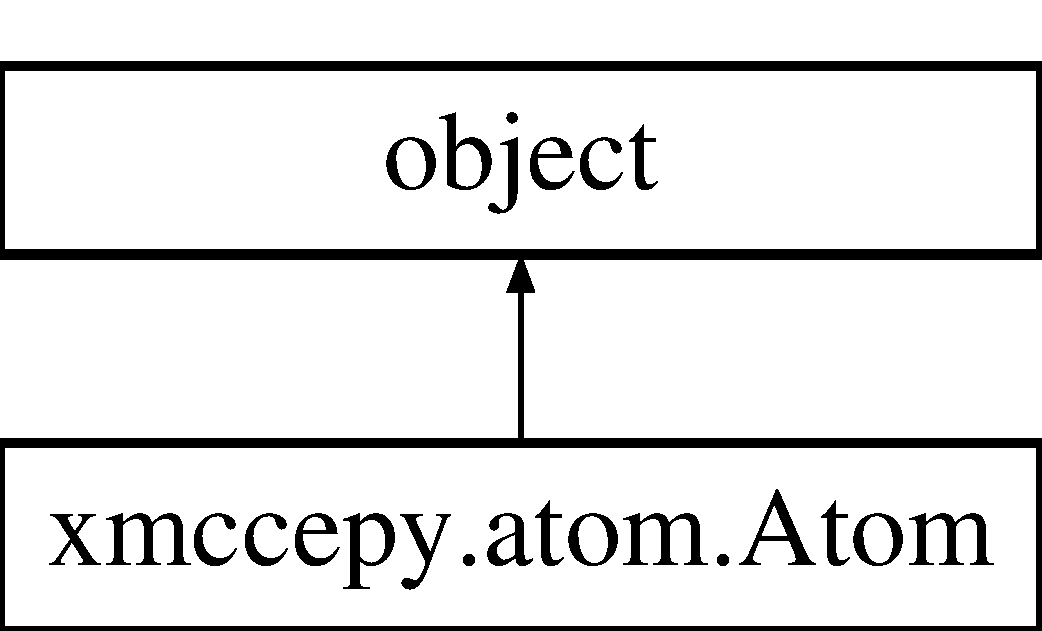
\includegraphics[height=2.000000cm]{classxmccepy_1_1atom_1_1_atom}
\end{center}
\end{figure}
\subsection*{Public Member Functions}
\begin{DoxyCompactItemize}
\item 
def \hyperlink{classxmccepy_1_1atom_1_1_atom_a1964c39c0d09b6867c35ad3ad95c4f06}{\-\_\-\-\_\-init\-\_\-\-\_\-}
\begin{DoxyCompactList}\small\item\em Constructor. \end{DoxyCompactList}\item 
def \hyperlink{classxmccepy_1_1atom_1_1_atom_ae2e395a615e79abe1dd1c5f0ce3d0c90}{set\-Corr}
\begin{DoxyCompactList}\small\item\em Set the coordinate of the atom. \end{DoxyCompactList}\item 
def \hyperlink{classxmccepy_1_1atom_1_1_atom_af43673725714087009243eadbc7f95a7}{read\-Step1\-Line}
\begin{DoxyCompactList}\small\item\em Read a line in step1\-\_\-out.\-pdb. \end{DoxyCompactList}\item 
def \hyperlink{classxmccepy_1_1atom_1_1_atom_a5f3516b8720c26ba0712f7b6066c1cf4}{write\-Step1\-Line}
\begin{DoxyCompactList}\small\item\em Write atom like a line in step1\-\_\-out.\-pdb. \end{DoxyCompactList}\item 
def \hyperlink{classxmccepy_1_1atom_1_1_atom_a36929050f7e6a8728a3525a3eb58b044}{read\-Pdb\-Line}
\begin{DoxyCompactList}\small\item\em Read a line in a standard pdb file. \end{DoxyCompactList}\item 
def \hyperlink{classxmccepy_1_1atom_1_1_atom_a19708571103d9d925eaa23d07a7963d8}{write\-Pdb\-Line}
\begin{DoxyCompactList}\small\item\em Write atom like a line in standard pdb file. \end{DoxyCompactList}\end{DoxyCompactItemize}
\subsection*{Public Attributes}
\begin{DoxyCompactItemize}
\item 
\hyperlink{classxmccepy_1_1atom_1_1_atom_ad394fcd2eca6340dcd5d832a1bd0ec8a}{group\-Id}
\begin{DoxyCompactList}\small\item\em A\-T\-O\-M or H\-E\-T\-A\-T\-M. \end{DoxyCompactList}\item 
\hyperlink{classxmccepy_1_1atom_1_1_atom_a4c4c032cdb4a5f7e5df6f78c10d11629}{atom\-Seq}
\item 
\hyperlink{classxmccepy_1_1atom_1_1_atom_a410419d5a7bcf8e5bb504c393c03849f}{atom\-Name}
\begin{DoxyCompactList}\small\item\em Four letter standard name as in tpl file. \end{DoxyCompactList}\item 
\hyperlink{classxmccepy_1_1atom_1_1_atom_a7fe1185c33a55254824b54ef1218de51}{res\-Name}
\item 
\hyperlink{classxmccepy_1_1atom_1_1_atom_acd780de97bd09f7eba1a6f1067badbf0}{chain\-Id}
\item 
\hyperlink{classxmccepy_1_1atom_1_1_atom_a539eb962040217d58384463edbc73718}{res\-Seq}
\item 
\hyperlink{classxmccepy_1_1atom_1_1_atom_af11e5763e17aa49dd9ceeb73496a3eb5}{conf\-Seq}
\item 
\hyperlink{classxmccepy_1_1atom_1_1_atom_af3e01f96338f93fbcc67765c4d668066}{corr}
\item 
\hyperlink{classxmccepy_1_1atom_1_1_atom_af0235fff236afb4e97011731adb22f55}{radius}
\item 
\hyperlink{classxmccepy_1_1atom_1_1_atom_a75da5d014806b57f4bc26095aa5f8c80}{charge}
\item 
\hyperlink{classxmccepy_1_1atom_1_1_atom_a40df064eecfddbd9a84044c42742ca53}{history}
\item 
\hyperlink{classxmccepy_1_1atom_1_1_atom_a0ae57fea9163a481424524a4a57fb1de}{pdb\-Rest}
\begin{DoxyCompactList}\small\item\em The trailing part of a pdb line which is not parsed. \end{DoxyCompactList}\end{DoxyCompactItemize}


\subsection{Detailed Description}
\hyperlink{classxmccepy_1_1atom_1_1_atom}{Atom} class. 

\subsection{Constructor \& Destructor Documentation}
\hypertarget{classxmccepy_1_1atom_1_1_atom_a1964c39c0d09b6867c35ad3ad95c4f06}{\index{xmccepy\-::atom\-::\-Atom@{xmccepy\-::atom\-::\-Atom}!\-\_\-\-\_\-init\-\_\-\-\_\-@{\-\_\-\-\_\-init\-\_\-\-\_\-}}
\index{\-\_\-\-\_\-init\-\_\-\-\_\-@{\-\_\-\-\_\-init\-\_\-\-\_\-}!xmccepy::atom::Atom@{xmccepy\-::atom\-::\-Atom}}
\subsubsection[{\-\_\-\-\_\-init\-\_\-\-\_\-}]{\setlength{\rightskip}{0pt plus 5cm}def xmccepy.\-atom.\-Atom.\-\_\-\-\_\-init\-\_\-\-\_\- (
\begin{DoxyParamCaption}
\item[{}]{self}
\end{DoxyParamCaption}
)}}\label{classxmccepy_1_1atom_1_1_atom_a1964c39c0d09b6867c35ad3ad95c4f06}


Constructor. 



\subsection{Member Function Documentation}
\hypertarget{classxmccepy_1_1atom_1_1_atom_a36929050f7e6a8728a3525a3eb58b044}{\index{xmccepy\-::atom\-::\-Atom@{xmccepy\-::atom\-::\-Atom}!read\-Pdb\-Line@{read\-Pdb\-Line}}
\index{read\-Pdb\-Line@{read\-Pdb\-Line}!xmccepy::atom::Atom@{xmccepy\-::atom\-::\-Atom}}
\subsubsection[{read\-Pdb\-Line}]{\setlength{\rightskip}{0pt plus 5cm}def xmccepy.\-atom.\-Atom.\-read\-Pdb\-Line (
\begin{DoxyParamCaption}
\item[{}]{self, }
\item[{}]{pline}
\end{DoxyParamCaption}
)}}\label{classxmccepy_1_1atom_1_1_atom_a36929050f7e6a8728a3525a3eb58b044}


Read a line in a standard pdb file. 


\begin{DoxyParams}{Parameters}
{\em pline} & A line in pdb file. \\
\hline
\end{DoxyParams}
\hypertarget{classxmccepy_1_1atom_1_1_atom_af43673725714087009243eadbc7f95a7}{\index{xmccepy\-::atom\-::\-Atom@{xmccepy\-::atom\-::\-Atom}!read\-Step1\-Line@{read\-Step1\-Line}}
\index{read\-Step1\-Line@{read\-Step1\-Line}!xmccepy::atom::Atom@{xmccepy\-::atom\-::\-Atom}}
\subsubsection[{read\-Step1\-Line}]{\setlength{\rightskip}{0pt plus 5cm}def xmccepy.\-atom.\-Atom.\-read\-Step1\-Line (
\begin{DoxyParamCaption}
\item[{}]{self, }
\item[{}]{sline}
\end{DoxyParamCaption}
)}}\label{classxmccepy_1_1atom_1_1_atom_af43673725714087009243eadbc7f95a7}


Read a line in step1\-\_\-out.\-pdb. 

A line in step1\-\_\-out.\-pdb represents an atom with extra info about the conformer. 
\begin{DoxyParams}{Parameters}
{\em sline} & A line from step1\-\_\-out.\-pdb. \\
\hline
\end{DoxyParams}
\hypertarget{classxmccepy_1_1atom_1_1_atom_ae2e395a615e79abe1dd1c5f0ce3d0c90}{\index{xmccepy\-::atom\-::\-Atom@{xmccepy\-::atom\-::\-Atom}!set\-Corr@{set\-Corr}}
\index{set\-Corr@{set\-Corr}!xmccepy::atom::Atom@{xmccepy\-::atom\-::\-Atom}}
\subsubsection[{set\-Corr}]{\setlength{\rightskip}{0pt plus 5cm}def xmccepy.\-atom.\-Atom.\-set\-Corr (
\begin{DoxyParamCaption}
\item[{}]{self, }
\item[{}]{x = {\ttfamily 0.0}, }
\item[{}]{y = {\ttfamily 0.0}, }
\item[{}]{z = {\ttfamily 0.0}}
\end{DoxyParamCaption}
)}}\label{classxmccepy_1_1atom_1_1_atom_ae2e395a615e79abe1dd1c5f0ce3d0c90}


Set the coordinate of the atom. 

\hypertarget{classxmccepy_1_1atom_1_1_atom_a19708571103d9d925eaa23d07a7963d8}{\index{xmccepy\-::atom\-::\-Atom@{xmccepy\-::atom\-::\-Atom}!write\-Pdb\-Line@{write\-Pdb\-Line}}
\index{write\-Pdb\-Line@{write\-Pdb\-Line}!xmccepy::atom::Atom@{xmccepy\-::atom\-::\-Atom}}
\subsubsection[{write\-Pdb\-Line}]{\setlength{\rightskip}{0pt plus 5cm}def xmccepy.\-atom.\-Atom.\-write\-Pdb\-Line (
\begin{DoxyParamCaption}
\item[{}]{self}
\end{DoxyParamCaption}
)}}\label{classxmccepy_1_1atom_1_1_atom_a19708571103d9d925eaa23d07a7963d8}


Write atom like a line in standard pdb file. 

\begin{DoxyReturn}{Returns}
A line of atom for pdb file. 
\end{DoxyReturn}
\hypertarget{classxmccepy_1_1atom_1_1_atom_a5f3516b8720c26ba0712f7b6066c1cf4}{\index{xmccepy\-::atom\-::\-Atom@{xmccepy\-::atom\-::\-Atom}!write\-Step1\-Line@{write\-Step1\-Line}}
\index{write\-Step1\-Line@{write\-Step1\-Line}!xmccepy::atom::Atom@{xmccepy\-::atom\-::\-Atom}}
\subsubsection[{write\-Step1\-Line}]{\setlength{\rightskip}{0pt plus 5cm}def xmccepy.\-atom.\-Atom.\-write\-Step1\-Line (
\begin{DoxyParamCaption}
\item[{}]{self}
\end{DoxyParamCaption}
)}}\label{classxmccepy_1_1atom_1_1_atom_a5f3516b8720c26ba0712f7b6066c1cf4}


Write atom like a line in step1\-\_\-out.\-pdb. 

\begin{DoxyReturn}{Returns}
A line of atom for step1\-\_\-out.\-pdb. 
\end{DoxyReturn}


\subsection{Member Data Documentation}
\hypertarget{classxmccepy_1_1atom_1_1_atom_a410419d5a7bcf8e5bb504c393c03849f}{\index{xmccepy\-::atom\-::\-Atom@{xmccepy\-::atom\-::\-Atom}!atom\-Name@{atom\-Name}}
\index{atom\-Name@{atom\-Name}!xmccepy::atom::Atom@{xmccepy\-::atom\-::\-Atom}}
\subsubsection[{atom\-Name}]{\setlength{\rightskip}{0pt plus 5cm}xmccepy.\-atom.\-Atom.\-atom\-Name}}\label{classxmccepy_1_1atom_1_1_atom_a410419d5a7bcf8e5bb504c393c03849f}


Four letter standard name as in tpl file. 

\hypertarget{classxmccepy_1_1atom_1_1_atom_a4c4c032cdb4a5f7e5df6f78c10d11629}{\index{xmccepy\-::atom\-::\-Atom@{xmccepy\-::atom\-::\-Atom}!atom\-Seq@{atom\-Seq}}
\index{atom\-Seq@{atom\-Seq}!xmccepy::atom::Atom@{xmccepy\-::atom\-::\-Atom}}
\subsubsection[{atom\-Seq}]{\setlength{\rightskip}{0pt plus 5cm}xmccepy.\-atom.\-Atom.\-atom\-Seq}}\label{classxmccepy_1_1atom_1_1_atom_a4c4c032cdb4a5f7e5df6f78c10d11629}
\hypertarget{classxmccepy_1_1atom_1_1_atom_acd780de97bd09f7eba1a6f1067badbf0}{\index{xmccepy\-::atom\-::\-Atom@{xmccepy\-::atom\-::\-Atom}!chain\-Id@{chain\-Id}}
\index{chain\-Id@{chain\-Id}!xmccepy::atom::Atom@{xmccepy\-::atom\-::\-Atom}}
\subsubsection[{chain\-Id}]{\setlength{\rightskip}{0pt plus 5cm}xmccepy.\-atom.\-Atom.\-chain\-Id}}\label{classxmccepy_1_1atom_1_1_atom_acd780de97bd09f7eba1a6f1067badbf0}
\hypertarget{classxmccepy_1_1atom_1_1_atom_a75da5d014806b57f4bc26095aa5f8c80}{\index{xmccepy\-::atom\-::\-Atom@{xmccepy\-::atom\-::\-Atom}!charge@{charge}}
\index{charge@{charge}!xmccepy::atom::Atom@{xmccepy\-::atom\-::\-Atom}}
\subsubsection[{charge}]{\setlength{\rightskip}{0pt plus 5cm}xmccepy.\-atom.\-Atom.\-charge}}\label{classxmccepy_1_1atom_1_1_atom_a75da5d014806b57f4bc26095aa5f8c80}
\hypertarget{classxmccepy_1_1atom_1_1_atom_af11e5763e17aa49dd9ceeb73496a3eb5}{\index{xmccepy\-::atom\-::\-Atom@{xmccepy\-::atom\-::\-Atom}!conf\-Seq@{conf\-Seq}}
\index{conf\-Seq@{conf\-Seq}!xmccepy::atom::Atom@{xmccepy\-::atom\-::\-Atom}}
\subsubsection[{conf\-Seq}]{\setlength{\rightskip}{0pt plus 5cm}xmccepy.\-atom.\-Atom.\-conf\-Seq}}\label{classxmccepy_1_1atom_1_1_atom_af11e5763e17aa49dd9ceeb73496a3eb5}
\hypertarget{classxmccepy_1_1atom_1_1_atom_af3e01f96338f93fbcc67765c4d668066}{\index{xmccepy\-::atom\-::\-Atom@{xmccepy\-::atom\-::\-Atom}!corr@{corr}}
\index{corr@{corr}!xmccepy::atom::Atom@{xmccepy\-::atom\-::\-Atom}}
\subsubsection[{corr}]{\setlength{\rightskip}{0pt plus 5cm}xmccepy.\-atom.\-Atom.\-corr}}\label{classxmccepy_1_1atom_1_1_atom_af3e01f96338f93fbcc67765c4d668066}
\hypertarget{classxmccepy_1_1atom_1_1_atom_ad394fcd2eca6340dcd5d832a1bd0ec8a}{\index{xmccepy\-::atom\-::\-Atom@{xmccepy\-::atom\-::\-Atom}!group\-Id@{group\-Id}}
\index{group\-Id@{group\-Id}!xmccepy::atom::Atom@{xmccepy\-::atom\-::\-Atom}}
\subsubsection[{group\-Id}]{\setlength{\rightskip}{0pt plus 5cm}xmccepy.\-atom.\-Atom.\-group\-Id}}\label{classxmccepy_1_1atom_1_1_atom_ad394fcd2eca6340dcd5d832a1bd0ec8a}


A\-T\-O\-M or H\-E\-T\-A\-T\-M. 

\hypertarget{classxmccepy_1_1atom_1_1_atom_a40df064eecfddbd9a84044c42742ca53}{\index{xmccepy\-::atom\-::\-Atom@{xmccepy\-::atom\-::\-Atom}!history@{history}}
\index{history@{history}!xmccepy::atom::Atom@{xmccepy\-::atom\-::\-Atom}}
\subsubsection[{history}]{\setlength{\rightskip}{0pt plus 5cm}xmccepy.\-atom.\-Atom.\-history}}\label{classxmccepy_1_1atom_1_1_atom_a40df064eecfddbd9a84044c42742ca53}
\hypertarget{classxmccepy_1_1atom_1_1_atom_a0ae57fea9163a481424524a4a57fb1de}{\index{xmccepy\-::atom\-::\-Atom@{xmccepy\-::atom\-::\-Atom}!pdb\-Rest@{pdb\-Rest}}
\index{pdb\-Rest@{pdb\-Rest}!xmccepy::atom::Atom@{xmccepy\-::atom\-::\-Atom}}
\subsubsection[{pdb\-Rest}]{\setlength{\rightskip}{0pt plus 5cm}xmccepy.\-atom.\-Atom.\-pdb\-Rest}}\label{classxmccepy_1_1atom_1_1_atom_a0ae57fea9163a481424524a4a57fb1de}


The trailing part of a pdb line which is not parsed. 

\hypertarget{classxmccepy_1_1atom_1_1_atom_af0235fff236afb4e97011731adb22f55}{\index{xmccepy\-::atom\-::\-Atom@{xmccepy\-::atom\-::\-Atom}!radius@{radius}}
\index{radius@{radius}!xmccepy::atom::Atom@{xmccepy\-::atom\-::\-Atom}}
\subsubsection[{radius}]{\setlength{\rightskip}{0pt plus 5cm}xmccepy.\-atom.\-Atom.\-radius}}\label{classxmccepy_1_1atom_1_1_atom_af0235fff236afb4e97011731adb22f55}
\hypertarget{classxmccepy_1_1atom_1_1_atom_a7fe1185c33a55254824b54ef1218de51}{\index{xmccepy\-::atom\-::\-Atom@{xmccepy\-::atom\-::\-Atom}!res\-Name@{res\-Name}}
\index{res\-Name@{res\-Name}!xmccepy::atom::Atom@{xmccepy\-::atom\-::\-Atom}}
\subsubsection[{res\-Name}]{\setlength{\rightskip}{0pt plus 5cm}xmccepy.\-atom.\-Atom.\-res\-Name}}\label{classxmccepy_1_1atom_1_1_atom_a7fe1185c33a55254824b54ef1218de51}
\hypertarget{classxmccepy_1_1atom_1_1_atom_a539eb962040217d58384463edbc73718}{\index{xmccepy\-::atom\-::\-Atom@{xmccepy\-::atom\-::\-Atom}!res\-Seq@{res\-Seq}}
\index{res\-Seq@{res\-Seq}!xmccepy::atom::Atom@{xmccepy\-::atom\-::\-Atom}}
\subsubsection[{res\-Seq}]{\setlength{\rightskip}{0pt plus 5cm}xmccepy.\-atom.\-Atom.\-res\-Seq}}\label{classxmccepy_1_1atom_1_1_atom_a539eb962040217d58384463edbc73718}


The documentation for this class was generated from the following file\-:\begin{DoxyCompactItemize}
\item 
src/xmccepy/\hyperlink{atom_8py}{atom.\-py}\end{DoxyCompactItemize}

\hypertarget{classxmccepy_1_1mp_1_1_a_t_o_m}{\section{xmccepy.\-mp.\-A\-T\-O\-M Class Reference}
\label{classxmccepy_1_1mp_1_1_a_t_o_m}\index{xmccepy.\-mp.\-A\-T\-O\-M@{xmccepy.\-mp.\-A\-T\-O\-M}}
}
\subsection*{Public Member Functions}
\begin{DoxyCompactItemize}
\item 
def \hyperlink{classxmccepy_1_1mp_1_1_a_t_o_m_aa6e2fb4b7c8efc44b26b2b21964db907}{\-\_\-\-\_\-init\-\_\-\-\_\-}
\item 
def \hyperlink{classxmccepy_1_1mp_1_1_a_t_o_m_a136255ca36ba6682255e0c3c16b49c39}{load\-Step\-Line}
\end{DoxyCompactItemize}
\subsection*{Public Attributes}
\begin{DoxyCompactItemize}
\item 
\hyperlink{classxmccepy_1_1mp_1_1_a_t_o_m_a2cef52139b5235586607f4ba6fe44ee9}{serial}
\item 
\hyperlink{classxmccepy_1_1mp_1_1_a_t_o_m_a54ade2663ba22d42473d82bbb0731451}{name}
\item 
\hyperlink{classxmccepy_1_1mp_1_1_a_t_o_m_afbc19b6c21ca49dbe761479669a24c66}{alt\-Loc}
\item 
\hyperlink{classxmccepy_1_1mp_1_1_a_t_o_m_a8f4bed4463123a6d83abd93f69438ebe}{res\-Name}
\item 
\hyperlink{classxmccepy_1_1mp_1_1_a_t_o_m_a253ac66ab99349121fda0a6183f10a12}{chain\-I\-D}
\item 
\hyperlink{classxmccepy_1_1mp_1_1_a_t_o_m_ac91c801a2d8279659c74c69e820215a9}{res\-Seq}
\item 
\hyperlink{classxmccepy_1_1mp_1_1_a_t_o_m_a7ace60261d88bcbcd23f5e14a86b77e6}{i\-Code}
\item 
\hyperlink{classxmccepy_1_1mp_1_1_a_t_o_m_aebf9f0b985ccd236b1cd2dbf1161941e}{xyz}
\item 
\hyperlink{classxmccepy_1_1mp_1_1_a_t_o_m_ae56b3a55f15835108b393b32f6ac1878}{rad}
\item 
\hyperlink{classxmccepy_1_1mp_1_1_a_t_o_m_a0e3bac6ace5f4cc33db8eb20120764d4}{crg}
\item 
\hyperlink{classxmccepy_1_1mp_1_1_a_t_o_m_aa3702294f6091d253474476bfcd35f34}{history}
\end{DoxyCompactItemize}


\subsection{Constructor \& Destructor Documentation}
\hypertarget{classxmccepy_1_1mp_1_1_a_t_o_m_aa6e2fb4b7c8efc44b26b2b21964db907}{\index{xmccepy\-::mp\-::\-A\-T\-O\-M@{xmccepy\-::mp\-::\-A\-T\-O\-M}!\-\_\-\-\_\-init\-\_\-\-\_\-@{\-\_\-\-\_\-init\-\_\-\-\_\-}}
\index{\-\_\-\-\_\-init\-\_\-\-\_\-@{\-\_\-\-\_\-init\-\_\-\-\_\-}!xmccepy::mp::ATOM@{xmccepy\-::mp\-::\-A\-T\-O\-M}}
\subsubsection[{\-\_\-\-\_\-init\-\_\-\-\_\-}]{\setlength{\rightskip}{0pt plus 5cm}def xmccepy.\-mp.\-A\-T\-O\-M.\-\_\-\-\_\-init\-\_\-\-\_\- (
\begin{DoxyParamCaption}
\item[{}]{self}
\end{DoxyParamCaption}
)}}\label{classxmccepy_1_1mp_1_1_a_t_o_m_aa6e2fb4b7c8efc44b26b2b21964db907}


\subsection{Member Function Documentation}
\hypertarget{classxmccepy_1_1mp_1_1_a_t_o_m_a136255ca36ba6682255e0c3c16b49c39}{\index{xmccepy\-::mp\-::\-A\-T\-O\-M@{xmccepy\-::mp\-::\-A\-T\-O\-M}!load\-Step\-Line@{load\-Step\-Line}}
\index{load\-Step\-Line@{load\-Step\-Line}!xmccepy::mp::ATOM@{xmccepy\-::mp\-::\-A\-T\-O\-M}}
\subsubsection[{load\-Step\-Line}]{\setlength{\rightskip}{0pt plus 5cm}def xmccepy.\-mp.\-A\-T\-O\-M.\-load\-Step\-Line (
\begin{DoxyParamCaption}
\item[{}]{self, }
\item[{}]{line}
\end{DoxyParamCaption}
)}}\label{classxmccepy_1_1mp_1_1_a_t_o_m_a136255ca36ba6682255e0c3c16b49c39}


\subsection{Member Data Documentation}
\hypertarget{classxmccepy_1_1mp_1_1_a_t_o_m_afbc19b6c21ca49dbe761479669a24c66}{\index{xmccepy\-::mp\-::\-A\-T\-O\-M@{xmccepy\-::mp\-::\-A\-T\-O\-M}!alt\-Loc@{alt\-Loc}}
\index{alt\-Loc@{alt\-Loc}!xmccepy::mp::ATOM@{xmccepy\-::mp\-::\-A\-T\-O\-M}}
\subsubsection[{alt\-Loc}]{\setlength{\rightskip}{0pt plus 5cm}xmccepy.\-mp.\-A\-T\-O\-M.\-alt\-Loc}}\label{classxmccepy_1_1mp_1_1_a_t_o_m_afbc19b6c21ca49dbe761479669a24c66}
\hypertarget{classxmccepy_1_1mp_1_1_a_t_o_m_a253ac66ab99349121fda0a6183f10a12}{\index{xmccepy\-::mp\-::\-A\-T\-O\-M@{xmccepy\-::mp\-::\-A\-T\-O\-M}!chain\-I\-D@{chain\-I\-D}}
\index{chain\-I\-D@{chain\-I\-D}!xmccepy::mp::ATOM@{xmccepy\-::mp\-::\-A\-T\-O\-M}}
\subsubsection[{chain\-I\-D}]{\setlength{\rightskip}{0pt plus 5cm}xmccepy.\-mp.\-A\-T\-O\-M.\-chain\-I\-D}}\label{classxmccepy_1_1mp_1_1_a_t_o_m_a253ac66ab99349121fda0a6183f10a12}
\hypertarget{classxmccepy_1_1mp_1_1_a_t_o_m_a0e3bac6ace5f4cc33db8eb20120764d4}{\index{xmccepy\-::mp\-::\-A\-T\-O\-M@{xmccepy\-::mp\-::\-A\-T\-O\-M}!crg@{crg}}
\index{crg@{crg}!xmccepy::mp::ATOM@{xmccepy\-::mp\-::\-A\-T\-O\-M}}
\subsubsection[{crg}]{\setlength{\rightskip}{0pt plus 5cm}xmccepy.\-mp.\-A\-T\-O\-M.\-crg}}\label{classxmccepy_1_1mp_1_1_a_t_o_m_a0e3bac6ace5f4cc33db8eb20120764d4}
\hypertarget{classxmccepy_1_1mp_1_1_a_t_o_m_aa3702294f6091d253474476bfcd35f34}{\index{xmccepy\-::mp\-::\-A\-T\-O\-M@{xmccepy\-::mp\-::\-A\-T\-O\-M}!history@{history}}
\index{history@{history}!xmccepy::mp::ATOM@{xmccepy\-::mp\-::\-A\-T\-O\-M}}
\subsubsection[{history}]{\setlength{\rightskip}{0pt plus 5cm}xmccepy.\-mp.\-A\-T\-O\-M.\-history}}\label{classxmccepy_1_1mp_1_1_a_t_o_m_aa3702294f6091d253474476bfcd35f34}
\hypertarget{classxmccepy_1_1mp_1_1_a_t_o_m_a7ace60261d88bcbcd23f5e14a86b77e6}{\index{xmccepy\-::mp\-::\-A\-T\-O\-M@{xmccepy\-::mp\-::\-A\-T\-O\-M}!i\-Code@{i\-Code}}
\index{i\-Code@{i\-Code}!xmccepy::mp::ATOM@{xmccepy\-::mp\-::\-A\-T\-O\-M}}
\subsubsection[{i\-Code}]{\setlength{\rightskip}{0pt plus 5cm}xmccepy.\-mp.\-A\-T\-O\-M.\-i\-Code}}\label{classxmccepy_1_1mp_1_1_a_t_o_m_a7ace60261d88bcbcd23f5e14a86b77e6}
\hypertarget{classxmccepy_1_1mp_1_1_a_t_o_m_a54ade2663ba22d42473d82bbb0731451}{\index{xmccepy\-::mp\-::\-A\-T\-O\-M@{xmccepy\-::mp\-::\-A\-T\-O\-M}!name@{name}}
\index{name@{name}!xmccepy::mp::ATOM@{xmccepy\-::mp\-::\-A\-T\-O\-M}}
\subsubsection[{name}]{\setlength{\rightskip}{0pt plus 5cm}xmccepy.\-mp.\-A\-T\-O\-M.\-name}}\label{classxmccepy_1_1mp_1_1_a_t_o_m_a54ade2663ba22d42473d82bbb0731451}
\hypertarget{classxmccepy_1_1mp_1_1_a_t_o_m_ae56b3a55f15835108b393b32f6ac1878}{\index{xmccepy\-::mp\-::\-A\-T\-O\-M@{xmccepy\-::mp\-::\-A\-T\-O\-M}!rad@{rad}}
\index{rad@{rad}!xmccepy::mp::ATOM@{xmccepy\-::mp\-::\-A\-T\-O\-M}}
\subsubsection[{rad}]{\setlength{\rightskip}{0pt plus 5cm}xmccepy.\-mp.\-A\-T\-O\-M.\-rad}}\label{classxmccepy_1_1mp_1_1_a_t_o_m_ae56b3a55f15835108b393b32f6ac1878}
\hypertarget{classxmccepy_1_1mp_1_1_a_t_o_m_a8f4bed4463123a6d83abd93f69438ebe}{\index{xmccepy\-::mp\-::\-A\-T\-O\-M@{xmccepy\-::mp\-::\-A\-T\-O\-M}!res\-Name@{res\-Name}}
\index{res\-Name@{res\-Name}!xmccepy::mp::ATOM@{xmccepy\-::mp\-::\-A\-T\-O\-M}}
\subsubsection[{res\-Name}]{\setlength{\rightskip}{0pt plus 5cm}xmccepy.\-mp.\-A\-T\-O\-M.\-res\-Name}}\label{classxmccepy_1_1mp_1_1_a_t_o_m_a8f4bed4463123a6d83abd93f69438ebe}
\hypertarget{classxmccepy_1_1mp_1_1_a_t_o_m_ac91c801a2d8279659c74c69e820215a9}{\index{xmccepy\-::mp\-::\-A\-T\-O\-M@{xmccepy\-::mp\-::\-A\-T\-O\-M}!res\-Seq@{res\-Seq}}
\index{res\-Seq@{res\-Seq}!xmccepy::mp::ATOM@{xmccepy\-::mp\-::\-A\-T\-O\-M}}
\subsubsection[{res\-Seq}]{\setlength{\rightskip}{0pt plus 5cm}xmccepy.\-mp.\-A\-T\-O\-M.\-res\-Seq}}\label{classxmccepy_1_1mp_1_1_a_t_o_m_ac91c801a2d8279659c74c69e820215a9}
\hypertarget{classxmccepy_1_1mp_1_1_a_t_o_m_a2cef52139b5235586607f4ba6fe44ee9}{\index{xmccepy\-::mp\-::\-A\-T\-O\-M@{xmccepy\-::mp\-::\-A\-T\-O\-M}!serial@{serial}}
\index{serial@{serial}!xmccepy::mp::ATOM@{xmccepy\-::mp\-::\-A\-T\-O\-M}}
\subsubsection[{serial}]{\setlength{\rightskip}{0pt plus 5cm}xmccepy.\-mp.\-A\-T\-O\-M.\-serial}}\label{classxmccepy_1_1mp_1_1_a_t_o_m_a2cef52139b5235586607f4ba6fe44ee9}
\hypertarget{classxmccepy_1_1mp_1_1_a_t_o_m_aebf9f0b985ccd236b1cd2dbf1161941e}{\index{xmccepy\-::mp\-::\-A\-T\-O\-M@{xmccepy\-::mp\-::\-A\-T\-O\-M}!xyz@{xyz}}
\index{xyz@{xyz}!xmccepy::mp::ATOM@{xmccepy\-::mp\-::\-A\-T\-O\-M}}
\subsubsection[{xyz}]{\setlength{\rightskip}{0pt plus 5cm}xmccepy.\-mp.\-A\-T\-O\-M.\-xyz}}\label{classxmccepy_1_1mp_1_1_a_t_o_m_aebf9f0b985ccd236b1cd2dbf1161941e}


The documentation for this class was generated from the following file\-:\begin{DoxyCompactItemize}
\item 
src/xmccepy/\hyperlink{mp_8py}{mp.\-py}\end{DoxyCompactItemize}

\hypertarget{classstep1__to__pdb_1_1_c_l_i_error}{\section{step1\-\_\-to\-\_\-pdb.\-C\-L\-I\-Error Class Reference}
\label{classstep1__to__pdb_1_1_c_l_i_error}\index{step1\-\_\-to\-\_\-pdb.\-C\-L\-I\-Error@{step1\-\_\-to\-\_\-pdb.\-C\-L\-I\-Error}}
}


Generic exception to raise and log different fatal errors.  


Inheritance diagram for step1\-\_\-to\-\_\-pdb.\-C\-L\-I\-Error\-:\begin{figure}[H]
\begin{center}
\leavevmode
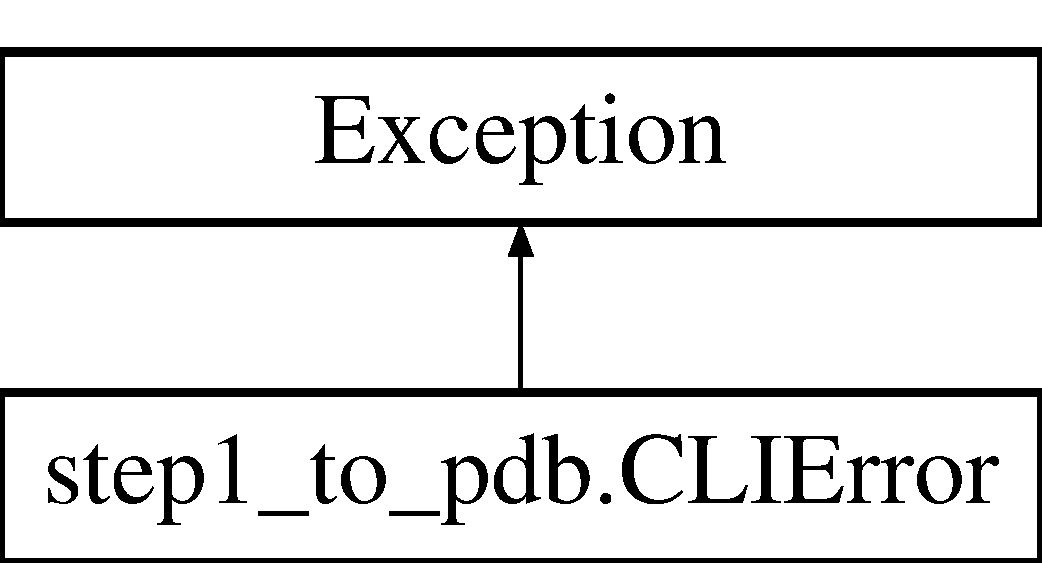
\includegraphics[height=2.000000cm]{classstep1__to__pdb_1_1_c_l_i_error}
\end{center}
\end{figure}
\subsection*{Public Member Functions}
\begin{DoxyCompactItemize}
\item 
def \hyperlink{classstep1__to__pdb_1_1_c_l_i_error_af7ef908bc07f68e5f79a620dde83dba0}{\-\_\-\-\_\-init\-\_\-\-\_\-}
\item 
def \hyperlink{classstep1__to__pdb_1_1_c_l_i_error_a75c25a11ea5c4ab13bc7970fc85e8487}{\-\_\-\-\_\-str\-\_\-\-\_\-}
\item 
def \hyperlink{classstep1__to__pdb_1_1_c_l_i_error_a5227949d447b7d28c3fec0983891c004}{\-\_\-\-\_\-unicode\-\_\-\-\_\-}
\end{DoxyCompactItemize}
\subsection*{Public Attributes}
\begin{DoxyCompactItemize}
\item 
\hyperlink{classstep1__to__pdb_1_1_c_l_i_error_adc73a367f4c49d59a08eb66d2d95dfc5}{msg}
\end{DoxyCompactItemize}


\subsection{Detailed Description}
Generic exception to raise and log different fatal errors. 



\subsection{Constructor \& Destructor Documentation}
\hypertarget{classstep1__to__pdb_1_1_c_l_i_error_af7ef908bc07f68e5f79a620dde83dba0}{\index{step1\-\_\-to\-\_\-pdb\-::\-C\-L\-I\-Error@{step1\-\_\-to\-\_\-pdb\-::\-C\-L\-I\-Error}!\-\_\-\-\_\-init\-\_\-\-\_\-@{\-\_\-\-\_\-init\-\_\-\-\_\-}}
\index{\-\_\-\-\_\-init\-\_\-\-\_\-@{\-\_\-\-\_\-init\-\_\-\-\_\-}!step1_to_pdb::CLIError@{step1\-\_\-to\-\_\-pdb\-::\-C\-L\-I\-Error}}
\subsubsection[{\-\_\-\-\_\-init\-\_\-\-\_\-}]{\setlength{\rightskip}{0pt plus 5cm}def step1\-\_\-to\-\_\-pdb.\-C\-L\-I\-Error.\-\_\-\-\_\-init\-\_\-\-\_\- (
\begin{DoxyParamCaption}
\item[{}]{self, }
\item[{}]{msg}
\end{DoxyParamCaption}
)}}\label{classstep1__to__pdb_1_1_c_l_i_error_af7ef908bc07f68e5f79a620dde83dba0}


\subsection{Member Function Documentation}
\hypertarget{classstep1__to__pdb_1_1_c_l_i_error_a75c25a11ea5c4ab13bc7970fc85e8487}{\index{step1\-\_\-to\-\_\-pdb\-::\-C\-L\-I\-Error@{step1\-\_\-to\-\_\-pdb\-::\-C\-L\-I\-Error}!\-\_\-\-\_\-str\-\_\-\-\_\-@{\-\_\-\-\_\-str\-\_\-\-\_\-}}
\index{\-\_\-\-\_\-str\-\_\-\-\_\-@{\-\_\-\-\_\-str\-\_\-\-\_\-}!step1_to_pdb::CLIError@{step1\-\_\-to\-\_\-pdb\-::\-C\-L\-I\-Error}}
\subsubsection[{\-\_\-\-\_\-str\-\_\-\-\_\-}]{\setlength{\rightskip}{0pt plus 5cm}def step1\-\_\-to\-\_\-pdb.\-C\-L\-I\-Error.\-\_\-\-\_\-str\-\_\-\-\_\- (
\begin{DoxyParamCaption}
\item[{}]{self}
\end{DoxyParamCaption}
)}}\label{classstep1__to__pdb_1_1_c_l_i_error_a75c25a11ea5c4ab13bc7970fc85e8487}
\hypertarget{classstep1__to__pdb_1_1_c_l_i_error_a5227949d447b7d28c3fec0983891c004}{\index{step1\-\_\-to\-\_\-pdb\-::\-C\-L\-I\-Error@{step1\-\_\-to\-\_\-pdb\-::\-C\-L\-I\-Error}!\-\_\-\-\_\-unicode\-\_\-\-\_\-@{\-\_\-\-\_\-unicode\-\_\-\-\_\-}}
\index{\-\_\-\-\_\-unicode\-\_\-\-\_\-@{\-\_\-\-\_\-unicode\-\_\-\-\_\-}!step1_to_pdb::CLIError@{step1\-\_\-to\-\_\-pdb\-::\-C\-L\-I\-Error}}
\subsubsection[{\-\_\-\-\_\-unicode\-\_\-\-\_\-}]{\setlength{\rightskip}{0pt plus 5cm}def step1\-\_\-to\-\_\-pdb.\-C\-L\-I\-Error.\-\_\-\-\_\-unicode\-\_\-\-\_\- (
\begin{DoxyParamCaption}
\item[{}]{self}
\end{DoxyParamCaption}
)}}\label{classstep1__to__pdb_1_1_c_l_i_error_a5227949d447b7d28c3fec0983891c004}


\subsection{Member Data Documentation}
\hypertarget{classstep1__to__pdb_1_1_c_l_i_error_adc73a367f4c49d59a08eb66d2d95dfc5}{\index{step1\-\_\-to\-\_\-pdb\-::\-C\-L\-I\-Error@{step1\-\_\-to\-\_\-pdb\-::\-C\-L\-I\-Error}!msg@{msg}}
\index{msg@{msg}!step1_to_pdb::CLIError@{step1\-\_\-to\-\_\-pdb\-::\-C\-L\-I\-Error}}
\subsubsection[{msg}]{\setlength{\rightskip}{0pt plus 5cm}step1\-\_\-to\-\_\-pdb.\-C\-L\-I\-Error.\-msg}}\label{classstep1__to__pdb_1_1_c_l_i_error_adc73a367f4c49d59a08eb66d2d95dfc5}


The documentation for this class was generated from the following file\-:\begin{DoxyCompactItemize}
\item 
src/scripts/mcce/\hyperlink{step1__to__pdb_8py}{step1\-\_\-to\-\_\-pdb.\-py}\end{DoxyCompactItemize}

\hypertarget{classcomp__occ_1_1_conf}{\section{comp\-\_\-occ.\-Conf Class Reference}
\label{classcomp__occ_1_1_conf}\index{comp\-\_\-occ.\-Conf@{comp\-\_\-occ.\-Conf}}
}


Compare the occupancy of conformers in two different runs.  


Inheritance diagram for comp\-\_\-occ.\-Conf\-:\begin{figure}[H]
\begin{center}
\leavevmode
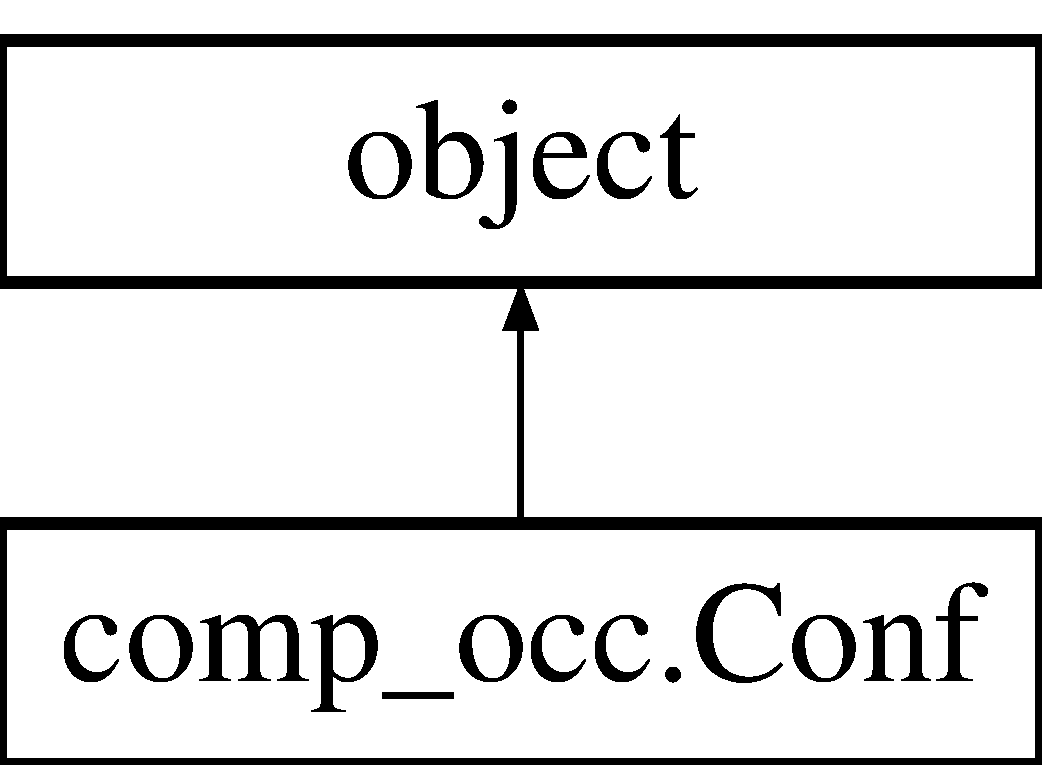
\includegraphics[height=2.000000cm]{classcomp__occ_1_1_conf}
\end{center}
\end{figure}
\subsection*{Public Member Functions}
\begin{DoxyCompactItemize}
\item 
def \hyperlink{classcomp__occ_1_1_conf_a8bcfb9626fe1990cd68bb3701a36fb5f}{\-\_\-\-\_\-init\-\_\-\-\_\-}
\end{DoxyCompactItemize}
\subsection*{Public Attributes}
\begin{DoxyCompactItemize}
\item 
\hyperlink{classcomp__occ_1_1_conf_ac424346df2bb8a9b7548c6c5768633a4}{conf\-Name}
\item 
\hyperlink{classcomp__occ_1_1_conf_a6b6a4ed6f56d67c757fe8851386fd674}{occ}
\end{DoxyCompactItemize}


\subsection{Detailed Description}
Compare the occupancy of conformers in two different runs. 

Conformer class. 

\subsection{Constructor \& Destructor Documentation}
\hypertarget{classcomp__occ_1_1_conf_a8bcfb9626fe1990cd68bb3701a36fb5f}{\index{comp\-\_\-occ\-::\-Conf@{comp\-\_\-occ\-::\-Conf}!\-\_\-\-\_\-init\-\_\-\-\_\-@{\-\_\-\-\_\-init\-\_\-\-\_\-}}
\index{\-\_\-\-\_\-init\-\_\-\-\_\-@{\-\_\-\-\_\-init\-\_\-\-\_\-}!comp_occ::Conf@{comp\-\_\-occ\-::\-Conf}}
\subsubsection[{\-\_\-\-\_\-init\-\_\-\-\_\-}]{\setlength{\rightskip}{0pt plus 5cm}def comp\-\_\-occ.\-Conf.\-\_\-\-\_\-init\-\_\-\-\_\- (
\begin{DoxyParamCaption}
\item[{}]{self, }
\item[{}]{res\-Name = {\ttfamily \char`\"{}\char`\"{}}, }
\item[{}]{occ = {\ttfamily 0.0}}
\end{DoxyParamCaption}
)}}\label{classcomp__occ_1_1_conf_a8bcfb9626fe1990cd68bb3701a36fb5f}


\subsection{Member Data Documentation}
\hypertarget{classcomp__occ_1_1_conf_ac424346df2bb8a9b7548c6c5768633a4}{\index{comp\-\_\-occ\-::\-Conf@{comp\-\_\-occ\-::\-Conf}!conf\-Name@{conf\-Name}}
\index{conf\-Name@{conf\-Name}!comp_occ::Conf@{comp\-\_\-occ\-::\-Conf}}
\subsubsection[{conf\-Name}]{\setlength{\rightskip}{0pt plus 5cm}comp\-\_\-occ.\-Conf.\-conf\-Name}}\label{classcomp__occ_1_1_conf_ac424346df2bb8a9b7548c6c5768633a4}
\hypertarget{classcomp__occ_1_1_conf_a6b6a4ed6f56d67c757fe8851386fd674}{\index{comp\-\_\-occ\-::\-Conf@{comp\-\_\-occ\-::\-Conf}!occ@{occ}}
\index{occ@{occ}!comp_occ::Conf@{comp\-\_\-occ\-::\-Conf}}
\subsubsection[{occ}]{\setlength{\rightskip}{0pt plus 5cm}comp\-\_\-occ.\-Conf.\-occ}}\label{classcomp__occ_1_1_conf_a6b6a4ed6f56d67c757fe8851386fd674}


The documentation for this class was generated from the following file\-:\begin{DoxyCompactItemize}
\item 
src/scripts/mcce/\hyperlink{comp__occ_8py}{comp\-\_\-occ.\-py}\end{DoxyCompactItemize}

\hypertarget{classmocc_1_1_conf}{\section{mocc.\-Conf Class Reference}
\label{classmocc_1_1_conf}\index{mocc.\-Conf@{mocc.\-Conf}}
}


Conformer class.  


Inheritance diagram for mocc.\-Conf\-:\begin{figure}[H]
\begin{center}
\leavevmode
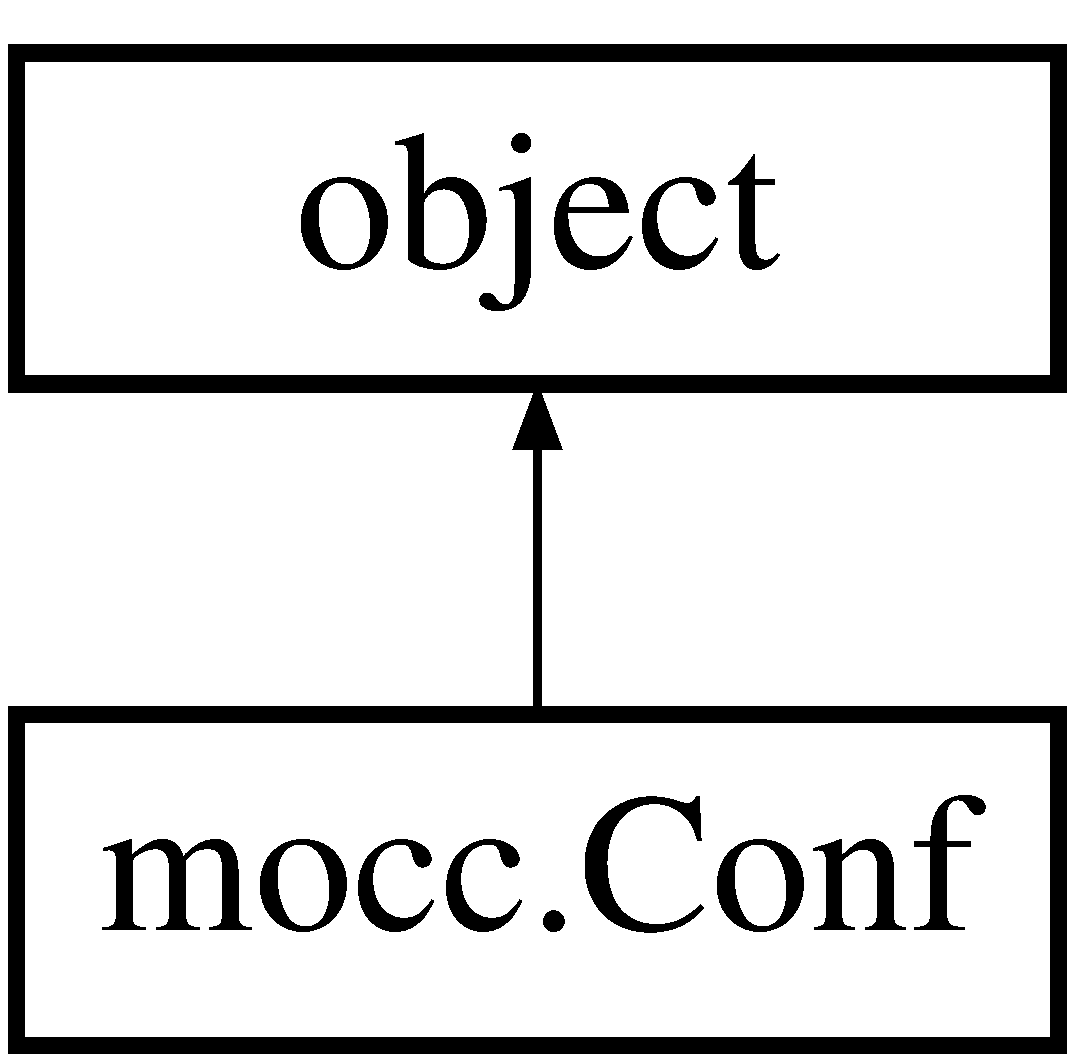
\includegraphics[height=2.000000cm]{classmocc_1_1_conf}
\end{center}
\end{figure}
\subsection*{Public Member Functions}
\begin{DoxyCompactItemize}
\item 
def \hyperlink{classmocc_1_1_conf_aa500603293a8484e5a5be6b8c464aea2}{\-\_\-\-\_\-init\-\_\-\-\_\-}
\item 
def \hyperlink{classmocc_1_1_conf_acd95b13da7989dcab1ae34694c4a1869}{load\-\_\-s2}
\begin{DoxyCompactList}\small\item\em Load the info of the conformer from a line in \char`\"{}step2\-\_\-out.\-pdb\char`\"{}. \end{DoxyCompactList}\item 
def \hyperlink{classmocc_1_1_conf_a70483b8650a6ea020699a2aeeeb8bc8b}{write\-\_\-pdb}
\begin{DoxyCompactList}\small\item\em Write the conformer to a pdb file. \end{DoxyCompactList}\end{DoxyCompactItemize}
\subsection*{Public Attributes}
\begin{DoxyCompactItemize}
\item 
\hyperlink{classmocc_1_1_conf_aca1ad7dd1cbd3016b49d0324cd215a6c}{confid}
\item 
\hyperlink{classmocc_1_1_conf_a502e54dae7949b03753996d86fa00ec3}{occ}
\item 
\hyperlink{classmocc_1_1_conf_afb6520f03e8170fa7f13806ad6960b1e}{resid}
\item 
\hyperlink{classmocc_1_1_conf_a4d4f705ae22c4a96a17a63cfa5dbc51d}{chainid}
\item 
\hyperlink{classmocc_1_1_conf_a9b80e40b5c8f4ee88bb5c3c0e8864055}{resseq}
\item 
\hyperlink{classmocc_1_1_conf_a1a614c66d33ebd31d4f1493c90ca5ff5}{x2}
\item 
\hyperlink{classmocc_1_1_conf_a1bd6811ef470dd12245b214c639c50d5}{s\-\_\-head}
\item 
\hyperlink{classmocc_1_1_conf_abe64fbfee389298b7ab826e203c3684b}{cor}
\end{DoxyCompactItemize}


\subsection{Detailed Description}
Conformer class. 

\subsection{Constructor \& Destructor Documentation}
\hypertarget{classmocc_1_1_conf_aa500603293a8484e5a5be6b8c464aea2}{\index{mocc\-::\-Conf@{mocc\-::\-Conf}!\-\_\-\-\_\-init\-\_\-\-\_\-@{\-\_\-\-\_\-init\-\_\-\-\_\-}}
\index{\-\_\-\-\_\-init\-\_\-\-\_\-@{\-\_\-\-\_\-init\-\_\-\-\_\-}!mocc::Conf@{mocc\-::\-Conf}}
\subsubsection[{\-\_\-\-\_\-init\-\_\-\-\_\-}]{\setlength{\rightskip}{0pt plus 5cm}def mocc.\-Conf.\-\_\-\-\_\-init\-\_\-\-\_\- (
\begin{DoxyParamCaption}
\item[{}]{self, }
\item[{}]{f\-\_\-line, }
\item[{}]{t\-\_\-col}
\end{DoxyParamCaption}
)}}\label{classmocc_1_1_conf_aa500603293a8484e5a5be6b8c464aea2}


\subsection{Member Function Documentation}
\hypertarget{classmocc_1_1_conf_acd95b13da7989dcab1ae34694c4a1869}{\index{mocc\-::\-Conf@{mocc\-::\-Conf}!load\-\_\-s2@{load\-\_\-s2}}
\index{load\-\_\-s2@{load\-\_\-s2}!mocc::Conf@{mocc\-::\-Conf}}
\subsubsection[{load\-\_\-s2}]{\setlength{\rightskip}{0pt plus 5cm}def mocc.\-Conf.\-load\-\_\-s2 (
\begin{DoxyParamCaption}
\item[{}]{self, }
\item[{}]{s\-\_\-line}
\end{DoxyParamCaption}
)}}\label{classmocc_1_1_conf_acd95b13da7989dcab1ae34694c4a1869}


Load the info of the conformer from a line in \char`\"{}step2\-\_\-out.\-pdb\char`\"{}. 

One atom of the conformer is loaded. \hypertarget{classmocc_1_1_conf_a70483b8650a6ea020699a2aeeeb8bc8b}{\index{mocc\-::\-Conf@{mocc\-::\-Conf}!write\-\_\-pdb@{write\-\_\-pdb}}
\index{write\-\_\-pdb@{write\-\_\-pdb}!mocc::Conf@{mocc\-::\-Conf}}
\subsubsection[{write\-\_\-pdb}]{\setlength{\rightskip}{0pt plus 5cm}def mocc.\-Conf.\-write\-\_\-pdb (
\begin{DoxyParamCaption}
\item[{}]{self, }
\item[{}]{fp}
\end{DoxyParamCaption}
)}}\label{classmocc_1_1_conf_a70483b8650a6ea020699a2aeeeb8bc8b}


Write the conformer to a pdb file. 

All the atoms of this conformer need to be written. 

\subsection{Member Data Documentation}
\hypertarget{classmocc_1_1_conf_a4d4f705ae22c4a96a17a63cfa5dbc51d}{\index{mocc\-::\-Conf@{mocc\-::\-Conf}!chainid@{chainid}}
\index{chainid@{chainid}!mocc::Conf@{mocc\-::\-Conf}}
\subsubsection[{chainid}]{\setlength{\rightskip}{0pt plus 5cm}mocc.\-Conf.\-chainid}}\label{classmocc_1_1_conf_a4d4f705ae22c4a96a17a63cfa5dbc51d}
\hypertarget{classmocc_1_1_conf_aca1ad7dd1cbd3016b49d0324cd215a6c}{\index{mocc\-::\-Conf@{mocc\-::\-Conf}!confid@{confid}}
\index{confid@{confid}!mocc::Conf@{mocc\-::\-Conf}}
\subsubsection[{confid}]{\setlength{\rightskip}{0pt plus 5cm}mocc.\-Conf.\-confid}}\label{classmocc_1_1_conf_aca1ad7dd1cbd3016b49d0324cd215a6c}
\hypertarget{classmocc_1_1_conf_abe64fbfee389298b7ab826e203c3684b}{\index{mocc\-::\-Conf@{mocc\-::\-Conf}!cor@{cor}}
\index{cor@{cor}!mocc::Conf@{mocc\-::\-Conf}}
\subsubsection[{cor}]{\setlength{\rightskip}{0pt plus 5cm}mocc.\-Conf.\-cor}}\label{classmocc_1_1_conf_abe64fbfee389298b7ab826e203c3684b}
\hypertarget{classmocc_1_1_conf_a502e54dae7949b03753996d86fa00ec3}{\index{mocc\-::\-Conf@{mocc\-::\-Conf}!occ@{occ}}
\index{occ@{occ}!mocc::Conf@{mocc\-::\-Conf}}
\subsubsection[{occ}]{\setlength{\rightskip}{0pt plus 5cm}mocc.\-Conf.\-occ}}\label{classmocc_1_1_conf_a502e54dae7949b03753996d86fa00ec3}
\hypertarget{classmocc_1_1_conf_afb6520f03e8170fa7f13806ad6960b1e}{\index{mocc\-::\-Conf@{mocc\-::\-Conf}!resid@{resid}}
\index{resid@{resid}!mocc::Conf@{mocc\-::\-Conf}}
\subsubsection[{resid}]{\setlength{\rightskip}{0pt plus 5cm}mocc.\-Conf.\-resid}}\label{classmocc_1_1_conf_afb6520f03e8170fa7f13806ad6960b1e}
\hypertarget{classmocc_1_1_conf_a9b80e40b5c8f4ee88bb5c3c0e8864055}{\index{mocc\-::\-Conf@{mocc\-::\-Conf}!resseq@{resseq}}
\index{resseq@{resseq}!mocc::Conf@{mocc\-::\-Conf}}
\subsubsection[{resseq}]{\setlength{\rightskip}{0pt plus 5cm}mocc.\-Conf.\-resseq}}\label{classmocc_1_1_conf_a9b80e40b5c8f4ee88bb5c3c0e8864055}
\hypertarget{classmocc_1_1_conf_a1bd6811ef470dd12245b214c639c50d5}{\index{mocc\-::\-Conf@{mocc\-::\-Conf}!s\-\_\-head@{s\-\_\-head}}
\index{s\-\_\-head@{s\-\_\-head}!mocc::Conf@{mocc\-::\-Conf}}
\subsubsection[{s\-\_\-head}]{\setlength{\rightskip}{0pt plus 5cm}mocc.\-Conf.\-s\-\_\-head}}\label{classmocc_1_1_conf_a1bd6811ef470dd12245b214c639c50d5}
\hypertarget{classmocc_1_1_conf_a1a614c66d33ebd31d4f1493c90ca5ff5}{\index{mocc\-::\-Conf@{mocc\-::\-Conf}!x2@{x2}}
\index{x2@{x2}!mocc::Conf@{mocc\-::\-Conf}}
\subsubsection[{x2}]{\setlength{\rightskip}{0pt plus 5cm}mocc.\-Conf.\-x2}}\label{classmocc_1_1_conf_a1a614c66d33ebd31d4f1493c90ca5ff5}


The documentation for this class was generated from the following file\-:\begin{DoxyCompactItemize}
\item 
src/scripts/mcce/\hyperlink{mocc_8py}{mocc.\-py}\end{DoxyCompactItemize}

\hypertarget{classxmccepy_1_1mp_1_1_c_o_n_f_o_r_m_e_r}{\section{xmccepy.\-mp.\-C\-O\-N\-F\-O\-R\-M\-E\-R Class Reference}
\label{classxmccepy_1_1mp_1_1_c_o_n_f_o_r_m_e_r}\index{xmccepy.\-mp.\-C\-O\-N\-F\-O\-R\-M\-E\-R@{xmccepy.\-mp.\-C\-O\-N\-F\-O\-R\-M\-E\-R}}
}
\subsection*{Public Member Functions}
\begin{DoxyCompactItemize}
\item 
def \hyperlink{classxmccepy_1_1mp_1_1_c_o_n_f_o_r_m_e_r_a371854582bd48c21b894a085ec7a9ee4}{\-\_\-\-\_\-init\-\_\-\-\_\-}
\item 
def \hyperlink{classxmccepy_1_1mp_1_1_c_o_n_f_o_r_m_e_r_a2045e40a7a38d8b544c57602d96d25e5}{initial\-\_\-by\-\_\-h3}
\item 
def \hyperlink{classxmccepy_1_1mp_1_1_c_o_n_f_o_r_m_e_r_a0c0b2d9ce8d8fb9e60edf81e618f082e}{in\-Res}
\item 
def \hyperlink{classxmccepy_1_1mp_1_1_c_o_n_f_o_r_m_e_r_a0cce02a0def0a04375125568491cc635}{load\-\_\-occ}
\end{DoxyCompactItemize}
\subsection*{Public Attributes}
\begin{DoxyCompactItemize}
\item 
\hyperlink{classxmccepy_1_1mp_1_1_c_o_n_f_o_r_m_e_r_a6a748e760bc097c1560578f42a9f857f}{atoms}
\item 
\hyperlink{classxmccepy_1_1mp_1_1_c_o_n_f_o_r_m_e_r_a9e5bf147326267319ff6e530c6fe2184}{res\-Name}
\item 
\hyperlink{classxmccepy_1_1mp_1_1_c_o_n_f_o_r_m_e_r_abd94248291d7e1014b784a61572b9b56}{res\-Seq}
\item 
\hyperlink{classxmccepy_1_1mp_1_1_c_o_n_f_o_r_m_e_r_a7200c512bdf3481f4244005873802833}{conf\-Name}
\item 
\hyperlink{classxmccepy_1_1mp_1_1_c_o_n_f_o_r_m_e_r_afc8af5d1e1ca01bc54162eef3076c0e7}{i\-Code}
\item 
\hyperlink{classxmccepy_1_1mp_1_1_c_o_n_f_o_r_m_e_r_a5e08044df96e2efc98d27d11dad2acc0}{i\-Conf}
\item 
\hyperlink{classxmccepy_1_1mp_1_1_c_o_n_f_o_r_m_e_r_a80e8729d25aa77487916dfc0b0be6c7d}{crg}
\item 
\hyperlink{classxmccepy_1_1mp_1_1_c_o_n_f_o_r_m_e_r_a62ff7372f23a1c40ea1967aaffad993c}{Em0}
\item 
\hyperlink{classxmccepy_1_1mp_1_1_c_o_n_f_o_r_m_e_r_a6b1bf83b15461d60baa91de328d195ce}{p\-Ka0}
\item 
\hyperlink{classxmccepy_1_1mp_1_1_c_o_n_f_o_r_m_e_r_ab0377ce0611af60ca84fa253d32289ca}{ne}
\item 
\hyperlink{classxmccepy_1_1mp_1_1_c_o_n_f_o_r_m_e_r_aef85f7fcfb8665f154e0fad915dbac5e}{n\-H}
\item 
\hyperlink{classxmccepy_1_1mp_1_1_c_o_n_f_o_r_m_e_r_a54266cbd09ba1b62ac724a688a077623}{F\-L}
\item 
\hyperlink{classxmccepy_1_1mp_1_1_c_o_n_f_o_r_m_e_r_aaf6ca8e069b34e52bfb9f5e95c24b859}{occ}
\item 
\hyperlink{classxmccepy_1_1mp_1_1_c_o_n_f_o_r_m_e_r_a6d2a83a118c9117dc938e954e7e5cac6}{E\-\_\-vdw0}
\item 
\hyperlink{classxmccepy_1_1mp_1_1_c_o_n_f_o_r_m_e_r_ae98aded8558a5101a760bb9b60101bac}{E\-\_\-vdw1}
\item 
\hyperlink{classxmccepy_1_1mp_1_1_c_o_n_f_o_r_m_e_r_a442b37096eecb715ef0637298e647a27}{E\-\_\-tors}
\item 
\hyperlink{classxmccepy_1_1mp_1_1_c_o_n_f_o_r_m_e_r_ab3a58e71ca1eff5c19a49c3e7ed4c682}{E\-\_\-epol}
\item 
\hyperlink{classxmccepy_1_1mp_1_1_c_o_n_f_o_r_m_e_r_a05f3e253b3e75d0868f55babb6d39d61}{E\-\_\-dsolv}
\item 
\hyperlink{classxmccepy_1_1mp_1_1_c_o_n_f_o_r_m_e_r_abd6de497b74afb9d65545f1581a2b88d}{extra}
\item 
\hyperlink{classxmccepy_1_1mp_1_1_c_o_n_f_o_r_m_e_r_a78d0c3efc8bbf322e759a475e7eb74e0}{history}
\item 
\hyperlink{classxmccepy_1_1mp_1_1_c_o_n_f_o_r_m_e_r_ac1880aa3dad24483cb41a4bf5da0c640}{focc}
\item 
\hyperlink{classxmccepy_1_1mp_1_1_c_o_n_f_o_r_m_e_r_a32f981febbee2d7b5e6e9099f1ced82c}{E\-\_\-extra}
\end{DoxyCompactItemize}


\subsection{Constructor \& Destructor Documentation}
\hypertarget{classxmccepy_1_1mp_1_1_c_o_n_f_o_r_m_e_r_a371854582bd48c21b894a085ec7a9ee4}{\index{xmccepy\-::mp\-::\-C\-O\-N\-F\-O\-R\-M\-E\-R@{xmccepy\-::mp\-::\-C\-O\-N\-F\-O\-R\-M\-E\-R}!\-\_\-\-\_\-init\-\_\-\-\_\-@{\-\_\-\-\_\-init\-\_\-\-\_\-}}
\index{\-\_\-\-\_\-init\-\_\-\-\_\-@{\-\_\-\-\_\-init\-\_\-\-\_\-}!xmccepy::mp::CONFORMER@{xmccepy\-::mp\-::\-C\-O\-N\-F\-O\-R\-M\-E\-R}}
\subsubsection[{\-\_\-\-\_\-init\-\_\-\-\_\-}]{\setlength{\rightskip}{0pt plus 5cm}def xmccepy.\-mp.\-C\-O\-N\-F\-O\-R\-M\-E\-R.\-\_\-\-\_\-init\-\_\-\-\_\- (
\begin{DoxyParamCaption}
\item[{}]{self}
\end{DoxyParamCaption}
)}}\label{classxmccepy_1_1mp_1_1_c_o_n_f_o_r_m_e_r_a371854582bd48c21b894a085ec7a9ee4}


\subsection{Member Function Documentation}
\hypertarget{classxmccepy_1_1mp_1_1_c_o_n_f_o_r_m_e_r_a2045e40a7a38d8b544c57602d96d25e5}{\index{xmccepy\-::mp\-::\-C\-O\-N\-F\-O\-R\-M\-E\-R@{xmccepy\-::mp\-::\-C\-O\-N\-F\-O\-R\-M\-E\-R}!initial\-\_\-by\-\_\-h3@{initial\-\_\-by\-\_\-h3}}
\index{initial\-\_\-by\-\_\-h3@{initial\-\_\-by\-\_\-h3}!xmccepy::mp::CONFORMER@{xmccepy\-::mp\-::\-C\-O\-N\-F\-O\-R\-M\-E\-R}}
\subsubsection[{initial\-\_\-by\-\_\-h3}]{\setlength{\rightskip}{0pt plus 5cm}def xmccepy.\-mp.\-C\-O\-N\-F\-O\-R\-M\-E\-R.\-initial\-\_\-by\-\_\-h3 (
\begin{DoxyParamCaption}
\item[{}]{line}
\end{DoxyParamCaption}
)}}\label{classxmccepy_1_1mp_1_1_c_o_n_f_o_r_m_e_r_a2045e40a7a38d8b544c57602d96d25e5}
\hypertarget{classxmccepy_1_1mp_1_1_c_o_n_f_o_r_m_e_r_a0c0b2d9ce8d8fb9e60edf81e618f082e}{\index{xmccepy\-::mp\-::\-C\-O\-N\-F\-O\-R\-M\-E\-R@{xmccepy\-::mp\-::\-C\-O\-N\-F\-O\-R\-M\-E\-R}!in\-Res@{in\-Res}}
\index{in\-Res@{in\-Res}!xmccepy::mp::CONFORMER@{xmccepy\-::mp\-::\-C\-O\-N\-F\-O\-R\-M\-E\-R}}
\subsubsection[{in\-Res}]{\setlength{\rightskip}{0pt plus 5cm}def xmccepy.\-mp.\-C\-O\-N\-F\-O\-R\-M\-E\-R.\-in\-Res (
\begin{DoxyParamCaption}
\item[{}]{res\-Name}
\end{DoxyParamCaption}
)}}\label{classxmccepy_1_1mp_1_1_c_o_n_f_o_r_m_e_r_a0c0b2d9ce8d8fb9e60edf81e618f082e}
\hypertarget{classxmccepy_1_1mp_1_1_c_o_n_f_o_r_m_e_r_a0cce02a0def0a04375125568491cc635}{\index{xmccepy\-::mp\-::\-C\-O\-N\-F\-O\-R\-M\-E\-R@{xmccepy\-::mp\-::\-C\-O\-N\-F\-O\-R\-M\-E\-R}!load\-\_\-occ@{load\-\_\-occ}}
\index{load\-\_\-occ@{load\-\_\-occ}!xmccepy::mp::CONFORMER@{xmccepy\-::mp\-::\-C\-O\-N\-F\-O\-R\-M\-E\-R}}
\subsubsection[{load\-\_\-occ}]{\setlength{\rightskip}{0pt plus 5cm}def xmccepy.\-mp.\-C\-O\-N\-F\-O\-R\-M\-E\-R.\-load\-\_\-occ (
\begin{DoxyParamCaption}
\item[{}]{line}
\end{DoxyParamCaption}
)}}\label{classxmccepy_1_1mp_1_1_c_o_n_f_o_r_m_e_r_a0cce02a0def0a04375125568491cc635}


\subsection{Member Data Documentation}
\hypertarget{classxmccepy_1_1mp_1_1_c_o_n_f_o_r_m_e_r_a6a748e760bc097c1560578f42a9f857f}{\index{xmccepy\-::mp\-::\-C\-O\-N\-F\-O\-R\-M\-E\-R@{xmccepy\-::mp\-::\-C\-O\-N\-F\-O\-R\-M\-E\-R}!atoms@{atoms}}
\index{atoms@{atoms}!xmccepy::mp::CONFORMER@{xmccepy\-::mp\-::\-C\-O\-N\-F\-O\-R\-M\-E\-R}}
\subsubsection[{atoms}]{\setlength{\rightskip}{0pt plus 5cm}xmccepy.\-mp.\-C\-O\-N\-F\-O\-R\-M\-E\-R.\-atoms}}\label{classxmccepy_1_1mp_1_1_c_o_n_f_o_r_m_e_r_a6a748e760bc097c1560578f42a9f857f}
\hypertarget{classxmccepy_1_1mp_1_1_c_o_n_f_o_r_m_e_r_a7200c512bdf3481f4244005873802833}{\index{xmccepy\-::mp\-::\-C\-O\-N\-F\-O\-R\-M\-E\-R@{xmccepy\-::mp\-::\-C\-O\-N\-F\-O\-R\-M\-E\-R}!conf\-Name@{conf\-Name}}
\index{conf\-Name@{conf\-Name}!xmccepy::mp::CONFORMER@{xmccepy\-::mp\-::\-C\-O\-N\-F\-O\-R\-M\-E\-R}}
\subsubsection[{conf\-Name}]{\setlength{\rightskip}{0pt plus 5cm}xmccepy.\-mp.\-C\-O\-N\-F\-O\-R\-M\-E\-R.\-conf\-Name}}\label{classxmccepy_1_1mp_1_1_c_o_n_f_o_r_m_e_r_a7200c512bdf3481f4244005873802833}
\hypertarget{classxmccepy_1_1mp_1_1_c_o_n_f_o_r_m_e_r_a80e8729d25aa77487916dfc0b0be6c7d}{\index{xmccepy\-::mp\-::\-C\-O\-N\-F\-O\-R\-M\-E\-R@{xmccepy\-::mp\-::\-C\-O\-N\-F\-O\-R\-M\-E\-R}!crg@{crg}}
\index{crg@{crg}!xmccepy::mp::CONFORMER@{xmccepy\-::mp\-::\-C\-O\-N\-F\-O\-R\-M\-E\-R}}
\subsubsection[{crg}]{\setlength{\rightskip}{0pt plus 5cm}xmccepy.\-mp.\-C\-O\-N\-F\-O\-R\-M\-E\-R.\-crg}}\label{classxmccepy_1_1mp_1_1_c_o_n_f_o_r_m_e_r_a80e8729d25aa77487916dfc0b0be6c7d}
\hypertarget{classxmccepy_1_1mp_1_1_c_o_n_f_o_r_m_e_r_a05f3e253b3e75d0868f55babb6d39d61}{\index{xmccepy\-::mp\-::\-C\-O\-N\-F\-O\-R\-M\-E\-R@{xmccepy\-::mp\-::\-C\-O\-N\-F\-O\-R\-M\-E\-R}!E\-\_\-dsolv@{E\-\_\-dsolv}}
\index{E\-\_\-dsolv@{E\-\_\-dsolv}!xmccepy::mp::CONFORMER@{xmccepy\-::mp\-::\-C\-O\-N\-F\-O\-R\-M\-E\-R}}
\subsubsection[{E\-\_\-dsolv}]{\setlength{\rightskip}{0pt plus 5cm}xmccepy.\-mp.\-C\-O\-N\-F\-O\-R\-M\-E\-R.\-E\-\_\-dsolv}}\label{classxmccepy_1_1mp_1_1_c_o_n_f_o_r_m_e_r_a05f3e253b3e75d0868f55babb6d39d61}
\hypertarget{classxmccepy_1_1mp_1_1_c_o_n_f_o_r_m_e_r_ab3a58e71ca1eff5c19a49c3e7ed4c682}{\index{xmccepy\-::mp\-::\-C\-O\-N\-F\-O\-R\-M\-E\-R@{xmccepy\-::mp\-::\-C\-O\-N\-F\-O\-R\-M\-E\-R}!E\-\_\-epol@{E\-\_\-epol}}
\index{E\-\_\-epol@{E\-\_\-epol}!xmccepy::mp::CONFORMER@{xmccepy\-::mp\-::\-C\-O\-N\-F\-O\-R\-M\-E\-R}}
\subsubsection[{E\-\_\-epol}]{\setlength{\rightskip}{0pt plus 5cm}xmccepy.\-mp.\-C\-O\-N\-F\-O\-R\-M\-E\-R.\-E\-\_\-epol}}\label{classxmccepy_1_1mp_1_1_c_o_n_f_o_r_m_e_r_ab3a58e71ca1eff5c19a49c3e7ed4c682}
\hypertarget{classxmccepy_1_1mp_1_1_c_o_n_f_o_r_m_e_r_a32f981febbee2d7b5e6e9099f1ced82c}{\index{xmccepy\-::mp\-::\-C\-O\-N\-F\-O\-R\-M\-E\-R@{xmccepy\-::mp\-::\-C\-O\-N\-F\-O\-R\-M\-E\-R}!E\-\_\-extra@{E\-\_\-extra}}
\index{E\-\_\-extra@{E\-\_\-extra}!xmccepy::mp::CONFORMER@{xmccepy\-::mp\-::\-C\-O\-N\-F\-O\-R\-M\-E\-R}}
\subsubsection[{E\-\_\-extra}]{\setlength{\rightskip}{0pt plus 5cm}xmccepy.\-mp.\-C\-O\-N\-F\-O\-R\-M\-E\-R.\-E\-\_\-extra}}\label{classxmccepy_1_1mp_1_1_c_o_n_f_o_r_m_e_r_a32f981febbee2d7b5e6e9099f1ced82c}
\hypertarget{classxmccepy_1_1mp_1_1_c_o_n_f_o_r_m_e_r_a442b37096eecb715ef0637298e647a27}{\index{xmccepy\-::mp\-::\-C\-O\-N\-F\-O\-R\-M\-E\-R@{xmccepy\-::mp\-::\-C\-O\-N\-F\-O\-R\-M\-E\-R}!E\-\_\-tors@{E\-\_\-tors}}
\index{E\-\_\-tors@{E\-\_\-tors}!xmccepy::mp::CONFORMER@{xmccepy\-::mp\-::\-C\-O\-N\-F\-O\-R\-M\-E\-R}}
\subsubsection[{E\-\_\-tors}]{\setlength{\rightskip}{0pt plus 5cm}xmccepy.\-mp.\-C\-O\-N\-F\-O\-R\-M\-E\-R.\-E\-\_\-tors}}\label{classxmccepy_1_1mp_1_1_c_o_n_f_o_r_m_e_r_a442b37096eecb715ef0637298e647a27}
\hypertarget{classxmccepy_1_1mp_1_1_c_o_n_f_o_r_m_e_r_a6d2a83a118c9117dc938e954e7e5cac6}{\index{xmccepy\-::mp\-::\-C\-O\-N\-F\-O\-R\-M\-E\-R@{xmccepy\-::mp\-::\-C\-O\-N\-F\-O\-R\-M\-E\-R}!E\-\_\-vdw0@{E\-\_\-vdw0}}
\index{E\-\_\-vdw0@{E\-\_\-vdw0}!xmccepy::mp::CONFORMER@{xmccepy\-::mp\-::\-C\-O\-N\-F\-O\-R\-M\-E\-R}}
\subsubsection[{E\-\_\-vdw0}]{\setlength{\rightskip}{0pt plus 5cm}xmccepy.\-mp.\-C\-O\-N\-F\-O\-R\-M\-E\-R.\-E\-\_\-vdw0}}\label{classxmccepy_1_1mp_1_1_c_o_n_f_o_r_m_e_r_a6d2a83a118c9117dc938e954e7e5cac6}
\hypertarget{classxmccepy_1_1mp_1_1_c_o_n_f_o_r_m_e_r_ae98aded8558a5101a760bb9b60101bac}{\index{xmccepy\-::mp\-::\-C\-O\-N\-F\-O\-R\-M\-E\-R@{xmccepy\-::mp\-::\-C\-O\-N\-F\-O\-R\-M\-E\-R}!E\-\_\-vdw1@{E\-\_\-vdw1}}
\index{E\-\_\-vdw1@{E\-\_\-vdw1}!xmccepy::mp::CONFORMER@{xmccepy\-::mp\-::\-C\-O\-N\-F\-O\-R\-M\-E\-R}}
\subsubsection[{E\-\_\-vdw1}]{\setlength{\rightskip}{0pt plus 5cm}xmccepy.\-mp.\-C\-O\-N\-F\-O\-R\-M\-E\-R.\-E\-\_\-vdw1}}\label{classxmccepy_1_1mp_1_1_c_o_n_f_o_r_m_e_r_ae98aded8558a5101a760bb9b60101bac}
\hypertarget{classxmccepy_1_1mp_1_1_c_o_n_f_o_r_m_e_r_a62ff7372f23a1c40ea1967aaffad993c}{\index{xmccepy\-::mp\-::\-C\-O\-N\-F\-O\-R\-M\-E\-R@{xmccepy\-::mp\-::\-C\-O\-N\-F\-O\-R\-M\-E\-R}!Em0@{Em0}}
\index{Em0@{Em0}!xmccepy::mp::CONFORMER@{xmccepy\-::mp\-::\-C\-O\-N\-F\-O\-R\-M\-E\-R}}
\subsubsection[{Em0}]{\setlength{\rightskip}{0pt plus 5cm}xmccepy.\-mp.\-C\-O\-N\-F\-O\-R\-M\-E\-R.\-Em0}}\label{classxmccepy_1_1mp_1_1_c_o_n_f_o_r_m_e_r_a62ff7372f23a1c40ea1967aaffad993c}
\hypertarget{classxmccepy_1_1mp_1_1_c_o_n_f_o_r_m_e_r_abd6de497b74afb9d65545f1581a2b88d}{\index{xmccepy\-::mp\-::\-C\-O\-N\-F\-O\-R\-M\-E\-R@{xmccepy\-::mp\-::\-C\-O\-N\-F\-O\-R\-M\-E\-R}!extra@{extra}}
\index{extra@{extra}!xmccepy::mp::CONFORMER@{xmccepy\-::mp\-::\-C\-O\-N\-F\-O\-R\-M\-E\-R}}
\subsubsection[{extra}]{\setlength{\rightskip}{0pt plus 5cm}xmccepy.\-mp.\-C\-O\-N\-F\-O\-R\-M\-E\-R.\-extra}}\label{classxmccepy_1_1mp_1_1_c_o_n_f_o_r_m_e_r_abd6de497b74afb9d65545f1581a2b88d}
\hypertarget{classxmccepy_1_1mp_1_1_c_o_n_f_o_r_m_e_r_a54266cbd09ba1b62ac724a688a077623}{\index{xmccepy\-::mp\-::\-C\-O\-N\-F\-O\-R\-M\-E\-R@{xmccepy\-::mp\-::\-C\-O\-N\-F\-O\-R\-M\-E\-R}!F\-L@{F\-L}}
\index{F\-L@{F\-L}!xmccepy::mp::CONFORMER@{xmccepy\-::mp\-::\-C\-O\-N\-F\-O\-R\-M\-E\-R}}
\subsubsection[{F\-L}]{\setlength{\rightskip}{0pt plus 5cm}xmccepy.\-mp.\-C\-O\-N\-F\-O\-R\-M\-E\-R.\-F\-L}}\label{classxmccepy_1_1mp_1_1_c_o_n_f_o_r_m_e_r_a54266cbd09ba1b62ac724a688a077623}
\hypertarget{classxmccepy_1_1mp_1_1_c_o_n_f_o_r_m_e_r_ac1880aa3dad24483cb41a4bf5da0c640}{\index{xmccepy\-::mp\-::\-C\-O\-N\-F\-O\-R\-M\-E\-R@{xmccepy\-::mp\-::\-C\-O\-N\-F\-O\-R\-M\-E\-R}!focc@{focc}}
\index{focc@{focc}!xmccepy::mp::CONFORMER@{xmccepy\-::mp\-::\-C\-O\-N\-F\-O\-R\-M\-E\-R}}
\subsubsection[{focc}]{\setlength{\rightskip}{0pt plus 5cm}xmccepy.\-mp.\-C\-O\-N\-F\-O\-R\-M\-E\-R.\-focc}}\label{classxmccepy_1_1mp_1_1_c_o_n_f_o_r_m_e_r_ac1880aa3dad24483cb41a4bf5da0c640}
\hypertarget{classxmccepy_1_1mp_1_1_c_o_n_f_o_r_m_e_r_a78d0c3efc8bbf322e759a475e7eb74e0}{\index{xmccepy\-::mp\-::\-C\-O\-N\-F\-O\-R\-M\-E\-R@{xmccepy\-::mp\-::\-C\-O\-N\-F\-O\-R\-M\-E\-R}!history@{history}}
\index{history@{history}!xmccepy::mp::CONFORMER@{xmccepy\-::mp\-::\-C\-O\-N\-F\-O\-R\-M\-E\-R}}
\subsubsection[{history}]{\setlength{\rightskip}{0pt plus 5cm}xmccepy.\-mp.\-C\-O\-N\-F\-O\-R\-M\-E\-R.\-history}}\label{classxmccepy_1_1mp_1_1_c_o_n_f_o_r_m_e_r_a78d0c3efc8bbf322e759a475e7eb74e0}
\hypertarget{classxmccepy_1_1mp_1_1_c_o_n_f_o_r_m_e_r_afc8af5d1e1ca01bc54162eef3076c0e7}{\index{xmccepy\-::mp\-::\-C\-O\-N\-F\-O\-R\-M\-E\-R@{xmccepy\-::mp\-::\-C\-O\-N\-F\-O\-R\-M\-E\-R}!i\-Code@{i\-Code}}
\index{i\-Code@{i\-Code}!xmccepy::mp::CONFORMER@{xmccepy\-::mp\-::\-C\-O\-N\-F\-O\-R\-M\-E\-R}}
\subsubsection[{i\-Code}]{\setlength{\rightskip}{0pt plus 5cm}xmccepy.\-mp.\-C\-O\-N\-F\-O\-R\-M\-E\-R.\-i\-Code}}\label{classxmccepy_1_1mp_1_1_c_o_n_f_o_r_m_e_r_afc8af5d1e1ca01bc54162eef3076c0e7}
\hypertarget{classxmccepy_1_1mp_1_1_c_o_n_f_o_r_m_e_r_a5e08044df96e2efc98d27d11dad2acc0}{\index{xmccepy\-::mp\-::\-C\-O\-N\-F\-O\-R\-M\-E\-R@{xmccepy\-::mp\-::\-C\-O\-N\-F\-O\-R\-M\-E\-R}!i\-Conf@{i\-Conf}}
\index{i\-Conf@{i\-Conf}!xmccepy::mp::CONFORMER@{xmccepy\-::mp\-::\-C\-O\-N\-F\-O\-R\-M\-E\-R}}
\subsubsection[{i\-Conf}]{\setlength{\rightskip}{0pt plus 5cm}xmccepy.\-mp.\-C\-O\-N\-F\-O\-R\-M\-E\-R.\-i\-Conf}}\label{classxmccepy_1_1mp_1_1_c_o_n_f_o_r_m_e_r_a5e08044df96e2efc98d27d11dad2acc0}
\hypertarget{classxmccepy_1_1mp_1_1_c_o_n_f_o_r_m_e_r_ab0377ce0611af60ca84fa253d32289ca}{\index{xmccepy\-::mp\-::\-C\-O\-N\-F\-O\-R\-M\-E\-R@{xmccepy\-::mp\-::\-C\-O\-N\-F\-O\-R\-M\-E\-R}!ne@{ne}}
\index{ne@{ne}!xmccepy::mp::CONFORMER@{xmccepy\-::mp\-::\-C\-O\-N\-F\-O\-R\-M\-E\-R}}
\subsubsection[{ne}]{\setlength{\rightskip}{0pt plus 5cm}xmccepy.\-mp.\-C\-O\-N\-F\-O\-R\-M\-E\-R.\-ne}}\label{classxmccepy_1_1mp_1_1_c_o_n_f_o_r_m_e_r_ab0377ce0611af60ca84fa253d32289ca}
\hypertarget{classxmccepy_1_1mp_1_1_c_o_n_f_o_r_m_e_r_aef85f7fcfb8665f154e0fad915dbac5e}{\index{xmccepy\-::mp\-::\-C\-O\-N\-F\-O\-R\-M\-E\-R@{xmccepy\-::mp\-::\-C\-O\-N\-F\-O\-R\-M\-E\-R}!n\-H@{n\-H}}
\index{n\-H@{n\-H}!xmccepy::mp::CONFORMER@{xmccepy\-::mp\-::\-C\-O\-N\-F\-O\-R\-M\-E\-R}}
\subsubsection[{n\-H}]{\setlength{\rightskip}{0pt plus 5cm}xmccepy.\-mp.\-C\-O\-N\-F\-O\-R\-M\-E\-R.\-n\-H}}\label{classxmccepy_1_1mp_1_1_c_o_n_f_o_r_m_e_r_aef85f7fcfb8665f154e0fad915dbac5e}
\hypertarget{classxmccepy_1_1mp_1_1_c_o_n_f_o_r_m_e_r_aaf6ca8e069b34e52bfb9f5e95c24b859}{\index{xmccepy\-::mp\-::\-C\-O\-N\-F\-O\-R\-M\-E\-R@{xmccepy\-::mp\-::\-C\-O\-N\-F\-O\-R\-M\-E\-R}!occ@{occ}}
\index{occ@{occ}!xmccepy::mp::CONFORMER@{xmccepy\-::mp\-::\-C\-O\-N\-F\-O\-R\-M\-E\-R}}
\subsubsection[{occ}]{\setlength{\rightskip}{0pt plus 5cm}xmccepy.\-mp.\-C\-O\-N\-F\-O\-R\-M\-E\-R.\-occ}}\label{classxmccepy_1_1mp_1_1_c_o_n_f_o_r_m_e_r_aaf6ca8e069b34e52bfb9f5e95c24b859}
\hypertarget{classxmccepy_1_1mp_1_1_c_o_n_f_o_r_m_e_r_a6b1bf83b15461d60baa91de328d195ce}{\index{xmccepy\-::mp\-::\-C\-O\-N\-F\-O\-R\-M\-E\-R@{xmccepy\-::mp\-::\-C\-O\-N\-F\-O\-R\-M\-E\-R}!p\-Ka0@{p\-Ka0}}
\index{p\-Ka0@{p\-Ka0}!xmccepy::mp::CONFORMER@{xmccepy\-::mp\-::\-C\-O\-N\-F\-O\-R\-M\-E\-R}}
\subsubsection[{p\-Ka0}]{\setlength{\rightskip}{0pt plus 5cm}xmccepy.\-mp.\-C\-O\-N\-F\-O\-R\-M\-E\-R.\-p\-Ka0}}\label{classxmccepy_1_1mp_1_1_c_o_n_f_o_r_m_e_r_a6b1bf83b15461d60baa91de328d195ce}
\hypertarget{classxmccepy_1_1mp_1_1_c_o_n_f_o_r_m_e_r_a9e5bf147326267319ff6e530c6fe2184}{\index{xmccepy\-::mp\-::\-C\-O\-N\-F\-O\-R\-M\-E\-R@{xmccepy\-::mp\-::\-C\-O\-N\-F\-O\-R\-M\-E\-R}!res\-Name@{res\-Name}}
\index{res\-Name@{res\-Name}!xmccepy::mp::CONFORMER@{xmccepy\-::mp\-::\-C\-O\-N\-F\-O\-R\-M\-E\-R}}
\subsubsection[{res\-Name}]{\setlength{\rightskip}{0pt plus 5cm}xmccepy.\-mp.\-C\-O\-N\-F\-O\-R\-M\-E\-R.\-res\-Name}}\label{classxmccepy_1_1mp_1_1_c_o_n_f_o_r_m_e_r_a9e5bf147326267319ff6e530c6fe2184}
\hypertarget{classxmccepy_1_1mp_1_1_c_o_n_f_o_r_m_e_r_abd94248291d7e1014b784a61572b9b56}{\index{xmccepy\-::mp\-::\-C\-O\-N\-F\-O\-R\-M\-E\-R@{xmccepy\-::mp\-::\-C\-O\-N\-F\-O\-R\-M\-E\-R}!res\-Seq@{res\-Seq}}
\index{res\-Seq@{res\-Seq}!xmccepy::mp::CONFORMER@{xmccepy\-::mp\-::\-C\-O\-N\-F\-O\-R\-M\-E\-R}}
\subsubsection[{res\-Seq}]{\setlength{\rightskip}{0pt plus 5cm}xmccepy.\-mp.\-C\-O\-N\-F\-O\-R\-M\-E\-R.\-res\-Seq}}\label{classxmccepy_1_1mp_1_1_c_o_n_f_o_r_m_e_r_abd94248291d7e1014b784a61572b9b56}


The documentation for this class was generated from the following file\-:\begin{DoxyCompactItemize}
\item 
src/xmccepy/\hyperlink{mp_8py}{mp.\-py}\end{DoxyCompactItemize}

\hypertarget{classxmccepy_1_1conformer_1_1_conformer}{\section{xmccepy.\-conformer.\-Conformer Class Reference}
\label{classxmccepy_1_1conformer_1_1_conformer}\index{xmccepy.\-conformer.\-Conformer@{xmccepy.\-conformer.\-Conformer}}
}


Created on Apr 1, 2014.  


Inheritance diagram for xmccepy.\-conformer.\-Conformer\-:\begin{figure}[H]
\begin{center}
\leavevmode
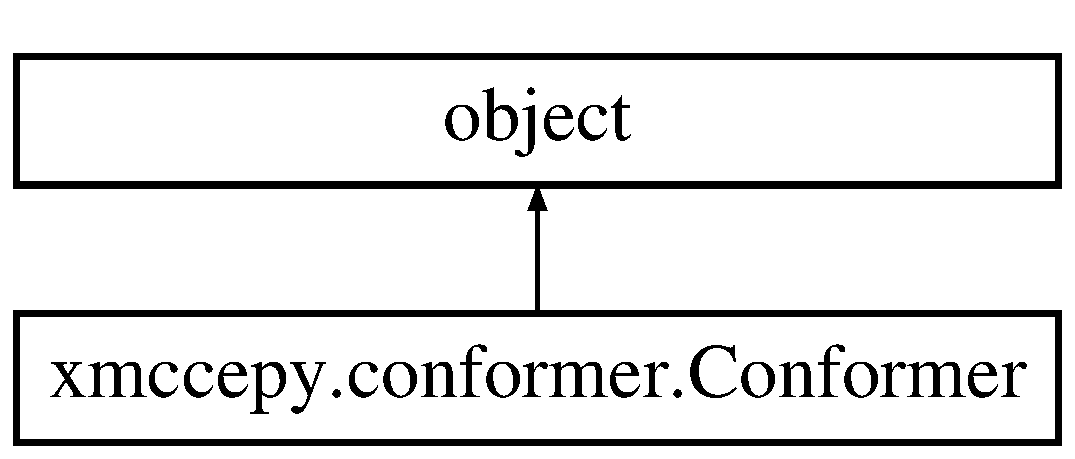
\includegraphics[height=2.000000cm]{classxmccepy_1_1conformer_1_1_conformer}
\end{center}
\end{figure}
\subsection*{Public Member Functions}
\begin{DoxyCompactItemize}
\item 
def \hyperlink{classxmccepy_1_1conformer_1_1_conformer_ace05398b4ffadf035bc7250d7da98c31}{\-\_\-\-\_\-init\-\_\-\-\_\-}
\begin{DoxyCompactList}\small\item\em Constructor. \end{DoxyCompactList}\end{DoxyCompactItemize}
\subsection*{Public Attributes}
\begin{DoxyCompactItemize}
\item 
\hyperlink{classxmccepy_1_1conformer_1_1_conformer_a717881e47510ed18cda5d11489122c5a}{conf\-Name}
\end{DoxyCompactItemize}


\subsection{Detailed Description}
Created on Apr 1, 2014. 

\begin{DoxyAuthor}{Author}
\-: xzhu \begin{DoxyVerb}Conformer class.\end{DoxyVerb}
 
\end{DoxyAuthor}


\subsection{Constructor \& Destructor Documentation}
\hypertarget{classxmccepy_1_1conformer_1_1_conformer_ace05398b4ffadf035bc7250d7da98c31}{\index{xmccepy\-::conformer\-::\-Conformer@{xmccepy\-::conformer\-::\-Conformer}!\-\_\-\-\_\-init\-\_\-\-\_\-@{\-\_\-\-\_\-init\-\_\-\-\_\-}}
\index{\-\_\-\-\_\-init\-\_\-\-\_\-@{\-\_\-\-\_\-init\-\_\-\-\_\-}!xmccepy::conformer::Conformer@{xmccepy\-::conformer\-::\-Conformer}}
\subsubsection[{\-\_\-\-\_\-init\-\_\-\-\_\-}]{\setlength{\rightskip}{0pt plus 5cm}def xmccepy.\-conformer.\-Conformer.\-\_\-\-\_\-init\-\_\-\-\_\- (
\begin{DoxyParamCaption}
\item[{}]{self}
\end{DoxyParamCaption}
)}}\label{classxmccepy_1_1conformer_1_1_conformer_ace05398b4ffadf035bc7250d7da98c31}


Constructor. 



\subsection{Member Data Documentation}
\hypertarget{classxmccepy_1_1conformer_1_1_conformer_a717881e47510ed18cda5d11489122c5a}{\index{xmccepy\-::conformer\-::\-Conformer@{xmccepy\-::conformer\-::\-Conformer}!conf\-Name@{conf\-Name}}
\index{conf\-Name@{conf\-Name}!xmccepy::conformer::Conformer@{xmccepy\-::conformer\-::\-Conformer}}
\subsubsection[{conf\-Name}]{\setlength{\rightskip}{0pt plus 5cm}xmccepy.\-conformer.\-Conformer.\-conf\-Name}}\label{classxmccepy_1_1conformer_1_1_conformer_a717881e47510ed18cda5d11489122c5a}


The documentation for this class was generated from the following file\-:\begin{DoxyCompactItemize}
\item 
src/xmccepy/\hyperlink{conformer_8py}{conformer.\-py}\end{DoxyCompactItemize}

\hypertarget{classxmccepy_1_1corr_1_1_corr}{\section{xmccepy.\-corr.\-Corr Class Reference}
\label{classxmccepy_1_1corr_1_1_corr}\index{xmccepy.\-corr.\-Corr@{xmccepy.\-corr.\-Corr}}
}


A class for the coordinate of a position.  


Inheritance diagram for xmccepy.\-corr.\-Corr\-:\begin{figure}[H]
\begin{center}
\leavevmode
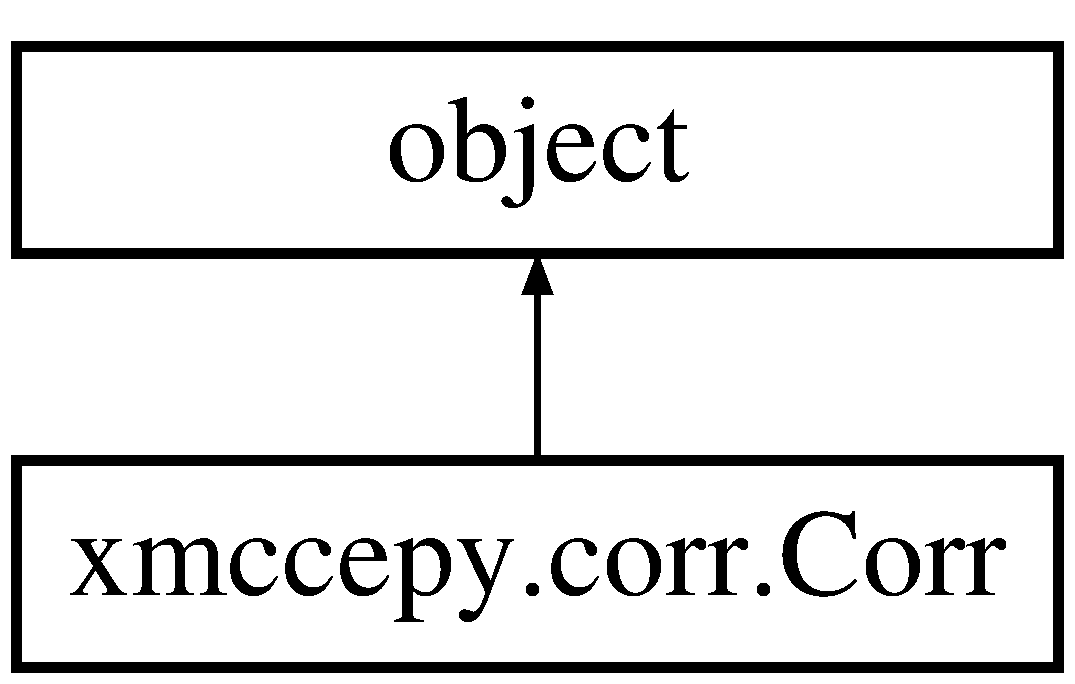
\includegraphics[height=2.000000cm]{classxmccepy_1_1corr_1_1_corr}
\end{center}
\end{figure}
\subsection*{Public Member Functions}
\begin{DoxyCompactItemize}
\item 
def \hyperlink{classxmccepy_1_1corr_1_1_corr_ab9af2823d754b0458bd814cc0ffa6d55}{\-\_\-\-\_\-init\-\_\-\-\_\-}
\begin{DoxyCompactList}\small\item\em Constructor. \end{DoxyCompactList}\item 
def \hyperlink{classxmccepy_1_1corr_1_1_corr_afdc411e79f72e2728c9eb5db1fba693f}{set}
\begin{DoxyCompactList}\small\item\em Set the x, y, z values of a coordinate. \end{DoxyCompactList}\end{DoxyCompactItemize}
\subsection*{Public Attributes}
\begin{DoxyCompactItemize}
\item 
\hyperlink{classxmccepy_1_1corr_1_1_corr_af92bf6894f8092d64bebdd641fba09f7}{x}
\item 
\hyperlink{classxmccepy_1_1corr_1_1_corr_a6a9298c2b8c4747dbd514dcde6b4e98d}{y}
\item 
\hyperlink{classxmccepy_1_1corr_1_1_corr_af4b31d22cd5524607542063be5b86a82}{z}
\end{DoxyCompactItemize}


\subsection{Detailed Description}
A class for the coordinate of a position. 

Created on Apr 1, 2014

\begin{DoxyAuthor}{Author}
\-: xzhu \begin{DoxyVerb}Corrdinate class.\end{DoxyVerb}
 
\end{DoxyAuthor}


\subsection{Constructor \& Destructor Documentation}
\hypertarget{classxmccepy_1_1corr_1_1_corr_ab9af2823d754b0458bd814cc0ffa6d55}{\index{xmccepy\-::corr\-::\-Corr@{xmccepy\-::corr\-::\-Corr}!\-\_\-\-\_\-init\-\_\-\-\_\-@{\-\_\-\-\_\-init\-\_\-\-\_\-}}
\index{\-\_\-\-\_\-init\-\_\-\-\_\-@{\-\_\-\-\_\-init\-\_\-\-\_\-}!xmccepy::corr::Corr@{xmccepy\-::corr\-::\-Corr}}
\subsubsection[{\-\_\-\-\_\-init\-\_\-\-\_\-}]{\setlength{\rightskip}{0pt plus 5cm}def xmccepy.\-corr.\-Corr.\-\_\-\-\_\-init\-\_\-\-\_\- (
\begin{DoxyParamCaption}
\item[{}]{self, }
\item[{}]{x = {\ttfamily 0.0}, }
\item[{}]{y = {\ttfamily 0.0}, }
\item[{}]{z = {\ttfamily 0.0}}
\end{DoxyParamCaption}
)}}\label{classxmccepy_1_1corr_1_1_corr_ab9af2823d754b0458bd814cc0ffa6d55}


Constructor. 



\subsection{Member Function Documentation}
\hypertarget{classxmccepy_1_1corr_1_1_corr_afdc411e79f72e2728c9eb5db1fba693f}{\index{xmccepy\-::corr\-::\-Corr@{xmccepy\-::corr\-::\-Corr}!set@{set}}
\index{set@{set}!xmccepy::corr::Corr@{xmccepy\-::corr\-::\-Corr}}
\subsubsection[{set}]{\setlength{\rightskip}{0pt plus 5cm}def xmccepy.\-corr.\-Corr.\-set (
\begin{DoxyParamCaption}
\item[{}]{self, }
\item[{}]{x = {\ttfamily 0.0}, }
\item[{}]{y = {\ttfamily 0.0}, }
\item[{}]{z = {\ttfamily 0.0}}
\end{DoxyParamCaption}
)}}\label{classxmccepy_1_1corr_1_1_corr_afdc411e79f72e2728c9eb5db1fba693f}


Set the x, y, z values of a coordinate. 



\subsection{Member Data Documentation}
\hypertarget{classxmccepy_1_1corr_1_1_corr_af92bf6894f8092d64bebdd641fba09f7}{\index{xmccepy\-::corr\-::\-Corr@{xmccepy\-::corr\-::\-Corr}!x@{x}}
\index{x@{x}!xmccepy::corr::Corr@{xmccepy\-::corr\-::\-Corr}}
\subsubsection[{x}]{\setlength{\rightskip}{0pt plus 5cm}xmccepy.\-corr.\-Corr.\-x}}\label{classxmccepy_1_1corr_1_1_corr_af92bf6894f8092d64bebdd641fba09f7}
\hypertarget{classxmccepy_1_1corr_1_1_corr_a6a9298c2b8c4747dbd514dcde6b4e98d}{\index{xmccepy\-::corr\-::\-Corr@{xmccepy\-::corr\-::\-Corr}!y@{y}}
\index{y@{y}!xmccepy::corr::Corr@{xmccepy\-::corr\-::\-Corr}}
\subsubsection[{y}]{\setlength{\rightskip}{0pt plus 5cm}xmccepy.\-corr.\-Corr.\-y}}\label{classxmccepy_1_1corr_1_1_corr_a6a9298c2b8c4747dbd514dcde6b4e98d}
\hypertarget{classxmccepy_1_1corr_1_1_corr_af4b31d22cd5524607542063be5b86a82}{\index{xmccepy\-::corr\-::\-Corr@{xmccepy\-::corr\-::\-Corr}!z@{z}}
\index{z@{z}!xmccepy::corr::Corr@{xmccepy\-::corr\-::\-Corr}}
\subsubsection[{z}]{\setlength{\rightskip}{0pt plus 5cm}xmccepy.\-corr.\-Corr.\-z}}\label{classxmccepy_1_1corr_1_1_corr_af4b31d22cd5524607542063be5b86a82}


The documentation for this class was generated from the following file\-:\begin{DoxyCompactItemize}
\item 
src/xmccepy/\hyperlink{corr_8py}{corr.\-py}\end{DoxyCompactItemize}

\hypertarget{classget__path__barrier_1_1_hb_path}{\section{get\-\_\-path\-\_\-barrier.\-Hb\-Path Class Reference}
\label{classget__path__barrier_1_1_hb_path}\index{get\-\_\-path\-\_\-barrier.\-Hb\-Path@{get\-\_\-path\-\_\-barrier.\-Hb\-Path}}
}
Inheritance diagram for get\-\_\-path\-\_\-barrier.\-Hb\-Path\-:\begin{figure}[H]
\begin{center}
\leavevmode
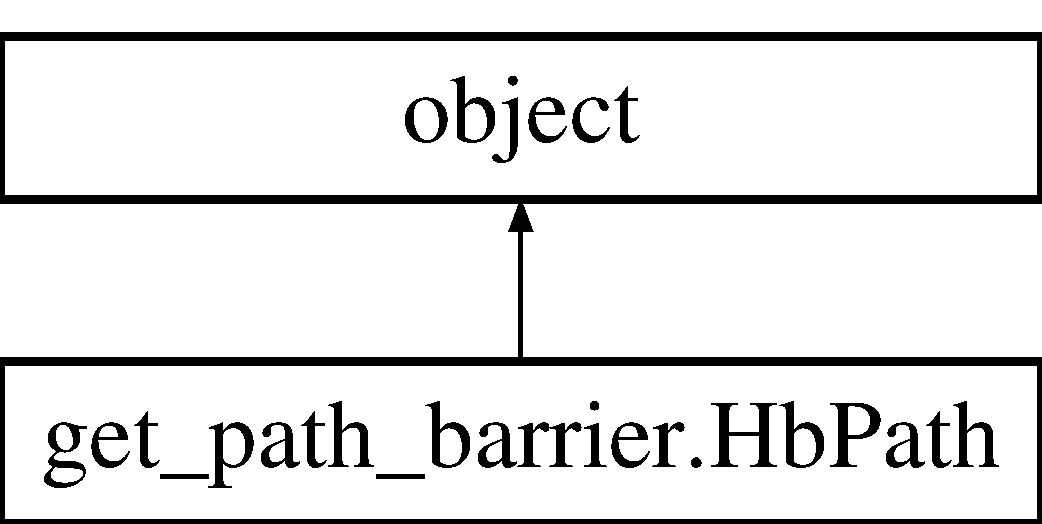
\includegraphics[height=2.000000cm]{classget__path__barrier_1_1_hb_path}
\end{center}
\end{figure}
\subsection*{Public Member Functions}
\begin{DoxyCompactItemize}
\item 
def \hyperlink{classget__path__barrier_1_1_hb_path_ac8526be6c34f93d3991d772e51ac2dd0}{\-\_\-\-\_\-init\-\_\-\-\_\-}
\item 
def \hyperlink{classget__path__barrier_1_1_hb_path_aba025f763752636443417573fc82e941}{load\-Path\-Info}
\begin{DoxyCompactList}\small\item\em Get the key residues in the pathway, and their possible protonation states, and the initial state. \end{DoxyCompactList}\item 
def \hyperlink{classget__path__barrier_1_1_hb_path_a7b689f661b263b4a027559f306b44567}{get\-All\-Hop\-Sequences}
\end{DoxyCompactItemize}
\subsection*{Public Attributes}
\begin{DoxyCompactItemize}
\item 
\hyperlink{classget__path__barrier_1_1_hb_path_af574f30a4a9297c5b798a9f5ab93429c}{key\-Residues}
\item 
\hyperlink{classget__path__barrier_1_1_hb_path_aa3cc8420eaf75f40689de3c1c4ef9143}{possible\-Protonations}
\item 
\hyperlink{classget__path__barrier_1_1_hb_path_acb500e7ef9452b85d3a037ae96b952d3}{initial\-State}
\item 
\hyperlink{classget__path__barrier_1_1_hb_path_abde19f996710977a200bbd380327d992}{n\-Residues}
\item 
\hyperlink{classget__path__barrier_1_1_hb_path_a838cc727a1853ae9dbcda45158c4ff1d}{hop\-Sequences}
\item 
\hyperlink{classget__path__barrier_1_1_hb_path_a232b46f1966ab71a5c5ffef1c476ac8f}{protonation\-States}
\end{DoxyCompactItemize}


\subsection{Constructor \& Destructor Documentation}
\hypertarget{classget__path__barrier_1_1_hb_path_ac8526be6c34f93d3991d772e51ac2dd0}{\index{get\-\_\-path\-\_\-barrier\-::\-Hb\-Path@{get\-\_\-path\-\_\-barrier\-::\-Hb\-Path}!\-\_\-\-\_\-init\-\_\-\-\_\-@{\-\_\-\-\_\-init\-\_\-\-\_\-}}
\index{\-\_\-\-\_\-init\-\_\-\-\_\-@{\-\_\-\-\_\-init\-\_\-\-\_\-}!get_path_barrier::HbPath@{get\-\_\-path\-\_\-barrier\-::\-Hb\-Path}}
\subsubsection[{\-\_\-\-\_\-init\-\_\-\-\_\-}]{\setlength{\rightskip}{0pt plus 5cm}def get\-\_\-path\-\_\-barrier.\-Hb\-Path.\-\_\-\-\_\-init\-\_\-\-\_\- (
\begin{DoxyParamCaption}
\item[{}]{self}
\end{DoxyParamCaption}
)}}\label{classget__path__barrier_1_1_hb_path_ac8526be6c34f93d3991d772e51ac2dd0}


\subsection{Member Function Documentation}
\hypertarget{classget__path__barrier_1_1_hb_path_a7b689f661b263b4a027559f306b44567}{\index{get\-\_\-path\-\_\-barrier\-::\-Hb\-Path@{get\-\_\-path\-\_\-barrier\-::\-Hb\-Path}!get\-All\-Hop\-Sequences@{get\-All\-Hop\-Sequences}}
\index{get\-All\-Hop\-Sequences@{get\-All\-Hop\-Sequences}!get_path_barrier::HbPath@{get\-\_\-path\-\_\-barrier\-::\-Hb\-Path}}
\subsubsection[{get\-All\-Hop\-Sequences}]{\setlength{\rightskip}{0pt plus 5cm}def get\-\_\-path\-\_\-barrier.\-Hb\-Path.\-get\-All\-Hop\-Sequences (
\begin{DoxyParamCaption}
\item[{}]{self}
\end{DoxyParamCaption}
)}}\label{classget__path__barrier_1_1_hb_path_a7b689f661b263b4a027559f306b44567}
\hypertarget{classget__path__barrier_1_1_hb_path_aba025f763752636443417573fc82e941}{\index{get\-\_\-path\-\_\-barrier\-::\-Hb\-Path@{get\-\_\-path\-\_\-barrier\-::\-Hb\-Path}!load\-Path\-Info@{load\-Path\-Info}}
\index{load\-Path\-Info@{load\-Path\-Info}!get_path_barrier::HbPath@{get\-\_\-path\-\_\-barrier\-::\-Hb\-Path}}
\subsubsection[{load\-Path\-Info}]{\setlength{\rightskip}{0pt plus 5cm}def get\-\_\-path\-\_\-barrier.\-Hb\-Path.\-load\-Path\-Info (
\begin{DoxyParamCaption}
\item[{}]{self, }
\item[{}]{f\-Name = {\ttfamily {\bf P\-A\-T\-H\-\_\-\-I\-N\-F\-O\-\_\-\-F\-I\-L\-E}}}
\end{DoxyParamCaption}
)}}\label{classget__path__barrier_1_1_hb_path_aba025f763752636443417573fc82e941}


Get the key residues in the pathway, and their possible protonation states, and the initial state. 

Return an object of class Path\-Config containing this information. \begin{DoxyVerb}    The file format should be like this:
    ASPA0085  -1  0
    HOHA0402  -1  0  1
    HOHA0406  -1  0  1
    ARGA0082   0  1
    HOHA0403  -1  0  1
    GLUA0194  -1  0
     0 0 0 1 0 -1

     The last line is the initial state.
     The other lines give the name of the residues, following all their possible protonation states\end{DoxyVerb}
 

\subsection{Member Data Documentation}
\hypertarget{classget__path__barrier_1_1_hb_path_a838cc727a1853ae9dbcda45158c4ff1d}{\index{get\-\_\-path\-\_\-barrier\-::\-Hb\-Path@{get\-\_\-path\-\_\-barrier\-::\-Hb\-Path}!hop\-Sequences@{hop\-Sequences}}
\index{hop\-Sequences@{hop\-Sequences}!get_path_barrier::HbPath@{get\-\_\-path\-\_\-barrier\-::\-Hb\-Path}}
\subsubsection[{hop\-Sequences}]{\setlength{\rightskip}{0pt plus 5cm}get\-\_\-path\-\_\-barrier.\-Hb\-Path.\-hop\-Sequences}}\label{classget__path__barrier_1_1_hb_path_a838cc727a1853ae9dbcda45158c4ff1d}
\hypertarget{classget__path__barrier_1_1_hb_path_acb500e7ef9452b85d3a037ae96b952d3}{\index{get\-\_\-path\-\_\-barrier\-::\-Hb\-Path@{get\-\_\-path\-\_\-barrier\-::\-Hb\-Path}!initial\-State@{initial\-State}}
\index{initial\-State@{initial\-State}!get_path_barrier::HbPath@{get\-\_\-path\-\_\-barrier\-::\-Hb\-Path}}
\subsubsection[{initial\-State}]{\setlength{\rightskip}{0pt plus 5cm}get\-\_\-path\-\_\-barrier.\-Hb\-Path.\-initial\-State}}\label{classget__path__barrier_1_1_hb_path_acb500e7ef9452b85d3a037ae96b952d3}
\hypertarget{classget__path__barrier_1_1_hb_path_af574f30a4a9297c5b798a9f5ab93429c}{\index{get\-\_\-path\-\_\-barrier\-::\-Hb\-Path@{get\-\_\-path\-\_\-barrier\-::\-Hb\-Path}!key\-Residues@{key\-Residues}}
\index{key\-Residues@{key\-Residues}!get_path_barrier::HbPath@{get\-\_\-path\-\_\-barrier\-::\-Hb\-Path}}
\subsubsection[{key\-Residues}]{\setlength{\rightskip}{0pt plus 5cm}get\-\_\-path\-\_\-barrier.\-Hb\-Path.\-key\-Residues}}\label{classget__path__barrier_1_1_hb_path_af574f30a4a9297c5b798a9f5ab93429c}
\hypertarget{classget__path__barrier_1_1_hb_path_abde19f996710977a200bbd380327d992}{\index{get\-\_\-path\-\_\-barrier\-::\-Hb\-Path@{get\-\_\-path\-\_\-barrier\-::\-Hb\-Path}!n\-Residues@{n\-Residues}}
\index{n\-Residues@{n\-Residues}!get_path_barrier::HbPath@{get\-\_\-path\-\_\-barrier\-::\-Hb\-Path}}
\subsubsection[{n\-Residues}]{\setlength{\rightskip}{0pt plus 5cm}get\-\_\-path\-\_\-barrier.\-Hb\-Path.\-n\-Residues}}\label{classget__path__barrier_1_1_hb_path_abde19f996710977a200bbd380327d992}
\hypertarget{classget__path__barrier_1_1_hb_path_aa3cc8420eaf75f40689de3c1c4ef9143}{\index{get\-\_\-path\-\_\-barrier\-::\-Hb\-Path@{get\-\_\-path\-\_\-barrier\-::\-Hb\-Path}!possible\-Protonations@{possible\-Protonations}}
\index{possible\-Protonations@{possible\-Protonations}!get_path_barrier::HbPath@{get\-\_\-path\-\_\-barrier\-::\-Hb\-Path}}
\subsubsection[{possible\-Protonations}]{\setlength{\rightskip}{0pt plus 5cm}get\-\_\-path\-\_\-barrier.\-Hb\-Path.\-possible\-Protonations}}\label{classget__path__barrier_1_1_hb_path_aa3cc8420eaf75f40689de3c1c4ef9143}
\hypertarget{classget__path__barrier_1_1_hb_path_a232b46f1966ab71a5c5ffef1c476ac8f}{\index{get\-\_\-path\-\_\-barrier\-::\-Hb\-Path@{get\-\_\-path\-\_\-barrier\-::\-Hb\-Path}!protonation\-States@{protonation\-States}}
\index{protonation\-States@{protonation\-States}!get_path_barrier::HbPath@{get\-\_\-path\-\_\-barrier\-::\-Hb\-Path}}
\subsubsection[{protonation\-States}]{\setlength{\rightskip}{0pt plus 5cm}get\-\_\-path\-\_\-barrier.\-Hb\-Path.\-protonation\-States}}\label{classget__path__barrier_1_1_hb_path_a232b46f1966ab71a5c5ffef1c476ac8f}


The documentation for this class was generated from the following file\-:\begin{DoxyCompactItemize}
\item 
src/path\-\_\-analysis/\hyperlink{get__path__barrier_8py}{get\-\_\-path\-\_\-barrier.\-py}\end{DoxyCompactItemize}

\hypertarget{classget__path__barrier_1_1_hop_sequence}{\section{get\-\_\-path\-\_\-barrier.\-Hop\-Sequence Class Reference}
\label{classget__path__barrier_1_1_hop_sequence}\index{get\-\_\-path\-\_\-barrier.\-Hop\-Sequence@{get\-\_\-path\-\_\-barrier.\-Hop\-Sequence}}
}
Inheritance diagram for get\-\_\-path\-\_\-barrier.\-Hop\-Sequence\-:\begin{figure}[H]
\begin{center}
\leavevmode
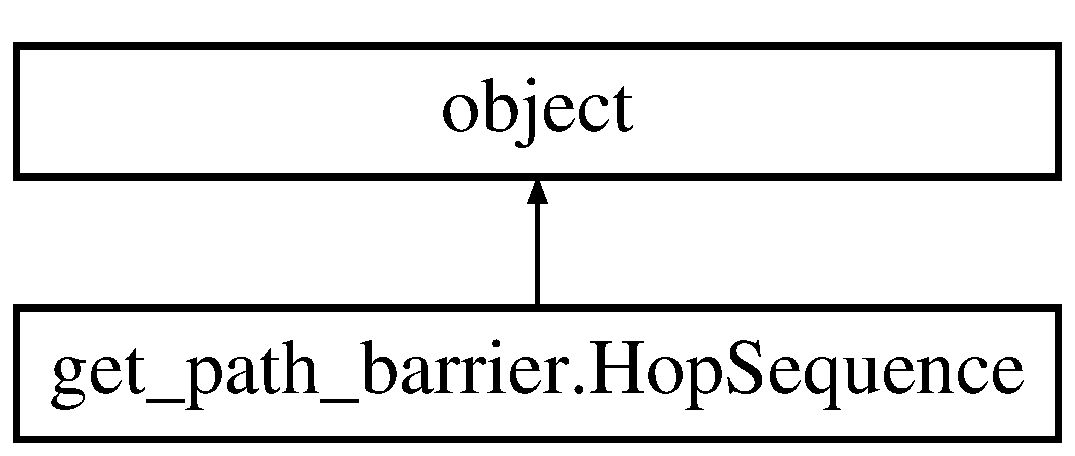
\includegraphics[height=2.000000cm]{classget__path__barrier_1_1_hop_sequence}
\end{center}
\end{figure}
\subsection*{Public Member Functions}
\begin{DoxyCompactItemize}
\item 
def \hyperlink{classget__path__barrier_1_1_hop_sequence_a3e4932d6b92f4c4cdd2c75af9139471d}{\-\_\-\-\_\-init\-\_\-\-\_\-}
\item 
def \hyperlink{classget__path__barrier_1_1_hop_sequence_ad1899d97aecd2215fd82075ce23f606a}{next\-Hop}
\item 
def \hyperlink{classget__path__barrier_1_1_hop_sequence_a50093adf1d30dca2b491fb549e3e5225}{get\-E\-Barrier}
\end{DoxyCompactItemize}
\subsection*{Public Attributes}
\begin{DoxyCompactItemize}
\item 
\hyperlink{classget__path__barrier_1_1_hop_sequence_a579cbd71947f980116542947f6fc3bb3}{hop\-History}
\item 
\hyperlink{classget__path__barrier_1_1_hop_sequence_a0bcfd627eb7a3a1adbcea611d1e4b6a6}{energy\-Barrier}
\item 
\hyperlink{classget__path__barrier_1_1_hop_sequence_aa539256b485b15e0bfb1388e832c4060}{intermediates}
\end{DoxyCompactItemize}
\subsection*{Static Public Attributes}
\begin{DoxyCompactItemize}
\item 
list \hyperlink{classget__path__barrier_1_1_hop_sequence_a1ddfff32b9b3d13841eaf9fcaceba041}{possible\-Protonations} = \mbox{[}$\,$\mbox{]}
\end{DoxyCompactItemize}


\subsection{Constructor \& Destructor Documentation}
\hypertarget{classget__path__barrier_1_1_hop_sequence_a3e4932d6b92f4c4cdd2c75af9139471d}{\index{get\-\_\-path\-\_\-barrier\-::\-Hop\-Sequence@{get\-\_\-path\-\_\-barrier\-::\-Hop\-Sequence}!\-\_\-\-\_\-init\-\_\-\-\_\-@{\-\_\-\-\_\-init\-\_\-\-\_\-}}
\index{\-\_\-\-\_\-init\-\_\-\-\_\-@{\-\_\-\-\_\-init\-\_\-\-\_\-}!get_path_barrier::HopSequence@{get\-\_\-path\-\_\-barrier\-::\-Hop\-Sequence}}
\subsubsection[{\-\_\-\-\_\-init\-\_\-\-\_\-}]{\setlength{\rightskip}{0pt plus 5cm}def get\-\_\-path\-\_\-barrier.\-Hop\-Sequence.\-\_\-\-\_\-init\-\_\-\-\_\- (
\begin{DoxyParamCaption}
\item[{}]{self, }
\item[{}]{initial\-State = {\ttfamily None}}
\end{DoxyParamCaption}
)}}\label{classget__path__barrier_1_1_hop_sequence_a3e4932d6b92f4c4cdd2c75af9139471d}


\subsection{Member Function Documentation}
\hypertarget{classget__path__barrier_1_1_hop_sequence_a50093adf1d30dca2b491fb549e3e5225}{\index{get\-\_\-path\-\_\-barrier\-::\-Hop\-Sequence@{get\-\_\-path\-\_\-barrier\-::\-Hop\-Sequence}!get\-E\-Barrier@{get\-E\-Barrier}}
\index{get\-E\-Barrier@{get\-E\-Barrier}!get_path_barrier::HopSequence@{get\-\_\-path\-\_\-barrier\-::\-Hop\-Sequence}}
\subsubsection[{get\-E\-Barrier}]{\setlength{\rightskip}{0pt plus 5cm}def get\-\_\-path\-\_\-barrier.\-Hop\-Sequence.\-get\-E\-Barrier (
\begin{DoxyParamCaption}
\item[{}]{self}
\end{DoxyParamCaption}
)}}\label{classget__path__barrier_1_1_hop_sequence_a50093adf1d30dca2b491fb549e3e5225}
\hypertarget{classget__path__barrier_1_1_hop_sequence_ad1899d97aecd2215fd82075ce23f606a}{\index{get\-\_\-path\-\_\-barrier\-::\-Hop\-Sequence@{get\-\_\-path\-\_\-barrier\-::\-Hop\-Sequence}!next\-Hop@{next\-Hop}}
\index{next\-Hop@{next\-Hop}!get_path_barrier::HopSequence@{get\-\_\-path\-\_\-barrier\-::\-Hop\-Sequence}}
\subsubsection[{next\-Hop}]{\setlength{\rightskip}{0pt plus 5cm}def get\-\_\-path\-\_\-barrier.\-Hop\-Sequence.\-next\-Hop (
\begin{DoxyParamCaption}
\item[{}]{self}
\end{DoxyParamCaption}
)}}\label{classget__path__barrier_1_1_hop_sequence_ad1899d97aecd2215fd82075ce23f606a}


\subsection{Member Data Documentation}
\hypertarget{classget__path__barrier_1_1_hop_sequence_a0bcfd627eb7a3a1adbcea611d1e4b6a6}{\index{get\-\_\-path\-\_\-barrier\-::\-Hop\-Sequence@{get\-\_\-path\-\_\-barrier\-::\-Hop\-Sequence}!energy\-Barrier@{energy\-Barrier}}
\index{energy\-Barrier@{energy\-Barrier}!get_path_barrier::HopSequence@{get\-\_\-path\-\_\-barrier\-::\-Hop\-Sequence}}
\subsubsection[{energy\-Barrier}]{\setlength{\rightskip}{0pt plus 5cm}get\-\_\-path\-\_\-barrier.\-Hop\-Sequence.\-energy\-Barrier}}\label{classget__path__barrier_1_1_hop_sequence_a0bcfd627eb7a3a1adbcea611d1e4b6a6}
\hypertarget{classget__path__barrier_1_1_hop_sequence_a579cbd71947f980116542947f6fc3bb3}{\index{get\-\_\-path\-\_\-barrier\-::\-Hop\-Sequence@{get\-\_\-path\-\_\-barrier\-::\-Hop\-Sequence}!hop\-History@{hop\-History}}
\index{hop\-History@{hop\-History}!get_path_barrier::HopSequence@{get\-\_\-path\-\_\-barrier\-::\-Hop\-Sequence}}
\subsubsection[{hop\-History}]{\setlength{\rightskip}{0pt plus 5cm}get\-\_\-path\-\_\-barrier.\-Hop\-Sequence.\-hop\-History}}\label{classget__path__barrier_1_1_hop_sequence_a579cbd71947f980116542947f6fc3bb3}
\hypertarget{classget__path__barrier_1_1_hop_sequence_aa539256b485b15e0bfb1388e832c4060}{\index{get\-\_\-path\-\_\-barrier\-::\-Hop\-Sequence@{get\-\_\-path\-\_\-barrier\-::\-Hop\-Sequence}!intermediates@{intermediates}}
\index{intermediates@{intermediates}!get_path_barrier::HopSequence@{get\-\_\-path\-\_\-barrier\-::\-Hop\-Sequence}}
\subsubsection[{intermediates}]{\setlength{\rightskip}{0pt plus 5cm}get\-\_\-path\-\_\-barrier.\-Hop\-Sequence.\-intermediates}}\label{classget__path__barrier_1_1_hop_sequence_aa539256b485b15e0bfb1388e832c4060}
\hypertarget{classget__path__barrier_1_1_hop_sequence_a1ddfff32b9b3d13841eaf9fcaceba041}{\index{get\-\_\-path\-\_\-barrier\-::\-Hop\-Sequence@{get\-\_\-path\-\_\-barrier\-::\-Hop\-Sequence}!possible\-Protonations@{possible\-Protonations}}
\index{possible\-Protonations@{possible\-Protonations}!get_path_barrier::HopSequence@{get\-\_\-path\-\_\-barrier\-::\-Hop\-Sequence}}
\subsubsection[{possible\-Protonations}]{\setlength{\rightskip}{0pt plus 5cm}list get\-\_\-path\-\_\-barrier.\-Hop\-Sequence.\-possible\-Protonations = \mbox{[}$\,$\mbox{]}\hspace{0.3cm}{\ttfamily [static]}}}\label{classget__path__barrier_1_1_hop_sequence_a1ddfff32b9b3d13841eaf9fcaceba041}


The documentation for this class was generated from the following file\-:\begin{DoxyCompactItemize}
\item 
src/path\-\_\-analysis/\hyperlink{get__path__barrier_8py}{get\-\_\-path\-\_\-barrier.\-py}\end{DoxyCompactItemize}

\hypertarget{classxmccepy_1_1mp_1_1_p_r_o_t_e_i_n}{\section{xmccepy.\-mp.\-P\-R\-O\-T\-E\-I\-N Class Reference}
\label{classxmccepy_1_1mp_1_1_p_r_o_t_e_i_n}\index{xmccepy.\-mp.\-P\-R\-O\-T\-E\-I\-N@{xmccepy.\-mp.\-P\-R\-O\-T\-E\-I\-N}}
}
\subsection*{Public Member Functions}
\begin{DoxyCompactItemize}
\item 
def \hyperlink{classxmccepy_1_1mp_1_1_p_r_o_t_e_i_n_a7e26d4d1cfd60c6a5193c141971dbc05}{\-\_\-\-\_\-init\-\_\-\-\_\-}
\item 
def \hyperlink{classxmccepy_1_1mp_1_1_p_r_o_t_e_i_n_a64b0e15c69b786fa85740bd7416b6d42}{read\-P\-D\-B}
\item 
def \hyperlink{classxmccepy_1_1mp_1_1_p_r_o_t_e_i_n_ae9f72597d99182414e3afe867d0c0997}{write\-P\-D\-B}
\end{DoxyCompactItemize}
\subsection*{Public Attributes}
\begin{DoxyCompactItemize}
\item 
\hyperlink{classxmccepy_1_1mp_1_1_p_r_o_t_e_i_n_ae97e1a5a6da630ad7de620df7ce17439}{ress}
\end{DoxyCompactItemize}


\subsection{Constructor \& Destructor Documentation}
\hypertarget{classxmccepy_1_1mp_1_1_p_r_o_t_e_i_n_a7e26d4d1cfd60c6a5193c141971dbc05}{\index{xmccepy\-::mp\-::\-P\-R\-O\-T\-E\-I\-N@{xmccepy\-::mp\-::\-P\-R\-O\-T\-E\-I\-N}!\-\_\-\-\_\-init\-\_\-\-\_\-@{\-\_\-\-\_\-init\-\_\-\-\_\-}}
\index{\-\_\-\-\_\-init\-\_\-\-\_\-@{\-\_\-\-\_\-init\-\_\-\-\_\-}!xmccepy::mp::PROTEIN@{xmccepy\-::mp\-::\-P\-R\-O\-T\-E\-I\-N}}
\subsubsection[{\-\_\-\-\_\-init\-\_\-\-\_\-}]{\setlength{\rightskip}{0pt plus 5cm}def xmccepy.\-mp.\-P\-R\-O\-T\-E\-I\-N.\-\_\-\-\_\-init\-\_\-\-\_\- (
\begin{DoxyParamCaption}
\item[{}]{self}
\end{DoxyParamCaption}
)}}\label{classxmccepy_1_1mp_1_1_p_r_o_t_e_i_n_a7e26d4d1cfd60c6a5193c141971dbc05}


\subsection{Member Function Documentation}
\hypertarget{classxmccepy_1_1mp_1_1_p_r_o_t_e_i_n_a64b0e15c69b786fa85740bd7416b6d42}{\index{xmccepy\-::mp\-::\-P\-R\-O\-T\-E\-I\-N@{xmccepy\-::mp\-::\-P\-R\-O\-T\-E\-I\-N}!read\-P\-D\-B@{read\-P\-D\-B}}
\index{read\-P\-D\-B@{read\-P\-D\-B}!xmccepy::mp::PROTEIN@{xmccepy\-::mp\-::\-P\-R\-O\-T\-E\-I\-N}}
\subsubsection[{read\-P\-D\-B}]{\setlength{\rightskip}{0pt plus 5cm}def xmccepy.\-mp.\-P\-R\-O\-T\-E\-I\-N.\-read\-P\-D\-B (
\begin{DoxyParamCaption}
\item[{}]{self, }
\item[{}]{fname}
\end{DoxyParamCaption}
)}}\label{classxmccepy_1_1mp_1_1_p_r_o_t_e_i_n_a64b0e15c69b786fa85740bd7416b6d42}
\hypertarget{classxmccepy_1_1mp_1_1_p_r_o_t_e_i_n_ae9f72597d99182414e3afe867d0c0997}{\index{xmccepy\-::mp\-::\-P\-R\-O\-T\-E\-I\-N@{xmccepy\-::mp\-::\-P\-R\-O\-T\-E\-I\-N}!write\-P\-D\-B@{write\-P\-D\-B}}
\index{write\-P\-D\-B@{write\-P\-D\-B}!xmccepy::mp::PROTEIN@{xmccepy\-::mp\-::\-P\-R\-O\-T\-E\-I\-N}}
\subsubsection[{write\-P\-D\-B}]{\setlength{\rightskip}{0pt plus 5cm}def xmccepy.\-mp.\-P\-R\-O\-T\-E\-I\-N.\-write\-P\-D\-B (
\begin{DoxyParamCaption}
\item[{}]{self}
\end{DoxyParamCaption}
)}}\label{classxmccepy_1_1mp_1_1_p_r_o_t_e_i_n_ae9f72597d99182414e3afe867d0c0997}


\subsection{Member Data Documentation}
\hypertarget{classxmccepy_1_1mp_1_1_p_r_o_t_e_i_n_ae97e1a5a6da630ad7de620df7ce17439}{\index{xmccepy\-::mp\-::\-P\-R\-O\-T\-E\-I\-N@{xmccepy\-::mp\-::\-P\-R\-O\-T\-E\-I\-N}!ress@{ress}}
\index{ress@{ress}!xmccepy::mp::PROTEIN@{xmccepy\-::mp\-::\-P\-R\-O\-T\-E\-I\-N}}
\subsubsection[{ress}]{\setlength{\rightskip}{0pt plus 5cm}xmccepy.\-mp.\-P\-R\-O\-T\-E\-I\-N.\-ress}}\label{classxmccepy_1_1mp_1_1_p_r_o_t_e_i_n_ae97e1a5a6da630ad7de620df7ce17439}


The documentation for this class was generated from the following file\-:\begin{DoxyCompactItemize}
\item 
src/xmccepy/\hyperlink{mp_8py}{mp.\-py}\end{DoxyCompactItemize}

\hypertarget{classget__path__barrier_1_1_protonation_state}{\section{get\-\_\-path\-\_\-barrier.\-Protonation\-State Class Reference}
\label{classget__path__barrier_1_1_protonation_state}\index{get\-\_\-path\-\_\-barrier.\-Protonation\-State@{get\-\_\-path\-\_\-barrier.\-Protonation\-State}}
}
Inheritance diagram for get\-\_\-path\-\_\-barrier.\-Protonation\-State\-:\begin{figure}[H]
\begin{center}
\leavevmode
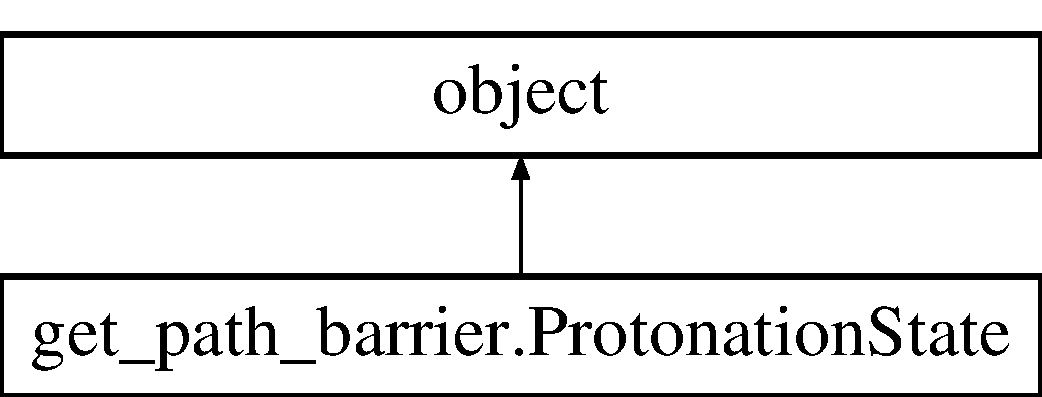
\includegraphics[height=2.000000cm]{classget__path__barrier_1_1_protonation_state}
\end{center}
\end{figure}
\subsection*{Public Member Functions}
\begin{DoxyCompactItemize}
\item 
def \hyperlink{classget__path__barrier_1_1_protonation_state_a5e56262319e3d5d2a72aa81aa0955bc9}{\-\_\-\-\_\-init\-\_\-\-\_\-}
\item 
def \hyperlink{classget__path__barrier_1_1_protonation_state_af592e055063b5b7f253725fbabe0c7ee}{\-\_\-\-\_\-repr\-\_\-\-\_\-}
\item 
def \hyperlink{classget__path__barrier_1_1_protonation_state_a37bf6b1faf41f3e5a7885153479cfc7a}{\-\_\-\-\_\-eq\-\_\-\-\_\-}
\item 
def \hyperlink{classget__path__barrier_1_1_protonation_state_ae47205464189ac09427afaafa2d490d0}{\-\_\-\-\_\-hash\-\_\-\-\_\-}
\end{DoxyCompactItemize}
\subsection*{Public Attributes}
\begin{DoxyCompactItemize}
\item 
\hyperlink{classget__path__barrier_1_1_protonation_state_ab17df337fcf1611aae2ca3d32c7d9925}{protonations}
\item 
\hyperlink{classget__path__barrier_1_1_protonation_state_a26b22fd31a45e001adadace05453862c}{energy}
\item 
\hyperlink{classget__path__barrier_1_1_protonation_state_a0887568cf1ad7ef61b03b9e9e0438186}{state\-Id}
\item 
\hyperlink{classget__path__barrier_1_1_protonation_state_afa1e7d9c2e2721bb0eaacaff5729e68f}{layer}
\end{DoxyCompactItemize}
\subsection*{Static Public Attributes}
\begin{DoxyCompactItemize}
\item 
list \hyperlink{classget__path__barrier_1_1_protonation_state_a6619f2acd36f3f2cfd1358e2912b6a97}{key\-Residues} = \mbox{[}$\,$\mbox{]}
\end{DoxyCompactItemize}


\subsection{Constructor \& Destructor Documentation}
\hypertarget{classget__path__barrier_1_1_protonation_state_a5e56262319e3d5d2a72aa81aa0955bc9}{\index{get\-\_\-path\-\_\-barrier\-::\-Protonation\-State@{get\-\_\-path\-\_\-barrier\-::\-Protonation\-State}!\-\_\-\-\_\-init\-\_\-\-\_\-@{\-\_\-\-\_\-init\-\_\-\-\_\-}}
\index{\-\_\-\-\_\-init\-\_\-\-\_\-@{\-\_\-\-\_\-init\-\_\-\-\_\-}!get_path_barrier::ProtonationState@{get\-\_\-path\-\_\-barrier\-::\-Protonation\-State}}
\subsubsection[{\-\_\-\-\_\-init\-\_\-\-\_\-}]{\setlength{\rightskip}{0pt plus 5cm}def get\-\_\-path\-\_\-barrier.\-Protonation\-State.\-\_\-\-\_\-init\-\_\-\-\_\- (
\begin{DoxyParamCaption}
\item[{}]{self}
\end{DoxyParamCaption}
)}}\label{classget__path__barrier_1_1_protonation_state_a5e56262319e3d5d2a72aa81aa0955bc9}


\subsection{Member Function Documentation}
\hypertarget{classget__path__barrier_1_1_protonation_state_a37bf6b1faf41f3e5a7885153479cfc7a}{\index{get\-\_\-path\-\_\-barrier\-::\-Protonation\-State@{get\-\_\-path\-\_\-barrier\-::\-Protonation\-State}!\-\_\-\-\_\-eq\-\_\-\-\_\-@{\-\_\-\-\_\-eq\-\_\-\-\_\-}}
\index{\-\_\-\-\_\-eq\-\_\-\-\_\-@{\-\_\-\-\_\-eq\-\_\-\-\_\-}!get_path_barrier::ProtonationState@{get\-\_\-path\-\_\-barrier\-::\-Protonation\-State}}
\subsubsection[{\-\_\-\-\_\-eq\-\_\-\-\_\-}]{\setlength{\rightskip}{0pt plus 5cm}def get\-\_\-path\-\_\-barrier.\-Protonation\-State.\-\_\-\-\_\-eq\-\_\-\-\_\- (
\begin{DoxyParamCaption}
\item[{}]{self, }
\item[{}]{other}
\end{DoxyParamCaption}
)}}\label{classget__path__barrier_1_1_protonation_state_a37bf6b1faf41f3e5a7885153479cfc7a}
\hypertarget{classget__path__barrier_1_1_protonation_state_ae47205464189ac09427afaafa2d490d0}{\index{get\-\_\-path\-\_\-barrier\-::\-Protonation\-State@{get\-\_\-path\-\_\-barrier\-::\-Protonation\-State}!\-\_\-\-\_\-hash\-\_\-\-\_\-@{\-\_\-\-\_\-hash\-\_\-\-\_\-}}
\index{\-\_\-\-\_\-hash\-\_\-\-\_\-@{\-\_\-\-\_\-hash\-\_\-\-\_\-}!get_path_barrier::ProtonationState@{get\-\_\-path\-\_\-barrier\-::\-Protonation\-State}}
\subsubsection[{\-\_\-\-\_\-hash\-\_\-\-\_\-}]{\setlength{\rightskip}{0pt plus 5cm}def get\-\_\-path\-\_\-barrier.\-Protonation\-State.\-\_\-\-\_\-hash\-\_\-\-\_\- (
\begin{DoxyParamCaption}
\item[{}]{self}
\end{DoxyParamCaption}
)}}\label{classget__path__barrier_1_1_protonation_state_ae47205464189ac09427afaafa2d490d0}
\hypertarget{classget__path__barrier_1_1_protonation_state_af592e055063b5b7f253725fbabe0c7ee}{\index{get\-\_\-path\-\_\-barrier\-::\-Protonation\-State@{get\-\_\-path\-\_\-barrier\-::\-Protonation\-State}!\-\_\-\-\_\-repr\-\_\-\-\_\-@{\-\_\-\-\_\-repr\-\_\-\-\_\-}}
\index{\-\_\-\-\_\-repr\-\_\-\-\_\-@{\-\_\-\-\_\-repr\-\_\-\-\_\-}!get_path_barrier::ProtonationState@{get\-\_\-path\-\_\-barrier\-::\-Protonation\-State}}
\subsubsection[{\-\_\-\-\_\-repr\-\_\-\-\_\-}]{\setlength{\rightskip}{0pt plus 5cm}def get\-\_\-path\-\_\-barrier.\-Protonation\-State.\-\_\-\-\_\-repr\-\_\-\-\_\- (
\begin{DoxyParamCaption}
\item[{}]{self}
\end{DoxyParamCaption}
)}}\label{classget__path__barrier_1_1_protonation_state_af592e055063b5b7f253725fbabe0c7ee}


\subsection{Member Data Documentation}
\hypertarget{classget__path__barrier_1_1_protonation_state_a26b22fd31a45e001adadace05453862c}{\index{get\-\_\-path\-\_\-barrier\-::\-Protonation\-State@{get\-\_\-path\-\_\-barrier\-::\-Protonation\-State}!energy@{energy}}
\index{energy@{energy}!get_path_barrier::ProtonationState@{get\-\_\-path\-\_\-barrier\-::\-Protonation\-State}}
\subsubsection[{energy}]{\setlength{\rightskip}{0pt plus 5cm}get\-\_\-path\-\_\-barrier.\-Protonation\-State.\-energy}}\label{classget__path__barrier_1_1_protonation_state_a26b22fd31a45e001adadace05453862c}
\hypertarget{classget__path__barrier_1_1_protonation_state_a6619f2acd36f3f2cfd1358e2912b6a97}{\index{get\-\_\-path\-\_\-barrier\-::\-Protonation\-State@{get\-\_\-path\-\_\-barrier\-::\-Protonation\-State}!key\-Residues@{key\-Residues}}
\index{key\-Residues@{key\-Residues}!get_path_barrier::ProtonationState@{get\-\_\-path\-\_\-barrier\-::\-Protonation\-State}}
\subsubsection[{key\-Residues}]{\setlength{\rightskip}{0pt plus 5cm}list get\-\_\-path\-\_\-barrier.\-Protonation\-State.\-key\-Residues = \mbox{[}$\,$\mbox{]}\hspace{0.3cm}{\ttfamily [static]}}}\label{classget__path__barrier_1_1_protonation_state_a6619f2acd36f3f2cfd1358e2912b6a97}
\hypertarget{classget__path__barrier_1_1_protonation_state_afa1e7d9c2e2721bb0eaacaff5729e68f}{\index{get\-\_\-path\-\_\-barrier\-::\-Protonation\-State@{get\-\_\-path\-\_\-barrier\-::\-Protonation\-State}!layer@{layer}}
\index{layer@{layer}!get_path_barrier::ProtonationState@{get\-\_\-path\-\_\-barrier\-::\-Protonation\-State}}
\subsubsection[{layer}]{\setlength{\rightskip}{0pt plus 5cm}get\-\_\-path\-\_\-barrier.\-Protonation\-State.\-layer}}\label{classget__path__barrier_1_1_protonation_state_afa1e7d9c2e2721bb0eaacaff5729e68f}
\hypertarget{classget__path__barrier_1_1_protonation_state_ab17df337fcf1611aae2ca3d32c7d9925}{\index{get\-\_\-path\-\_\-barrier\-::\-Protonation\-State@{get\-\_\-path\-\_\-barrier\-::\-Protonation\-State}!protonations@{protonations}}
\index{protonations@{protonations}!get_path_barrier::ProtonationState@{get\-\_\-path\-\_\-barrier\-::\-Protonation\-State}}
\subsubsection[{protonations}]{\setlength{\rightskip}{0pt plus 5cm}get\-\_\-path\-\_\-barrier.\-Protonation\-State.\-protonations}}\label{classget__path__barrier_1_1_protonation_state_ab17df337fcf1611aae2ca3d32c7d9925}
\hypertarget{classget__path__barrier_1_1_protonation_state_a0887568cf1ad7ef61b03b9e9e0438186}{\index{get\-\_\-path\-\_\-barrier\-::\-Protonation\-State@{get\-\_\-path\-\_\-barrier\-::\-Protonation\-State}!state\-Id@{state\-Id}}
\index{state\-Id@{state\-Id}!get_path_barrier::ProtonationState@{get\-\_\-path\-\_\-barrier\-::\-Protonation\-State}}
\subsubsection[{state\-Id}]{\setlength{\rightskip}{0pt plus 5cm}get\-\_\-path\-\_\-barrier.\-Protonation\-State.\-state\-Id}}\label{classget__path__barrier_1_1_protonation_state_a0887568cf1ad7ef61b03b9e9e0438186}


The documentation for this class was generated from the following file\-:\begin{DoxyCompactItemize}
\item 
src/scripts/path\-\_\-analysis/\hyperlink{get__path__barrier_8py}{get\-\_\-path\-\_\-barrier.\-py}\end{DoxyCompactItemize}

\hypertarget{classxmccepy_1_1mp_1_1_r_e_s_i_d_u_e}{\section{xmccepy.\-mp.\-R\-E\-S\-I\-D\-U\-E Class Reference}
\label{classxmccepy_1_1mp_1_1_r_e_s_i_d_u_e}\index{xmccepy.\-mp.\-R\-E\-S\-I\-D\-U\-E@{xmccepy.\-mp.\-R\-E\-S\-I\-D\-U\-E}}
}
\subsection*{Public Member Functions}
\begin{DoxyCompactItemize}
\item 
def \hyperlink{classxmccepy_1_1mp_1_1_r_e_s_i_d_u_e_a85b80421d52d6f2fc6a6ebce9e24718b}{\-\_\-\-\_\-init\-\_\-\-\_\-}
\end{DoxyCompactItemize}
\subsection*{Public Attributes}
\begin{DoxyCompactItemize}
\item 
\hyperlink{classxmccepy_1_1mp_1_1_r_e_s_i_d_u_e_a9e276df72d318575591218b210b21ab2}{confs}
\end{DoxyCompactItemize}


\subsection{Constructor \& Destructor Documentation}
\hypertarget{classxmccepy_1_1mp_1_1_r_e_s_i_d_u_e_a85b80421d52d6f2fc6a6ebce9e24718b}{\index{xmccepy\-::mp\-::\-R\-E\-S\-I\-D\-U\-E@{xmccepy\-::mp\-::\-R\-E\-S\-I\-D\-U\-E}!\-\_\-\-\_\-init\-\_\-\-\_\-@{\-\_\-\-\_\-init\-\_\-\-\_\-}}
\index{\-\_\-\-\_\-init\-\_\-\-\_\-@{\-\_\-\-\_\-init\-\_\-\-\_\-}!xmccepy::mp::RESIDUE@{xmccepy\-::mp\-::\-R\-E\-S\-I\-D\-U\-E}}
\subsubsection[{\-\_\-\-\_\-init\-\_\-\-\_\-}]{\setlength{\rightskip}{0pt plus 5cm}def xmccepy.\-mp.\-R\-E\-S\-I\-D\-U\-E.\-\_\-\-\_\-init\-\_\-\-\_\- (
\begin{DoxyParamCaption}
\item[{}]{self}
\end{DoxyParamCaption}
)}}\label{classxmccepy_1_1mp_1_1_r_e_s_i_d_u_e_a85b80421d52d6f2fc6a6ebce9e24718b}


\subsection{Member Data Documentation}
\hypertarget{classxmccepy_1_1mp_1_1_r_e_s_i_d_u_e_a9e276df72d318575591218b210b21ab2}{\index{xmccepy\-::mp\-::\-R\-E\-S\-I\-D\-U\-E@{xmccepy\-::mp\-::\-R\-E\-S\-I\-D\-U\-E}!confs@{confs}}
\index{confs@{confs}!xmccepy::mp::RESIDUE@{xmccepy\-::mp\-::\-R\-E\-S\-I\-D\-U\-E}}
\subsubsection[{confs}]{\setlength{\rightskip}{0pt plus 5cm}xmccepy.\-mp.\-R\-E\-S\-I\-D\-U\-E.\-confs}}\label{classxmccepy_1_1mp_1_1_r_e_s_i_d_u_e_a9e276df72d318575591218b210b21ab2}


The documentation for this class was generated from the following file\-:\begin{DoxyCompactItemize}
\item 
src/xmccepy/\hyperlink{mp_8py}{mp.\-py}\end{DoxyCompactItemize}

\hypertarget{classxmccepy_1_1residue_1_1_residue}{\section{xmccepy.\-residue.\-Residue Class Reference}
\label{classxmccepy_1_1residue_1_1_residue}\index{xmccepy.\-residue.\-Residue@{xmccepy.\-residue.\-Residue}}
}


Created on Apr 1, 2014.  


Inheritance diagram for xmccepy.\-residue.\-Residue\-:\begin{figure}[H]
\begin{center}
\leavevmode
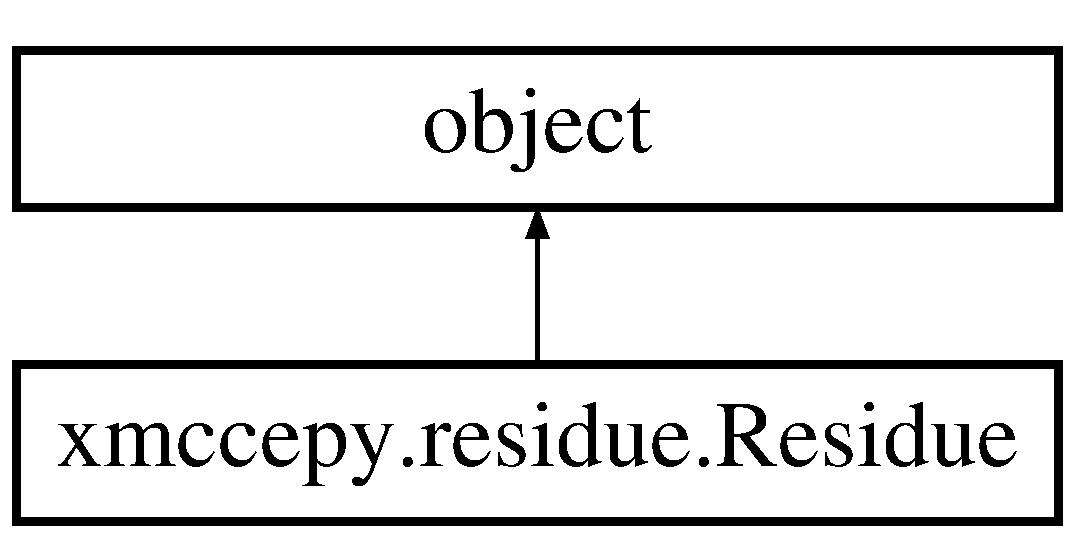
\includegraphics[height=2.000000cm]{classxmccepy_1_1residue_1_1_residue}
\end{center}
\end{figure}
\subsection*{Public Member Functions}
\begin{DoxyCompactItemize}
\item 
def \hyperlink{classxmccepy_1_1residue_1_1_residue_ab61144d8c5aed99cc706225b17e9ac03}{\-\_\-\-\_\-init\-\_\-\-\_\-}
\begin{DoxyCompactList}\small\item\em Constructor. \end{DoxyCompactList}\end{DoxyCompactItemize}
\subsection*{Public Attributes}
\begin{DoxyCompactItemize}
\item 
\hyperlink{classxmccepy_1_1residue_1_1_residue_a07eb4b463b514b1f1e86d03a6ff02a98}{res\-Name}
\item 
\hyperlink{classxmccepy_1_1residue_1_1_residue_afdd072f15f2fa5640bd67e0e5f6eb1de}{chain\-Id}
\end{DoxyCompactItemize}


\subsection{Detailed Description}
Created on Apr 1, 2014. 

\begin{DoxyAuthor}{Author}
\-: xzhu \begin{DoxyVerb}Residue class.\end{DoxyVerb}
 
\end{DoxyAuthor}


\subsection{Constructor \& Destructor Documentation}
\hypertarget{classxmccepy_1_1residue_1_1_residue_ab61144d8c5aed99cc706225b17e9ac03}{\index{xmccepy\-::residue\-::\-Residue@{xmccepy\-::residue\-::\-Residue}!\-\_\-\-\_\-init\-\_\-\-\_\-@{\-\_\-\-\_\-init\-\_\-\-\_\-}}
\index{\-\_\-\-\_\-init\-\_\-\-\_\-@{\-\_\-\-\_\-init\-\_\-\-\_\-}!xmccepy::residue::Residue@{xmccepy\-::residue\-::\-Residue}}
\subsubsection[{\-\_\-\-\_\-init\-\_\-\-\_\-}]{\setlength{\rightskip}{0pt plus 5cm}def xmccepy.\-residue.\-Residue.\-\_\-\-\_\-init\-\_\-\-\_\- (
\begin{DoxyParamCaption}
\item[{}]{self}
\end{DoxyParamCaption}
)}}\label{classxmccepy_1_1residue_1_1_residue_ab61144d8c5aed99cc706225b17e9ac03}


Constructor. 



\subsection{Member Data Documentation}
\hypertarget{classxmccepy_1_1residue_1_1_residue_afdd072f15f2fa5640bd67e0e5f6eb1de}{\index{xmccepy\-::residue\-::\-Residue@{xmccepy\-::residue\-::\-Residue}!chain\-Id@{chain\-Id}}
\index{chain\-Id@{chain\-Id}!xmccepy::residue::Residue@{xmccepy\-::residue\-::\-Residue}}
\subsubsection[{chain\-Id}]{\setlength{\rightskip}{0pt plus 5cm}xmccepy.\-residue.\-Residue.\-chain\-Id}}\label{classxmccepy_1_1residue_1_1_residue_afdd072f15f2fa5640bd67e0e5f6eb1de}
\hypertarget{classxmccepy_1_1residue_1_1_residue_a07eb4b463b514b1f1e86d03a6ff02a98}{\index{xmccepy\-::residue\-::\-Residue@{xmccepy\-::residue\-::\-Residue}!res\-Name@{res\-Name}}
\index{res\-Name@{res\-Name}!xmccepy::residue::Residue@{xmccepy\-::residue\-::\-Residue}}
\subsubsection[{res\-Name}]{\setlength{\rightskip}{0pt plus 5cm}xmccepy.\-residue.\-Residue.\-res\-Name}}\label{classxmccepy_1_1residue_1_1_residue_a07eb4b463b514b1f1e86d03a6ff02a98}


The documentation for this class was generated from the following file\-:\begin{DoxyCompactItemize}
\item 
src/xmccepy/\hyperlink{residue_8py}{residue.\-py}\end{DoxyCompactItemize}

\hypertarget{classget__charge_1_1_res_pro}{\section{get\-\_\-charge.\-Res\-Pro Class Reference}
\label{classget__charge_1_1_res_pro}\index{get\-\_\-charge.\-Res\-Pro@{get\-\_\-charge.\-Res\-Pro}}
}


Get the charges of residues.  


Inheritance diagram for get\-\_\-charge.\-Res\-Pro\-:\begin{figure}[H]
\begin{center}
\leavevmode
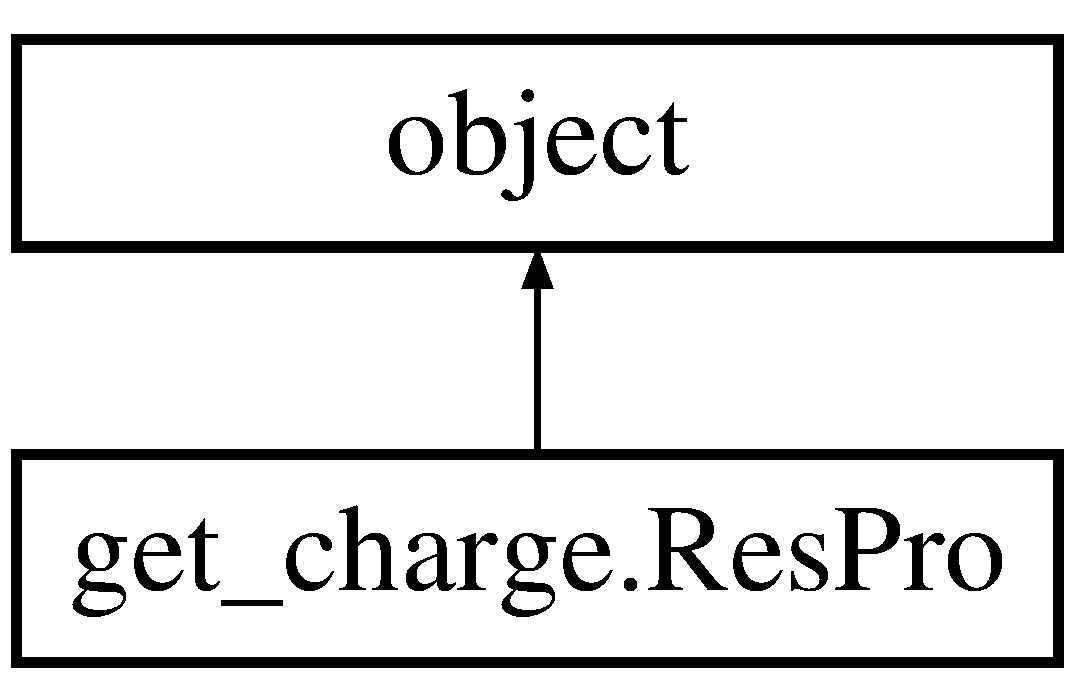
\includegraphics[height=2.000000cm]{classget__charge_1_1_res_pro}
\end{center}
\end{figure}
\subsection*{Public Member Functions}
\begin{DoxyCompactItemize}
\item 
def \hyperlink{classget__charge_1_1_res_pro_a0a1c975f9bb2ba10abe7c9f4be965b04}{\-\_\-\-\_\-init\-\_\-\-\_\-}
\item 
def \hyperlink{classget__charge_1_1_res_pro_aa0b4bed643d3d032ed97c89f5426cfef}{\-\_\-\-\_\-str\-\_\-\-\_\-}
\item 
def \hyperlink{classget__charge_1_1_res_pro_a2ff72116a5eec8e96c3085269e265250}{get\-Stat}
\end{DoxyCompactItemize}
\subsection*{Public Attributes}
\begin{DoxyCompactItemize}
\item 
\hyperlink{classget__charge_1_1_res_pro_aaa9de483c5f88fe49fd682dd1b8a62e7}{charges}
\item 
\hyperlink{classget__charge_1_1_res_pro_af00fc3f5bae5c3d3734b384b2d2c466d}{r\-Name}
\item 
\hyperlink{classget__charge_1_1_res_pro_a19649fb10b2d365eddf247107e39b0d0}{avg}
\item 
\hyperlink{classget__charge_1_1_res_pro_afad79b4ab35532abe9a7d305725fb0bc}{std}
\item 
\hyperlink{classget__charge_1_1_res_pro_a0f70c65e6cef508bcd63147ad7265fee}{protonation}
\end{DoxyCompactItemize}
\subsection*{Static Public Attributes}
\begin{DoxyCompactItemize}
\item 
tuple \hyperlink{classget__charge_1_1_res_pro_a19f4f7319d0e78071cad89e477d96f9f}{all\-Run\-Types} = (\char`\"{}cqr\char`\"{}, \char`\"{}cql\char`\"{}, \char`\"{}cdr\char`\"{}, \char`\"{}cdl\char`\"{}, \char`\"{}hqr\char`\"{}, \char`\"{}hql\char`\"{}, \char`\"{}hdr\char`\"{}, \char`\"{}hdl\char`\"{})
\item 
string \hyperlink{classget__charge_1_1_res_pro_a6abe27b9c2d55e6f735eb1afe0a83916}{D\-E\-F\-A\-U\-L\-T\-\_\-\-C\-R\-G} = \char`\"{}na\char`\"{}
\end{DoxyCompactItemize}
\subsection*{Static Private Attributes}
\begin{DoxyCompactItemize}
\item 
\hyperlink{classget__charge_1_1_res_pro_a2d6a3912943f7b858e8b5f04231c3420}{\-\_\-\-\_\-repr\-\_\-\-\_\-} = \hyperlink{classget__charge_1_1_res_pro_aa0b4bed643d3d032ed97c89f5426cfef}{\-\_\-\-\_\-str\-\_\-\-\_\-}
\end{DoxyCompactItemize}


\subsection{Detailed Description}
Get the charges of residues. 

It's similar to the script \char`\"{}collect\-\_\-crg.\-py\char`\"{}. 

\subsection{Constructor \& Destructor Documentation}
\hypertarget{classget__charge_1_1_res_pro_a0a1c975f9bb2ba10abe7c9f4be965b04}{\index{get\-\_\-charge\-::\-Res\-Pro@{get\-\_\-charge\-::\-Res\-Pro}!\-\_\-\-\_\-init\-\_\-\-\_\-@{\-\_\-\-\_\-init\-\_\-\-\_\-}}
\index{\-\_\-\-\_\-init\-\_\-\-\_\-@{\-\_\-\-\_\-init\-\_\-\-\_\-}!get_charge::ResPro@{get\-\_\-charge\-::\-Res\-Pro}}
\subsubsection[{\-\_\-\-\_\-init\-\_\-\-\_\-}]{\setlength{\rightskip}{0pt plus 5cm}def get\-\_\-charge.\-Res\-Pro.\-\_\-\-\_\-init\-\_\-\-\_\- (
\begin{DoxyParamCaption}
\item[{}]{self, }
\item[{}]{name = {\ttfamily ''}}
\end{DoxyParamCaption}
)}}\label{classget__charge_1_1_res_pro_a0a1c975f9bb2ba10abe7c9f4be965b04}


\subsection{Member Function Documentation}
\hypertarget{classget__charge_1_1_res_pro_aa0b4bed643d3d032ed97c89f5426cfef}{\index{get\-\_\-charge\-::\-Res\-Pro@{get\-\_\-charge\-::\-Res\-Pro}!\-\_\-\-\_\-str\-\_\-\-\_\-@{\-\_\-\-\_\-str\-\_\-\-\_\-}}
\index{\-\_\-\-\_\-str\-\_\-\-\_\-@{\-\_\-\-\_\-str\-\_\-\-\_\-}!get_charge::ResPro@{get\-\_\-charge\-::\-Res\-Pro}}
\subsubsection[{\-\_\-\-\_\-str\-\_\-\-\_\-}]{\setlength{\rightskip}{0pt plus 5cm}def get\-\_\-charge.\-Res\-Pro.\-\_\-\-\_\-str\-\_\-\-\_\- (
\begin{DoxyParamCaption}
\item[{}]{self}
\end{DoxyParamCaption}
)}}\label{classget__charge_1_1_res_pro_aa0b4bed643d3d032ed97c89f5426cfef}
\hypertarget{classget__charge_1_1_res_pro_a2ff72116a5eec8e96c3085269e265250}{\index{get\-\_\-charge\-::\-Res\-Pro@{get\-\_\-charge\-::\-Res\-Pro}!get\-Stat@{get\-Stat}}
\index{get\-Stat@{get\-Stat}!get_charge::ResPro@{get\-\_\-charge\-::\-Res\-Pro}}
\subsubsection[{get\-Stat}]{\setlength{\rightskip}{0pt plus 5cm}def get\-\_\-charge.\-Res\-Pro.\-get\-Stat (
\begin{DoxyParamCaption}
\item[{}]{self}
\end{DoxyParamCaption}
)}}\label{classget__charge_1_1_res_pro_a2ff72116a5eec8e96c3085269e265250}


\subsection{Member Data Documentation}
\hypertarget{classget__charge_1_1_res_pro_a2d6a3912943f7b858e8b5f04231c3420}{\index{get\-\_\-charge\-::\-Res\-Pro@{get\-\_\-charge\-::\-Res\-Pro}!\-\_\-\-\_\-repr\-\_\-\-\_\-@{\-\_\-\-\_\-repr\-\_\-\-\_\-}}
\index{\-\_\-\-\_\-repr\-\_\-\-\_\-@{\-\_\-\-\_\-repr\-\_\-\-\_\-}!get_charge::ResPro@{get\-\_\-charge\-::\-Res\-Pro}}
\subsubsection[{\-\_\-\-\_\-repr\-\_\-\-\_\-}]{\setlength{\rightskip}{0pt plus 5cm}get\-\_\-charge.\-Res\-Pro.\-\_\-\-\_\-repr\-\_\-\-\_\- = {\bf \-\_\-\-\_\-str\-\_\-\-\_\-}\hspace{0.3cm}{\ttfamily [static]}, {\ttfamily [private]}}}\label{classget__charge_1_1_res_pro_a2d6a3912943f7b858e8b5f04231c3420}
\hypertarget{classget__charge_1_1_res_pro_a19f4f7319d0e78071cad89e477d96f9f}{\index{get\-\_\-charge\-::\-Res\-Pro@{get\-\_\-charge\-::\-Res\-Pro}!all\-Run\-Types@{all\-Run\-Types}}
\index{all\-Run\-Types@{all\-Run\-Types}!get_charge::ResPro@{get\-\_\-charge\-::\-Res\-Pro}}
\subsubsection[{all\-Run\-Types}]{\setlength{\rightskip}{0pt plus 5cm}tuple get\-\_\-charge.\-Res\-Pro.\-all\-Run\-Types = (\char`\"{}cqr\char`\"{}, \char`\"{}cql\char`\"{}, \char`\"{}cdr\char`\"{}, \char`\"{}cdl\char`\"{}, \char`\"{}hqr\char`\"{}, \char`\"{}hql\char`\"{}, \char`\"{}hdr\char`\"{}, \char`\"{}hdl\char`\"{})\hspace{0.3cm}{\ttfamily [static]}}}\label{classget__charge_1_1_res_pro_a19f4f7319d0e78071cad89e477d96f9f}
\hypertarget{classget__charge_1_1_res_pro_a19649fb10b2d365eddf247107e39b0d0}{\index{get\-\_\-charge\-::\-Res\-Pro@{get\-\_\-charge\-::\-Res\-Pro}!avg@{avg}}
\index{avg@{avg}!get_charge::ResPro@{get\-\_\-charge\-::\-Res\-Pro}}
\subsubsection[{avg}]{\setlength{\rightskip}{0pt plus 5cm}get\-\_\-charge.\-Res\-Pro.\-avg}}\label{classget__charge_1_1_res_pro_a19649fb10b2d365eddf247107e39b0d0}
\hypertarget{classget__charge_1_1_res_pro_aaa9de483c5f88fe49fd682dd1b8a62e7}{\index{get\-\_\-charge\-::\-Res\-Pro@{get\-\_\-charge\-::\-Res\-Pro}!charges@{charges}}
\index{charges@{charges}!get_charge::ResPro@{get\-\_\-charge\-::\-Res\-Pro}}
\subsubsection[{charges}]{\setlength{\rightskip}{0pt plus 5cm}get\-\_\-charge.\-Res\-Pro.\-charges}}\label{classget__charge_1_1_res_pro_aaa9de483c5f88fe49fd682dd1b8a62e7}
\hypertarget{classget__charge_1_1_res_pro_a6abe27b9c2d55e6f735eb1afe0a83916}{\index{get\-\_\-charge\-::\-Res\-Pro@{get\-\_\-charge\-::\-Res\-Pro}!D\-E\-F\-A\-U\-L\-T\-\_\-\-C\-R\-G@{D\-E\-F\-A\-U\-L\-T\-\_\-\-C\-R\-G}}
\index{D\-E\-F\-A\-U\-L\-T\-\_\-\-C\-R\-G@{D\-E\-F\-A\-U\-L\-T\-\_\-\-C\-R\-G}!get_charge::ResPro@{get\-\_\-charge\-::\-Res\-Pro}}
\subsubsection[{D\-E\-F\-A\-U\-L\-T\-\_\-\-C\-R\-G}]{\setlength{\rightskip}{0pt plus 5cm}string get\-\_\-charge.\-Res\-Pro.\-D\-E\-F\-A\-U\-L\-T\-\_\-\-C\-R\-G = \char`\"{}na\char`\"{}\hspace{0.3cm}{\ttfamily [static]}}}\label{classget__charge_1_1_res_pro_a6abe27b9c2d55e6f735eb1afe0a83916}
\hypertarget{classget__charge_1_1_res_pro_a0f70c65e6cef508bcd63147ad7265fee}{\index{get\-\_\-charge\-::\-Res\-Pro@{get\-\_\-charge\-::\-Res\-Pro}!protonation@{protonation}}
\index{protonation@{protonation}!get_charge::ResPro@{get\-\_\-charge\-::\-Res\-Pro}}
\subsubsection[{protonation}]{\setlength{\rightskip}{0pt plus 5cm}get\-\_\-charge.\-Res\-Pro.\-protonation}}\label{classget__charge_1_1_res_pro_a0f70c65e6cef508bcd63147ad7265fee}
\hypertarget{classget__charge_1_1_res_pro_af00fc3f5bae5c3d3734b384b2d2c466d}{\index{get\-\_\-charge\-::\-Res\-Pro@{get\-\_\-charge\-::\-Res\-Pro}!r\-Name@{r\-Name}}
\index{r\-Name@{r\-Name}!get_charge::ResPro@{get\-\_\-charge\-::\-Res\-Pro}}
\subsubsection[{r\-Name}]{\setlength{\rightskip}{0pt plus 5cm}get\-\_\-charge.\-Res\-Pro.\-r\-Name}}\label{classget__charge_1_1_res_pro_af00fc3f5bae5c3d3734b384b2d2c466d}
\hypertarget{classget__charge_1_1_res_pro_afad79b4ab35532abe9a7d305725fb0bc}{\index{get\-\_\-charge\-::\-Res\-Pro@{get\-\_\-charge\-::\-Res\-Pro}!std@{std}}
\index{std@{std}!get_charge::ResPro@{get\-\_\-charge\-::\-Res\-Pro}}
\subsubsection[{std}]{\setlength{\rightskip}{0pt plus 5cm}get\-\_\-charge.\-Res\-Pro.\-std}}\label{classget__charge_1_1_res_pro_afad79b4ab35532abe9a7d305725fb0bc}


The documentation for this class was generated from the following file\-:\begin{DoxyCompactItemize}
\item 
src/scripts/mcce/\hyperlink{get__charge_8py}{get\-\_\-charge.\-py}\end{DoxyCompactItemize}

\hypertarget{classcollect__crg_1_1_res_pro}{\section{collect\-\_\-crg.\-Res\-Pro Class Reference}
\label{classcollect__crg_1_1_res_pro}\index{collect\-\_\-crg.\-Res\-Pro@{collect\-\_\-crg.\-Res\-Pro}}
}


Residue class.  


Inheritance diagram for collect\-\_\-crg.\-Res\-Pro\-:\begin{figure}[H]
\begin{center}
\leavevmode
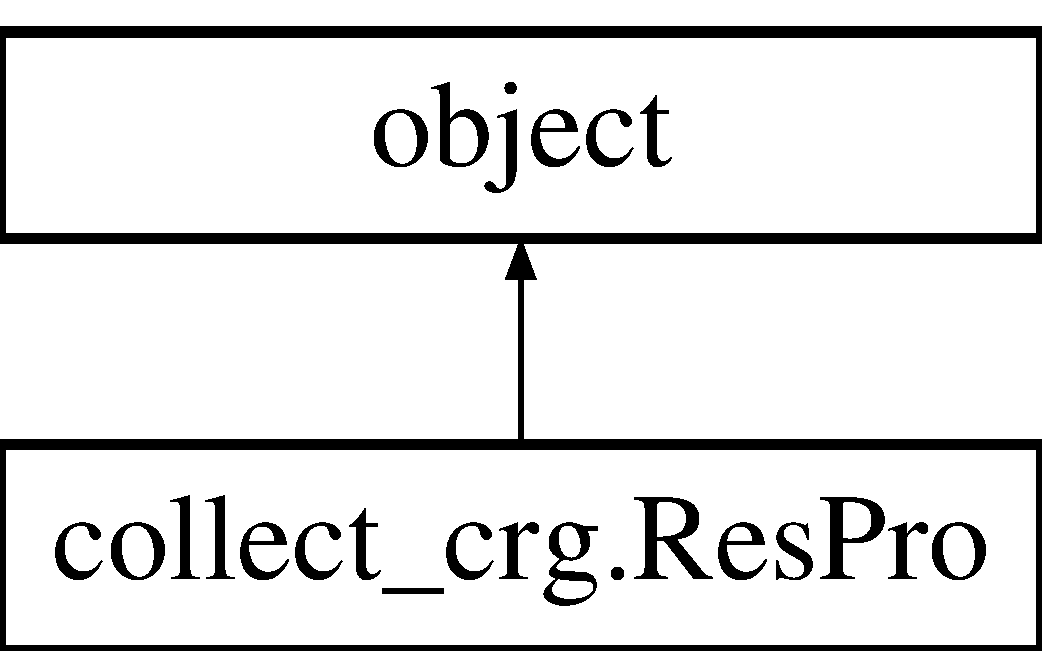
\includegraphics[height=2.000000cm]{classcollect__crg_1_1_res_pro}
\end{center}
\end{figure}
\subsection*{Public Member Functions}
\begin{DoxyCompactItemize}
\item 
def \hyperlink{classcollect__crg_1_1_res_pro_ab563227610708f8c5867c766b3b7d3e9}{\-\_\-\-\_\-init\-\_\-\-\_\-}
\item 
def \hyperlink{classcollect__crg_1_1_res_pro_ac4141791c8bd45b3ffe8b5ec2483bfc1}{\-\_\-\-\_\-str\-\_\-\-\_\-}
\end{DoxyCompactItemize}
\subsection*{Public Attributes}
\begin{DoxyCompactItemize}
\item 
\hyperlink{classcollect__crg_1_1_res_pro_a7075290e45b0608bb59ebfe42722b4e3}{charges}
\item 
\hyperlink{classcollect__crg_1_1_res_pro_aec2b2fecfffa4aa7728013ee504d48f7}{r\-Name}
\end{DoxyCompactItemize}
\subsection*{Static Public Attributes}
\begin{DoxyCompactItemize}
\item 
tuple \hyperlink{classcollect__crg_1_1_res_pro_a0978c5440914518afa5bba719a40bfa1}{all\-Run\-Types} = (\char`\"{}cqr\char`\"{}, \char`\"{}cql\char`\"{}, \char`\"{}cdr\char`\"{}, \char`\"{}cdl\char`\"{}, \char`\"{}hqr\char`\"{}, \char`\"{}hql\char`\"{}, \char`\"{}hdr\char`\"{}, \char`\"{}hdl\char`\"{})
\end{DoxyCompactItemize}
\subsection*{Static Private Attributes}
\begin{DoxyCompactItemize}
\item 
\hyperlink{classcollect__crg_1_1_res_pro_ab775338960aae2ea56892e7a39a6e63c}{\-\_\-\-\_\-repr\-\_\-\-\_\-} = \hyperlink{classcollect__crg_1_1_res_pro_ac4141791c8bd45b3ffe8b5ec2483bfc1}{\-\_\-\-\_\-str\-\_\-\-\_\-}
\end{DoxyCompactItemize}


\subsection{Detailed Description}
Residue class. 

It only contains the charges of the residues in different types of runs. 

\subsection{Constructor \& Destructor Documentation}
\hypertarget{classcollect__crg_1_1_res_pro_ab563227610708f8c5867c766b3b7d3e9}{\index{collect\-\_\-crg\-::\-Res\-Pro@{collect\-\_\-crg\-::\-Res\-Pro}!\-\_\-\-\_\-init\-\_\-\-\_\-@{\-\_\-\-\_\-init\-\_\-\-\_\-}}
\index{\-\_\-\-\_\-init\-\_\-\-\_\-@{\-\_\-\-\_\-init\-\_\-\-\_\-}!collect_crg::ResPro@{collect\-\_\-crg\-::\-Res\-Pro}}
\subsubsection[{\-\_\-\-\_\-init\-\_\-\-\_\-}]{\setlength{\rightskip}{0pt plus 5cm}def collect\-\_\-crg.\-Res\-Pro.\-\_\-\-\_\-init\-\_\-\-\_\- (
\begin{DoxyParamCaption}
\item[{}]{self, }
\item[{}]{name = {\ttfamily ''}}
\end{DoxyParamCaption}
)}}\label{classcollect__crg_1_1_res_pro_ab563227610708f8c5867c766b3b7d3e9}


\subsection{Member Function Documentation}
\hypertarget{classcollect__crg_1_1_res_pro_ac4141791c8bd45b3ffe8b5ec2483bfc1}{\index{collect\-\_\-crg\-::\-Res\-Pro@{collect\-\_\-crg\-::\-Res\-Pro}!\-\_\-\-\_\-str\-\_\-\-\_\-@{\-\_\-\-\_\-str\-\_\-\-\_\-}}
\index{\-\_\-\-\_\-str\-\_\-\-\_\-@{\-\_\-\-\_\-str\-\_\-\-\_\-}!collect_crg::ResPro@{collect\-\_\-crg\-::\-Res\-Pro}}
\subsubsection[{\-\_\-\-\_\-str\-\_\-\-\_\-}]{\setlength{\rightskip}{0pt plus 5cm}def collect\-\_\-crg.\-Res\-Pro.\-\_\-\-\_\-str\-\_\-\-\_\- (
\begin{DoxyParamCaption}
\item[{}]{self}
\end{DoxyParamCaption}
)}}\label{classcollect__crg_1_1_res_pro_ac4141791c8bd45b3ffe8b5ec2483bfc1}


\subsection{Member Data Documentation}
\hypertarget{classcollect__crg_1_1_res_pro_ab775338960aae2ea56892e7a39a6e63c}{\index{collect\-\_\-crg\-::\-Res\-Pro@{collect\-\_\-crg\-::\-Res\-Pro}!\-\_\-\-\_\-repr\-\_\-\-\_\-@{\-\_\-\-\_\-repr\-\_\-\-\_\-}}
\index{\-\_\-\-\_\-repr\-\_\-\-\_\-@{\-\_\-\-\_\-repr\-\_\-\-\_\-}!collect_crg::ResPro@{collect\-\_\-crg\-::\-Res\-Pro}}
\subsubsection[{\-\_\-\-\_\-repr\-\_\-\-\_\-}]{\setlength{\rightskip}{0pt plus 5cm}collect\-\_\-crg.\-Res\-Pro.\-\_\-\-\_\-repr\-\_\-\-\_\- = {\bf \-\_\-\-\_\-str\-\_\-\-\_\-}\hspace{0.3cm}{\ttfamily [static]}, {\ttfamily [private]}}}\label{classcollect__crg_1_1_res_pro_ab775338960aae2ea56892e7a39a6e63c}
\hypertarget{classcollect__crg_1_1_res_pro_a0978c5440914518afa5bba719a40bfa1}{\index{collect\-\_\-crg\-::\-Res\-Pro@{collect\-\_\-crg\-::\-Res\-Pro}!all\-Run\-Types@{all\-Run\-Types}}
\index{all\-Run\-Types@{all\-Run\-Types}!collect_crg::ResPro@{collect\-\_\-crg\-::\-Res\-Pro}}
\subsubsection[{all\-Run\-Types}]{\setlength{\rightskip}{0pt plus 5cm}tuple collect\-\_\-crg.\-Res\-Pro.\-all\-Run\-Types = (\char`\"{}cqr\char`\"{}, \char`\"{}cql\char`\"{}, \char`\"{}cdr\char`\"{}, \char`\"{}cdl\char`\"{}, \char`\"{}hqr\char`\"{}, \char`\"{}hql\char`\"{}, \char`\"{}hdr\char`\"{}, \char`\"{}hdl\char`\"{})\hspace{0.3cm}{\ttfamily [static]}}}\label{classcollect__crg_1_1_res_pro_a0978c5440914518afa5bba719a40bfa1}
\hypertarget{classcollect__crg_1_1_res_pro_a7075290e45b0608bb59ebfe42722b4e3}{\index{collect\-\_\-crg\-::\-Res\-Pro@{collect\-\_\-crg\-::\-Res\-Pro}!charges@{charges}}
\index{charges@{charges}!collect_crg::ResPro@{collect\-\_\-crg\-::\-Res\-Pro}}
\subsubsection[{charges}]{\setlength{\rightskip}{0pt plus 5cm}collect\-\_\-crg.\-Res\-Pro.\-charges}}\label{classcollect__crg_1_1_res_pro_a7075290e45b0608bb59ebfe42722b4e3}
\hypertarget{classcollect__crg_1_1_res_pro_aec2b2fecfffa4aa7728013ee504d48f7}{\index{collect\-\_\-crg\-::\-Res\-Pro@{collect\-\_\-crg\-::\-Res\-Pro}!r\-Name@{r\-Name}}
\index{r\-Name@{r\-Name}!collect_crg::ResPro@{collect\-\_\-crg\-::\-Res\-Pro}}
\subsubsection[{r\-Name}]{\setlength{\rightskip}{0pt plus 5cm}collect\-\_\-crg.\-Res\-Pro.\-r\-Name}}\label{classcollect__crg_1_1_res_pro_aec2b2fecfffa4aa7728013ee504d48f7}


The documentation for this class was generated from the following file\-:\begin{DoxyCompactItemize}
\item 
src/scripts/mcce/\hyperlink{collect__crg_8py}{collect\-\_\-crg.\-py}\end{DoxyCompactItemize}

\hypertarget{classtest__residue_1_1_test}{\section{test\-\_\-residue.\-Test Class Reference}
\label{classtest__residue_1_1_test}\index{test\-\_\-residue.\-Test@{test\-\_\-residue.\-Test}}
}
Inheritance diagram for test\-\_\-residue.\-Test\-:\begin{figure}[H]
\begin{center}
\leavevmode
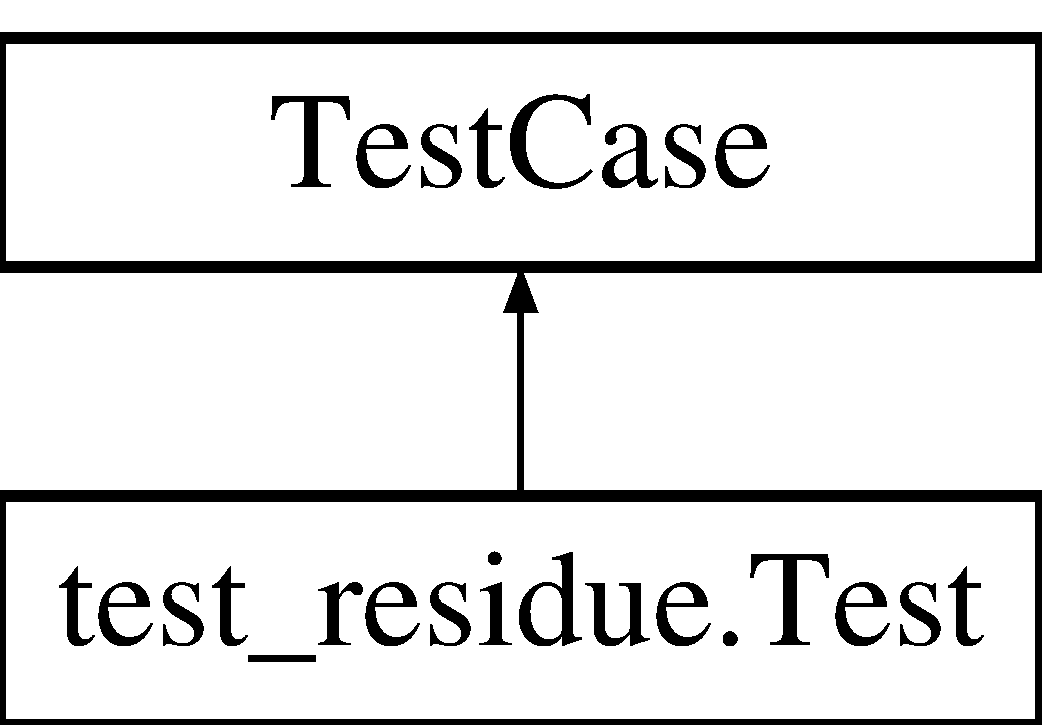
\includegraphics[height=2.000000cm]{classtest__residue_1_1_test}
\end{center}
\end{figure}
\subsection*{Public Member Functions}
\begin{DoxyCompactItemize}
\item 
def \hyperlink{classtest__residue_1_1_test_a3de9cc2e1207c57440fe254a327281cb}{set\-Up}
\item 
def \hyperlink{classtest__residue_1_1_test_aba3d56bc2acc6cb69c43946674b14807}{tear\-Down}
\item 
def \hyperlink{classtest__residue_1_1_test_a1f1b4ac54488dab8d9449a7ea70891e0}{test\-\_\-name}
\end{DoxyCompactItemize}
\subsection*{Public Attributes}
\begin{DoxyCompactItemize}
\item 
\hyperlink{classtest__residue_1_1_test_a86d05f73c4c2a2aa36049ed550f22877}{r}
\end{DoxyCompactItemize}


\subsection{Member Function Documentation}
\hypertarget{classtest__residue_1_1_test_a3de9cc2e1207c57440fe254a327281cb}{\index{test\-\_\-residue\-::\-Test@{test\-\_\-residue\-::\-Test}!set\-Up@{set\-Up}}
\index{set\-Up@{set\-Up}!test_residue::Test@{test\-\_\-residue\-::\-Test}}
\subsubsection[{set\-Up}]{\setlength{\rightskip}{0pt plus 5cm}def test\-\_\-residue.\-Test.\-set\-Up (
\begin{DoxyParamCaption}
\item[{}]{self}
\end{DoxyParamCaption}
)}}\label{classtest__residue_1_1_test_a3de9cc2e1207c57440fe254a327281cb}
\hypertarget{classtest__residue_1_1_test_aba3d56bc2acc6cb69c43946674b14807}{\index{test\-\_\-residue\-::\-Test@{test\-\_\-residue\-::\-Test}!tear\-Down@{tear\-Down}}
\index{tear\-Down@{tear\-Down}!test_residue::Test@{test\-\_\-residue\-::\-Test}}
\subsubsection[{tear\-Down}]{\setlength{\rightskip}{0pt plus 5cm}def test\-\_\-residue.\-Test.\-tear\-Down (
\begin{DoxyParamCaption}
\item[{}]{self}
\end{DoxyParamCaption}
)}}\label{classtest__residue_1_1_test_aba3d56bc2acc6cb69c43946674b14807}
\hypertarget{classtest__residue_1_1_test_a1f1b4ac54488dab8d9449a7ea70891e0}{\index{test\-\_\-residue\-::\-Test@{test\-\_\-residue\-::\-Test}!test\-\_\-name@{test\-\_\-name}}
\index{test\-\_\-name@{test\-\_\-name}!test_residue::Test@{test\-\_\-residue\-::\-Test}}
\subsubsection[{test\-\_\-name}]{\setlength{\rightskip}{0pt plus 5cm}def test\-\_\-residue.\-Test.\-test\-\_\-name (
\begin{DoxyParamCaption}
\item[{}]{self}
\end{DoxyParamCaption}
)}}\label{classtest__residue_1_1_test_a1f1b4ac54488dab8d9449a7ea70891e0}


\subsection{Member Data Documentation}
\hypertarget{classtest__residue_1_1_test_a86d05f73c4c2a2aa36049ed550f22877}{\index{test\-\_\-residue\-::\-Test@{test\-\_\-residue\-::\-Test}!r@{r}}
\index{r@{r}!test_residue::Test@{test\-\_\-residue\-::\-Test}}
\subsubsection[{r}]{\setlength{\rightskip}{0pt plus 5cm}test\-\_\-residue.\-Test.\-r}}\label{classtest__residue_1_1_test_a86d05f73c4c2a2aa36049ed550f22877}


The documentation for this class was generated from the following file\-:\begin{DoxyCompactItemize}
\item 
src/test/test\-\_\-xmccepy/\hyperlink{test__residue_8py}{test\-\_\-residue.\-py}\end{DoxyCompactItemize}

\hypertarget{classtest__atom_1_1_test}{\section{test\-\_\-atom.\-Test Class Reference}
\label{classtest__atom_1_1_test}\index{test\-\_\-atom.\-Test@{test\-\_\-atom.\-Test}}
}
Inheritance diagram for test\-\_\-atom.\-Test\-:\begin{figure}[H]
\begin{center}
\leavevmode
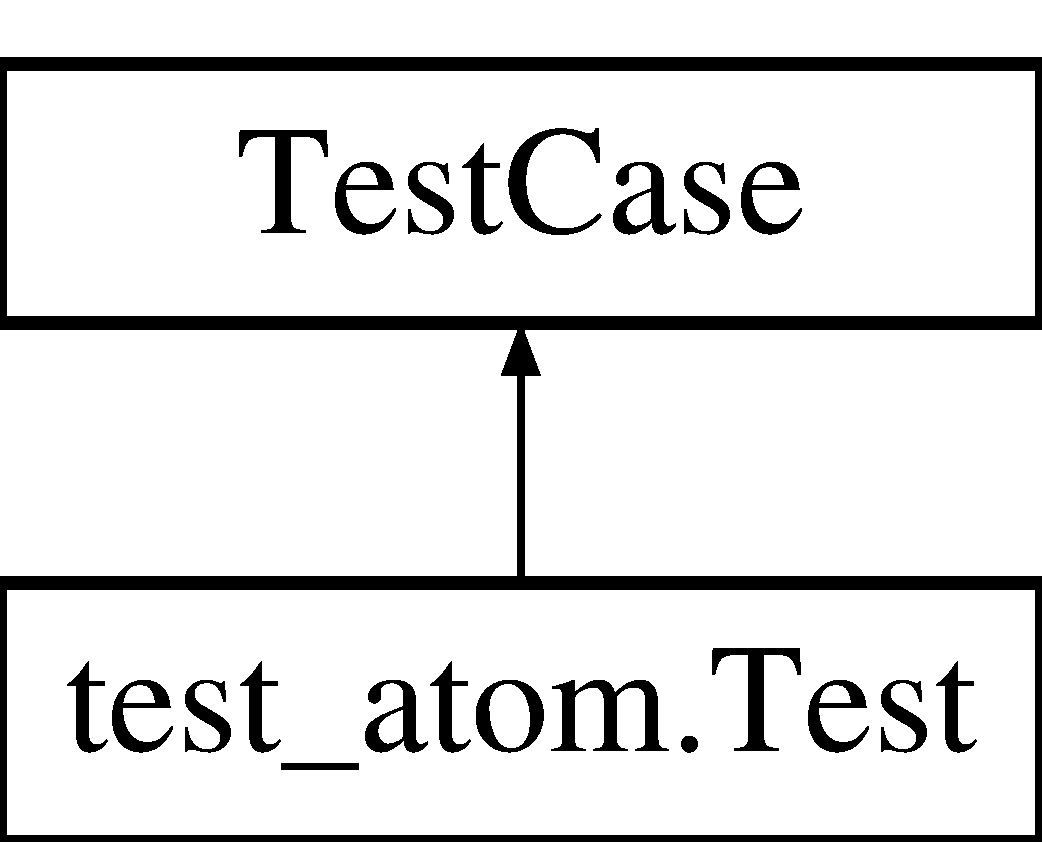
\includegraphics[height=2.000000cm]{classtest__atom_1_1_test}
\end{center}
\end{figure}
\subsection*{Public Member Functions}
\begin{DoxyCompactItemize}
\item 
def \hyperlink{classtest__atom_1_1_test_aeec0dbbe10167d3d723e68bb89533cd1}{set\-Up}
\item 
def \hyperlink{classtest__atom_1_1_test_ac516b539f9a0a060a4391539603b643e}{tear\-Down}
\item 
def \hyperlink{classtest__atom_1_1_test_acb79481dc2bf3d9f569075a8f71dcce1}{test\-\_\-atom}
\item 
def \hyperlink{classtest__atom_1_1_test_ac36221e3dd8e2e7c9318d3af919edd6d}{test\-\_\-read\-Step1\-Line}
\end{DoxyCompactItemize}
\subsection*{Public Attributes}
\begin{DoxyCompactItemize}
\item 
\hyperlink{classtest__atom_1_1_test_a6ab6843fb798ca4f1d2c6f3315204768}{a}
\end{DoxyCompactItemize}


\subsection{Member Function Documentation}
\hypertarget{classtest__atom_1_1_test_aeec0dbbe10167d3d723e68bb89533cd1}{\index{test\-\_\-atom\-::\-Test@{test\-\_\-atom\-::\-Test}!set\-Up@{set\-Up}}
\index{set\-Up@{set\-Up}!test_atom::Test@{test\-\_\-atom\-::\-Test}}
\subsubsection[{set\-Up}]{\setlength{\rightskip}{0pt plus 5cm}def test\-\_\-atom.\-Test.\-set\-Up (
\begin{DoxyParamCaption}
\item[{}]{self}
\end{DoxyParamCaption}
)}}\label{classtest__atom_1_1_test_aeec0dbbe10167d3d723e68bb89533cd1}
\hypertarget{classtest__atom_1_1_test_ac516b539f9a0a060a4391539603b643e}{\index{test\-\_\-atom\-::\-Test@{test\-\_\-atom\-::\-Test}!tear\-Down@{tear\-Down}}
\index{tear\-Down@{tear\-Down}!test_atom::Test@{test\-\_\-atom\-::\-Test}}
\subsubsection[{tear\-Down}]{\setlength{\rightskip}{0pt plus 5cm}def test\-\_\-atom.\-Test.\-tear\-Down (
\begin{DoxyParamCaption}
\item[{}]{self}
\end{DoxyParamCaption}
)}}\label{classtest__atom_1_1_test_ac516b539f9a0a060a4391539603b643e}
\hypertarget{classtest__atom_1_1_test_acb79481dc2bf3d9f569075a8f71dcce1}{\index{test\-\_\-atom\-::\-Test@{test\-\_\-atom\-::\-Test}!test\-\_\-atom@{test\-\_\-atom}}
\index{test\-\_\-atom@{test\-\_\-atom}!test_atom::Test@{test\-\_\-atom\-::\-Test}}
\subsubsection[{test\-\_\-atom}]{\setlength{\rightskip}{0pt plus 5cm}def test\-\_\-atom.\-Test.\-test\-\_\-atom (
\begin{DoxyParamCaption}
\item[{}]{self}
\end{DoxyParamCaption}
)}}\label{classtest__atom_1_1_test_acb79481dc2bf3d9f569075a8f71dcce1}
\hypertarget{classtest__atom_1_1_test_ac36221e3dd8e2e7c9318d3af919edd6d}{\index{test\-\_\-atom\-::\-Test@{test\-\_\-atom\-::\-Test}!test\-\_\-read\-Step1\-Line@{test\-\_\-read\-Step1\-Line}}
\index{test\-\_\-read\-Step1\-Line@{test\-\_\-read\-Step1\-Line}!test_atom::Test@{test\-\_\-atom\-::\-Test}}
\subsubsection[{test\-\_\-read\-Step1\-Line}]{\setlength{\rightskip}{0pt plus 5cm}def test\-\_\-atom.\-Test.\-test\-\_\-read\-Step1\-Line (
\begin{DoxyParamCaption}
\item[{}]{self}
\end{DoxyParamCaption}
)}}\label{classtest__atom_1_1_test_ac36221e3dd8e2e7c9318d3af919edd6d}


\subsection{Member Data Documentation}
\hypertarget{classtest__atom_1_1_test_a6ab6843fb798ca4f1d2c6f3315204768}{\index{test\-\_\-atom\-::\-Test@{test\-\_\-atom\-::\-Test}!a@{a}}
\index{a@{a}!test_atom::Test@{test\-\_\-atom\-::\-Test}}
\subsubsection[{a}]{\setlength{\rightskip}{0pt plus 5cm}test\-\_\-atom.\-Test.\-a}}\label{classtest__atom_1_1_test_a6ab6843fb798ca4f1d2c6f3315204768}


The documentation for this class was generated from the following file\-:\begin{DoxyCompactItemize}
\item 
src/test/test\-\_\-xmccepy/\hyperlink{test__atom_8py}{test\-\_\-atom.\-py}\end{DoxyCompactItemize}

\hypertarget{classcomp__desol_1_1_water_conf}{\section{comp\-\_\-desol.\-Water\-Conf Class Reference}
\label{classcomp__desol_1_1_water_conf}\index{comp\-\_\-desol.\-Water\-Conf@{comp\-\_\-desol.\-Water\-Conf}}
}


Compare the desolvation energies of waters.  


Inheritance diagram for comp\-\_\-desol.\-Water\-Conf\-:\begin{figure}[H]
\begin{center}
\leavevmode
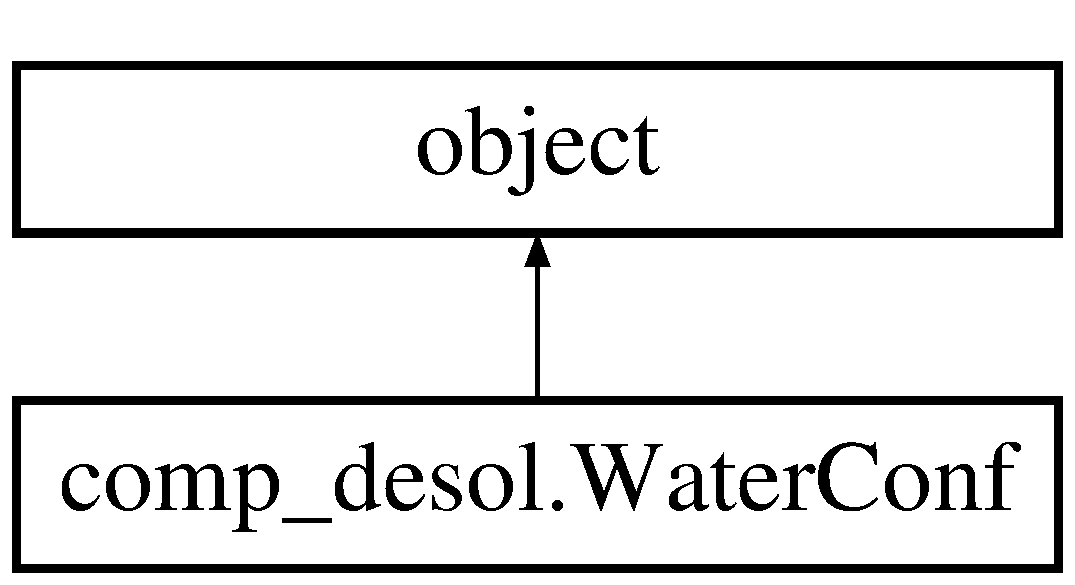
\includegraphics[height=2.000000cm]{classcomp__desol_1_1_water_conf}
\end{center}
\end{figure}
\subsection*{Public Member Functions}
\begin{DoxyCompactItemize}
\item 
def \hyperlink{classcomp__desol_1_1_water_conf_a0fb421de7d4a112769e5da6004c51b93}{\-\_\-\-\_\-init\-\_\-\-\_\-}
\end{DoxyCompactItemize}
\subsection*{Public Attributes}
\begin{DoxyCompactItemize}
\item 
\hyperlink{classcomp__desol_1_1_water_conf_a5b1921836f354b358be05d4ea6b93ae6}{conf\-Name}
\item 
\hyperlink{classcomp__desol_1_1_water_conf_aaf4a467d6793dea2e163ba5e7aa1888c}{desolv}
\end{DoxyCompactItemize}


\subsection{Detailed Description}
Compare the desolvation energies of waters. 

Water conformer class. 

\subsection{Constructor \& Destructor Documentation}
\hypertarget{classcomp__desol_1_1_water_conf_a0fb421de7d4a112769e5da6004c51b93}{\index{comp\-\_\-desol\-::\-Water\-Conf@{comp\-\_\-desol\-::\-Water\-Conf}!\-\_\-\-\_\-init\-\_\-\-\_\-@{\-\_\-\-\_\-init\-\_\-\-\_\-}}
\index{\-\_\-\-\_\-init\-\_\-\-\_\-@{\-\_\-\-\_\-init\-\_\-\-\_\-}!comp_desol::WaterConf@{comp\-\_\-desol\-::\-Water\-Conf}}
\subsubsection[{\-\_\-\-\_\-init\-\_\-\-\_\-}]{\setlength{\rightskip}{0pt plus 5cm}def comp\-\_\-desol.\-Water\-Conf.\-\_\-\-\_\-init\-\_\-\-\_\- (
\begin{DoxyParamCaption}
\item[{}]{self}
\end{DoxyParamCaption}
)}}\label{classcomp__desol_1_1_water_conf_a0fb421de7d4a112769e5da6004c51b93}


\subsection{Member Data Documentation}
\hypertarget{classcomp__desol_1_1_water_conf_a5b1921836f354b358be05d4ea6b93ae6}{\index{comp\-\_\-desol\-::\-Water\-Conf@{comp\-\_\-desol\-::\-Water\-Conf}!conf\-Name@{conf\-Name}}
\index{conf\-Name@{conf\-Name}!comp_desol::WaterConf@{comp\-\_\-desol\-::\-Water\-Conf}}
\subsubsection[{conf\-Name}]{\setlength{\rightskip}{0pt plus 5cm}comp\-\_\-desol.\-Water\-Conf.\-conf\-Name}}\label{classcomp__desol_1_1_water_conf_a5b1921836f354b358be05d4ea6b93ae6}
\hypertarget{classcomp__desol_1_1_water_conf_aaf4a467d6793dea2e163ba5e7aa1888c}{\index{comp\-\_\-desol\-::\-Water\-Conf@{comp\-\_\-desol\-::\-Water\-Conf}!desolv@{desolv}}
\index{desolv@{desolv}!comp_desol::WaterConf@{comp\-\_\-desol\-::\-Water\-Conf}}
\subsubsection[{desolv}]{\setlength{\rightskip}{0pt plus 5cm}comp\-\_\-desol.\-Water\-Conf.\-desolv}}\label{classcomp__desol_1_1_water_conf_aaf4a467d6793dea2e163ba5e7aa1888c}


The documentation for this class was generated from the following file\-:\begin{DoxyCompactItemize}
\item 
src/scripts/mcce/\hyperlink{comp__desol_8py}{comp\-\_\-desol.\-py}\end{DoxyCompactItemize}

\chapter{File Documentation}
\hypertarget{deal__multi__paths_8py}{\section{src/scripts/path\-\_\-analysis/deal\-\_\-multi\-\_\-paths.py File Reference}
\label{deal__multi__paths_8py}\index{src/scripts/path\-\_\-analysis/deal\-\_\-multi\-\_\-paths.\-py@{src/scripts/path\-\_\-analysis/deal\-\_\-multi\-\_\-paths.\-py}}
}
\subsection*{Namespaces}
\begin{DoxyCompactItemize}
\item 
\hyperlink{namespacedeal__multi__paths}{deal\-\_\-multi\-\_\-paths}
\end{DoxyCompactItemize}
\subsection*{Functions}
\begin{DoxyCompactItemize}
\item 
def \hyperlink{namespacedeal__multi__paths_ad02a4c8b40400b076949877c19b27e1d}{deal\-\_\-multi\-\_\-paths.\-submit\-\_\-multi\-\_\-paths}
\item 
def \hyperlink{namespacedeal__multi__paths_aa9a3dd57cac0045b39c2cfec39304677}{deal\-\_\-multi\-\_\-paths.\-retrieve\-\_\-multi\-\_\-paths}
\item 
def \hyperlink{namespacedeal__multi__paths_a40a1389fa399c358acba39b25ed63023}{deal\-\_\-multi\-\_\-paths.\-obtain\-\_\-multi\-\_\-paths}
\item 
def \hyperlink{namespacedeal__multi__paths_afde870e8a0d4a40be61f588440595f16}{deal\-\_\-multi\-\_\-paths.\-archive\-\_\-run}
\item 
def \hyperlink{namespacedeal__multi__paths_abe9dcb1a2bea2dac7b7cd1aeeae8d885}{deal\-\_\-multi\-\_\-paths.\-remove\-All\-Path\-Folder}
\item 
def \hyperlink{namespacedeal__multi__paths_a4c2a4602508c3be74c939048a10400f3}{deal\-\_\-multi\-\_\-paths.\-get\-Low\-E\-Hop}
\item 
def \hyperlink{namespacedeal__multi__paths_ac598d03cdc0b4d0ce0ecb2506d322b84}{deal\-\_\-multi\-\_\-paths.\-help\-Message}
\item 
def \hyperlink{namespacedeal__multi__paths_a00cdab2da4710fbdae4d77afbc937151}{deal\-\_\-multi\-\_\-paths.\-main}
\end{DoxyCompactItemize}

\hypertarget{get__path__barrier_8py}{\section{src/path\-\_\-analysis/get\-\_\-path\-\_\-barrier.py File Reference}
\label{get__path__barrier_8py}\index{src/path\-\_\-analysis/get\-\_\-path\-\_\-barrier.\-py@{src/path\-\_\-analysis/get\-\_\-path\-\_\-barrier.\-py}}
}
\subsection*{Classes}
\begin{DoxyCompactItemize}
\item 
class \hyperlink{classget__path__barrier_1_1_protonation_state}{get\-\_\-path\-\_\-barrier.\-Protonation\-State}
\item 
class \hyperlink{classget__path__barrier_1_1_hop_sequence}{get\-\_\-path\-\_\-barrier.\-Hop\-Sequence}
\item 
class \hyperlink{classget__path__barrier_1_1_hb_path}{get\-\_\-path\-\_\-barrier.\-Hb\-Path}
\end{DoxyCompactItemize}
\subsection*{Namespaces}
\begin{DoxyCompactItemize}
\item 
\hyperlink{namespaceget__path__barrier}{get\-\_\-path\-\_\-barrier}
\end{DoxyCompactItemize}
\subsection*{Functions}
\begin{DoxyCompactItemize}
\item 
def \hyperlink{namespaceget__path__barrier_a0acd5761d8709cb47e042f5b0bb28b87}{get\-\_\-path\-\_\-barrier.\-get\-All\-Res\-Protonation}
\begin{DoxyCompactList}\small\item\em Assuming residues are ordinary ones, which only can change their charges by lose or gain protons. \end{DoxyCompactList}\item 
def \hyperlink{namespaceget__path__barrier_a3f7f441686d2873474f30787d7e15c02}{get\-\_\-path\-\_\-barrier.\-get\-Conf\-Protonation}
\begin{DoxyCompactList}\small\item\em Get the protonation state of a conformer O\-N\-L\-Y by its name. \end{DoxyCompactList}\item 
def \hyperlink{namespaceget__path__barrier_a06d1e995b7cb671e3c7f7384d9909e70}{get\-\_\-path\-\_\-barrier.\-alter\-Head3\-By\-Protonation}
\item 
def \hyperlink{namespaceget__path__barrier_aab0280475e459323e83ae43b9f7920d0}{get\-\_\-path\-\_\-barrier.\-write\-\_\-ms\-\_\-gold}
\begin{DoxyCompactList}\small\item\em write the key residues into \char`\"{}ms\-\_\-gold\char`\"{} file. \end{DoxyCompactList}\item 
def \hyperlink{namespaceget__path__barrier_a1acaf8207a88a0278006d123f63d915f}{get\-\_\-path\-\_\-barrier.\-load\-Res\-Protonation}
\begin{DoxyCompactList}\small\item\em Return the protonation states of all residues in a dictionary. \end{DoxyCompactList}\item 
def \hyperlink{namespaceget__path__barrier_a2e3032591bbbd825acc1ed628989a85a}{get\-\_\-path\-\_\-barrier.\-submit\-\_\-subruns}
\item 
def \hyperlink{namespaceget__path__barrier_a7543ad78f9dc9dd4adff0f19799401d0}{get\-\_\-path\-\_\-barrier.\-run\-\_\-te}
\item 
def \hyperlink{namespaceget__path__barrier_a0499f254c28c62402064aef734a98a8d}{get\-\_\-path\-\_\-barrier.\-retrieve\-\_\-info\-\_\-from\-\_\-microstate}
\begin{DoxyCompactList}\small\item\em Get energy of the protonation state from the microstates. \end{DoxyCompactList}\item 
def \hyperlink{namespaceget__path__barrier_a29e6e678893430fe35ac2770d33d8fca}{get\-\_\-path\-\_\-barrier.\-obtain\-\_\-path\-\_\-info}
\item 
def \hyperlink{namespaceget__path__barrier_ac3f094337440db8ab7f469aa0d094e45}{get\-\_\-path\-\_\-barrier.\-load\-\_\-path\-\_\-energy\-\_\-info}
\begin{DoxyCompactList}\small\item\em Get the energies of intermediate states and energy barriers of different hopping sequences, by reading the files \char`\"{}intermediates.\-txt\char`\"{}, \char`\"{}hop\-Sequences.\-txt\char`\"{}. \end{DoxyCompactList}\item 
def \hyperlink{namespaceget__path__barrier_a2a43ab809275703fd660892cc98ff046}{get\-\_\-path\-\_\-barrier.\-print\-\_\-path\-\_\-info}
\item 
def \hyperlink{namespaceget__path__barrier_a574d6aa0b948491b84159b7eb992a565}{get\-\_\-path\-\_\-barrier.\-main}
\end{DoxyCompactItemize}
\subsection*{Variables}
\begin{DoxyCompactItemize}
\item 
string \hyperlink{namespaceget__path__barrier_aef5f1ad285a3196ab11fff9219204218}{get\-\_\-path\-\_\-barrier.\-S\-U\-B\-\_\-\-R\-U\-N\-S\-\_\-\-F\-O\-L\-D\-E\-R} = \char`\"{}sub\-Protonation\char`\"{}
\item 
string \hyperlink{namespaceget__path__barrier_a9289a40b9eeec17ceac379cac4a16068}{get\-\_\-path\-\_\-barrier.\-P\-A\-T\-H\-\_\-\-I\-N\-F\-O\-\_\-\-F\-I\-L\-E} = \char`\"{}pathinfo.\-txt\char`\"{}
\item 
int \hyperlink{namespaceget__path__barrier_a882c28e76d1deec3c781114b0f36f251}{get\-\_\-path\-\_\-barrier.\-D\-U\-M\-M\-Y\-\_\-\-P\-R\-O\-T\-O\-N\-A\-T\-I\-O\-N} = 211
\item 
dictionary \hyperlink{namespaceget__path__barrier_ab01c3f741d5264dc9d03f8842c5b0f41}{get\-\_\-path\-\_\-barrier.\-C\-O\-N\-V\-E\-R\-T\-\_\-\-R\-E\-S\-\_\-\-S\-Y\-M\-B\-O\-L} = \{\char`\"{}A\-S\-P\char`\"{}\-:'D', \char`\"{}G\-L\-U\char`\"{}\-:'E', \char`\"{}A\-R\-G\char`\"{}\-:'R', \char`\"{}H\-O\-H\char`\"{}\-:'O', \char`\"{}T\-Y\-R\char`\"{}\-:'Y', \char`\"{}R\-S\-B\char`\"{}\-:'U'\}
\item 
dictionary \hyperlink{namespaceget__path__barrier_abe0126328680c0cd5edd2bf73b071868}{get\-\_\-path\-\_\-barrier.\-C\-O\-N\-V\-E\-R\-T\-\_\-\-P\-R\-O\-T\-O\-N\-A\-T\-I\-O\-N\-\_\-\-S\-Y\-M\-B\-O\-L} = \{-\/1\-:'-\/', 0\-:'0', +1\-:'+'\}
\item 
dictionary \hyperlink{namespaceget__path__barrier_a4609e6e752b63ea89724bcdf53782e5c}{get\-\_\-path\-\_\-barrier.\-C\-O\-N\-V\-E\-R\-T\-\_\-\-S\-Y\-M\-B\-O\-L\-\_\-\-P\-R\-O\-T\-O\-N\-A\-T\-I\-O\-N} = \{'-\/'\-:-\/1, '0'\-:0, '+'\-:1\}
\end{DoxyCompactItemize}

\hypertarget{cyto_8py}{\section{src/scripts/hbnet/cyto.py File Reference}
\label{cyto_8py}\index{src/scripts/hbnet/cyto.\-py@{src/scripts/hbnet/cyto.\-py}}
}
\subsection*{Namespaces}
\begin{DoxyCompactItemize}
\item 
\hyperlink{namespacecyto}{cyto}
\end{DoxyCompactItemize}
\subsection*{Variables}
\begin{DoxyCompactItemize}
\item 
tuple \hyperlink{namespacecyto_a97c3266a3b16c51dcac3bfc04916dc35}{cyto.\-residues} = set()
\begin{DoxyCompactList}\small\item\em Divide all the residues in the hbond network into 3 groups. \end{DoxyCompactList}\item 
list \hyperlink{namespacecyto_ab94d16ced4346a09556ccfaeb34e93ef}{cyto.\-key\-Residues} = \mbox{[}\char`\"{}A\-S\-P\-A0085\char`\"{}, \char`\"{}A\-R\-G\-A0082\char`\"{}, \char`\"{}G\-L\-U\-A0194\char`\"{}, \char`\"{}G\-L\-U\-A0204\char`\"{}, \char`\"{}R\-S\-B\-A0216\char`\"{}\mbox{]}
\end{DoxyCompactItemize}

\hypertarget{fit__boltz_8py}{\section{src/scripts/hbnet/fit\-\_\-boltz.py File Reference}
\label{fit__boltz_8py}\index{src/scripts/hbnet/fit\-\_\-boltz.\-py@{src/scripts/hbnet/fit\-\_\-boltz.\-py}}
}
\subsection*{Namespaces}
\begin{DoxyCompactItemize}
\item 
\hyperlink{namespacefit__boltz}{fit\-\_\-boltz}
\end{DoxyCompactItemize}
\subsection*{Functions}
\begin{DoxyCompactItemize}
\item 
def \hyperlink{namespacefit__boltz_a4393ce34e7984c5259630d185527aa4a}{fit\-\_\-boltz.\-fitfu}
\begin{DoxyCompactList}\small\item\em Fit the distribution of energies of the intermediate states. \end{DoxyCompactList}\item 
def \hyperlink{namespacefit__boltz_aa0124784f752a8435e5fa9f7aa18c299}{fit\-\_\-boltz.\-main}
\end{DoxyCompactItemize}

\hypertarget{collect__crg_8py}{\section{src/scripts/mcce/collect\-\_\-crg.py File Reference}
\label{collect__crg_8py}\index{src/scripts/mcce/collect\-\_\-crg.\-py@{src/scripts/mcce/collect\-\_\-crg.\-py}}
}
\subsection*{Classes}
\begin{DoxyCompactItemize}
\item 
class \hyperlink{classcollect__crg_1_1_res_pro}{collect\-\_\-crg.\-Res\-Pro}
\begin{DoxyCompactList}\small\item\em Residue class. \end{DoxyCompactList}\end{DoxyCompactItemize}
\subsection*{Namespaces}
\begin{DoxyCompactItemize}
\item 
\hyperlink{namespacecollect__crg}{collect\-\_\-crg}
\end{DoxyCompactItemize}
\subsection*{Functions}
\begin{DoxyCompactItemize}
\item 
def \hyperlink{namespacecollect__crg_a33321885da8a4722e057bede7c62c1df}{collect\-\_\-crg.\-get\-Run\-Type\-Abbreviation}
\begin{DoxyCompactList}\small\item\em Get the abbreviation of a certain type of run. \end{DoxyCompactList}\item 
def \hyperlink{namespacecollect__crg_af11a3f33c17f31a30197d715ebaa3690}{collect\-\_\-crg.\-get\-Protonation}
\begin{DoxyCompactList}\small\item\em Get the charges of the residues from \char`\"{}sum\-\_\-crg.\-out\char`\"{}. \end{DoxyCompactList}\item 
def \hyperlink{namespacecollect__crg_a63215cbd9474ee4d556a45ef630b3c3d}{collect\-\_\-crg.\-get\-Pka}
\begin{DoxyCompactList}\small\item\em Get p\-Ka of all the residues. \end{DoxyCompactList}\item 
def \hyperlink{namespacecollect__crg_ae1af2a9da6043f854ab344fb6c4f8dab}{collect\-\_\-crg.\-print\-All\-Res}
\begin{DoxyCompactList}\small\item\em Output all the charges of the residues. \end{DoxyCompactList}\end{DoxyCompactItemize}
\subsection*{Variables}
\begin{DoxyCompactItemize}
\item 
string \hyperlink{namespacecollect__crg_a012765d7486ed2b1666d1f35484e24b3}{collect\-\_\-crg.\-home\-\_\-dir} = \char`\"{}/home/xzhu/B\-R\-\_\-orig3/\char`\"{}
\item 
list \hyperlink{namespacecollect__crg_acd1866df6be1616de51be9b2e7fcdd65}{collect\-\_\-crg.\-pdbs} = \mbox{[}\char`\"{}1\-C3\-W\char`\"{}, \char`\"{}1\-C8\-R\char`\"{}, \char`\"{}1\-K\-G9\char`\"{}, \char`\"{}1\-D\-Z\-E\char`\"{}, \char`\"{}1\-K\-G8\char`\"{}, \char`\"{}1\-C8\-S\char`\"{}, \char`\"{}1\-F4\-Z\char`\"{}\mbox{]}
\item 
list \hyperlink{namespacecollect__crg_a8127ffa599ed37f5f11b966b88cae94f}{collect\-\_\-crg.\-pdb\-\_\-types} = \mbox{[}\char`\"{}crystal\char`\"{}\mbox{]}
\item 
list \hyperlink{namespacecollect__crg_adfea36b7bdc171296889760f00ebc741}{collect\-\_\-crg.\-run\-\_\-types} = \mbox{[}\char`\"{}quick\char`\"{}, \char`\"{}def\char`\"{}\mbox{]}
\item 
list \hyperlink{namespacecollect__crg_a34f1ab490f279ef24ab9b7db28ed5890}{collect\-\_\-crg.\-scale\-\_\-types} = \mbox{[}\char`\"{}lj01\char`\"{}\mbox{]}
\item 
list \hyperlink{namespacecollect__crg_a6adec1fcbece2cff4950641eae68bcd3}{collect\-\_\-crg.\-all\-Res} = \mbox{[}$\,$\mbox{]}
\item 
tuple \hyperlink{namespacecollect__crg_adbbbb985f29cad69c52e5edafd43c3a1}{collect\-\_\-crg.\-final\-Path} = os.\-path.\-join(home\-\_\-dir, a\-Pdb, pdb\-T, run\-T, scale\-T)
\end{DoxyCompactItemize}

\hypertarget{comp__desol_8py}{\section{src/scripts/mcce/comp\-\_\-desol.py File Reference}
\label{comp__desol_8py}\index{src/scripts/mcce/comp\-\_\-desol.\-py@{src/scripts/mcce/comp\-\_\-desol.\-py}}
}
\subsection*{Classes}
\begin{DoxyCompactItemize}
\item 
class \hyperlink{classcomp__desol_1_1_water_conf}{comp\-\_\-desol.\-Water\-Conf}
\begin{DoxyCompactList}\small\item\em Compare the desolvation energies of waters. \end{DoxyCompactList}\end{DoxyCompactItemize}
\subsection*{Namespaces}
\begin{DoxyCompactItemize}
\item 
\hyperlink{namespacecomp__desol}{comp\-\_\-desol}
\end{DoxyCompactItemize}
\subsection*{Functions}
\begin{DoxyCompactItemize}
\item 
def \hyperlink{namespacecomp__desol_a6edaa2e2e932c3291afaa786453fbeea}{comp\-\_\-desol.\-retrieve\-Waters}
\begin{DoxyCompactList}\small\item\em Find all the water conformers and get their desolvation energies. \end{DoxyCompactList}\item 
def \hyperlink{namespacecomp__desol_a23b7f37d42970ee18c86e6623fba3dc0}{comp\-\_\-desol.\-comp\-Desolv}
\begin{DoxyCompactList}\small\item\em Compare the desolvation energies of water conformers in two different files. \end{DoxyCompactList}\item 
def \hyperlink{namespacecomp__desol_a368408b457e4566a6a4374bc56cbd926}{comp\-\_\-desol.\-main}
\end{DoxyCompactItemize}

\hypertarget{comp__occ_8py}{\section{src/scripts/mcce/comp\-\_\-occ.py File Reference}
\label{comp__occ_8py}\index{src/scripts/mcce/comp\-\_\-occ.\-py@{src/scripts/mcce/comp\-\_\-occ.\-py}}
}
\subsection*{Classes}
\begin{DoxyCompactItemize}
\item 
class \hyperlink{classcomp__occ_1_1_conf}{comp\-\_\-occ.\-Conf}
\begin{DoxyCompactList}\small\item\em Compare the occupancy of conformers in two different runs. \end{DoxyCompactList}\end{DoxyCompactItemize}
\subsection*{Namespaces}
\begin{DoxyCompactItemize}
\item 
\hyperlink{namespacecomp__occ}{comp\-\_\-occ}
\end{DoxyCompactItemize}
\subsection*{Functions}
\begin{DoxyCompactItemize}
\item 
def \hyperlink{namespacecomp__occ_a64d334636745b8509456e8412fd57278}{comp\-\_\-occ.\-get\-Conf\-Occ}
\begin{DoxyCompactList}\small\item\em Get the occupancies of conformers from fort.\-38. \end{DoxyCompactList}\item 
def \hyperlink{namespacecomp__occ_af243c8ee1c4c927254f6e906e78a5e11}{comp\-\_\-occ.\-cmp\-Two\-Occ}
\begin{DoxyCompactList}\small\item\em Compare the occupancy of conformers in two different runs. \end{DoxyCompactList}\item 
def \hyperlink{namespacecomp__occ_aba960548d1c627e0cf044a75a672522f}{comp\-\_\-occ.\-main}
\end{DoxyCompactItemize}

\hypertarget{count__conf_8py}{\section{src/scripts/mcce/count\-\_\-conf.py File Reference}
\label{count__conf_8py}\index{src/scripts/mcce/count\-\_\-conf.\-py@{src/scripts/mcce/count\-\_\-conf.\-py}}
}
\subsection*{Namespaces}
\begin{DoxyCompactItemize}
\item 
\hyperlink{namespacecount__conf}{count\-\_\-conf}
\end{DoxyCompactItemize}
\subsection*{Functions}
\begin{DoxyCompactItemize}
\item 
def \hyperlink{namespacecount__conf_a6977b7e6e4f34075f21d8822c977e736}{count\-\_\-conf.\-count\-\_\-conf}
\begin{DoxyCompactList}\small\item\em Count the number of conformers in step2\-\_\-out.\-pdb. \end{DoxyCompactList}\end{DoxyCompactItemize}
\subsection*{Variables}
\begin{DoxyCompactItemize}
\item 
tuple \hyperlink{namespacecount__conf_a0642d35766e5bdb9a879cbf3975629ce}{count\-\_\-conf.\-counter} = count\-\_\-conf()
\end{DoxyCompactItemize}

\hypertarget{fix__protonations_8py}{\section{src/scripts/mcce/fix\-\_\-protonations.py File Reference}
\label{fix__protonations_8py}\index{src/scripts/mcce/fix\-\_\-protonations.\-py@{src/scripts/mcce/fix\-\_\-protonations.\-py}}
}
\subsection*{Namespaces}
\begin{DoxyCompactItemize}
\item 
\hyperlink{namespacefix__protonations}{fix\-\_\-protonations}
\end{DoxyCompactItemize}
\subsection*{Functions}
\begin{DoxyCompactItemize}
\item 
def \hyperlink{namespacefix__protonations_a6c9eb3cd089468205d12e9b564ae5a66}{fix\-\_\-protonations.\-get\-All\-Res\-Protonation}
\begin{DoxyCompactList}\small\item\em Assuming residues are ordinary ones, which only can change their charges by lose or gain protons. \end{DoxyCompactList}\item 
def \hyperlink{namespacefix__protonations_a9b09639663427e3972a71b6a1bf150ac}{fix\-\_\-protonations.\-get\-Conf\-Protonation}
\begin{DoxyCompactList}\small\item\em Get the protonation state of a conformer O\-N\-L\-Y by its name. \end{DoxyCompactList}\item 
def \hyperlink{namespacefix__protonations_a1f61d55452e5bb8cef4ce17636b7743c}{fix\-\_\-protonations.\-main}
\end{DoxyCompactItemize}
\subsection*{Variables}
\begin{DoxyCompactItemize}
\item 
int \hyperlink{namespacefix__protonations_a4a7698bcea89adba5f4b9a4cbc3ca6d5}{fix\-\_\-protonations.\-D\-U\-M\-M\-Y\-\_\-\-P\-R\-O\-T\-O\-N\-A\-T\-I\-O\-N} = 211
\end{DoxyCompactItemize}

\hypertarget{get__charge_8py}{\section{src/scripts/mcce/get\-\_\-charge.py File Reference}
\label{get__charge_8py}\index{src/scripts/mcce/get\-\_\-charge.\-py@{src/scripts/mcce/get\-\_\-charge.\-py}}
}
\subsection*{Classes}
\begin{DoxyCompactItemize}
\item 
class \hyperlink{classget__charge_1_1_res_pro}{get\-\_\-charge.\-Res\-Pro}
\begin{DoxyCompactList}\small\item\em Get the charges of residues. \end{DoxyCompactList}\end{DoxyCompactItemize}
\subsection*{Namespaces}
\begin{DoxyCompactItemize}
\item 
\hyperlink{namespaceget__charge}{get\-\_\-charge}
\end{DoxyCompactItemize}
\subsection*{Functions}
\begin{DoxyCompactItemize}
\item 
def \hyperlink{namespaceget__charge_a47615becedde34609a22a9a5cbc05b35}{get\-\_\-charge.\-get\-Run\-Type\-Abbreviation}
\begin{DoxyCompactList}\small\item\em Get the abbreviation a particular type of run. \end{DoxyCompactList}\item 
def \hyperlink{namespaceget__charge_a4dbdc4f2c11452b3d60fd495d5abde07}{get\-\_\-charge.\-get\-Protonation}
\item 
def \hyperlink{namespaceget__charge_a0416a83558cc33268da5a9bb382fb020}{get\-\_\-charge.\-print\-All\-Res}
\item 
def \hyperlink{namespaceget__charge_a849fe526c5f836d28b28fbcc5296e527}{get\-\_\-charge.\-get\-Res\-Charges}
\end{DoxyCompactItemize}

\hypertarget{mocc_8py}{\section{src/scripts/mcce/mocc.py File Reference}
\label{mocc_8py}\index{src/scripts/mcce/mocc.\-py@{src/scripts/mcce/mocc.\-py}}
}
\subsection*{Classes}
\begin{DoxyCompactItemize}
\item 
class \hyperlink{classmocc_1_1_conf}{mocc.\-Conf}
\begin{DoxyCompactList}\small\item\em Conformer class. \end{DoxyCompactList}\end{DoxyCompactItemize}
\subsection*{Namespaces}
\begin{DoxyCompactItemize}
\item 
\hyperlink{namespacemocc}{mocc}
\end{DoxyCompactItemize}
\subsection*{Functions}
\begin{DoxyCompactItemize}
\item 
def \hyperlink{namespacemocc_a6294eafb00dceb7a42f0b55870fff736}{mocc.\-get\-\_\-max\-\_\-conf}
\begin{DoxyCompactList}\small\item\em Get all the most occupied conforemers for each residue. \end{DoxyCompactList}\item 
def \hyperlink{namespacemocc_affcdf5c61871b26c7f7843c23a15da62}{mocc.\-most\-\_\-occ}
\begin{DoxyCompactList}\small\item\em Get the most occupied conformers from \char`\"{}fort.\-38\char`\"{} and \char`\"{}step2\-\_\-out.\-pdb\char`\"{}. \end{DoxyCompactList}\item 
def \hyperlink{namespacemocc_aad373ed26373e0472ad06e7e8b2fd86f}{mocc.\-main}
\end{DoxyCompactItemize}

\hypertarget{modify_step2_8py}{\section{src/scripts/mcce/modify\-Step2.py File Reference}
\label{modify_step2_8py}\index{src/scripts/mcce/modify\-Step2.\-py@{src/scripts/mcce/modify\-Step2.\-py}}
}
\subsection*{Namespaces}
\begin{DoxyCompactItemize}
\item 
\hyperlink{namespacemodify_step2}{modify\-Step2}
\end{DoxyCompactItemize}
\subsection*{Functions}
\begin{DoxyCompactItemize}
\item 
def \hyperlink{namespacemodify_step2_aff574c31a4650b42514bac0880e56744}{modify\-Step2.\-modify\-Step2}
\begin{DoxyCompactList}\small\item\em Remove the unoccupied waters in step2\-\_\-out.\-pdb. \end{DoxyCompactList}\item 
def \hyperlink{namespacemodify_step2_ab7439de98fbfe8b87c494158758b0f40}{modify\-Step2.\-main}
\end{DoxyCompactItemize}

\hypertarget{step1__to__pdb_8py}{\section{src/scripts/mcce/step1\-\_\-to\-\_\-pdb.py File Reference}
\label{step1__to__pdb_8py}\index{src/scripts/mcce/step1\-\_\-to\-\_\-pdb.\-py@{src/scripts/mcce/step1\-\_\-to\-\_\-pdb.\-py}}
}
\subsection*{Classes}
\begin{DoxyCompactItemize}
\item 
class \hyperlink{classstep1__to__pdb_1_1_c_l_i_error}{step1\-\_\-to\-\_\-pdb.\-C\-L\-I\-Error}
\begin{DoxyCompactList}\small\item\em Generic exception to raise and log different fatal errors. \end{DoxyCompactList}\end{DoxyCompactItemize}
\subsection*{Namespaces}
\begin{DoxyCompactItemize}
\item 
\hyperlink{namespacestep1__to__pdb}{step1\-\_\-to\-\_\-pdb}
\end{DoxyCompactItemize}
\subsection*{Functions}
\begin{DoxyCompactItemize}
\item 
def \hyperlink{namespacestep1__to__pdb_aec89a7b48b40b40c9b42a832e7165e86}{step1\-\_\-to\-\_\-pdb.\-main}
\begin{DoxyCompactList}\small\item\em Command line options. \end{DoxyCompactList}\item 
def \hyperlink{namespacestep1__to__pdb_a2b307c70e3aba3de97831cc829e236da}{step1\-\_\-to\-\_\-pdb.\-convert\-S1\-To\-Pdb}
\begin{DoxyCompactList}\small\item\em Convert step1\-\_\-out.\-pdb to pdb. \end{DoxyCompactList}\end{DoxyCompactItemize}
\subsection*{Variables}
\begin{DoxyCompactItemize}
\item 
list \hyperlink{namespacestep1__to__pdb_aa69f205778c96b32ee4b45262a0338aa}{step1\-\_\-to\-\_\-pdb.\-\_\-\-\_\-all\-\_\-\-\_\-} = \mbox{[}$\,$\mbox{]}
\item 
float \hyperlink{namespacestep1__to__pdb_a0e0c70e8561ad65054fcce206822b1c8}{step1\-\_\-to\-\_\-pdb.\-\_\-\-\_\-version\-\_\-\-\_\-} = 0.\-1
\item 
string \hyperlink{namespacestep1__to__pdb_a263cac53fc78edd6c1ed8cc2d8d1d32b}{step1\-\_\-to\-\_\-pdb.\-\_\-\-\_\-date\-\_\-\-\_\-} = '2014-\/04-\/24'
\item 
string \hyperlink{namespacestep1__to__pdb_aa056e75d63fd41d9d4c342ac7e7dfa39}{step1\-\_\-to\-\_\-pdb.\-\_\-\-\_\-updated\-\_\-\-\_\-} = '2014-\/04-\/24'
\item 
int \hyperlink{namespacestep1__to__pdb_a591354d4432ea8e5ce9bba8b7dc8ba1a}{step1\-\_\-to\-\_\-pdb.\-D\-E\-B\-U\-G} = 0
\item 
int \hyperlink{namespacestep1__to__pdb_ac66d5feff2aae1ab64fcca1ab35a637c}{step1\-\_\-to\-\_\-pdb.\-T\-E\-S\-T\-R\-U\-N} = 0
\item 
int \hyperlink{namespacestep1__to__pdb_ad76c59cb2cdd3d781f868a12529999ba}{step1\-\_\-to\-\_\-pdb.\-P\-R\-O\-F\-I\-L\-E} = 0
\item 
string \hyperlink{namespacestep1__to__pdb_adc86c06ee1539131101783440ad9a108}{step1\-\_\-to\-\_\-pdb.\-profile\-\_\-filename} = 'scripts.\-mcce.\-step1\-\_\-to\-\_\-pdb\-\_\-profile.\-txt'
\item 
tuple \hyperlink{namespacestep1__to__pdb_a2766ad30243ded186ba90c1d630c8caa}{step1\-\_\-to\-\_\-pdb.\-statsfile} = open(\char`\"{}profile\-\_\-stats.\-txt\char`\"{}, \char`\"{}wb\char`\"{})
\item 
tuple \hyperlink{namespacestep1__to__pdb_a68130cab309339df09d927f67bb7ea84}{step1\-\_\-to\-\_\-pdb.\-p} = pstats.\-Stats(profile\-\_\-filename, stream=statsfile)
\item 
tuple \hyperlink{namespacestep1__to__pdb_ad2df9fbec0d313239d036a67c94664fb}{step1\-\_\-to\-\_\-pdb.\-stats} = p.\-strip\-\_\-dirs()
\end{DoxyCompactItemize}

\hypertarget{fix__io_8py}{\section{src/scripts/old/fix\-\_\-io.py File Reference}
\label{fix__io_8py}\index{src/scripts/old/fix\-\_\-io.\-py@{src/scripts/old/fix\-\_\-io.\-py}}
}
\subsection*{Namespaces}
\begin{DoxyCompactItemize}
\item 
\hyperlink{namespacefix__io}{fix\-\_\-io}
\end{DoxyCompactItemize}
\subsection*{Functions}
\begin{DoxyCompactItemize}
\item 
def \hyperlink{namespacefix__io_a5bc34b7086b543ec38ae5203ed9d5a85}{fix\-\_\-io.\-load\-\_\-key\-\_\-res}
\begin{DoxyCompactList}\small\item\em The very first script to perform analysis and submit jobs. \end{DoxyCompactList}\item 
def \hyperlink{namespacefix__io_a7ed9a97a0986ccb40e5c76ff53ffced6}{fix\-\_\-io.\-com\-\_\-list}
\begin{DoxyCompactList}\small\item\em Combine two lists of strings, to get all the combinations of the two lists. \end{DoxyCompactList}\item 
def \hyperlink{namespacefix__io_af658f44a2697c8d9f96f4e024d1c121f}{fix\-\_\-io.\-set\-\_\-runs}
\item 
def \hyperlink{namespacefix__io_a110ab532afef24472226012aece7a722}{fix\-\_\-io.\-alter\-Ms\-Gold}
\item 
def \hyperlink{namespacefix__io_a5f4a2cb4cbf915e8bf190ffd18da5079}{fix\-\_\-io.\-alter\-Head3}
\item 
def \hyperlink{namespacefix__io_a794efe7e78fe9e9235ca0acc1b611324}{fix\-\_\-io.\-retrieve\-\_\-runs}
\item 
def \hyperlink{namespacefix__io_aec1916961dafab6aec4531aa98b9334c}{fix\-\_\-io.\-mfe\-\_\-fix}
\begin{DoxyCompactList}\small\item\em use mfe++ to calculate the pairwise interaction between conformer of key residues and the background resdiues, excluding the key residues. \end{DoxyCompactList}\item 
def \hyperlink{namespacefix__io_a767858169d4974b13764ef6bfe4bd7a2}{fix\-\_\-io.\-modify\-\_\-ms\-\_\-gold}
\begin{DoxyCompactList}\small\item\em Modify the \char`\"{}ms\-\_\-gold\char`\"{} file in current directory. \end{DoxyCompactList}\item 
def \hyperlink{namespacefix__io_ad3c7a14a112ec50900fdc6a4cf484f88}{fix\-\_\-io.\-load\-\_\-state}
\item 
def \hyperlink{namespacefix__io_ad7c7d09c9b1de0720a7989578e10cf45}{fix\-\_\-io.\-main}
\item 
def \hyperlink{namespacefix__io_a9059d59aa320b33c63320e9e2f2916fd}{fix\-\_\-io.\-help}
\begin{DoxyCompactList}\small\item\em message to print when there is no argument \end{DoxyCompactList}\end{DoxyCompactItemize}

\hypertarget{hydro__s4_8py}{\section{src/scripts/old/hydro\-\_\-s4.py File Reference}
\label{hydro__s4_8py}\index{src/scripts/old/hydro\-\_\-s4.\-py@{src/scripts/old/hydro\-\_\-s4.\-py}}
}
\subsection*{Namespaces}
\begin{DoxyCompactItemize}
\item 
\hyperlink{namespacehydro__s4}{hydro\-\_\-s4}
\end{DoxyCompactItemize}
\subsection*{Functions}
\begin{DoxyCompactItemize}
\item 
def \hyperlink{namespacehydro__s4_a09d1b3086e60ec39814fac9222fbf6e9}{hydro\-\_\-s4.\-retrieve\-\_\-path\-\_\-info}
\item 
def \hyperlink{namespacehydro__s4_a84efdf2c7682a49ebeec95bad2ed1b43}{hydro\-\_\-s4.\-submit\-\_\-net\-\_\-runs}
\item 
def \hyperlink{namespacehydro__s4_a19775315ffa377ec4362c0defb7905e9}{hydro\-\_\-s4.\-analyze\-\_\-net}
\item 
def \hyperlink{namespacehydro__s4_a532b87faa5dc46de42387352c1c08071}{hydro\-\_\-s4.\-check\-Status}
\item 
def \hyperlink{namespacehydro__s4_a7a3beb0b2c6ee58bd33c4cae636f45fb}{hydro\-\_\-s4.\-load\-Fix\-Protonation}
\item 
def \hyperlink{namespacehydro__s4_a6a0f0635f4f460969b988bc061b80583}{hydro\-\_\-s4.\-run\-Step4}
\item 
def \hyperlink{namespacehydro__s4_ad407d21a557d92f2322734e9de19a6d2}{hydro\-\_\-s4.\-run\-Step4\-Lj}
\item 
def \hyperlink{namespacehydro__s4_a8f7ffd177dad6b787fca7f1a2eb3e200}{hydro\-\_\-s4.\-rerun\-\_\-s4}
\begin{DoxyCompactList}\small\item\em Rerun step4. \end{DoxyCompactList}\item 
def \hyperlink{namespacehydro__s4_a39d446be37a51f34f87ca702957b0c82}{hydro\-\_\-s4.\-run\-\_\-ms\-\_\-s4}
\item 
def \hyperlink{namespacehydro__s4_a687c31ef0ef7c711b51f02ae7ac08484}{hydro\-\_\-s4.\-run\-\_\-hb}
\item 
def \hyperlink{namespacehydro__s4_a1569c8baf468e0d1f4c48098937b9d66}{hydro\-\_\-s4.\-run\-\_\-hmatrix}
\item 
def \hyperlink{namespacehydro__s4_a6f00d34115ad30d897394b6afe80603f}{hydro\-\_\-s4.\-step123}
\item 
def \hyperlink{namespacehydro__s4_a9b58fe10ed7e8ff274e235281968a780}{hydro\-\_\-s4.\-print\-\_\-sorted\-\_\-path\-\_\-stat}
\item 
def \hyperlink{namespacehydro__s4_aac0bbdc3aaf661647adab02217f06d65}{hydro\-\_\-s4.\-check\-Info}
\item 
def \hyperlink{namespacehydro__s4_aa88aac35fc376c05435adce43d0938fd}{hydro\-\_\-s4.\-action\-In\-Path}
\item 
def \hyperlink{namespacehydro__s4_a68fc4b438f6095ad08fdb06a1d9b3868}{hydro\-\_\-s4.\-setup\-Fix\-Protonation}
\item 
def \hyperlink{namespacehydro__s4_a9d4af53792d4d88b5179e995576e8b64}{hydro\-\_\-s4.\-action\-For\-All\-Paths}
\item 
def \hyperlink{namespacehydro__s4_a55a19becd59945a40eeae54b99c2390b}{hydro\-\_\-s4.\-find\-Second\-Shortestpaths}
\item 
def \hyperlink{namespacehydro__s4_a7566c8113cec1e9cd44ca936cee6df8b}{hydro\-\_\-s4.\-get\-Run\-Type\-Abbreviation}
\begin{DoxyCompactList}\small\item\em Get the abbreviation a particular type of run. \end{DoxyCompactList}\item 
def \hyperlink{namespacehydro__s4_acf908e66e012c1045239b4cebbec56ae}{hydro\-\_\-s4.\-output\-Path\-Stat}
\item 
def \hyperlink{namespacehydro__s4_ac39a07ee276862fd05ab79ba6733ff53}{hydro\-\_\-s4.\-temp\-Remove}
\item 
def \hyperlink{namespacehydro__s4_a6e12853eb2be95cab57f94618440c788}{hydro\-\_\-s4.\-rm\-Wat\-Run}
\item 
def \hyperlink{namespacehydro__s4_a4f824cb694882c2d669e7f5b62584d20}{hydro\-\_\-s4.\-run\-\_\-step3}
\item 
def \hyperlink{namespacehydro__s4_a8d93fcbe33f95921a53d944e80cec9f7}{hydro\-\_\-s4.\-run\-Step4\-Test}
\item 
def \hyperlink{namespacehydro__s4_af8fd5157bc65a599df8bdfc53ad77118}{hydro\-\_\-s4.\-setup\-Path\-Folder}
\item 
def \hyperlink{namespacehydro__s4_a7dca440de404b32725bba55335ef7f0c}{hydro\-\_\-s4.\-neat\-\_\-path\-\_\-output}
\begin{DoxyCompactList}\small\item\em Sort the paths in path\-Statistics.\-txt first by the length of the path, then by the energy barrier. \end{DoxyCompactList}\item 
def \hyperlink{namespacehydro__s4_a9d4ba9bbd2ce6adae8fc8915e49a7aec}{hydro\-\_\-s4.\-setup\-\_\-keep\-Dummy}
\item 
def \hyperlink{namespacehydro__s4_a9eefa859791720d5765c10c3dea67fea}{hydro\-\_\-s4.\-main}
\end{DoxyCompactItemize}
\subsection*{Variables}
\begin{DoxyCompactItemize}
\item 
string \hyperlink{namespacehydro__s4_a121740595cf79da70a9d532130b2bd22}{hydro\-\_\-s4.\-home\-\_\-prefix} = \char`\"{}/Users/xzhu/sibyl\char`\"{}
\begin{DoxyCompactList}\small\item\em This script was used a long time ago to submit jobs. \end{DoxyCompactList}\item 
tuple \hyperlink{namespacehydro__s4_aea511fc9c9b2aa6d76edbe787efc805f}{hydro\-\_\-s4.\-home\-\_\-dir} = os.\-path.\-join(home\-\_\-prefix, \char`\"{}B\-R2\char`\"{})
\item 
string \hyperlink{namespacehydro__s4_a1e650f939d99afbd6f274f51a29f61dd}{hydro\-\_\-s4.\-param\-\_\-dir} = home\-\_\-dir+\char`\"{}param\-Files/\char`\"{}
\item 
tuple \hyperlink{namespacehydro__s4_a61fdb7e099159115ed2b24d53567f6fb}{hydro\-\_\-s4.\-B\-R\-\_\-\-P\-R\-O\-T\-O\-N\-A\-T\-I\-O\-N\-\_\-\-T\-X\-T} = os.\-path.\-join(home\-\_\-prefix, \char`\"{}/pfile/protonation/br.\-txt\char`\"{})
\item 
tuple \hyperlink{namespacehydro__s4_aa770e5ac528dc9451e7938c8c69d7988}{hydro\-\_\-s4.\-O\-\_\-\-P\-R\-O\-T\-O\-N\-A\-T\-I\-O\-N\-\_\-\-T\-X\-T} = os.\-path.\-join(home\-\_\-prefix, \char`\"{}/pfile/protonation/o.\-txt\char`\"{})
\item 
dictionary \hyperlink{namespacehydro__s4_af11b629eba244d6dc31f27fea817fdbe}{hydro\-\_\-s4.\-pdb\-\_\-path} = \{\char`\"{}crystal\char`\"{}\-:home\-\_\-dir + \char`\"{}pdb/remove\-Mem/\char`\"{}, \char`\"{}hydro\char`\"{}\-:home\-\_\-dir + \char`\"{}pdb/ipece\-\_\-wat/\char`\"{}\}
\item 
dictionary \hyperlink{namespacehydro__s4_a26ca7150ba62a58db12918a1ce03a6cb}{hydro\-\_\-s4.\-run\-\_\-prm\-\_\-path} = \{\char`\"{}quick\char`\"{}\-:(param\-\_\-dir + \char`\"{}run.\-prm.\-quick\char`\"{}), \char`\"{}def\char`\"{}\-:(param\-\_\-dir + \char`\"{}run.\-prm.\-default\char`\"{})\}
\item 
dictionary \hyperlink{namespacehydro__s4_a2afd7863dc3627b4c2aa6bed8f4c863e}{hydro\-\_\-s4.\-extra\-\_\-tpl\-\_\-path}
\item 
string \hyperlink{namespacehydro__s4_aa46aed89aa2d5d8d4320276c3b510351}{hydro\-\_\-s4.\-name\-\_\-txt\-\_\-path} = param\-\_\-dir+\char`\"{}name.\-txt\char`\"{}
\item 
\hyperlink{namespacehydro__s4_ad115e94a3500ef38feb39fbbea0286f1}{hydro\-\_\-s4.\-path\-Name}
\item 
\hyperlink{namespacehydro__s4_a15a9c8fb7e1468e0dbe978cb82ba6438}{hydro\-\_\-s4.\-residues}
\item 
\hyperlink{namespacehydro__s4_a5dabbf08ce2cc9ec4f3fc0114ee8e56d}{hydro\-\_\-s4.\-e\-Barrier}
\item 
\hyperlink{namespacehydro__s4_a6c06da400ec3779d670a57a9cf48d4a8}{hydro\-\_\-s4.\-hops}
\item 
\hyperlink{namespacehydro__s4_abf356e81be21593cde6114d70bc649bc}{hydro\-\_\-s4.\-length}
\item 
\hyperlink{namespacehydro__s4_aead5430924dc67f871db1928cc25792e}{hydro\-\_\-s4.\-n\-Path}
\item 
\hyperlink{namespacehydro__s4_aa066e1d9d5c9d3e6b6e995a931f327ba}{hydro\-\_\-s4.\-lowest\-E\-Barrier}
\item 
\hyperlink{namespacehydro__s4_a48c4d72063bdbc704b1e0aeef019ed96}{hydro\-\_\-s4.\-paths}
\end{DoxyCompactItemize}

\hypertarget{test__atom_8py}{\section{src/test/test\-\_\-xmccepy/test\-\_\-atom.py File Reference}
\label{test__atom_8py}\index{src/test/test\-\_\-xmccepy/test\-\_\-atom.\-py@{src/test/test\-\_\-xmccepy/test\-\_\-atom.\-py}}
}
\subsection*{Classes}
\begin{DoxyCompactItemize}
\item 
class \hyperlink{classtest__atom_1_1_test}{test\-\_\-atom.\-Test}
\end{DoxyCompactItemize}
\subsection*{Namespaces}
\begin{DoxyCompactItemize}
\item 
\hyperlink{namespacetest__atom}{test\-\_\-atom}
\end{DoxyCompactItemize}

\hypertarget{test__residue_8py}{\section{src/test/test\-\_\-xmccepy/test\-\_\-residue.py File Reference}
\label{test__residue_8py}\index{src/test/test\-\_\-xmccepy/test\-\_\-residue.\-py@{src/test/test\-\_\-xmccepy/test\-\_\-residue.\-py}}
}
\subsection*{Classes}
\begin{DoxyCompactItemize}
\item 
class \hyperlink{classtest__residue_1_1_test}{test\-\_\-residue.\-Test}
\end{DoxyCompactItemize}
\subsection*{Namespaces}
\begin{DoxyCompactItemize}
\item 
\hyperlink{namespacetest__residue}{test\-\_\-residue}
\end{DoxyCompactItemize}

\hypertarget{xhbpathpy_2____init_____8py}{\section{src/xhbpathpy/\-\_\-\-\_\-init\-\_\-\-\_\-.py File Reference}
\label{xhbpathpy_2____init_____8py}\index{src/xhbpathpy/\-\_\-\-\_\-init\-\_\-\-\_\-.\-py@{src/xhbpathpy/\-\_\-\-\_\-init\-\_\-\-\_\-.\-py}}
}
\subsection*{Namespaces}
\begin{DoxyCompactItemize}
\item 
\hyperlink{namespacexhbpathpy}{xhbpathpy}
\end{DoxyCompactItemize}

\hypertarget{xmccepy_2____init_____8py}{\section{src/xmccepy/\-\_\-\-\_\-init\-\_\-\-\_\-.py File Reference}
\label{xmccepy_2____init_____8py}\index{src/xmccepy/\-\_\-\-\_\-init\-\_\-\-\_\-.\-py@{src/xmccepy/\-\_\-\-\_\-init\-\_\-\-\_\-.\-py}}
}
\subsection*{Namespaces}
\begin{DoxyCompactItemize}
\item 
\hyperlink{namespacexmccepy}{xmccepy}
\end{DoxyCompactItemize}

\hypertarget{alterprotonation_8py}{\section{src/xmccepy/alterprotonation.py File Reference}
\label{alterprotonation_8py}\index{src/xmccepy/alterprotonation.\-py@{src/xmccepy/alterprotonation.\-py}}
}
\subsection*{Namespaces}
\begin{DoxyCompactItemize}
\item 
\hyperlink{namespacexmccepy_1_1alterprotonation}{xmccepy.\-alterprotonation}
\end{DoxyCompactItemize}
\subsection*{Functions}
\begin{DoxyCompactItemize}
\item 
def \hyperlink{namespacexmccepy_1_1alterprotonation_acf77a8d136bdac2a7b8f06b4f651a037}{xmccepy.\-alterprotonation.\-fix\-Head3\-By\-Number\-Of\-Protons}
\begin{DoxyCompactList}\small\item\em Change the flag of conformers in head3.\-lst. \end{DoxyCompactList}\item 
def \hyperlink{namespacexmccepy_1_1alterprotonation_aea4ef50139c2a1c5dbd5bf1b9ba952b0}{xmccepy.\-alterprotonation.\-fix\-\_\-head3}
\begin{DoxyCompactList}\small\item\em Fix ionization of states of conformers in head3.\-lst. \end{DoxyCompactList}\item 
def \hyperlink{namespacexmccepy_1_1alterprotonation_ad9df210f9337aa35a83ab5f7e0bf66c6}{xmccepy.\-alterprotonation.\-free\-All\-Conformers}
\begin{DoxyCompactList}\small\item\em Change the flag of all the conformers of some residues to 'f', or change all the residues if \char`\"{}residues==\-None\char`\"{}. \end{DoxyCompactList}\end{DoxyCompactItemize}
\subsection*{Variables}
\begin{DoxyCompactItemize}
\item 
int \hyperlink{namespacexmccepy_1_1alterprotonation_a59fb8a70cc51ae99c92ecf876479c879}{xmccepy.\-alterprotonation.\-D\-U\-M\-M\-Y\-\_\-\-C\-O\-N\-F\-O\-R\-M\-E\-R} = 211
\begin{DoxyCompactList}\small\item\em Created on Jun 19, 2013. \end{DoxyCompactList}\item 
dictionary \hyperlink{namespacexmccepy_1_1alterprotonation_a21ca0b90681fab21533d9825b4e18a8b}{xmccepy.\-alterprotonation.\-f\-List} = \{\char`\"{}A\-S\-P\-A0085\char`\"{}\-:0, \char`\"{}R\-S\-B\-A0216\char`\"{}\-:1\}
\end{DoxyCompactItemize}

\hypertarget{atom_8py}{\section{src/xmccepy/atom.py File Reference}
\label{atom_8py}\index{src/xmccepy/atom.\-py@{src/xmccepy/atom.\-py}}
}
\subsection*{Classes}
\begin{DoxyCompactItemize}
\item 
class \hyperlink{classxmccepy_1_1atom_1_1_atom}{xmccepy.\-atom.\-Atom}
\begin{DoxyCompactList}\small\item\em \hyperlink{classxmccepy_1_1atom_1_1_atom}{Atom} class. \end{DoxyCompactList}\end{DoxyCompactItemize}
\subsection*{Namespaces}
\begin{DoxyCompactItemize}
\item 
\hyperlink{namespacexmccepy_1_1atom}{xmccepy.\-atom}
\end{DoxyCompactItemize}

\hypertarget{conformer_8py}{\section{src/xmccepy/conformer.py File Reference}
\label{conformer_8py}\index{src/xmccepy/conformer.\-py@{src/xmccepy/conformer.\-py}}
}
\subsection*{Classes}
\begin{DoxyCompactItemize}
\item 
class \hyperlink{classxmccepy_1_1conformer_1_1_conformer}{xmccepy.\-conformer.\-Conformer}
\begin{DoxyCompactList}\small\item\em Created on Apr 1, 2014. \end{DoxyCompactList}\end{DoxyCompactItemize}
\subsection*{Namespaces}
\begin{DoxyCompactItemize}
\item 
\hyperlink{namespacexmccepy_1_1conformer}{xmccepy.\-conformer}
\end{DoxyCompactItemize}

\hypertarget{corr_8py}{\section{src/xmccepy/corr.py File Reference}
\label{corr_8py}\index{src/xmccepy/corr.\-py@{src/xmccepy/corr.\-py}}
}
\subsection*{Classes}
\begin{DoxyCompactItemize}
\item 
class \hyperlink{classxmccepy_1_1corr_1_1_corr}{xmccepy.\-corr.\-Corr}
\begin{DoxyCompactList}\small\item\em A class for the coordinate of a position. \end{DoxyCompactList}\end{DoxyCompactItemize}
\subsection*{Namespaces}
\begin{DoxyCompactItemize}
\item 
\hyperlink{namespacexmccepy_1_1corr}{xmccepy.\-corr}
\end{DoxyCompactItemize}

\hypertarget{md_run_prm_8py}{\section{src/xmccepy/md\-Run\-Prm.py File Reference}
\label{md_run_prm_8py}\index{src/xmccepy/md\-Run\-Prm.\-py@{src/xmccepy/md\-Run\-Prm.\-py}}
}
\subsection*{Namespaces}
\begin{DoxyCompactItemize}
\item 
\hyperlink{namespacexmccepy_1_1md_run_prm}{xmccepy.\-md\-Run\-Prm}
\end{DoxyCompactItemize}
\subsection*{Functions}
\begin{DoxyCompactItemize}
\item 
def \hyperlink{namespacexmccepy_1_1md_run_prm_a7064799f8de8bdadeea40dd61e64c0b6}{xmccepy.\-md\-Run\-Prm.\-md\-Run\-Prm}
\begin{DoxyCompactList}\small\item\em Modify the run.\-prm file according to dir\-Prm. \end{DoxyCompactList}\item 
def \hyperlink{namespacexmccepy_1_1md_run_prm_a6cdd4bb72166de9c163181cf6f087f01}{xmccepy.\-md\-Run\-Prm.\-fix\-\_\-head3}
\begin{DoxyCompactList}\small\item\em Fix ionization of states of conformers in head3.\-lst. \end{DoxyCompactList}\end{DoxyCompactItemize}
\subsection*{Variables}
\begin{DoxyCompactItemize}
\item 
list \hyperlink{namespacexmccepy_1_1md_run_prm_a214a443cfff9c2bcae8f6b88abe3b228}{xmccepy.\-md\-Run\-Prm.\-f\-List} = \mbox{[}\mbox{[}'L\-Y\-S', '0'\mbox{]}\mbox{]}
\end{DoxyCompactItemize}

\hypertarget{mp_8py}{\section{src/xmccepy/mp.py File Reference}
\label{mp_8py}\index{src/xmccepy/mp.\-py@{src/xmccepy/mp.\-py}}
}
\subsection*{Classes}
\begin{DoxyCompactItemize}
\item 
class \hyperlink{classxmccepy_1_1mp_1_1_a_t_o_m}{xmccepy.\-mp.\-A\-T\-O\-M}
\item 
class \hyperlink{classxmccepy_1_1mp_1_1_c_o_n_f_o_r_m_e_r}{xmccepy.\-mp.\-C\-O\-N\-F\-O\-R\-M\-E\-R}
\item 
class \hyperlink{classxmccepy_1_1mp_1_1_r_e_s_i_d_u_e}{xmccepy.\-mp.\-R\-E\-S\-I\-D\-U\-E}
\item 
class \hyperlink{classxmccepy_1_1mp_1_1_p_r_o_t_e_i_n}{xmccepy.\-mp.\-P\-R\-O\-T\-E\-I\-N}
\end{DoxyCompactItemize}
\subsection*{Namespaces}
\begin{DoxyCompactItemize}
\item 
\hyperlink{namespacexmccepy_1_1mp}{xmccepy.\-mp}
\end{DoxyCompactItemize}

\hypertarget{residue_8py}{\section{src/xmccepy/residue.py File Reference}
\label{residue_8py}\index{src/xmccepy/residue.\-py@{src/xmccepy/residue.\-py}}
}
\subsection*{Classes}
\begin{DoxyCompactItemize}
\item 
class \hyperlink{classxmccepy_1_1residue_1_1_residue}{xmccepy.\-residue.\-Residue}
\begin{DoxyCompactList}\small\item\em Created on Apr 1, 2014. \end{DoxyCompactList}\end{DoxyCompactItemize}
\subsection*{Namespaces}
\begin{DoxyCompactItemize}
\item 
\hyperlink{namespacexmccepy_1_1residue}{xmccepy.\-residue}
\end{DoxyCompactItemize}

%--- End generated contents ---

% Index
\newpage
\phantomsection
\addcontentsline{toc}{chapter}{Index}
\printindex

\end{document}
